\documentclass [11pt]{book}

\author {Dave Cooper}

\textwidth 6.5in

\topmargin 0in

\textheight 8.5in

\oddsidemargin 0in

\evensidemargin 0in

\pdfimageresolution 135

\usepackage {datetime}

\title {Genworks GDL: A User's Manual}

\date {\monthname\ \the\year}

\usepackage [dvips]{graphicx}

\usepackage [usenames, dvipsnames]{color}

\usepackage {makeidx}

\usepackage {textcomp}

\usepackage [colorlinks=true, urlcolor=cyan]{hyperref}

\usepackage [nottoc, numbib]{tocbibind}

\newsavebox {\boxedverb}

\makeindex 



\begin{document}



\frontmatter



\maketitle


\footnotetext{Copyright \copyright 2012, Genworks International. Duplication, by any means, in whole or in part, requires 
written consent from Genworks International.}

\tableofcontents



\mainmatter



\chapter{Introduction}

\label{chap:introduction}



\section{Welcome}

\label{sec:welcome}

Congratulations on your decision to work with Genworks\textsuperscript{\textregistered} GDL\texttrademark\footnote{From time to time, you will also see references to
``Gendl.'' This refers to ``The Gendl Project'' which is the name of
an open-source software project from which Genworks GDL draws for its
core technology. ``The Gendl Project'' code is free to use for any
purpose, but it is released under the Gnu Affero General Public
License, which stipulates that applications code compiled with The
Gendl Project compiler must be distributed as open-source under a
compatible license (if distributed at all). Commercial Genworks GDL,
properly licensed for development and/or runtime distribution, does
not have this ``copyleft'' open-sourcing requirement.}. By investing time to learn this system you will be investing
in your future productivity and, in the process, you will be joining a
quiet revolution. Although you may have come to Genworks GDL because
of an interest in 3D modeling or mechanical engineering, you will find
that a whole new world, and a unique approach to \emph{computing}, will now be at your fingertips as well.

\section{Knowledge Base Concepts According to Genworks}

\label{sec:knowledgebaseconceptsaccordingtogenworks}

You may have an idea about Knowledge Base Systems,
or Knowledge \emph{Based} Systems, from college textbooks or corporate marketing
literature, and concluded that the concepts were too broad to be of
practical use. Or you may have heard criticisms implicit in the
pretentious-sounding name, ``Knowledge-based Engineering,'' as in:
``you mean as opposed to \index{Ignorance-based Engineering}Ignorance-based Engineering?'' 

To provide a clearer picture, we hope you will concur that Genworks'
concept of a KB system is straightforward, relatively uncomplicated,
and practical. In this manual our goal is to make you both comfortable
and motivated to explore the ideas we have built into our flagship
system, Genworks GDL.

Our informal definition of a \emph{\index{Knowledge Base System}Knowledge Base System} is a hybrid \emph{Object-Oriented}\footnote{An \emph{Object-Oriented} programming environment supports named collections
		  of values along with procedures to operate on those
		  values, including the possibility to
		  modify (``mutate'') the data. See
		  https://en.wikipedia.org/wiki/Object-oriented\_programming} and \emph{Functional}\footnote{A pure \emph{Functional} programming environment supports only the
evaluation of Functions which work by computing results, but do not
modify (i.e. ``mutate'') the in-memory state of any objects. See
http://en.wikipedia.org/wiki/Functional\_programming} programming environment, which implements the features of \emph{\index{Caching}Caching} and \emph{\index{Dependency tracking}Dependency tracking}. Caching means that once the KB system has computed
something, it generally will not need to repeat that computation if
the same question is asked again. Dependency tracking is the flip side
of that coin --- it ensures that if a cached result is \emph{stale}, the result will be recomputed the next time it is \emph{demanded}, in order to give a fresh result.

\section{Classic Definition of Knowledge Based Engineering (KBE)}

\label{sec:classicdefinitionofknowledgebasedengineering(kbe)}

Sections 
\ref{sec:classicdefinitionofknowledgebasedengineering(kbe)} through 
\ref{sec:object-orienteddesign} are sourced from 
\cite{LaRocca}.

\begin{quote}
Knowlege based engineering (KBE) is a technology predicated on
the use of dedicated software tools called KBE systems, which are able
to capture and systematically re-use product and process engineering
knowledge, with the final goal of reducing the time and costs of
product development by means of the following:

\begin{itemize}

\item Automation of repetitive and non-creative design tasks;

\item Support of multidisciplinary design optimization in all  
phases of the design process

\end{itemize}



\end{quote}


\section{Runtime Value Caching and Dependency Tracking}

\label{sec:runtimevaluecachinganddependencytracking}



\begin{quote}


Caching refers to the ability of the KBE system to memorize at
runtime the results of computed values (e.g. computed slots and
instantiated objects), so that they can be reused when required,
without the need to re-compute them again and again, unless necessary.
The dependency tracking mechanism serves to keep track of the current
validity of the cached values.  As soon as these values are no longer
valid (stale), they are set to unbound and recomputed if and only at
the very moment they are again demanded.



This dependency tracking mechanism is at the base of
associative modeling, which is of extreme interest for engineering
design applications. For example, the shape of a wing rib can be
defined according to the shape of the wing aerodynamic surface. In
case the latter is modified, the dependency tracking mechanism will
notify the system that the given rib instance is no longer valid and
will be eliminated from the product tree, together with all the
information (objects and attributes) depending on it. The new rib
object, including its attributes and the rest of the affected
information, will not be re-instantiated/updated/re-evaluated
automatically, but only when and if needed (see demand driven
instantiation in the next section)



\end{quote}


\section{Demand-Driven Evaluation}

\label{sec:demand-drivenevaluation}



\begin{quote}
KBE systems use the \emph{demand-driven} approach. That is, they evaluate only those chains of
expressions required to satisfy a direct request of the user (i.e. the
evaluation of certain attributes for the instantiation of an object),
or the indirect requests of another object, which is trying to satisfy
a user demand. For example, the system will create an instance of the
rib object only when the weight of the abovementioned wing rib is
required. The reference wing surface will be generated only when the
generation of the rib object is required, and so on, until all the
information required to respond to the user request will be made
available.

It should be recognized that a typical object tree can be structured
in hundreds of branches and include thousands of attributes. Hence,
the ability to evaluate \emph{specific} attributes and product model branches at demand, without the
need to evaluate the entire model from its root, prevents waste of
computational resources and in many cases brings seemingly intractible
problems to a rapid solution.

\end{quote}


\section{Object-oriented Systems}

\label{sec:object-orientedsystems}



\begin{quote}
An object-oriented system is composed of
       objects (i.e. concrete instantiations of \emph{named} classes), and the behavior of the system results from
       the collaboration of those objects. Collaboration between
       objects involves them sending messages to each other. Sending a
       message differs from calling a function in the sense that when
       a target object receives a message, it decides on its own what
       function to carry out to service that message. The same message
       may be implemented by many different functions, the one
       selected depending on the current state of the target
       object.

\end{quote}


\section{Object-oriented Analysis}

\label{sec:object-orientedanalysis}



\begin{quote}


Object-oriented analysis (OOA) is the process of analyzing
       a task (also known as a problem domain) to develop a conceptual
       model that can then be used to complete that task. A typical OOA
       model would describe computer software that could be used to
       satisfy a set of customer-defined requirements. During the
       analysis phase of problem-solving, the analyst might consider a
       Written Requirements Statement, a formal vision document, or
       interviews with stakeholders or other interested parties. The
       task to be addressed might be divided into several subtasks (or
       domains), each representing a different business,
       technological, or other area of interest. Each subtask would be
       analyzed separately. Implementation
       constraints (e.g. concurrency, distribution, persistence, or
       how the system is to be built) are not considered during the
       analysis phase; rather, they are addressed during
       the object-oriented design (OOD) phase.



The conceptual model that results from OOA will typically consist of a
set of use cases, one or more UML class diagrams, and a number of
interaction diagrams. It may also include some form of user interface.



\end{quote}


\section{Object-oriented Design}

\label{sec:object-orienteddesign}



\begin{quote}
During the object-oriented design (OOD) phase, a developer
applies implementation constraints to the conceptual model produced in
the object-oriented analysis. Such constraints could include not only
those imposed by the chosen architecture but also any non-functional
--- technological or environmental --- constraints, such as data
processing capacity, response time, run-time platform, development
environment, or those inherent in the programming language. Concepts
in the analysis model are mapped onto implementation classes and
interfaces resulting in a model of the solution domain, i.e., a
detailed description of \emph{how} the system is to be built.

\end{quote}


\section{The Object-Oriented Paradigm meets the Functional paradigm}

\label{sec:theobject-orientedparadigmmeetsthefunctionalparadigm}

In order to model very complex products and efficiently manage
large bodies of knowledge, KBE systems tap the potential of the object
oriented nature of their underlying language (e.g. Common
Lisp). ``Object'' in this context refers to an instantiated data
structure \emph{of a particular assigned data type}. As is well-known in the computing community, unrestricted
modification of the state of objects leads to unmaintainable systems
which are difficult to debug. KBE systems manage this drawback by
strictly controlling and constraining any ability to modify or
``change state'' of objects.

In essence, a KBE system generates a tree of inspectable objects which
is analogous to the function call tree of pure functional-language
systems.

\section{Goals for this Manual}

\label{sec:goalsforthismanual}

This manual is designed as a companion to a live two-hour
GDL/GWL tutorial, but you may also be relying on it independently of
the tutorial. Portions of the live tutorial are available in
``screencast'' video form, in the Documentation section of \texttt{http://genworks.com} In any case, our fundamental goals of this Manual are:

\begin{itemize}

\item To get you motivated about using Genworks GDL

\item Enable you to ascertain whether Genworks GDL is an appropriate tool for a given job

\item Equip you with the ability to state the case for using GDL/GWL when appropriate

\item Prepare you to begin authoring and maintaining GDL
applications, or porting apps from similar KB systems into GDL.

\end{itemize}

The manual will begin with an introduction to the \index{Common Lisp}Common Lisp programming language. If you are new to Common Lisp: welcome!
You are about to be introduced to a powerful tool backed by a
rock-solid body of standard specifications, which will protect your
development investment for decades to come. In addition to the
overview provided in this manual, many resources are available to get
you started in CL --- for starters, we recommend 
\underline{\index{Basic Lisp Techniques}Basic Lisp Techniques}\footnote{
\underline{BLT} is available at \texttt{http://www.franz.com/resources/educational\_resources/cooper.book.pdf}}, which was written by the author. 

\section{What is GDL?}

\label{sec:whatisgdl?}

GDL is an acronym for
``General-purpose Declarative Language.''

\begin{itemize}

\item GDL is a superset of ANSI Common Lisp, and consists largely of
automatic code-expanding extensions to Common Lisp implemented in the
form of macros. When you write, for example, 20 lines in GDL, you
might be writing the equivalent of 200 lines of Common Lisp. Given
that GDL is a superset of Common Lisp, you of course retain the
full power of the CL language at your disposal whenever you are
working in GDL.
\index{compiled language!benefits of}\index{macros!code-expanding}
\item Since GDL expands into CL, everything you write in GDL will
be compiled ``down to the metal'' to machine code with all the
optimizations and safety that the tested-and-true CL compiler provides
[this is an important distinction from some other so-called KB systems
on the market, which are essentially nothing more than interpreted \emph{scripting languages} which often impose arbitrary limits on
the size and complexity of the application].

\item GDL is also a \emph{\index{declarative}declarative} language in the fullest sense. When you put together a
GDL application, you think and write mainly in terms of \emph{objects} and their properties, and how they depend on one another
in a direct sense. You do not have to track in your mind explicitly
how one object or property will ``call'' another object or propery, in
what order this will happen, and so forth. Those details are managed
automatically by the embedded language.

\item Because GDL is object-oriented, you have all the features you would normally expect
from an object-oriented language, such as 

\begin{itemize}

\item Separation between the \emph{definition} of an object and an \emph{instance} of an object

\item High levels of data abstraction

\item The ability for one object to ``inherit'' from others

\item The ability to ``use'' an object without concern for
	its ``under-the-hood'' complexities

\end{itemize}

\index{object-orientation!message-passing}\index{object-orientation!generic-function}

\item GDL supports the ``message-passing'' paradigm of object
orientation, with some extensions. Since full-blown ANSI CLOS (Common
Lisp Object System) is always available as well, you are free to use
the Generic Function paradigm. Do not be concerned at this point if
you are not fully conversant with the differences between Message
Passing and Generic Function models of object-orientation.\footnote{See Paul Graham's 
\underline{ANSI Common Lisp}, page 192, for an excellent discussion of the Two Models 
of Object-oriented Programming. Peter Siebel's 
\underline{Practical Common Lisp} also covers the topic; see http://www.gigamonkeys.com/book/object-reorientation-generic-functions.html.}.

\end{itemize}



\section{Why GDL (i.e., what is GDL good for?)}

\label{sec:whygdl(i.e.,whatisgdlgoodfor?)}



\begin{itemize}

\item Organizing and integrating large amounts of
information in ways which are impossible or impractical using
conventional languages, CAD systems, and/or database technology
alone;

\item Evaluating many design or engineering alternatives and 
performing various kinds of optimizations within specified design
spaces, and doing so \emph{very rapidly;}

\item Capturing, i.e., implementing, the procedures and rules used
to solve repetitive tasks in engineering and other fields;

\item Applying rules you have specified to achieve intermediate
and final outputs, which may include virtual models of wireframe,
surface, and solid geometric objects.

\end{itemize}



\section{What GDL is not}

\label{sec:whatgdlisnot}



\begin{itemize}

\item A CAD system (although it may operate on and/or generate geometric entities);

\item A drawing program (although it may operate on and/or generate geometric entities);

\item An Artificial Intelligence system (although it is an
excellent environment for developing capabilities which could qualify
as such);

\item An Expert System Shell (although one could be easily embedded within it).

\end{itemize}

Without further description, let's turn the page and get
      started with hands-on GDL...

\chapter{Installation [GDL and Gendl]}

\label{chap:installation[gdlandgendl]}

Please follow Section 
\ref{sec:installationofpre-packagedgdl} if your email address is registered with Genworks and you will
install a pre-packaged Genworks GDL distribution, including its own
Common Lisp engine.  The foundation of Genworks GDL is also available
as open-source software through The Gendl Project\footnote{http://github.com/genworks/gendl}; if you elect to use that version, then please refer to Section 
\ref{sec:installationofopen-sourcegendl}.

\section{Installation of pre-packaged GDL}

\label{sec:installationofpre-packagedgdl}

This section will take you through the installation of
Genworks GDL from a prepackaged distribution with the Allegro CL or
LispWorks commercial Common Lisp engine and the Slime IDE (based on
Gnu Emacs).

\subsection{Download the Software and retrieve a license key}

\label{subsec:downloadthesoftwareandretrievealicensekey}



\begin{enumerate}

\item Visit the Downloads section of the \href{http://genworks.com}{Genworks Website};

\item Enter your email address\footnote{if your address is not on file, send mail to licensing@genworks.com};

\item Download the latest Payload for Windows, Linux, or Mac;

\item Click to receive the license key file by email.

\end{enumerate}



\subsection{Unpack the Distribution}

\label{subsec:unpackthedistribution}

Genworks GDL is currently distributed as a setup executable for Windows,
a ``dmg'' application bundle for Mac, and a self-contained zip file for Linux.

\begin{itemize}

\item Run the installation executable. Accept the defaults when prompted.\footnote{For Linux, you have to install emacs and ghostscript yourself. Please use your distribution's package manager to complete this installation.}

\item Copy the license key file as gdl.lic (for Trial,
	 Student, Professional editions), or devel.lic (for Enterprise edition) into the \texttt{program/} directory within the \texttt{gdl/gdl/program/} directory.

\item Launch the application by finding the Genworks program group in the Start menu (Windows), or by double-clicking the application icon (Mac), or by running the \texttt{run-gdl} script (Linux).

\end{itemize}



\section{Installation of open-source Gendl}

\label{sec:installationofopen-sourcegendl}

This section is only germane if you have not received a
pre-packaged Gendl or Genworks GDL distribution with its own Common
Lisp engine.  If you have received a pre-packaged Gendl distribution
then you may skip this section. In case you want to use the
open-source Gendl, you will use your own Common Lisp installation and
obtain Gendl (Genworks-GDL) using a powerful and convenient CL
package/library manager called \emph{Quicklisp}.

\subsection{Install and Configure your Common Lisp environment}

\label{subsec:installandconfigureyourcommonlispenvironment}

Gendl is currently tested to build on the following Common Lisp engines:

\begin{itemize}

\item Allegro CL (commercial product from Franz Inc, free Express Edition available)

\item LispWorks (commercial product from LispWorks Ltd, free Personal Edition available)

\item Clozure CL (free CL engine from Clozure Associates, free for all use)

\item Steel Bank Common Lisp (SBCL) (free open-source project with permissive license)

\end{itemize}

Please refer to the documentation for each of these systems
for full information on installing and configuring the
environment. Typically this will include a text editor, either Gnu
Emacs with Superior Lisp Interaction Mode for Emacs (Slime), or a
built-in text editing and development environment which comes with the
Common Lisp system.

A convenient way to set up Emacs with Slime is to use the \href{http://github.com/quicklisp/quicklisp-slime-helper}{Quicklisp-slime-helper}.

\subsection{Load and Configure Quicklisp}

\label{subsec:loadandconfigurequicklisp}

Quicklisp is the defacto standard library manager for Common
Lisp.

\begin{itemize}

\item Visit the \href{http://quicklisp.org}{Quicklisp website}

\item Follow the instructions there to download the \texttt{quicklisp.lisp} bootstrap file and load it to set up your Quicklisp environment.

\end{itemize}



\subsection{Load and Start Gendl}

\label{subsec:loadandstartgendl}

invoke the following commands at the Common Lisp toplevel ``repl'' prompt:

\begin{enumerate}

\item \texttt{(ql:quickload :gendl)}

\item \texttt{(gendl:start-gendl!)}

\end{enumerate}



\section{System Testing}

\label{sec:systemtesting}



\subsection{Basic Sanity Test}

\label{subsec:basicsanitytest}

You may test your installation using the following
checklist. These tests are optional. You may perform some or all of
them in order to ensure that your Gendl is installed correctly and
running smoothly. In your Web Browser (e.g. Google Chrome, Firefox,
Safari, Opera, Internet Explorer), perform the following steps:

\begin{enumerate}

\item visit http://localhost:9000/tasty.

\item accept default robot:assembly.

\item Select ``Add Leaves'' from the Tree menu.

\item Click on the top node in the tree.

\item Observe the wireframe graphics for the robot as shown in 
\ref{fig:tasty-robot}.

\begin{figure}
\begin{center}
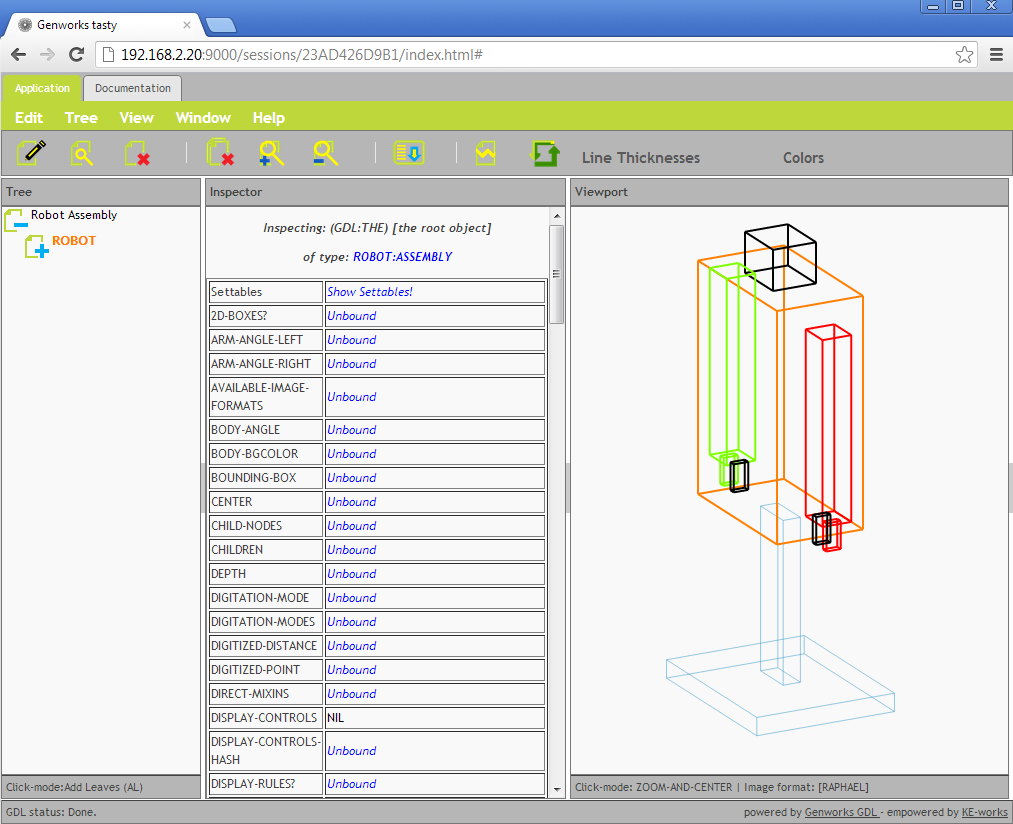
\includegraphics[width=3in,height=3in]{../images/tasty-robot.png}
\end{center}

\caption{Robot displayed in Tasty}

\label{fig:tasty-robot}

\end{figure}

\begin{figure}
\begin{center}
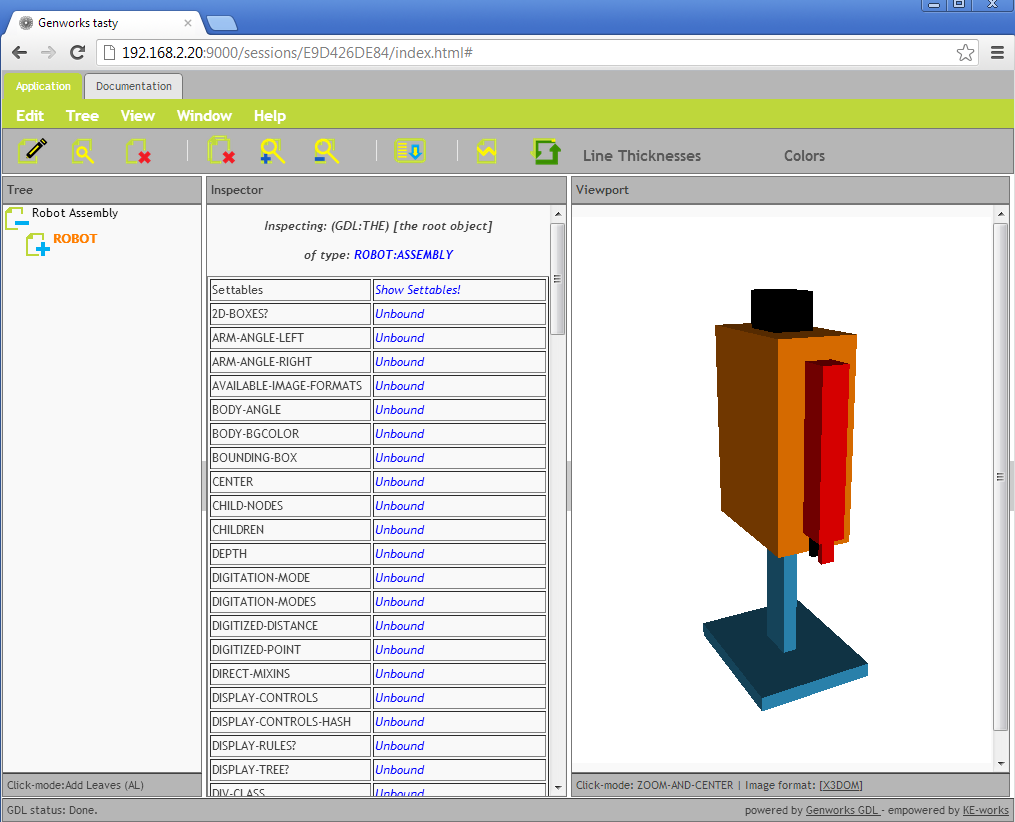
\includegraphics[width=3in,height=3in]{../images/tasty-robot-x3dom.png}
\end{center}

\caption{Robot x3dom}

\label{fig:tasty-robot-x3dom}

\end{figure}

\item Click on the robot to zoom in.

\item Select ``Clear View!'' from the View menu.

\item Select ``X3DOM'' from the View menu.

\item Click on the top node in the tree.

\item ``Refresh'' or ``Reload'' your browser window (may not be necessary).

\item If your browser supports WebGL, you will see the robot in shaded dynamic view as shown in Figure
\ref{fig:tasty-robot-x3dom}.

\item Select ``PNG'' from the View menu. You will see the
	 wireframe view of the robot as a PNG image.

\item Select ``X3D'' from the View menu. If your browser
has an X3D plugin installed (e.g. BS Contact), you will see the robot
in a shaded dynamic view.

\end{enumerate}



\subsection{Full Regression Test}

\label{subsec:fullregressiontest}

\index{regression tests}The following commands will invoke a full regression test,
including a test of the Surface and Solids primitives provided by the
SMLib geometry kernel. Note that the SMLib geometry kernel is only
available with proprietary Genworks GDL licenses --- therefore, if you
have open-source Gendl or a lite Trial version of Genworks GDL, these
regression tests will not all function.

In Emacs at the \texttt{gdl-user} prompt in the \texttt{*slime-repl...*} buffer, type the following commands:

\begin{enumerate}

\item \texttt{(ql:quickload :regression)}

\item \texttt{(gdl-lift-utils::define-regression-tests)}

\item \texttt{(gdl-lift-utils::run-regression-tests-pass-fail)}

\item \texttt{(pprint gdl-lift-utils::*regression-test-report*)}

\end{enumerate}



\section{Getting Help and Support}

\label{sec:gettinghelpandsupport}

If you encounter unexplained errors in the installation and
startup process, please contact the following resources:

\begin{enumerate}

\item Make a posting to the \href{http://groups.google.com/group/genworks}{Genworks Google Group}

\item Join the \#gendl IRC (Internet Relay Chat) channel on
	irc.freenode.net and discuss issues there.

\item For exclusively Common Lisp issues, join the \#lisp
	IRC (Internet Relay Chat) channel on irc.freenode.net and
	discuss issues there.

\item Also for Common Lisp issues, follow the comp.lang.lisp
	Usenet group.

\item If you are a supported Genworks customer, send email to \href{mailto:support@genworks.com}{support@genworks.com}

\item If you are not a supported Genworks customer but you want to report an apparent bug or have other suggestions or inquiries, you may also send email to \href{mailto:support@genworks.com}{support@genworks.com}, but as a non-customer please understand that Genworks
	  cannot guarantee a response or a particular time frame for a
	  response. Also note that we are not able to offer guaranteed
	  support for Trial and Student licenses 

\end{enumerate}



\chapter{Basic Operation of the GDL Environment}

\label{chap:basicoperationofthegdlenvironment}

This chapter will lead you through all the basic steps of
operating a typical GDL-based development environment. We will not in
this section go into particular depth about the additional features of
the environment or language syntax --- this chapter is merely to
familiarize you with, and start you practicing with the nuts and bolts
of operating the environment with a keyboard.

\section{What is Different about GDL?}

\label{sec:whatisdifferentaboutgdl?}

GDL is a \emph{dynamic} language environment with incremental compiling and in-memory
definitions. This means that as long as the system is running you
can \emph{compile} new \emph{definitions} of functions, objects, etc, and they will immediately become
available as part of the running system, and you can begin testing
them immediately, or update an existing set of objects to observe
their new behavior.

In many other programming language systems, to introduce a new
function or object, one has \emph{to start the system from the beginning} and reload all the files in order to test new functionality.
 
In GDL, it is typical to keep the same development session up and
running for an entire day or longer, making it unnecessary to
repeatedly recompile and reload your definitions from scratch. Note,
however, that if you do shut down and restart the system for some
reason, then you will have to recompile and/or reload your
application's definitions in order to bring the system back into a
state where it can instantiate (or ``run'') your application.

While this can be done manually at the command-line, it is typically
done \emph{automatically} in one of two ways:

\begin{enumerate}

\item Using commands placed into
the \texttt{gdlinit.cl} initialization file, as described in Section 
\ref{sec:customizingyourenvironment}.

\item Alternatively, you can compile and load definitions into
your session, then save the ``world'' in that state. That way it is
possible to start a new GDL ``world'' which already has all your
application's definitions loaded and ready for use, without having to
procedurally reload any files. You can then begin to make and test new
definitions (and re-definitions) starting from this new ``world.''
You can think of a saved ``world'' like pre-made cookie dough: no need
to add each ingredient one by one --- just start making cookies!

\end{enumerate}



\section{Startup, ``Hello, World!'' and Shutdown}

\label{sec:startup,hello,world!andshutdown}



The typical GDL environment consists of three programs:

\begin{enumerate}

\item Gnu Emacs (the editor);

\item a Common Lisp engine with GDL system loaded or built into it (e.g. the \texttt{gdl.exe} executable in your \texttt{program/} directory); and

\item (optionally) a web browser such as Firefox, Google
Chrome, Safari, Opera, or Internet Explorer

\end{enumerate}

Emacs runs as the main \emph{process}, and this in turn starts the CL engine with GDL as a \emph{sub-process}. The CL engine typically runs an embedded \emph{webserver}, enabling you to access your application through a standard web browser.



As described in Chapter 
\ref{chap:installation}, the typical way to start a pre-packaged GDL environment is with the \texttt{run-gdl.bat} (Windows), or \texttt{run-gdl} (MacOS, Linux) script files, or with the installed Start
program item (Windows) or application bundle (MacOS). Invoke this
script file from the Start menu (Windows), your computer's file
manager, or from a desktop shortcut if you have created one.  Your
installation executable may also have created a Windows ``Start'' menu
item for Genworks GDL. You can of course also invoke \texttt{run-gdl.bat} from the Windows ``cmd'' command-line, or from another command shell such as Cygwin.\footnote{Cygwin is also useful as a command-line tool on Windows
for interacting with a version control system like Subversion (svn).}


\begin{figure}
\begin{center}
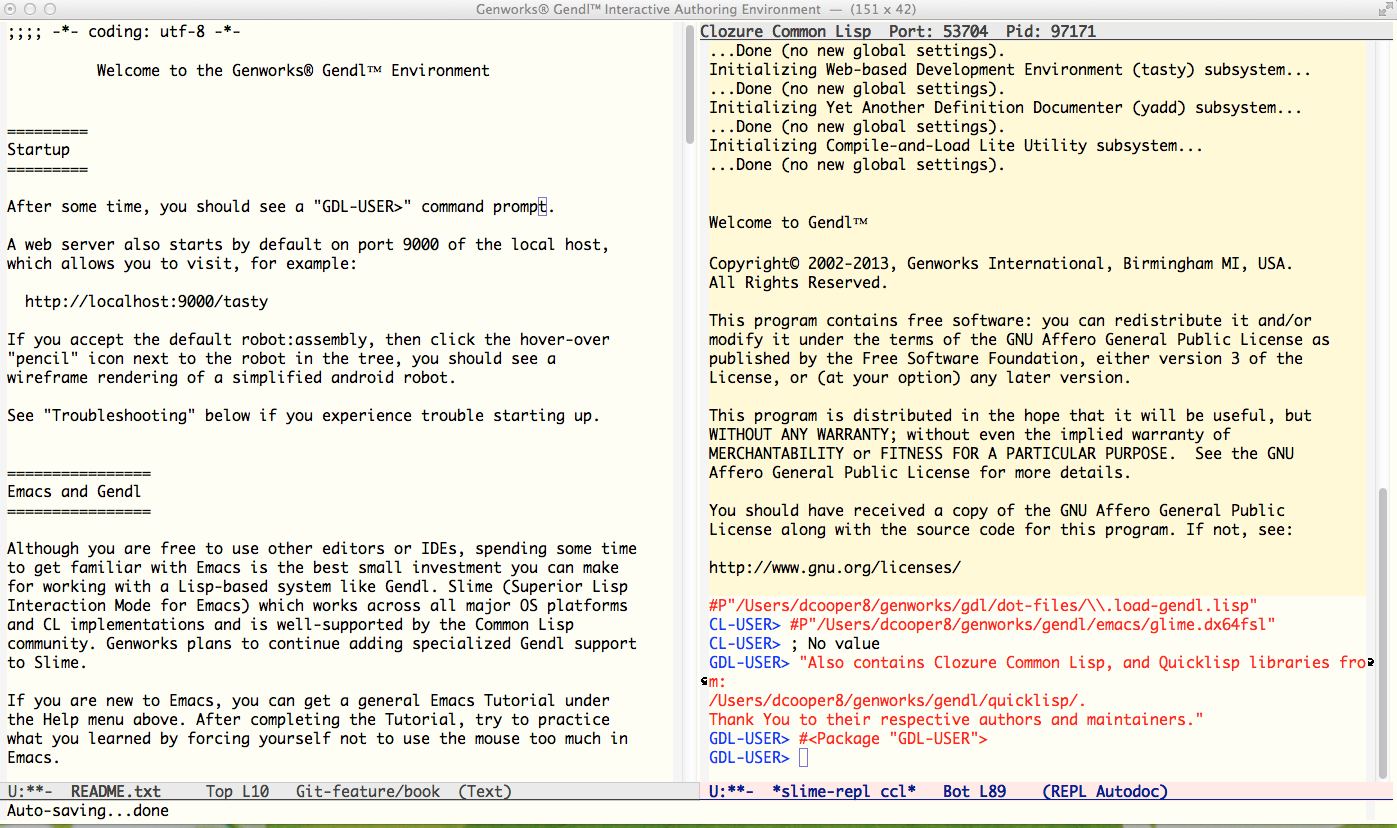
\includegraphics[width=6in,height=4in]{../images/emacs-startup.png}
\end{center}

\caption{Startup of Emacs with GDL}

\label{fig:emacs-startup}

\end{figure}


\subsection{Startup}

\label{subsec:startup}

 Startup of a typical GDL development session consists of
two fundamental steps: (1) starting the Emacs editing environment,
and (2) starting the actual GDL process as a ``sub-process'' or ``inferior'' process 
within Emacs. The GDL process should automatically establish a network connection
back to Emacs, allowing you to interact directly with the GDL process from within Emacs.

\begin{enumerate}

\item Invoke the \texttt{run-gdl.bat}, \texttt{run-gdl.bat}
startup script, or the provided executable from the Start
menu (windows) or application bundle (Mac).

\item You should see an emacs window similar to that shown in Figure 
\ref{fig:emacs-startup}. (alternative colors are also possible).

\item (MS Windows): Look for the Genworks GDL Console
window, or (Linux, Mac) use the Emacs ``Buffer'' menu to visit the
``*inferior-lisp*'' buffer. Note that the Genworks GDL Console
window might start as a minimized icon; click or double-click it to
un-minimize.

\item Watch the Genworks GDL Console window for any
errors. Depending on your specific installation, it may take from a
few seconds to several minutes for the Genworks GDL Console (or
*inferior-lisp* buffer) to settle down and give you a \texttt{gdl-user(): } prompt. This window is where you will see most of your program's textual output, any 
error messages, warnings, etc.

\item In Emacs, type: \texttt{C-x \&} (or select Emacs menu item \emph{Buffers$\rightarrow$*slime-repl...*}) to visit the ``*slime-repl ...*'' buffer. The full name
of this buffer depends on the specific CL/GDL platform which you are
running. This buffer contains an interactive prompt, labeled \texttt{gdl-user>}, where you will enter most of your commands to interact with your running GDL session
for testing, debugging, etc. There is also a web-based graphical interactive environment called \emph{tasty} which will be discussed in Chapter 
\ref{chap:thetastydevelopmentenvironment}.

\item To ensure that the GDL command prompt is up and running, type: \texttt{(+ 2 3)} and press [Enter].

\item You should see the result \texttt{5} echoed back to you below the prompt.

\end{enumerate}



\subsection{Developing and Testing a  ``Hello World'' application}

\label{subsec:developingandtestingahelloworldapplication}

 

\begin{enumerate}

\item type C-x (Control-x) 2, or C-x 3, or use the ``Split
Screen'' option of the File menu to split the Emacs frame into two
``windows'' (``windows'' in Emacs are non-overlapping panels, or
rectangular areas within the main Emacs window).

\item type C-x o several times to move from one window to
the other, or move the mouse cursor and click in each window. Notice
how the blinking insertion point moves from one window to the other.

\item In the top (or left) window, type C-x C-f (or select Emacs menu item
``File$\rightarrow$Open File'') to get the ``Find file'' prompt in the
mini-buffer.

\item Type C-a to move the point to the beginning of the mini-buffer line.

\item Type C-k to delete from the point to the end of the mini-buffer.

\item Type \texttt{\textasciitilde/hello.gdl} and press [Enter]

\item You are now editing a (presumably new) file of GDL
	 code, located in your HOME directory, called \texttt{hello.gdl}

\item Enter the text from Figure 
\ref{fig:simpleobjectdefinition} into the \texttt{hello.gdl} buffer. You do not have to match the line breaks and whitespace as shown in the example.
You can auto-indent each new line by pressing [TAB] after pressing [Enter] for the newline.

\emph{Protip:}You can also try using \texttt{C-j} instead of [Enter], which will automatically give a newline and auto-indent.



\begin{figure}
\begin{lrbox}{\boxedverb}
\begin{minipage}{\linewidth}

\begin{verbatim}
 (in-package :gdl-user)

 (define-object hello ()

   :computed-slots 
   ((greeting "Hello, World!")))

\end{verbatim}
\end{minipage}
\end{lrbox}
\fbox{\usebox{\boxedverb}}

\caption{Example of Simple Object Definition}

\label{fig:simpleobjectdefinition}

\end{figure}

\item type \texttt{C-x C-s} (or choose Emacs menu item \emph{File$\rightarrow$Save}) to save the contents of the buffer (i.e. the window) 
to the file in your HOME directory.

\item type \texttt{C-c C-k} (or choose Emacs menu item \emph{SLIME$\rightarrow$Compilation$\rightarrow$Compile/Load File}) to compile \& load the code from this file.

\item type \texttt{C-c o} (or move and click the mouse)  to switch to the bottom window.

\item In the bottom window, type \texttt{C-x \&} (or choose Emacs menu item \emph{Buffers$\rightarrow$*slime-repl...*}) to get the \texttt{*slime-repl ...*} buffer, which should contain a \texttt{gdl-user>} prompt. This is where you normally type interactive GDL commands.

\item If necessary, type \texttt{M \textgreater} (that is, hold down Meta (Alt), Shift, and the ``\textgreater'' key) to
move the insertion point to the end of this buffer.

\item At the \texttt{gdl-user>} prompt, type 

\begin{verbatim}(make-self 'hello)
\end{verbatim} and press [Enter].

\item At the \texttt{gdl-user>} prompt, type 

\begin{verbatim}(the greeting)
\end{verbatim} and press [Enter].

\item You should see the words \texttt{Hello, World!} echoed back to you below the prompt.

\end{enumerate}



\subsection{Shutdown}

\label{subsec:shutdown}

 To shut down a development session gracefully, you should first shut down the GDL process,
then shut down your Emacs.

\begin{itemize}

\item Type \texttt{M-x quit-gdl} (that is, hold Alt and press X, then release both while you type \texttt{quit-gdl} in the mini-buffer), then press [Enter]

\item alternatively, you can type \texttt{C-x \&} (that is, hold Control and press X, then release both while you type \&. 
This will visit the *slime-repl* buffer. Now type: \texttt{, q} to quit the GDL session.

\item Finally, type \texttt{C-x C-c} to quit from Emacs. Emacs will prompt you to save any
	   modified buffers before exiting.

\end{itemize}



\section{Working with Projects}

\label{sec:workingwithprojects}

GDL contains utilities which allow you to treat your
application as a ``project,'' with the ability to compile,
incrementally compile, and load a ``project'' from a directory tree of
source files representing your project. In this section we provide an
overview of the expected directory structure and available control
files, followed by a reference for each of the functions included in
the bootstrap module.

\subsection{Directory Structure}

\label{subsec:directorystructure}



You should structure your applications in a modular
fashion, with the directories containing actual Lisp sources called
"source." You may have subdirectories which themselves contain
"source" directories. We recommend keeping your codebase directories
relatively flat, however.



In Figure 
\ref{fig:yoyodyne-base} is an example application directory, with four source files.


\begin{figure}
\begin{lrbox}{\boxedverb}
\begin{minipage}{\linewidth}

\begin{verbatim}
  apps/yoyodyne/booster-rocket/source/assembly.gdl
  apps/yoyodyne/booster-rocket/source/package.gdl
  apps/yoyodyne/booster-rocket/source/parameters.gdl
  apps/yoyodyne/booster-rocket/source/rules.gdl

\end{verbatim}
\end{minipage}
\end{lrbox}
\fbox{\usebox{\boxedverb}}

\caption{Example project directory with four source files}

\label{fig:yoyodyne-base}

\end{figure}


\subsection{Source Files within a source/ subdirectory}

\label{subsec:sourcefileswithinasource/subdirectory}



\subsubsection{Enforcing Ordering}

\label{subsubsec:enforcingordering}



Within a source subdirectory, you may have a file called \texttt{file-ordering.isc}\footnote{\texttt{isc} stands for ``Intelligent Source Configuration''} to enforce a certain ordering of the files. Here are
the contents of an example for the above application:



\begin{verbatim}("package" "parameters")
\end{verbatim}

This will force package.lisp to be compiled/loaded first, and
parameters.lisp to be compiled/loaded next. The ordering on the rest
of the files should not matter (although it will default to
lexigraphical ordering).



Now our sample application directory appears as in
	Figure 
\ref{fig:yoyodyne-with-file-ordering-isc}.


\begin{figure}
\begin{lrbox}{\boxedverb}
\begin{minipage}{\linewidth}

\begin{verbatim}
  apps/yoyodyne/booster-rocket/source/assembly.gdl
  apps/yoyodyne/booster-rocket/source/file-ordering.isc
  apps/yoyodyne/booster-rocket/source/package.gdl
  apps/yoyodyne/booster-rocket/source/parameters.gdl
  apps/yoyodyne/booster-rocket/source/rules.gdl
\end{verbatim}
\end{minipage}
\end{lrbox}
\fbox{\usebox{\boxedverb}}

\caption{Example project directory with file ordering configuration file}

\label{fig:yoyodyne-with-file-ordering-isc}

\end{figure}


\subsection{Generating an ASDF System}

\label{subsec:generatinganasdfsystem}



ASDF stands for Another System Definition Facility, which
	is the predominant system in use for Common Lisp third-party
	libraries. With GDL, you can use the \texttt{:create-asd-file?} keyword argument to make cl-lite generate an ASDF system
file instead of actually compiling and loading the system. For example: 

\begin{verbatim}(cl-lite "apps/yoyodyne/" :create-asd-file? t)
\end{verbatim}



In order to include a depends-on clause in your ASDF system file, create a file called \texttt{depends-on.isc} in the toplevel directory of your system. In this file,
place a list of the systems your system depends on. This can be
systems from your own local projects, or from third-party libraries.
For example, if your system depends on the \texttt{:cl-json} third-party library, you would have the following contents in your \texttt{depends-on.isc}: 

\begin{verbatim}(:cl-json)
\end{verbatim}



\subsection{Compiling and Loading a System}

\label{subsec:compilingandloadingasystem}

Once you have generated an ASDF file, you can compile and
load the system using Quicklisp. To do this for our example, follow these steps:

\begin{enumerate}

\item 

\begin{verbatim}(cl-lite "apps/yoyodyne/" :create-asd-file? t)
\end{verbatim} to generate the asdf file for the yoyodyne system. This only has to be done once after every time you add, remove, or rename a file or folder from the system.

\item 

\begin{verbatim}(pushnew "apps/yoyodyne/" ql:*local-project-directories* :test #'equalp)
\end{verbatim} This can be done in your \texttt{gdlinit.cl} for projects you want available during every development session. Note that you should include
the full path prefix for the directory containing the ASDF system file.

\item 

\begin{verbatim}(ql:quickload :gdl-yoyodyne)
\end{verbatim} This will compile and load the actual system. Quicklisp
uses ASDF at the low level to compile and load the systems, and
Quicklisp will retrieve any depended-upon third-party libraries from
the Internet on-demand.  Source files will be compiled only if the
corresponding binary (fasl) file does not exist or is older than the
source file. By default, ASDF keeps its binary files in a  \emph{cache} directory, separated according to the CL platform and
operating system. The location of this cache is system-dependent, but
you can see where it is by observing the compile and load
process.

\end{enumerate}



\section{Customizing your Environment}

\label{sec:customizingyourenvironment}

 You may customize your environment in several different ways,
for example by loading definitions and settings into your GDL
``world'' automatically when the system starts, and by specifying
fonts, colors, and default buffers (to name a few) for your emacs
editing environment.

\section{Saving the World}

\label{sec:savingtheworld}

``Saving the world'' refers to a technique of saving a complete
binary image of your GDL ``world'' which contains all the currently
compiled and loaded definitions and settings.  This allows you to
start up a saved world almost instantly, without being required to
reload all the definitions. You can then incrementally compile and
load just the particular definitions which you are working on for your
development session.

To save a world, follow these steps:

\begin{enumerate}

\item Load the base GDL code and (optionally) code for GDL
modules (e.g. gdl-yadd, gdl-tasty) you want to be in your saved
image. Note that in some implementations, this has step to be done in
a plain session without multiprocessing (i.e. without an Emacs
connection) - so you would do this loading step from a command shell
e.g. Windows cmd prompt. For example:

\begin{verbatim}
 (ql:quickload :gdl-yadd) 
 (ql:quickload :gdl-tasty)
\end{verbatim}

\item (needed only for full GDL):

\begin{verbatim}(ff:unload-foreign-library (merge-pathnames "smlib.dll" "sys:smlib;"))
\end{verbatim}

\item 

\begin{verbatim}(net.aserve:shutdown)
\end{verbatim}

\item  (to save an image named yoyodyne.dxl) Invoke the command 

\begin{verbatim}(ensure-directories-exist "~/gdl-images/")
\end{verbatim}

\begin{verbatim}(uiop:dump-image dumplisp "~/gdl-images/yoyodyne")
\end{verbatim}Note that the standard extension for Allegro CL images is \texttt{.dxl}. Prepend the file name with path information, to write the image to a specific location.

\end{enumerate}



\section{Starting up a Saved World}

\label{sec:startingupasavedworld}

In order to start up GDL using a custom saved image, or ``world,'' follow these steps

\begin{enumerate}

\item Exit GDL

\item Copy the supplied image file, e.g.\texttt{gdl.dxl} to \texttt{gdl-orig.dxl}.

\item Move the custom saved dxl image to \texttt{gdl.dxl} in the GDL application \texttt{"program/"} directory.

\item Start GDL as usual. Note: you may have to edit the system gdlinit.cl or your home gdlinit.cl
to stop it from loading redundant code which is already in the saved image.

\end{enumerate}



\chapter{Understanding Common Lisp}

\label{chap:understandingcommonlisp}



GDL is a superset of Common Lisp (CL) --- that is, all of
CL is available to you during development, and is available to your
applications at runtime (i.e. after they are deployed). The
lowest-level expressions in a GDL definition are CL ``symbolic
expressions,'' or ``S-expressions.''  This chapter will familiarize
you with CL S-expressions.



\section{S-expression Fundamentals}

\label{sec:s-expressionfundamentals}



S-expressions can be used in a similar manner to Formulas
in a Spreadsheet to establish the value of a particular \emph{slot} (i.e. named data value) in an object. However, unlike in
a spreadsheet, these values are only computed on an as-needed
basis (i.e. ``on-demand''). You can also evaluate S-expressions at the
toplevel \texttt{gdl-user\textgreater} prompt, and see the result immediately. In fact, this toplevel prompt is called a \emph{read-eval-print} loop, because its purpose is to \emph{read} each S-expression  entered, \emph{evaluate} the expression to yield a result (or \emph{return-value}), and finally to \emph{print} that result.



CL S-expressions use a  \emph{prefix} notation, which means that they consist of either an \emph{atom} (e.g.  number, text string, symbol) or a \emph{list} (one or more items enclosed by parentheses, where the
	  first item is taken as a symbol which names an
	  operator). Here is an example: 

\begin{verbatim}(+ 2 2)
\end{verbatim}This expression consists of the function named by the symbol \texttt{+}, followed by the numeric arguments \texttt{2} and another \texttt{2}. As you may have suspected, when this expression is
evaluated it will return the value 4.\emph{Try it: }try typing this expression at your command prompt, and see
the return-value being printed on the console. What is actually
occurring here? When CL is asked to evaluate an expression, it
processes the expression according to the following rules:





\begin{itemize}

\item If the expression is an \emph{atom} (e.g. a non-list datatype such as a number, text
string, or literal symbol), it simply returns itself as its evaluated
value. Examples: 

\begin{itemize}

\item 

\begin{verbatim}gdl-user> 99
99
\end{verbatim}

\item 

\begin{verbatim}gdl-user> 99.9
99.9
\end{verbatim}

\item 

\begin{verbatim}gdl-user> 3/5
3/5
\end{verbatim}

\item 

\begin{verbatim}gdl-user> "Bob"
"Bob"
\end{verbatim}

\item 

\begin{verbatim}gdl-user> "Our golden rule is simplicity"
"Our golden rule is simplicity"
\end{verbatim}

\item 

\begin{verbatim}gdl-user> 'my-symbol
my-symbol
\end{verbatim}

\end{itemize}

Note that numbers are represented directly (with decimal
points and slashes for fractions allowed), strings are surrounded by
double-quotes, and literal symbols are introduced with a preceding
single-quote. Symbols are allowed to have dashes (``-'') and most
other special characters. By convention, the dash is used as a word
separator in CL symbols.

\item If the expression is a \emph{list} (i.e. is surrounded by parentheses), CL processes
the \emph{first} element in this list as an \emph{operator name}, and the \emph{rest} of the elements in the list represent the \emph{arguments} to the operator. An operator can take zero or more
arguments, and can return zero or more return-values. Some operators
evaluate their arguments immediately and work directly on those
values (these are called \emph{functions}). Other operators expand into other code. These are called \emph{special operators} or \emph{macros}. Macros are what give Lisp (and CL in particular) its
special power. Here are some examples of functional S-expressions: 

\begin{itemize}

\item 

\begin{verbatim}gdl-user> (expt 2 5)
32
\end{verbatim}

\item 

\begin{verbatim}gdl-user> (+ 2 5)
7
\end{verbatim}

\item 

\begin{verbatim}gdl-user> (+ 2)
2
\end{verbatim}

\item 

\begin{verbatim}gdl-user> (+ (+ 2 2) (+ 3 3 ))
10
\end{verbatim}

\end{itemize}



\end{itemize}





\section{Fundamental CL Data Types}

\label{sec:fundamentalcldatatypes}



As has been noted, Common Lisp natively supports many data
types\footnote{See http://en.wikipedia.org/wiki/Data\_type for
a more detailed discussion of what is meant by ``data types'' in this
context.} common to other languages, such as numbers and text strings. CL
also contains several \emph{compound} data types such as lists, arrays, and hash tables. CL
contains \emph{symbols} as well, which typically are used as names for other data elements.



Regarding data types, CL follows a system called dynamic
typing. Basically this means that values have type, but variables do
not necessarily have type, and typically variables are not
``pre-declared'' to be of a particular type. For example, a
variable (or slot name in GDL) called \texttt{length} could contain a value \texttt{42} (an integer), \texttt{42.43} (a floating-point number), \texttt{3/16} (a rational number), or even \texttt{:long} (a descriptive keyword symbol).



\subsection{Numbers}

\label{subsec:numbers}



As observed, numbers in CL are a native data type which
simply evaluate to themselves when entered at the toplevel or included
in an expression.



Numbers in CL form a hierarchy of types, which includes Integers,
Ratios, Floating Point, and Complex numbers. For many purposes, you
only need to think of a value as a ``number'' without getting any more
specific than that. Most arithmetic operations, such as \texttt{+}, \texttt{-}, \texttt{*}, \texttt{/} etc, will automaticaly do any necessary type-coercion on their
arguments and will return a number of the appropriate type.

CL supports a full range of floating-point decimal numbers, as well as
true Ratios, which means that, for example, \texttt{1/3} is a true one-third, not \texttt{0.333333333} rounded off at some arbitrary precision short of
	    infinity.



\subsection{Strings}

\label{subsec:strings}



Strings are actually a specialized kind of
array, namely a one-dimensional array (vector) made up of text
characters. These characters can be letters, numbers, or punctuation,
and in some cases can include characters from international character
sets (e.g. Unicode or UTF-8) such as Chinese Hanzi or Japanese
Kanji. The string delimiter in CL is the double-quote character.



Text strings in CL are a native data type which simply
evaluate to themselves when included in an expression.



A common way to produce a string in CL is with the \texttt{format} function. Although the \texttt{format} function can be used to send output to any kind of destination, or \emph{stream}, it will simply yield a string if you specify \texttt{nil} for the stream. Example: 
{\small

\begin{verbatim}
 gdl-user> (format nil "The time is: ~a" (get-universal-time))
 "The time is: 3564156603"
 gdl-user> (format nil "The time is: ~a" (iso-8601-date (get-universal-time)))
 "The time is: 2012-12-10"
 gdl-user> (format nil "The time is: ~a" (iso-8601-date (get-universal-time) :include-time? t))
 "The time is: 2012-12-10T14:30:17"
\end{verbatim}}



As the above example demonstrates, \texttt{format} takes a \emph{stream designator} or \texttt{nil} as its first argument, then a \emph{format-string}, then enough arguments to match the \emph{format directives} in the format-string. Format directives begin with the
tilde character (\texttt{~}).  The format-directive \texttt{~a} indicates that the printed representation of the corresonding argument should simpy be 
substituted into the format-string at the point where it occurs.



We will cover more details on \texttt{format} in Section 
\ref{sec:input-output} on Input/Output, but for now, a familiarity with the simple use of \texttt{(format nil ...)} will be helpful for Chapter 
\ref{chap:understandinggdl---coregdlsyntax}.



\subsection{Symbols}

\label{subsec:symbols}



Symbols are such an important data structure in CL that people
sometimes refer to CL as a ``Symbolic Computing Language.'' Symbols
are a type of CL object which provides your program with a built-in
capacity to store and retrieve values and functions, as well as being
useful in their own right. A symbol is most often known by its name
 (actually a string), but in fact there is much more to a symbol than
its name. In addition to the name, symbols also contain a \emph{function} slot, a \emph{value} slot, and an open-ended \emph{property-list} slot in which you can store an arbitrary number of named properties.



For a named function such as \texttt{+} the function-slot contains the actual function
object for performing numeric addition. The value-slot of a symbol can
contain any value, allowing the symbol to act as a global variable, or \emph{parameter}. And the property-list, also known as the \emph{plist} slot, can contain an arbitrary amount of information.



This separation of the symbol data structure into \emph{function}, \emph{value}, and \emph{plist} slots is one fundamental distinction between Common Lisp
and most other Lisp dialects. Most other dialects allow only one (1)
``thing'' to be stored in the symbol data structure, other than its
name (e.g. either a function or a value, but not both at the same
time). Because Common Lisp does not impose this restriction it is not
necessary to contrive names, for example for your variables, to avoid
conflicting with existing ``reserved words'' in the system. For
example, \texttt{list} is the name of a built-in function in CL, but you may
freely use \texttt{list} as a variable name as well. There is no need to
contrive arbitrary abbreviations such as \texttt{lst}.



How symbols are evaluated depends on where they are
located in an expression. As we have seen, if a \emph{symbol} appears first in a list expression, as with the \texttt{+} in \texttt{(+ 2 2)}, the symbol is evaluated for its function slot. If the
first element of an expression indeed has an identified \emph{function} in its function slot, then any 
subsequent symbol in the expression is taken as a variable, and it is evaluated 
for its global or local value, depending on its scope (more on variables and 
scope later).



As noted in Section 3.1.3, if you want a literal symbol itself, one
way to achieve this is to ``quote'' the symbol name:

\begin{verbatim}'a
\end{verbatim}



Another way is for the symbol to appear within a quoted list expression, for example:

\begin{verbatim}'(a b c)
\end{verbatim} or 

\begin{verbatim}'(a (b c) d)
\end{verbatim}



Note that the quote (\texttt{'}) applies across everything in the list expression, including any sub- expressions.



\subsection{List Basics}

\label{subsec:listbasics}



Lisp derives its name from its strong support for the
list data structure. The list concept is important to Common Lisp (CL)
for more than this reason alone --- most notably, lists are important
because \emph{all CL programs are themselves lists.}



 Having the list as a native data structure, as well as the form of all
programs, means that it is straightforward for CL programs to compute
and generate other CL programs. Likewise, CL programs can read and
manipulate other CL programs in a natural manner. This cannot be said
of most other languages, and is one of the primary distinguishing
characteristics of Lisp as a language.



Textually, a \emph{list} is defined as zero or more items surrounded by
parentheses. The items can be objects of any valid CL data types, such
as numbers, strings, symbols, lists, or other kinds of
objects. According to standard evaluation rules, you must quote a
literal list to evaluate it as such, or CL will assume you are calling
a \emph{function}. Now look at the following list:

\begin{verbatim}(defun hello () (write-string "Hello, World!"))
\end{verbatim}This list also happens to be a valid CL program (function definition,
in this case). Don't concern yourself about analyzing the function definition
right now, but do take a few moments to convince yourself that it
meets the requirements for a list.



What are the types of the elements in this list?\footnote{Answer: symbol, symbol, (empty) list, list with symbol and string.}



In addition to using the quote (') to produce a literal list, another
way to produce a list is to call the function \texttt{list}. The function \texttt{list} takes any number of arguments, and returns a list made up
from the result of evaluating each argument. As with all functions,
the arguments to the \texttt{list} function get evaluated, from left to right, before being
processed by the function. For example:

\begin{verbatim}(list 'a 'b (+ 2 2))
\end{verbatim}will return the list

\begin{verbatim}(a b 4)
\end{verbatim}The two quoted symbols evaluate to symbols, and the function
call \texttt{(+ 2 2)} evaluates to the number 4.



\subsection{The List as a Data Structure}

\label{subsec:thelistasadatastructure}

In this section we will discuss a few of the fundamental native
CL operators for manipulating lists as data structures. These include
operators for doing things such as:

\begin{enumerate}

\item finding the length of a list;

\item accessing particular members of a list;

\item appending multiple lists together to make a new list.

\end{enumerate}



\subsubsection{Finding the Length of a List}

\label{subsubsec:findingthelengthofalist}

The function \texttt{length} will return the length of any type of sequence, including a list:

\begin{verbatim}gdl-user> (length '(a b c d e f g h i j)
10
gdl-user> (length nil)
0
\end{verbatim}Note that \texttt{nil} qualifies as a list (albeit the empty list), so taking its length yields the integer \texttt{0}.

\subsubsection{Accessing the Elements of a List}

\label{subsubsec:accessingtheelementsofalist}

Common Lisp defines the accessor functions \texttt{first} through \texttt{tenth} as a means of accessing the first ten elements in a list:

\begin{verbatim}
gdl-user> (first '(a b c))

a

gdl-user> (second '(a b c))

b

gdl-user> (third '(a b c))

c
\end{verbatim}For accessing elements in an arbitrary position in the list, you can use the function nth,
which takes an integer and a list as its two arguments:

\begin{verbatim}

gdl-user> (nth 0 '(a b c))

a

gdl-user> (nth 1 '(a b c))

b

gdl-user> (nth 2 '(a b c))

c
\end{verbatim}Note that nth starts its indexing at zero (0), so \texttt{(nth 0 ...)} is equivalent to \texttt{(first ...)}and \texttt{(nth 1 ...)} is equivalent to \texttt{(second ...)}, etc.

\subsubsection{Using a List to Store and Retrieve Named Values}

\label{subsubsec:usingalisttostoreandretrievenamedvalues}

Lists can also be used to store and retrieve named values. When a list is used in this way, 
it is called a \emph{plist}. Plists contain pairs of elements, where each pair consists of a \emph{key} and some \emph{value}. The key is typically an actual keyword symbol --- that is,
a symbol preceded by a colon (:). The value can be any value, such as
a number, a string, or even a GDL object representing something
complex such as an aircraft.

A plist can be constructed in the same manner as any list, e.g. with the \texttt{list} operator:

\begin{verbatim}(list :a 10 :b 20 :c 30)
\end{verbatim}In order to access any element in this list, you can use the \texttt{getf} operator. The \texttt{getf} operator is specially intended for use with plists:

\begin{verbatim}gdl-user> (getf (list :a 10 :b 20 :c 30) :b
20
gdl-user> (getf (list :a 10 :b 20 :c 30) :c
30
\end{verbatim} Common Lisp contains several other data structures for mapping keywords or numbers to values, such
as \emph{arrays} and \emph{hash tables}. But for relatively short lists, and especially for rapid prototyping and testing work, plists
can be useful. Plists can also be written and read (i.e. saved and restored) to and from plain text files
in your filesystem, in a very natural way.

\subsubsection{Appending Lists}

\label{subsubsec:appendinglists}

The function \texttt{append} takes any number of lists, and returns a new list which results from
appending them together. Like many CL functions, append does not \emph{side-effect}. That is, it simply returns a new list as a return-value, but does not modify its 
arguments in any way:

\begin{verbatim}
 gdl-user> (defparameter my-slides '(introduction welcome lists functions))
 (introduction welcome lists functions)

 gdl-user> (append my-slides '(numbers))
 (introduction welcome lists functions numbers)

 gdl-user> my-slides
 (introduction welcome lists functions)
\end{verbatim}Note that the simple call to \texttt{append} does not affect the variable \texttt{my-slides}. Later we will observe how one may alter the value of a
variable such as \texttt{my-slides}.

\section{Summary}

\label{sec:summary}

In this chapter we have presented enough basics of Lisp's
minimal syntax, and some particulars of Common Lisp, to enable you to
start with the Genworks GDL framework. In keeping with the
demand-driven philosophy of GDL, subsequent chapters will cover additional
CL material on an as-needed basis.

\chapter{Understanding GDL --- Core GDL Syntax}

\label{chap:understandinggdl---coregdlsyntax}



Now that you have a basic familiarity with Common Lisp
      syntax (or, more accurately, the \emph{absence} of syntax), we will move directly into the Genworks GDL
framework. By using GDL you can formulate most of your engineering and
computing problems in a natural way, without becoming involved in the
complexity of the Common Lisp Object System (CLOS).



As discussed in the previous chapter, GDL is based on and
is a superset of ANSI Common Lisp. Because ANSI CL is unencumbered and
is an open standard, with several commercial and free implementations,
it is a good wager that applications written in it will continue to be
usable for the balance of this century, and beyond. Many commercial
products have a shelf life only until a new product comes along. Being
based in ANSI Common Lisp ensures GDL's permanence.



[The GDL product is a commercially available KBE system
with Proprietary licensing.  The Gendl Project is an open-source
Common Lisp library which contains the core language kernel of GDL,
and is licensed under the terms of the Affero Gnu Public License. The
core GDL language is a proposed standard for a vendor-neutral KBE
language.]



\section{Defining a Working Package}

\label{sec:definingaworkingpackage}



In Common Lisp, \emph{packages} are a mechanism to separate symbols into
namespaces. Using packages it is possible to avoid ``naming'' conflicts in
large projects. Consider this analogy: in the United States, telephone
numbers are preceded by a three-digit area code and then consist of a
seven-digit number. The same seven-digit number can occur in two or
more separate area codes, without causing a conflict.



The macro \texttt{gdl:define-package} is used to set up a new working package in GDL.



 



Example:

\begin{verbatim}(gdl:define-package :yoyodyne)
\end{verbatim} will establish a new package (i.e. ``area code'')
called \texttt{:yoyodyne} which has all the GDL operators available.



The \texttt{:gdl-user} package is an empty, pre-defined package for your use if
you do not wish to make a new package just for scratch work.



For real projects it is recommended that you make and work in your own
GDL package, defined as above with \texttt{gdl:define-package}.



\emph{A Note for advanced users:} Packages defined with \texttt{gdl:define-package} will implicitly \emph{use} the \texttt{:gdl} package and the \texttt{:common-lisp} package, so you will have access to all exported symbols
  in these packages without prefixing them with their package name.

  You may extend this behavior, by calling \texttt{gdl:define-package} and adding additional packages to use with \texttt{(:use ...)}.  For example, if  you want to work in a package with access to GDL operators,
 Common Lisp operators, and symbols from the \texttt{:cl-json} package \footnote{CL-JSON is a free third-party library for handling JSON format, a common data format used 
for Internet applications.}, you could set it up as follows:

\begin{verbatim} (ql:quickload :cl-json)
 (gdl:define-package :yoyodyne (:use :cl-json))
\end{verbatim}The first form ensures that the cl-json code module is
actually fetched and loaded. The second form defines a package with
the \texttt{:cl-json} operators available to it.



\section{Define-Object}

\label{sec:define-object}

\index{objects!defining}\emph{\index{Define-object}Define-object} is the basic macro for defining objects in GDL. An object 
definition maps directly into a Lisp (CLOS) class definition. 

The \texttt{define-object} macro takes three basic arguments:

\begin{itemize}

\item a \emph{name}, which is a symbol;

\item a \emph{\index{mixin-list}mixin-list}, which is a list of symbols naming other objects from which the current object 
will inherit characteristics;

\item a \emph{\index{specification-plist}specification-plist}, which is spliced in (i.e.\ doesn't have its own surrounding 
parentheses) after the mixin-list, and describes
the object model by specifying properties of the object (messages, contained objects, etc.)
The specification-plist typically makes up the bulk of the object definition.

\end{itemize}



Here are descriptions of the most common keywords making up the specification-plist:

\begin{description}

\item [\index{input-slots}input-slots]
specify information to be passed into the object instance when it is created.

\item [\index{computed-slots}computed-slots]
are actually cached methods, with expressions to compute and return a value.

\item [\index{objects}objects]
specify other instances to be ``contained'' within this instance.

\item [\index{functions}functions]
are (uncached) functions ``of'' the object, i.e.\ they
operate just as normal CL functions, and accept arguments just like
normal CL functions, with the added feature that you can also use \emph{the} referencing, to refer to messages or reference chains
	  which are available to the current object.

\end{description}

Figure 
\ref{fig:object-hello} shows a simple example, which contains two input-slots, \texttt{first-name} and \texttt{last-name}, and a single computed-slot, \texttt{greeting}.
\begin{figure}
\begin{lrbox}{\boxedverb}
\begin{minipage}{\linewidth}

\begin{verbatim}


 (define-object hello ()
   :input-slots (first-name last-name)

   :computed-slots 
   ((greeting (format nil "Hello, ~a ~a!!" 
                     (the first-name) 
                     (the last-name)))))

\end{verbatim}
\end{minipage}
\end{lrbox}
\fbox{\usebox{\boxedverb}}

\caption{Example of Simple Object Definition}

\label{fig:object-hello}

\end{figure}
A GDL Object is analogous in some ways to a CL \texttt{defun}, where the input-slots are like arguments to the function,
and the computed-slots are like return-values. But seen another way,
each slot in a GDL object serves as function in its own right.

The referencing macro \texttt{\index{the}the} shadows CL's \texttt{the} (which is a seldom-used type declaration operator). \texttt{The} in GDL is a macro which is used to reference the value of other messages 
within the same object or within contained objects. In the above example, we are using \texttt{the} to refer to the values of the messages (input-slots) named \texttt{first-name} and \texttt{last-name}. 

Note that messages used with \texttt{the} are given as symbols. These symbols are unaffected by the current Lisp \texttt{*package*}, so they can be specified either as plain unquoted symbols or as keyword
symbols (i.e.\ preceded by a colon), and the \texttt{the} macro will process them appropriately.

\section{Making Instances and Sending Messages}

\label{sec:makinginstancesandsendingmessages}

Once we have defined an object, such as the example above, we can use
the constructor function \texttt{\index{make-object}make-object} in order to create an \emph{instance} of it. \emph{Instance}, in this context, means a single occurence of the object with
tangible values assigned to its input-slots. By way of analogy: an \emph{object definition} is like a blueprint for a house; an \emph{instance} is like an actual house. The \texttt{make-object} function is very similar to the CLOS \texttt{\index{make-instance}make-instance} function. Here we create an instance of \texttt{hello} with specified values for \texttt{first-name} and \texttt{last-name} (the required input-slots), and assign this instance as the value of the symbol \texttt{my-instance}:

\begin{verbatim}
 GDL-USER(16): (setq my-instance
                 (make-object 'hello :first-name "John" 
                                     :last-name "Doe"))
 #<HELLO @ #x218f39c2>
\end{verbatim}Note that keyword symbols are used to ``tag'' the input values. And the return-value of \emph{make-object} is an instance of class \texttt{hello}. Now that we have an instance, we can use the operator \texttt{\index{the-object}the-object} to send messages to this instance:

\begin{verbatim}
 GDL-USER(17): (the-object my-instance greeting)
 "Hello, John Doe!!"
\end{verbatim}\texttt{The-object} is similar to \texttt{the}, but as its first argument it takes an expression which evaluates to an
object instance. \texttt{The}, by contrast, assumes that the object instance is the lexical variable \texttt{\index{self}self}, which is automatically set within the lexical context of a \texttt{define-object}.

Like \texttt{the}, \texttt{the-object} evaluates all but the first of its arguments as package-immune symbols,
so although keyword symbols may be used, this is not a requirement, and plain,
unquoted symbols will work just fine.

For convenience, you can also set \texttt{self} manually at the CL Command Prompt, and use \texttt{the} instead of \texttt{the-object} for referencing:

\begin{verbatim}
 GDL-USER(18): (setq self 
                 (make-object 'hello :first-name "John" 
                                     :last-name "Doe"))
 #<HELLO @ #x218f406a>

 GDL-USER(19): (the greeting)
 "Hello, John Doe!!"
\end{verbatim}In actual fact, \texttt{(the ...)} simply expands into \texttt{(the-object self ...)}.

\section{Objects}

\label{sec:objects}

\index{objects}\index{containment!object}\index{objects!child}\index{objects!contained}The \texttt{:objects} keyword specifies a list of ``contained'' instances,
where each instance is considered to be a ``child'' object of the current
object. Each child object is of a specified type, which itself must be defined
with \texttt{define-object} before the child object can be instantiated.

Inputs to each instance are specified as a plist of keywords and
value expressions, spliced in after the object's name and type
specification. These inputs must match the inputs protocol (i.e.\ the input-slots)
of the object being instantiated. Figure 
\ref{fig:object-city} shows an example of an object which contains some child objects.
\begin{figure}
\begin{lrbox}{\boxedverb}
\begin{minipage}{\linewidth}

\begin{verbatim}


 (define-object city ()
   :computed-slots
   ((total-water-usage (+ (the hotel water-usage)
                          (the bank water-usage))))
   :objects
   ((hotel :type 'hotel
           :size :large)
    (bank  :type 'bank
           :size :medium)))

\end{verbatim}
\end{minipage}
\end{lrbox}
\fbox{\usebox{\boxedverb}}

\caption{Object Containing Child Objects}

\label{fig:object-city}

\end{figure}
In this example, \texttt{hotel} and \texttt{bank} are presumed to be already (or soon to be) defined as objects themselves, 
which each answer the \texttt{water-usage} message. The \emph{\index{reference chains}reference chains}:

\begin{verbatim}(the hotel water-usage)
\end{verbatim} and 

\begin{verbatim}(the bank water-usage)
\end{verbatim} provide the mechanism to access messages within the child object instances.

These child objects become instantiated \emph{on demand}, which means that the first time these instances, or any of their messages,
are referenced, the actual instance will be created \emph{and} cached for future reference.
\begin{figure}
\begin{lrbox}{\boxedverb}
\begin{minipage}{\linewidth}

\begin{verbatim}


 (defparameter *presidents-data*
     '((:name 
        "Carter"
        :term 1976)
       (:name "Reagan"
        :term 1980)
       (:name "Bush"
        :term 1988)
       (:name "Clinton"
        :term 1992)))
       
 (define-object presidents-container ()

   :input-slots
   ((data *presidents-data*))

   :objects
   ((presidents :type 'president
                :sequence (:size (length (the data)))
                :name (getf (nth (the-child index) (the data)) :name)
                :term (getf (nth (the-child index) (the data)) :term))))

\end{verbatim}
\end{minipage}
\end{lrbox}
\fbox{\usebox{\boxedverb}}

\caption{Sample Data and Object Definition to Contain U.S. Presidents}

\label{fig:object-presidents-container}

\end{figure}


\section{Sequences of Objects and Input-slots with a Default Expression}

\label{sec:sequencesofobjectsandinput-slotswithadefaultexpression}

Objects may be \emph{sequenced}\index{Objects!sequenced}\index{sequences}\index{object sequences}, to specify, in effect, an array or list of object instances. The most
common type of sequence is called a \emph{fixed size} sequence. See Figure 
\ref{fig:object-presidents-container} for an example of an object which contains a sequenced set
of instances representing successive U.S. presidents. Each member of
the sequenced set is fed inputs from a list of plists, which simulates
a relational database table (essentially a ``list of rows'').
        
Note the following from this example:

\begin{itemize}

\item In order to sequence an object, the input keyword \texttt{:sequence} is added, with a list consisting of the keyword \texttt{\index{:size}:size} followed by an expression which must evaluate to a number.

\item In the input-slots, \texttt{data} is specified together with a default expression. Used this way, 
input-slots function as a hybrid of computed-slots and input-slots, allowing a \emph{default expression} as with computed-slots, but allowing a value to be passed in on 
instantiation or from the parent, as with an input-slot which has no default expression. 
A passed-in value will override the default expression.

\end{itemize}



\section{Summary}

\label{sec:summary}

This chapter has provided an introduction to the core GDL
syntax. As with any language, practice (that is, usage) makes
perfect. The chapters that follow will cover more specialized aspects
of the GDL language, introducing additional Common Lisp concepts as
they are required along the way.

\chapter{The Tasty Development Environment}

\label{chap:thetastydevelopmentenvironment}



\emph{Tasty}\footnote{``Tasty'' is an acronym of acronyms - it stands
for TAtu with STYle (sheets), where tatu comes from Testing And
Tracking Utility.} is a web based testing and tracking utility. Note that Tasty is
designed for developers of GDL applications --- that is, it is not intended
as an end-user application interface (see Chapter 
\ref{chap:customuserinterfacesingdl} for the recommended steps to create end-user interfaces).



Tasty allows one to visualize and inspect any object defined
in GDL which mixes at least \texttt{base-object} into the definition of its root\footnote{base-object is the core mixin for all geometric
objects and gives them a coordinate system, length, width, and
height. This restriction in Tasty will be eliminated in a future GDL
release so the user will be able to instantiate non-geometric
root-level objects in Tasty as well, for example to inspect objects
which generate a web page but no geometry.}



First, make sure you have compiled and loaded the code for
the Chapter 5 examples, contained in 

\begin{verbatim}.../src/documentation/tutorial/examples/chapter-5/
\end{verbatim} in your GDL distribution. If you are not sure how to do this,
you may want to leave this section temporarily and review Chapter 
\ref{chap:basicoperationofthegdlenvironment}, and then return.



Now you should have the Chapter 5 example definitions
compiled and loaded into the system. To access Tasty, point your web
browser to the URL in figure
\ref{fig:tasty-toplevel-url}.
\begin{figure}
\begin{lrbox}{\boxedverb}
\begin{minipage}{\linewidth}

\begin{verbatim}
 http://<host>:<port>/tasty

 ;; for example:

 http://localhost:9000/tasty
\end{verbatim}
\end{minipage}
\end{lrbox}
\fbox{\usebox{\boxedverb}}

\caption{Web Browser address for Tasty development environment}

\label{fig:tasty-toplevel-url}

\end{figure}
This will produce the start-up page, as seen in Figure 
\ref{fig:tasty-startup}\footnote{This page may look slightly different, e.g. different
icon images, depending on your specific GDL version.}. To access an instance of a specific object definition,
you specify the class package and the object type, separated by a
colon (``:'') (or a double-colon (``::'') in the event the symbol
naming the type is not exported from the package). For example,
consider the simple \texttt{tower1} definition in Figure 
\ref{fig:tower1-code}. This definition is in the \texttt{:chapter-5} package. Consequently, the specification will be \texttt{chapter-5:tower1}


\begin{figure}
\begin{center}
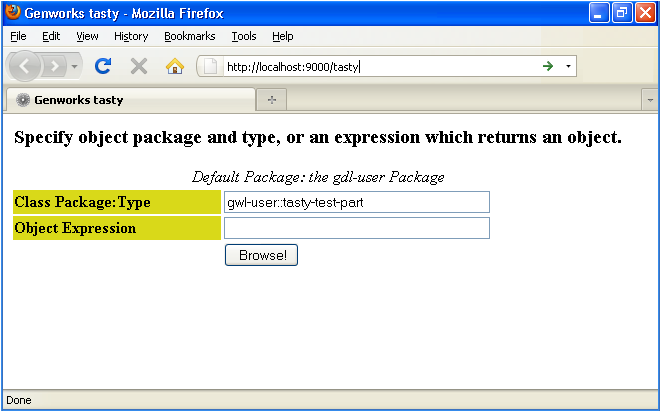
\includegraphics{../images/tasty-start.png}
\end{center}

\caption{Tasty start-up}

\label{fig:tasty-startup}

\end{figure}


Note that if the \texttt{assembly} symbol had not been exported from the \texttt{:chapter-5} package, then a double-colon would have been needed: \texttt{chapter-5::tower1}\footnote{use of a double-colon indicates dubious coding
practice, because it means that the code in quesion is accessing the
``internals'' or ``guts'' of another package, which may not have been
the intent of that other package's designer.}



After you specify the class package and the object type and
press the ``browse'' button, the browser will produce the Tasty
interface with an instance of the specified type (see figure 
\ref{fig:tastytowerpre}). The utility interface
by default is composed of three toolbars and three view frames (tree
frame, inspector frame and viewport frame ``graphical view port'').



\subsection{The Toolbars}

\label{subsec:thetoolbars}



The first toolbar consists of two ``tabs'' which allow the
user to select between the display of the application itself or the
GDL reference documentation.



The second toolbar is designed to select various ``click modes'' for
objects and graphical viewing, and to customize the interface in other
ways. It hosts five menus: edit, tree, view, windows and
help\footnote{A File menu will be added in a future release, to
facilitate saving and restoring of instance ``snapshots'' --- at
present, this can be done programmatically.}.



The \emph{tree menu} allows the user to customize the ``click mode'' of the
mouse (or ``tap mode'' for other pointing devices) for objects in the
tree, inspector, or viewport frames. The behavior follows the \emph{select-and-match} behavior -- you first \emph{select} a mode of operation with one of the buttons or menu items, 
then \emph{match} that mode to any object in the tree frame or inspector frame by
left-clicking (or tapping). These modes are as follows:



\begin{itemize}

\item 
\underline{Tree: Graphical modes}

\begin{description}

\item [Add Node (AN)]
Node in graphics viewport

\item [Add Leaves (AL)]
Add Leaves in graphics viewport

\item [Add Leaves indiv. (AL*)]
Add Leaves individually (so they can be deleted individually).

\item [Draw Node (DN)]
Draw Node in graphics view port (replacing any existing).

\item [Draw Leaves (DL)]
Draw Leaves in graphics view port (replacing any existing).

\item [Clear Leaves (DL)]
Delete Leaves

\end{description}



\item 
\underline{Tree: Inspect \& debug modes}

\begin{description}

\item [Inspect object (I)]
Inspect (make the inspector frame to show the selected object).

\item [Set self to Object (B)]
Sets a global \texttt{self} variable to the selected object, so you can interact by sending messages to the object at the command prompt e.g. by typing \texttt{(the length)} or \texttt{(the children)}.

\item [Set Root to Object (SR)]
Set displayed root in Tasty tree to selected object.

\item [Up Root (UR!)]
Set displayed root in Tasty tree up one level (this is grayed out if already on root).

\item [Reset Root (RR!)]
Reset displayed root in Tasty to to the true root of the tree (this is grayed out if already on root).

\end{description}



\item 
\underline{Tree: frame navigation modes}

\begin{description}

\item [Expand to Leaves (L)]
Nodes expand to their deepest leaves when clicked. 

\item [Expand to Children (C)]
Nodes expand to their direct children when clicked.

\item [Auto Close (A)]
When any node is clicked to expand, all other nodes close automatically.

\item [Remember State (R)]
Nodes expand to their previously expanded state when clicked.

\end{description}



\item 
\underline{View: Viewport Actions}

\begin{description}

\item [Fit to Window!]
Fits to the graphics viewport size the displayed objects (use after a Zoom)

\item [Clear View! (CL!)]
Clear all the objects displayed in the graphics viewport.

\end{description}



\item 
\underline{View: Image Format}

\begin{description}

\item [PNG]
Sets the displayed format in the graphics viewport to PNG (raster image with 
        isoparametric curves for surfaces and brep faces).

\item [JPEG]
Sets the displayed format in the graphics viewport to JPEG
         (raster image with isoparametric curves for surfaces and brep faces).

\item [VRML/X3D]
Sets the displayed format in the graphics viewport to
             VRML with default lighting and viewpoint (these can be changed
             programmatically). This requires a compatible plugin such as BS Contact

\item [X3DOM]
This experimental mode sets the displayed format in the graphics viewport to use the x3dom.js Javascript library,
which attempts to render X3D format directly in-browser without the need for plugins. This works best in WebGL-enabled
browsers such as a recent version of Google Chrome\footnote{Currently, it is necessary to ``Reload'' or
	   ``Refresh'' the browser window to display the geometry in
	   this mode.}.

\item [SVG/VML]
Sets the displayed format in the graphics viewport to SVG/VML\footnote{For complex objects with many display curves,
            SVG/VML can overwhelm the JavaScript engine in the web
            browser. Use PNG for these cases.}, which is a vector graphics image format displaying 
            isoparametric curves for surfaces and brep faces.

\end{description}



\item 
\underline{View: Click Modes}

\begin{description}

\item [Zoom in]
Sets the mouse left-click in the graphics viewport to zoom in.

\item [Zoom out]
Sets the mouse left-click in the graphics viewport to zoom out.

\item [Measure distance]
Calculates the distance between two selected points from the graphics viewport.

\item [Get coordinates]
Displays the coordinates of the selected point from the graphics viewport.

\item [Select Object]
Allows the user to select an object from the graphics
                  viewport (currently works for displayed curves and
                  in SVG/VML mode only).

\end{description}



\item 
\underline{View: Perspective}

\begin{description}

\item [Trimetric]
Sets the displayed perspective in the graphics viewport to trimetric.

\item [Front]
Sets the displayed perspective in the graphics viewport to Front (negative Y axis).

\item [Rear]
Sets the displayed perspective in the graphics viewport to Rear (positive Y axis).

\item [Left]
Sets the displayed perspective in the graphics viewport to Left (negative X axis).

\item [Right]
Sets the displayed perspective in the graphics viewport to Right (positive X axis).

\item [Top]
Sets the displayed perspective in the graphics viewport to Top (positive Z axis).

\item [Bottom]
Sets the displayed perspective in the graphics viewport to Bottom (negative Z axis).

\end{description}



\end{itemize}



The third toolbar hosts the most frequently used
buttons. These buttons have tooltips which will pop up when you hover
the mouse over them. However, these buttons are found in the second
toolbar as well, except for line thickness and color buttons. The line
thickness and color buttons\footnote{The design of the line thickness and color
buttons is being refined and may appear differently in your
installation.} expand and contract when clicked, and allows the user to
select a desired line thickness and color for the objects displayed in
the graphics viewport.



\subsection{View Frames}

\label{subsec:viewframes}



The \emph{tree frame} contains a hierarchical representation of your defined
object. For example for the tower assembly this will be as depicted in
figure 
\ref{fig:tree-twisty-tower}



To draw the graphics (geometry) for the tower leaf-level
objects, you can select the ``Add Leaves (AL)'' item from the Tree
menu, then click the desired leaf to be displayed from the
tree. Alternatively, you can select the ``rapid'' button from the
third toolbar which is symbolized by a pencil icon. Because this
operation (draw leaves) is frequently used, the operation is also
directly available as a direct-click icon which will appear when you
hover the mouse over any leaf or node in the tree.



A direct-click icon is also available for ``inspect
object,'' as the second icon when you hover the mouse over a leaf or
node.



The ``inspector'' frame allows the user to inspect (and in
some cases modify) the object instance being inspected.



For example, we can make the \texttt{number-of-blocks} of the tower to be ``settable,'' by adding the keyword \texttt{:settable} after its default expression (please look ahead to Chapter 
\ref{chap:advancedgendl} if you are interested in more details on this GDL
syntax). We will also pass in the number-of-blocks as the :size of
the \texttt{blocks} sequence, rather than using a hard-coded value as
previously. The new assembly definition is now:

\begin{verbatim};;
	 ;; FLAG -- insert verbatim or ref to new tower code
	 ;; 
\end{verbatim}



In this new version of the tower, the number-of-blocks is a
settable slot, and its value can be modified (i.e. ``bashed'') as
desired, either programmatically from the command-line, in an end-user
application, or from the Tasty environment.



To modify the value in Tasty: select ``Inspect'' mode from the Tree
menu, then select the root of the \texttt{assembly} tree to set the inspector on that object (see Figure 
\ref{fig:tasty-inspector}). Once the inspector is displaying this object, it is
possible to expand its settable slots by clicking on the ``Show
Settables!''  link (use the ``X'' link to collapse the settable slots
view). When the settable slots area is open, the user may set the
values as desired by inputting the new value and pressing the OK
button (see Figure 
\ref{fig:tasty-s-slots}).



\chapter{Working with Geometry in GDL}

\label{chap:workingwithgeometryingdl}



Although Genworks GDL is a powerful framework for a variety
  of general-purpose undertakings, one of its particular strong points
  is generating geometry and processing geometric entities. Geometric
  capabilities are provided by a library of \emph{low-level primitives}, or LLPs. LLPs are pre-defined GDL objects which you can
	extend by ``mixing in'' with your own definitions, and/or
	instantiate as child objects in your definitions.



The names of the geometric LLPs are in the \texttt{:geom-base} package, and here are some examples:

\begin{itemize}

\item \texttt{base-coordinate-system} provides an empty 3D Cartesian coordinate system.\footnote{\texttt{base-coordinate-system} is also known by its legacy name \texttt{base-object}}

\item Simple 2-dimensional primitives include \texttt{line}, \texttt{arc}, and \texttt{ellipse}.

\item Simple 3-dimensional primitives include \texttt{box}, \texttt{sphere}, and \texttt{cylinder}.

\item Advanced 3-dimensional primitives (which depend on optional add-on Geometry Kernel module) include \texttt{b-spline-curve}, \texttt{b-spline-surface}, and \texttt{merged-solid}.

\end{itemize}

This chapter will cover the default coordinate system of GDL as well as the built-in simple 2D and 3D LLPs. Chapter 
\ref{chap:workingwithsurfacesandsolids} will cover the advanced Surfaces and Solids primitives.



\section{The Default Coordinate System in GDL}

\label{sec:thedefaultcoordinatesystemingdl}



GDL's default coordinate system comes with the standard mixin \texttt{base-coordinate-system} and represents a standard three-dimensional Cartesian
	 Coordinate system with X, Y, and Z dimensions.


\begin{figure}
\begin{center}
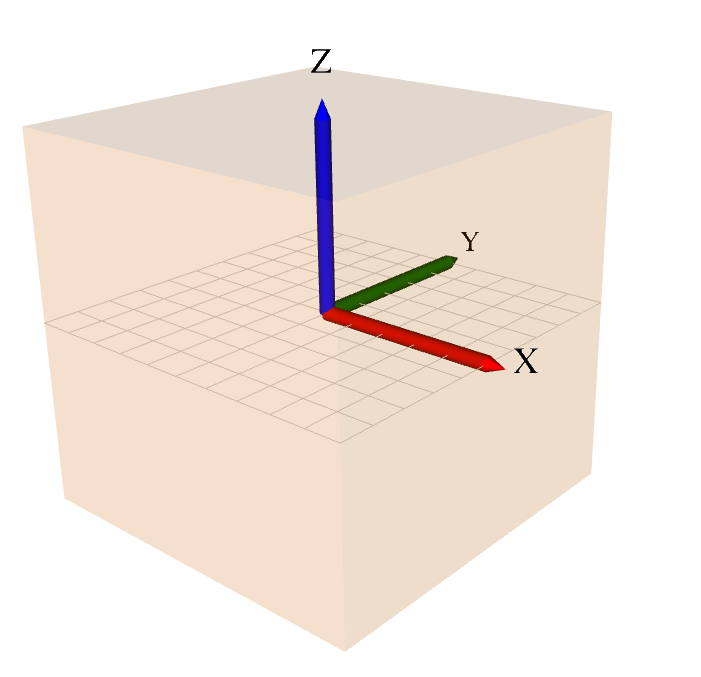
\includegraphics[width=3in,height=3in]{../images/coord-sys-tri.png}
\end{center}

\caption{Coordinate System in Trimetric View}

\label{fig:coord-sys-tri}

\end{figure}

\begin{figure}
\begin{center}
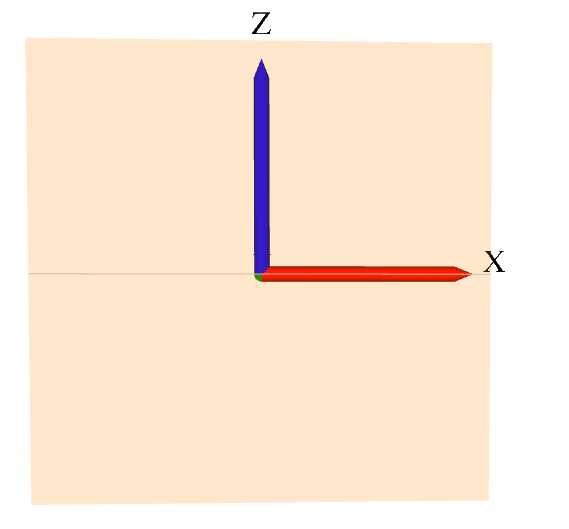
\includegraphics[width=3in,height=3in]{../images/coord-sys-front.png}
\end{center}

\caption{Coordinate System in Front View}

\label{fig:coord-sys-front}

\end{figure}

\begin{figure}
\begin{center}
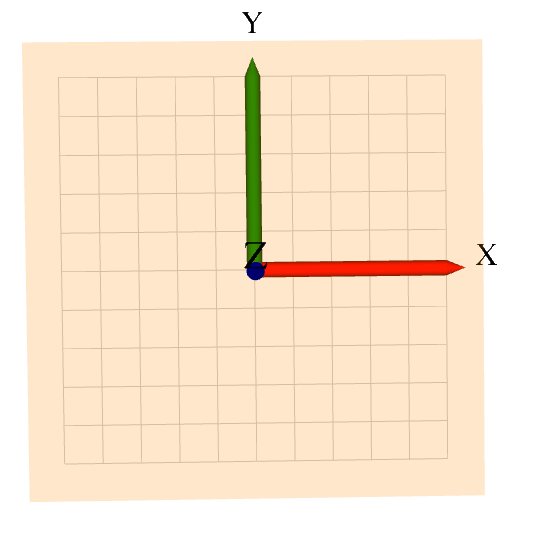
\includegraphics[width=3in,height=3in]{../images/coord-sys-top.png}
\end{center}

\caption{Coordinate System in Top View}

\label{fig:coord-sys-top}

\end{figure}

\begin{figure}
\begin{center}
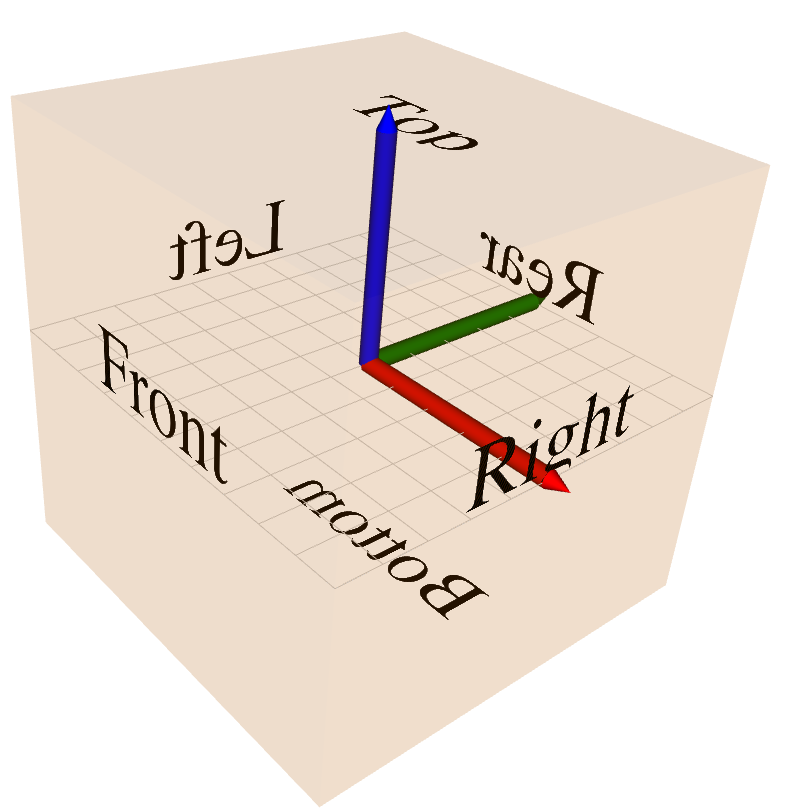
\includegraphics[width=3in,height=3in]{../images/coord-sys-labeled-faces.png}
\end{center}

\caption{Coordinate System with Symbolically Labeled Faces}

\label{fig:coord-sys-labeled-faces}

\end{figure}


Figure 
\ref{fig:coord-sys-tri} shows the coordinate system in a 3D Trimetric view.



Figure 
\ref{fig:coord-sys-front} shows the coordinate system in a Front View.



Figure 
\ref{fig:coord-sys-top} shows the coordinate system in a Top View.



Figure 
\ref{fig:coord-sys-labeled-faces} shows each face of the reference box labeled with its symbolic direction:

\begin{itemize}

\item \texttt{Right} for the 
\textbf{positive X} direction

\item \texttt{Left} for the 
\textbf{negative X} direction

\item \texttt{Rear} for the 
\textbf{positive Y} direction

\item \texttt{Front} for the 
\textbf{negative Y} direction

\item \texttt{Top} for the 
\textbf{positive Z} direction

\item \texttt{Bottom} for the 
\textbf{negative Z} direction

\end{itemize}





\section{Building a Geometric GDL Model from LLPs}

\label{sec:buildingageometricgdlmodelfromllps}

The simplest geometric entity in GDL is a \texttt{box}, and in fact all entities are associated with an imaginary \emph{reference box} which shares the same slots as a normal box. The \texttt{box} primitive type in GDL inherits its inputs from \texttt{base-coordinate-system}, and the fundamental inputs are:

\begin{itemize}

\item \texttt{center} Default: \texttt{\#(0.0 0.0 0.0)}

\item \texttt{orientation} Default: \texttt{nil}

\item \texttt{height} Default: \texttt{0}

\item \texttt{length} Default: \texttt{0}

\item \texttt{width} Default: \texttt{0}

\end{itemize}



Figure 
\ref{fig:box-code} defines an example box, and Figure 
\ref{fig:tasty-box} demonstrates how it will display in Tasty.



Note the following from the example in 
\ref{fig:box-code}:

\begin{itemize}

\item The symbol \texttt{+phi+}\footnote{By convention, constants in Common Lisp are
	    named with a leading and trailing \texttt{+} as a way to make them recognizable as constants.} holds a global constant containing the ``golden ratio''
	    number, which is approximated as 1.618.

\item The slots \texttt{length}, \texttt{width}, and \texttt{height}
 are defined in \texttt{base-object} as \emph{trickle-down-slots}. For this reason they are automatically being passed down
into into the \texttt{box} child object. Therefore it is not necessary to pass them down explicitly.
\end{itemize}




\begin{figure}
\begin{lrbox}{\boxedverb}
\begin{minipage}{\linewidth}

\begin{verbatim}(in-package :gdl-user)

(define-object box-assembly-1 (base-object)

  :computed-slots ((length 10)
                   (width (* (the length) +phi+))
                   (height (* (the width) +phi+)))
  :objects ((box :type 'box)))
                 

\end{verbatim}
\end{minipage}
\end{lrbox}
\fbox{\usebox{\boxedverb}}

\caption{Definition of a Box}

\label{fig:box-code}

\end{figure}

\begin{figure}
\begin{center}
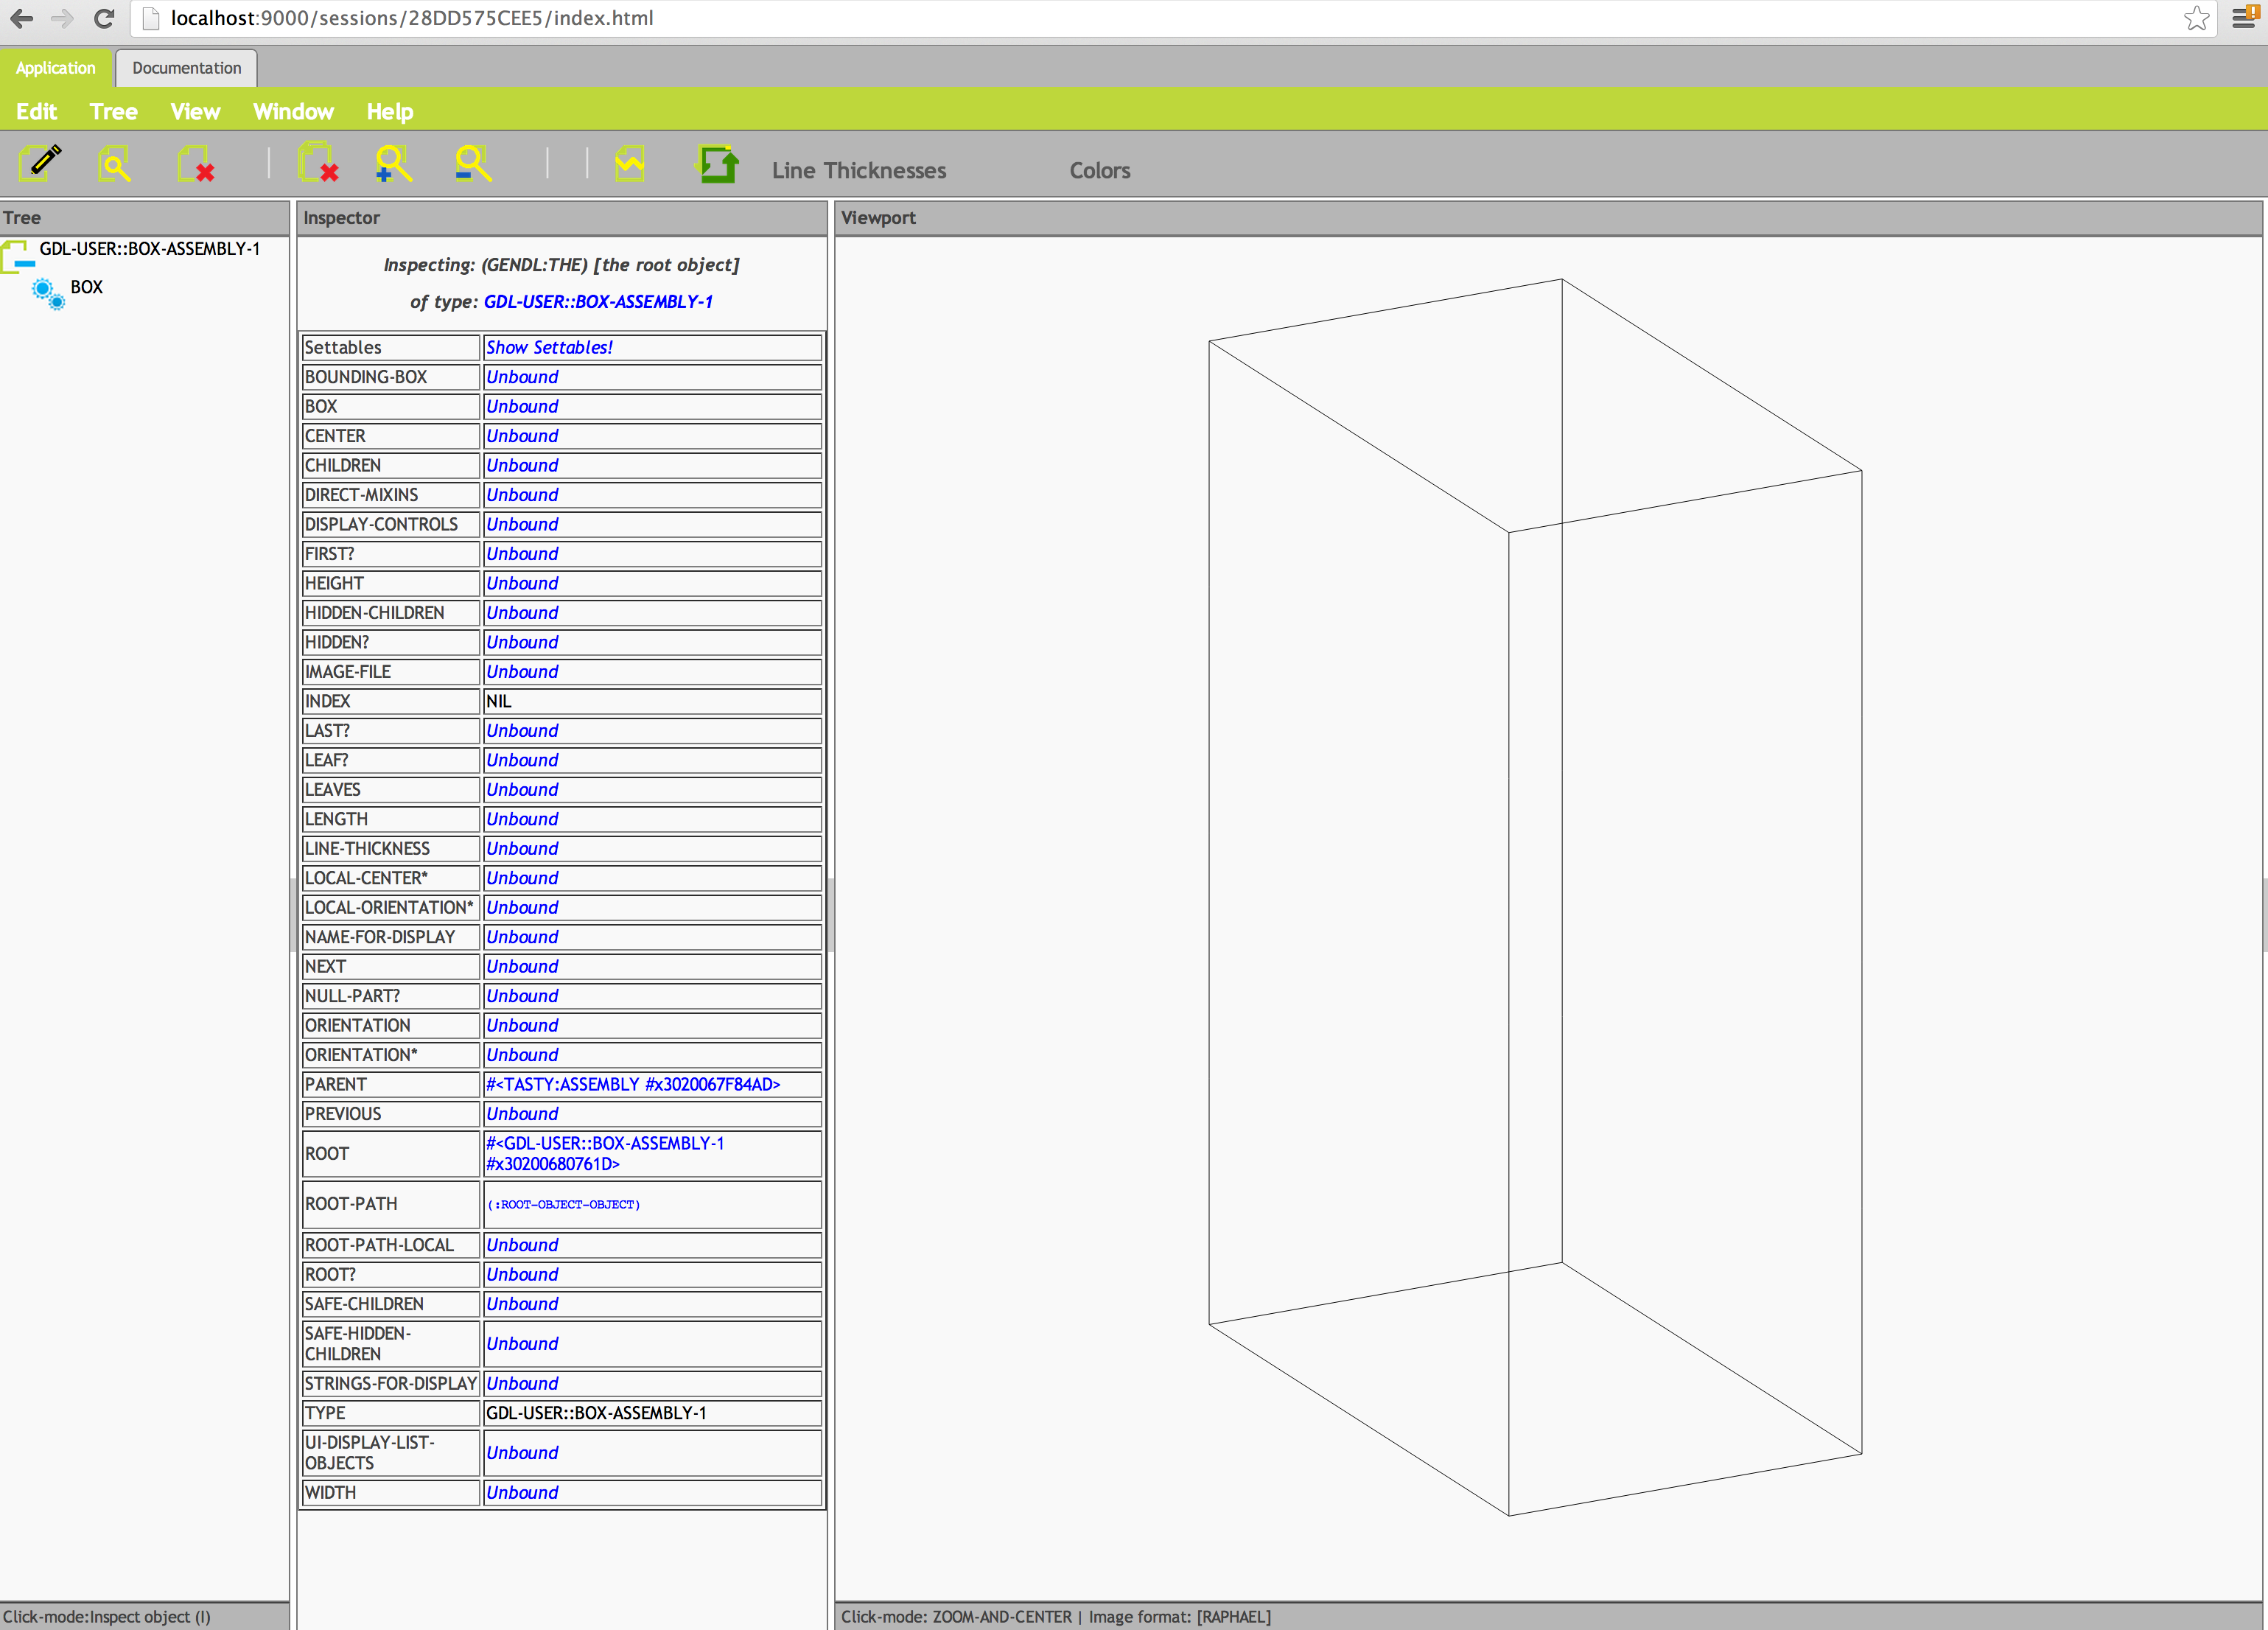
\includegraphics[width=4in,height=3in]{../images/tasty-box-1.png}
\end{center}

\caption{Simple box displayed in Tasty}

\label{fig:tasty-box}

\end{figure}


\subsection{Positioning a child object using the center input}

\label{subsec:positioningachildobjectusingthecenterinput}

\begin{figure}\begin{lrbox}{\boxedverb}
\begin{minipage}{\linewidth}\begin{verbatim}(in-package :gdl-user)

(define-object positioned-boxes (base-object)

  :computed-slots ((length 10)
                   (width (* (the length) +phi+))
                   (height (* (the width) +phi+)))

  :objects ((box-1 :type 'box)
            (box-2 :type 'box 
                   :center (make-point (the width)  0 0))))
            
                 

\end{verbatim}\end{minipage}
\end{lrbox}
\fbox{\usebox{\boxedverb}}

\caption{Positioned Boxes source}

\label{fig:positioned-boxes-source}

\end{figure}

\begin{figure}
\begin{center}
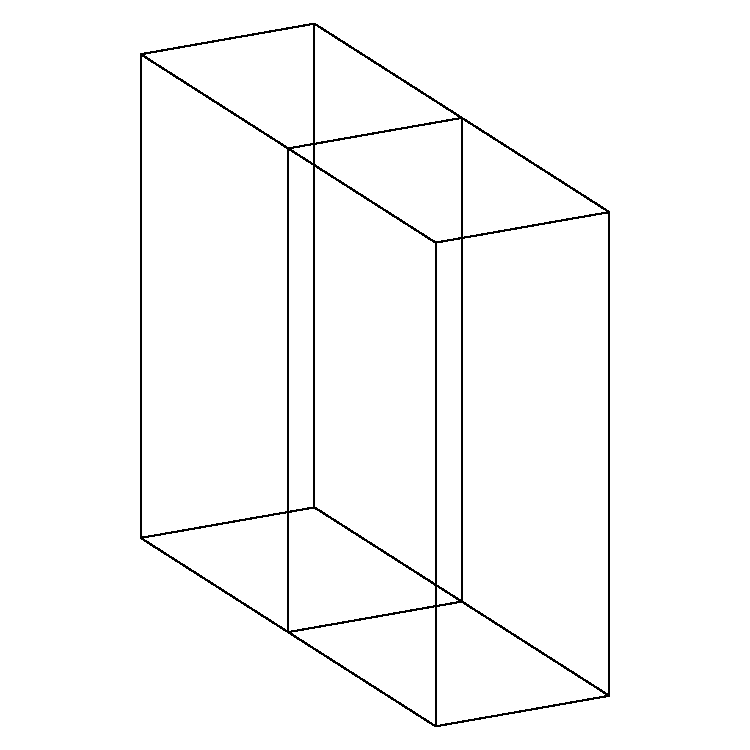
\includegraphics[width=4in,height=4in]{../images/positioned-boxes.pdf}
\end{center}

\caption{Positioned Boxes}

\label{fig:positioned-boxes}

\end{figure}


By default, a child object will be positioned at the same \texttt{center} as its parent, and the \texttt{center} defaults to the point \texttt{\#(0.0 0.0 0.0)}. Figure 
\ref{fig:positioned-boxes-source} (rendered in Figure 
\ref{fig:positioned-boxes}) shows a second box being positioned adjacent to the first, by using the \texttt{:center} input. 



\subsection{Positioning Sequence Elements using (the-child index)}

\label{subsec:positioningsequenceelementsusing(the-childindex)}

When specifying a sequence of child objects, each individual sequence element
can be referenced from within its \texttt{:objects} section using the operator \texttt{the-child}. By using \texttt{the-child} to send the \texttt{index} message, you can obtain the index\footnote{Indices in GDL ``size'' sequences are integers which start with 0 (zero).} of each individual child object as it is being processed. 
In this manner it is possible to compute a distinct position for each child, as a function of its
index, as demonstrated in Figures 
\ref{fig:positioned-by-index-source} and 
\ref{fig:positioned-by-index}.\begin{figure}\begin{lrbox}{\boxedverb}
\begin{minipage}{\linewidth}\begin{verbatim}(in-package :gdl-user)

(define-object positioned-by-index (base-object)
  
  :input-slots ((number-of-boxes 5))

  :computed-slots ((length 10)
                   (width (* (the length) +phi+))
                   (height (* (the width) +phi+)))

  :objects ((boxes :type 'box
                   :sequence (:size (the number-of-boxes))
                   :center (make-point (* (the width) (the-child index))
                                       0 0))))
            
                 

\end{verbatim}\end{minipage}
\end{lrbox}
\fbox{\usebox{\boxedverb}}

\caption{Positioned by Index source}

\label{fig:positioned-by-index-source}

\end{figure}

\begin{figure}
\begin{center}
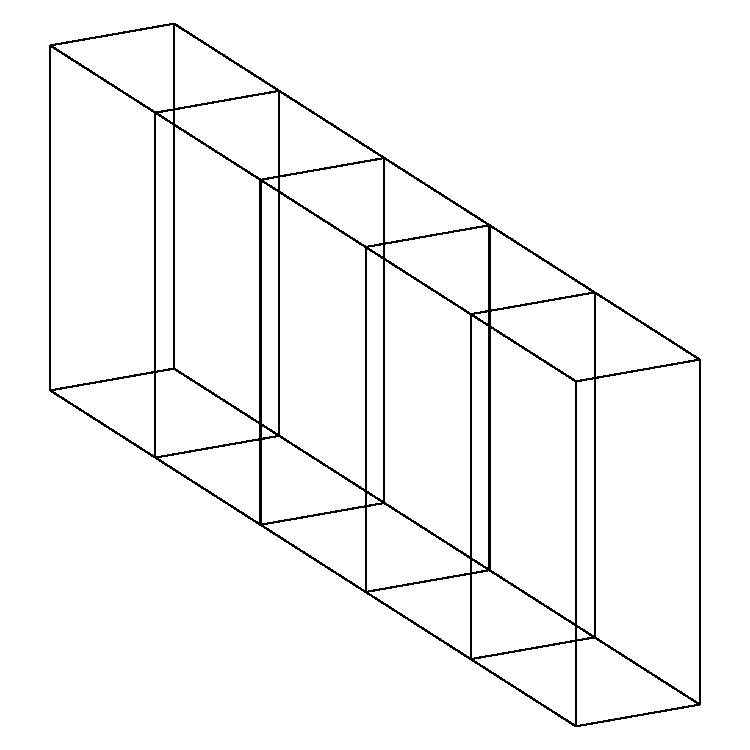
\includegraphics[width=4in,height=4in]{../images/positioned-by-index.pdf}
\end{center}

\caption{Positioned by Index}

\label{fig:positioned-by-index}

\end{figure}


\subsection{Relative positioning using the translate operator}

\label{subsec:relativepositioningusingthetranslateoperator}



It is usually preferable to position child objects in a \emph{relative} rather than \emph{absolute} manner with respect to the parent. For example, in our positioned-by-index example in Figure 
\ref{fig:positioned-by-index-source}, each child box object is being positioned using an absolute coordinate produced by \texttt{make-point}. This will work as long as the center of the current parent is \texttt{\#(0.0 0.0 0.0)} (which it is, by default). But imagine if this parent
     itself is a child of a larger assembly. Imagine further that the
     larger assembly specifies a non-default center for this instance
     of \texttt{positioned-by-index}. At this point, the strategy fails.



The solution is to adhere to a consistent Best Practice of positioning child objects according to the \texttt{center} (or some other known datum point) of the parent
	 object. This can easily be accomplished through the use of
	 the \emph{translate} operator. The \texttt{translate} operator works within the context of a GDL object, and
	 allows a 3D point to be translated in up to three directions, selected from: \texttt{:up}, \texttt{:down}, \texttt{:left}, \texttt{:right}, \texttt{:front}, \texttt{:rear}. Figures 
\ref{fig:translate-by-index-source} and 
\ref{fig:translate-by-index} show the equivalent of our positioned-by-index example, but
with all the positioning done relative to the parent's center.\begin{figure}\begin{lrbox}{\boxedverb}
\begin{minipage}{\linewidth}\begin{verbatim}(in-package :gdl-user)

(define-object translate-by-index (base-object)
  
  :input-slots ((number-of-boxes 5))

  :computed-slots ((length 10)
                   (width (* (the length) +phi+))
                   (height (* (the width) +phi+)))

  :objects ((boxes :type 'box
                   :sequence (:size (the number-of-boxes))
                   :center (translate (the center) 
                                      :right (* (the width) (the-child index))))))
            
                 

\end{verbatim}\end{minipage}
\end{lrbox}
\fbox{\usebox{\boxedverb}}

\caption{Translated by Index source}

\label{fig:translate-by-index-source}

\end{figure}

\begin{figure}
\begin{center}
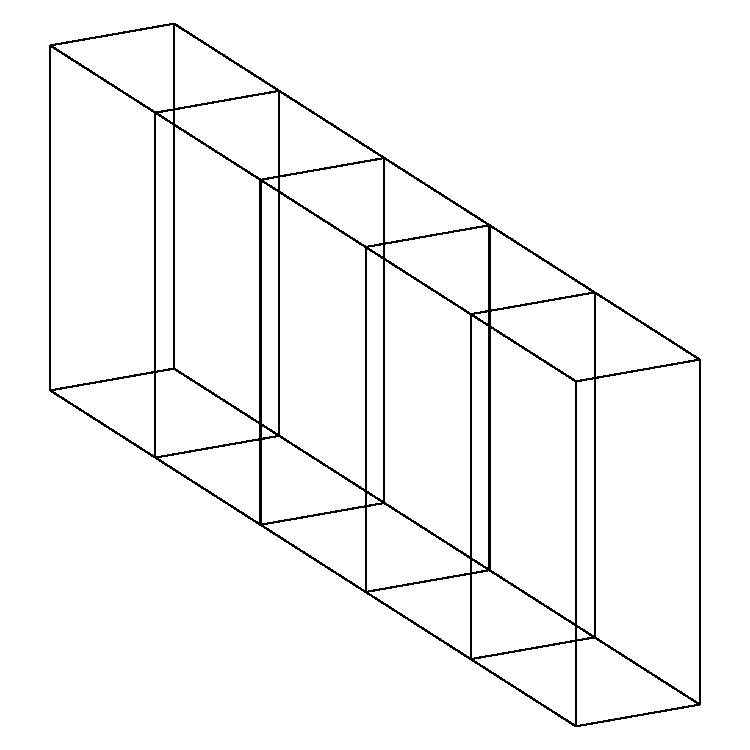
\includegraphics[width=4in,height=4in]{../images/translate-by-index.pdf}
\end{center}

\caption{Translated by Index}

\label{fig:translate-by-index}

\end{figure}




\subsection{Display Controls}

\label{subsec:displaycontrols}



It is possible to specify particular default display
	 characteristics\footnote{In addition to display-controls attached to a geometric entity 
itself, GDL also supports the concept of \emph{lenses}, which capture the program code used to output a
		    particular class of  entities (e.g. \texttt{box} in a particular output format (e.g. \texttt{pdf}. Lenses will be covered in more detail in Chapter 
\ref{chap:input-output}.} for objects in GDL, such as: 

\begin{itemize}

\item color

\item line-thickness (for line-based output formats like PDF)

\item transparency (for shaded graphics outputs like X3D)

\end{itemize}





The most common display-control is probably \texttt{:color}. Color in GDL can be specified in one of three formats:
\begin{figure}
\begin{center}
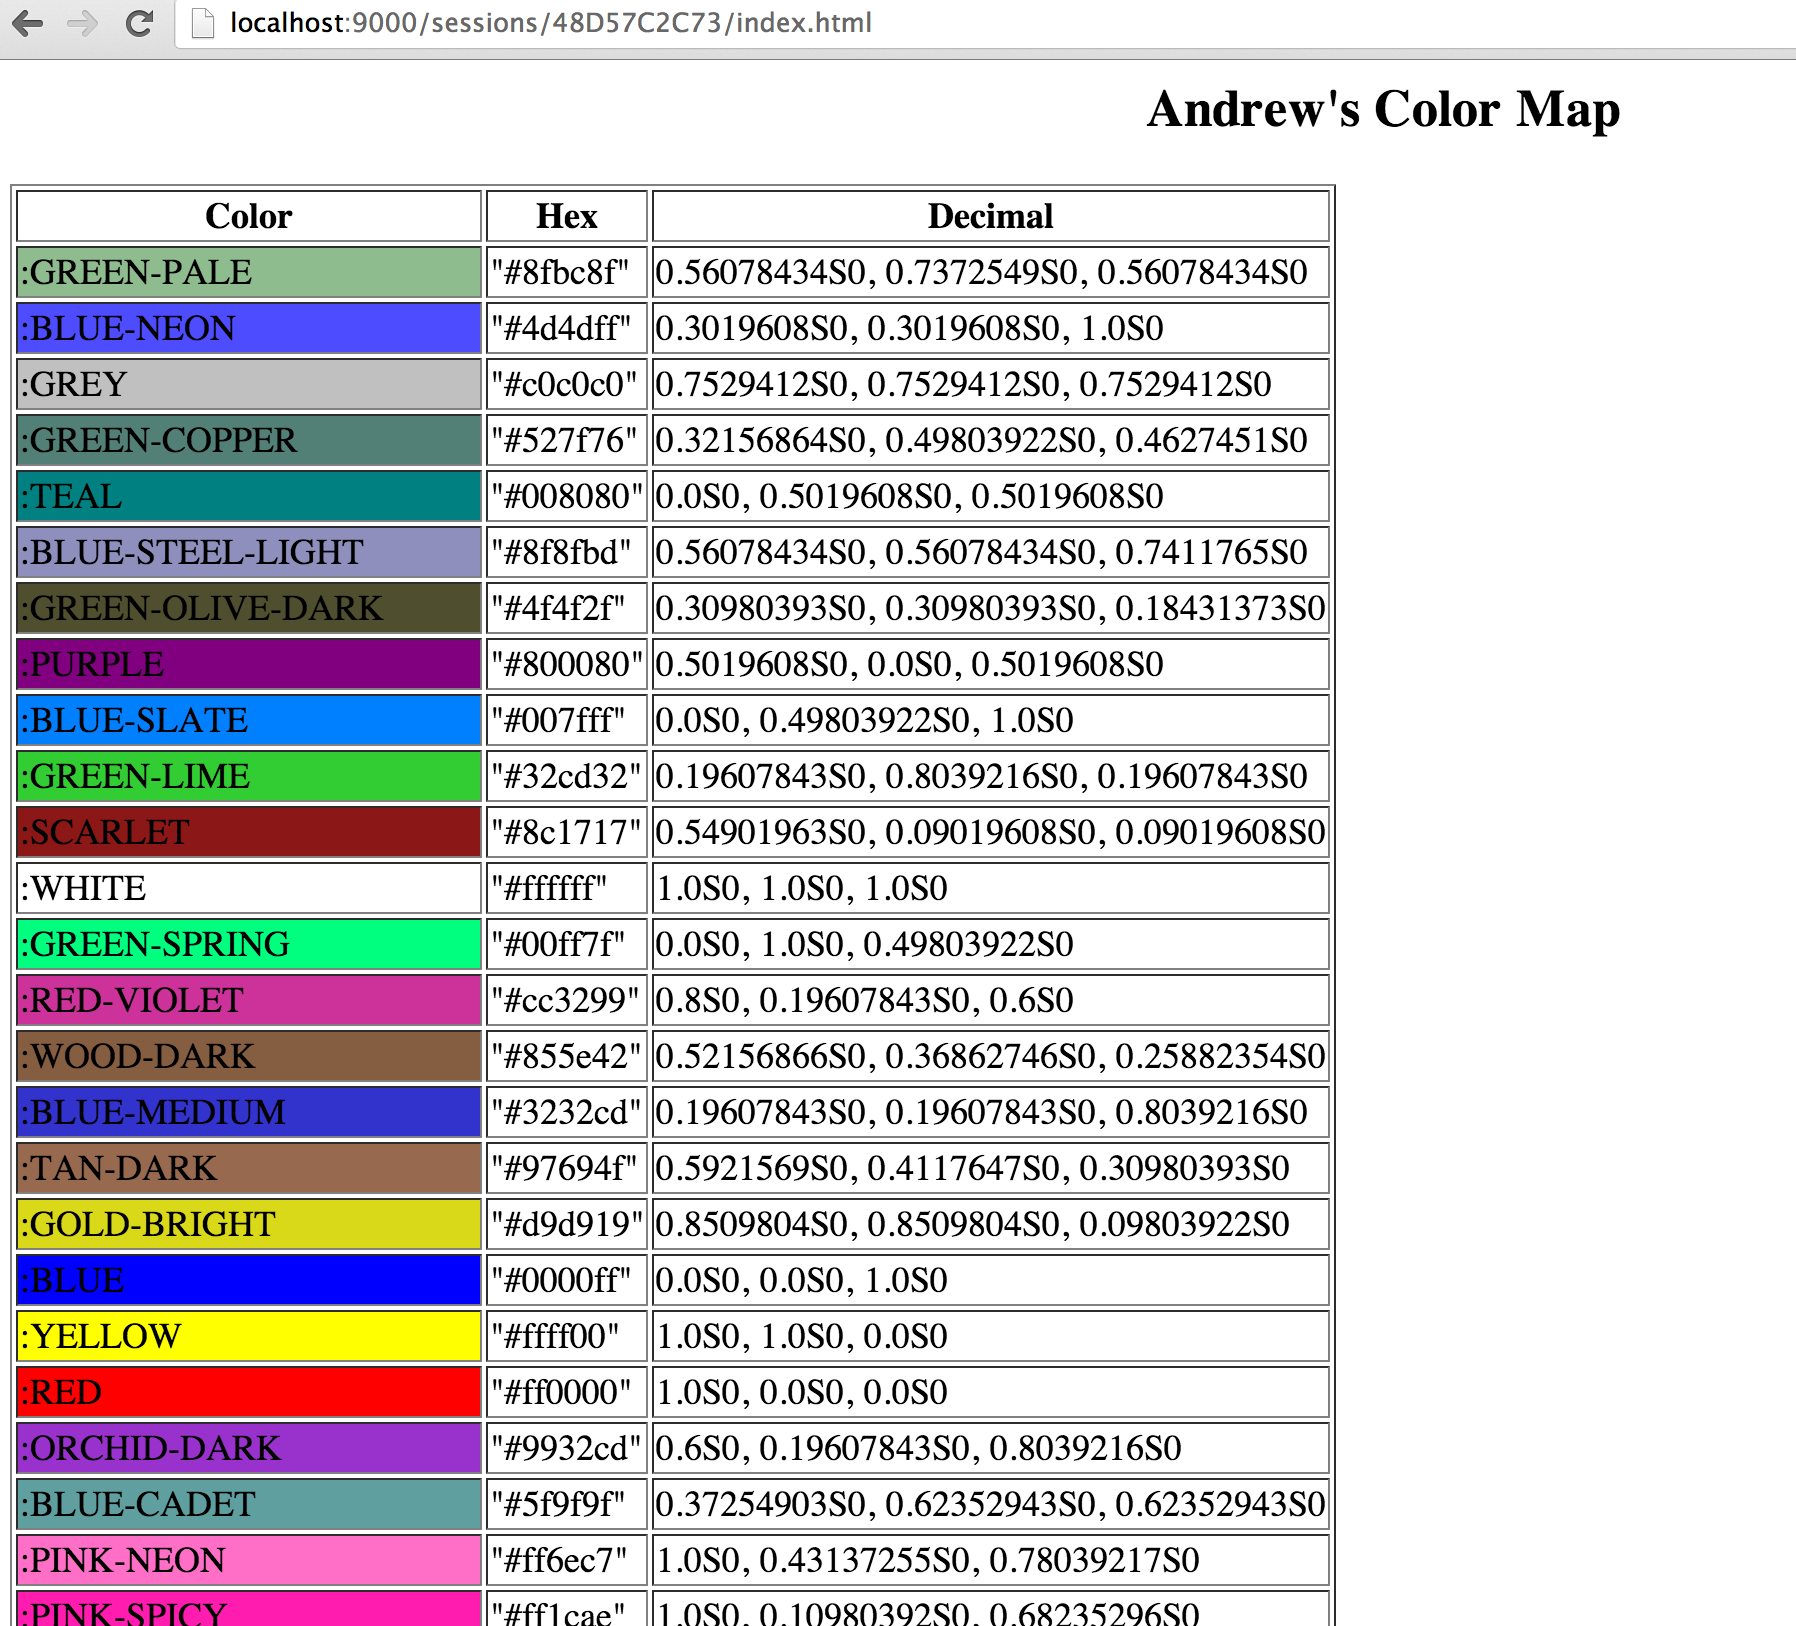
\includegraphics{../images/color-map.png}
\end{center}

\caption{Color Map (assembled by Andrew
			 Wolven from standard X Window colors)}

\label{fig:color-map}

\end{figure}


\begin{enumerate}

\item By name. The names can be seen at the URL \texttt{http://localhost:9000/color-map} as seen in Figure 
\ref{fig:color-map}

\item By hexadecimal Red-Green-Blue values, in the form of
	  a string beginning with the ``\#'' character. Each two-digit
	  hex number represents a component of Red, Green, or Blue (to
	  make this easy to remember, use the mnemonic ``Roy G. Biv''
	  from the rainbow colors). For example, \texttt{\#000000} represents pure Black, and \texttt{\#FFFFFF} represents pure White. \texttt{\#FF0000} would be pure Red, \texttt{\#00FF00} would be pure Green, and \texttt{\#FF00FF} would be Purple (a mix of Red and Blue). Note that this
	    is also a standard for HTML and the World Wide Web.

\item By a list of three decimal numbers between 0.0 and
	  1.0, again representing values for Red, Green, and Blue. For example, \texttt{(1.0 1.0 1.0)} would be pure White, and \texttt{(0.0 0.0 0.0)} would be pure Black.

\end{enumerate}

 The \texttt{display-controls} is an optional input-slot for any geometric entity in GDL,
and is expected to be a \emph{Property List} containing alternating keywords and values. Common keywords for the \texttt{display-controls}, corresponding to the display characteristics listed above, are: 

\begin{itemize}

\item \texttt{:color}

\item \texttt{:line-thickness}

\item \texttt{:transparency}

\end{itemize}

 Figures 
\ref{fig:display-color} and 
\ref{fig:display-color-source} demonstrate the use of the \texttt{:color} keyword in the \texttt{display-controls} for our positioned boxes example.

\begin{figure}\begin{lrbox}{\boxedverb}
\begin{minipage}{\linewidth}\begin{verbatim}(in-package :gdl-user)

(define-object display-color (base-object)
  
  :input-slots ((number-of-boxes 5))

  :computed-slots ((length 10)
                   (width (* (the length) +phi+))
                   (height (* (the width) +phi+))
                   
                   (color-list (list :red :orange :yellow :blue :indigo :violet)))

  :objects ((boxes :type 'box
                   :sequence (:size (the number-of-boxes))
                   :display-controls (list :color (or (nth (the-child index)
                                                           (the color-list)) :black)
                                           :line-thickness 2)
                   :center (translate (the center) 
                                      :right (* (the width) (the-child index))))))
            
                 

\end{verbatim}\end{minipage}
\end{lrbox}
\fbox{\usebox{\boxedverb}}

\caption{Color controlled by display-controls source}

\label{fig:display-color-source}

\end{figure}

\begin{figure}
\begin{center}
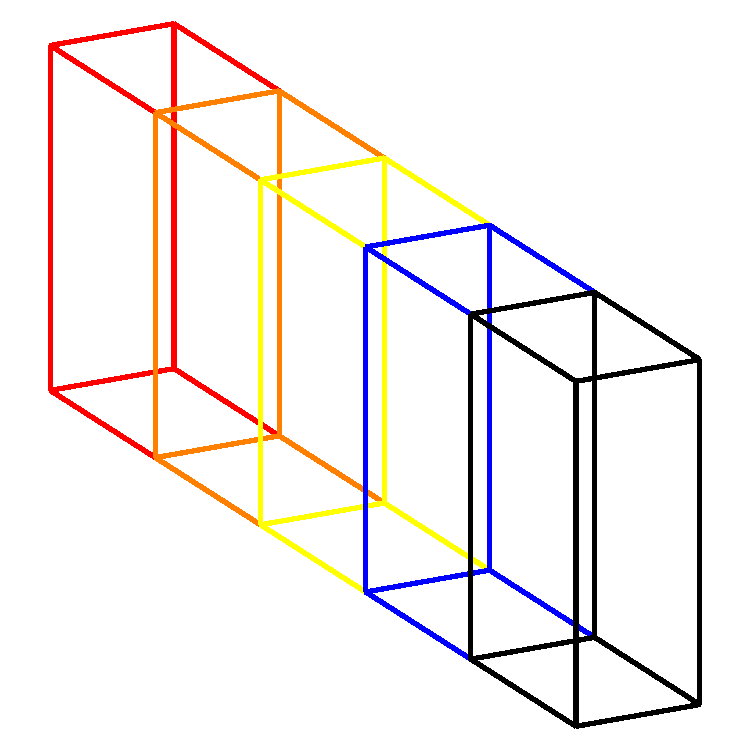
\includegraphics[width=4in,height=4in]{../images/display-color.pdf}
\end{center}

\caption{Color controlled by display-controls}

\label{fig:display-color}

\end{figure}


\subsection{Orientation and the Alignment function}

\label{subsec:orientationandthealignmentfunction}



Orientations in GDL are specified using a 3x3 orientation
matrix. The simplest way to compute an orientation matrix is to use
the use the \texttt{alignment} function. The \texttt{alignment} function accepts up to three direction keywords, and
corresponding vectors to which these directions should be aligned. For
example, to obtain an orientation matrix specifying that the Rear of a
reference box should be aligned with the vector \texttt{\#(1.0 0.0 0.0)}, you could call 

\begin{verbatim}(alignment :rear (make-vector 1 0 0))
\end{verbatim}

\begin{figure}\begin{lrbox}{\boxedverb}
\begin{minipage}{\linewidth}\begin{verbatim}(in-package :gdl-user)

(define-object vertical-cylinder (base-object)

  :objects
  ((horizontal-cylinder :type 'cylinder
                        :display-controls (list :color :green)
                        :length 10 :radius 3)

   (vertical-cylinder :type 'cylinder
                      :length 10 :radius 3
                      :display-controls (list :color :red)
                      :orientation (alignment :rear 
                                              (the (face-normal-vector :top))))))

\end{verbatim}\end{minipage}
\end{lrbox}
\fbox{\usebox{\boxedverb}}

\caption{Cylinder aligned vertically source}

\label{fig:vertical-cylinder-source}

\end{figure}

\begin{figure}
\begin{center}
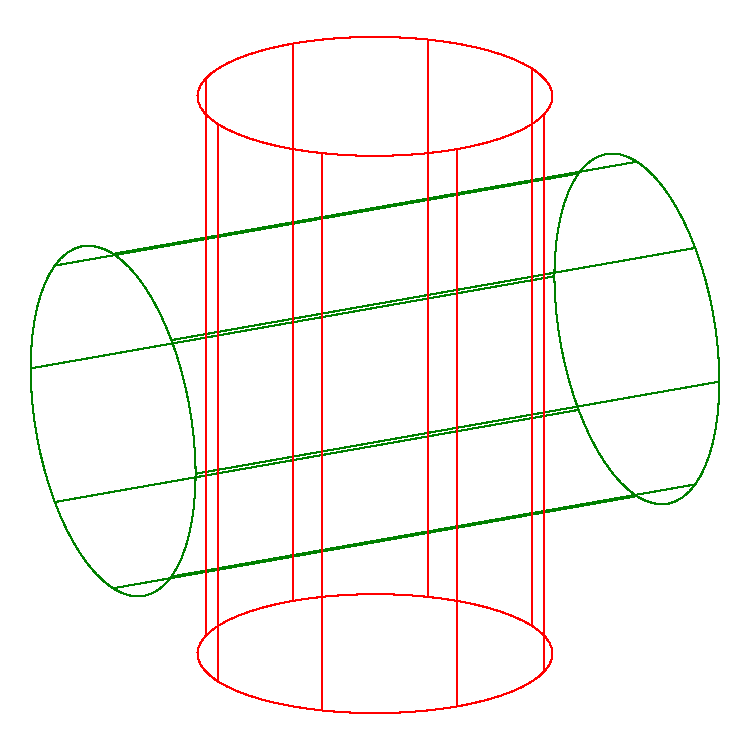
\includegraphics[width=4in,height=4in]{../images/vertical-cylinder.pdf}
\end{center}

\caption{Cylinder aligned vertically}

\label{fig:vertical-cylinder}

\end{figure}


Generally, you will want the orientation of a child object to be 
specified in a \emph{relative} manner to that of the current (parent) object. The concept here is 
similar to that for positioning with respect to \texttt{(the center)}. For relative orientation, you can utilize the various \texttt{face-normal-vector}s of the parent object. For example, by default, cylinders are aligned with 
their flat ends along the longitudinal (Y) axis. Figures 
\ref{fig:vertical-cylinder-source} and 
\ref{fig:vertical-cylinder} show the red cylinder which is turned to be
	 vertical (aligned to the Z axis), by aligning its \texttt{:rear} face with \texttt{(the (face-normal-vector :top))} of the parent base-object.

\begin{figure}\begin{lrbox}{\boxedverb}
\begin{minipage}{\linewidth}\begin{verbatim}(in-package :gdl-user)

(define-object tower (base-object)
  :input-slots 
  ((height 42)
   (block-height 1)
   (width +phi+)
   (length (* (the width) +phi+)))

  :computed-slots
  ((number-of-blocks (floor (the height)
                            (the block-height))))

  :objects
  ((blocks :type 'box
           :sequence (:size (the number-of-blocks))
           :length (the length)
           :height (the block-height)
           :width (the width)
           :center (translate (the center) :up 
                              (* (the-child height)
                                 (the-child index)))
           :orientation (alignment :rear (rotate-vector-d 
                                          (the (face-normal-vector :rear))
                                          (twice (the-child index))
                                          (the (face-normal-vector :top)))))))

\end{verbatim}\end{minipage}
\end{lrbox}
\fbox{\usebox{\boxedverb}}

\caption{Twisty Tower  source}

\label{fig:tower-source}

\end{figure}

\begin{figure}
\begin{center}
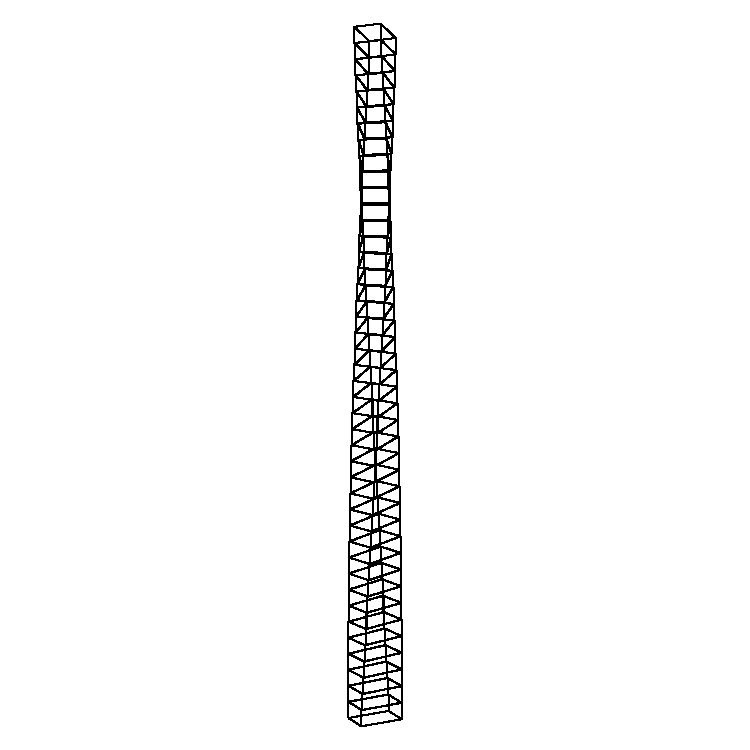
\includegraphics[width=4in,height=4in]{../images/tower.pdf}
\end{center}

\caption{Twisty Tower }

\label{fig:tower}

\end{figure}


\subsection{Rotating vectors with the rotate-vector-d function}

\label{subsec:rotatingvectorswiththerotate-vector-dfunction}

In order to specify a vector which is not aligned exactly with
one of the major axes, you can use the \texttt{rotate-vector-d} function to yield a new vector which is the result of
     ``rotating'' one vector about another vector. Figures 
\ref{fig:tower-source} and 
\ref{fig:tower} show a stack of boxes, where the rear face of each box is
     rotated 2 degrees with respect to the box under it.

\subsection{Assemblies}

\label{subsec:assemblies}

Objects which you define with \texttt{define-object} can be used no differently from the built-in primitives. This
underscores why it is important for the positioning and orientation
passed into a child object be \emph{relative} to that present in the parent. Figures 
\ref{fig:tower-assembly} and 
\ref{fig:tower-assembly-source} show how several towers can be positioned side-by-side, while
maintaining consistent internal positioning and orientation. Figure 
\ref{fig:tower-assembly-tasty} shows how the child towers form an \emph{assembly hierarchy} of objects.\begin{figure}\begin{lrbox}{\boxedverb}
\begin{minipage}{\linewidth}\begin{verbatim}(in-package :gdl-user)

(define-object tower-assembly (base-object)
  :input-slots 
  ((base-height 10)
   (height-deviation 5)
   (number-of-towers 5))
  
  
  :objects
  ((towers :type 'tower
           :sequence (:size (the number-of-towers))
           :height (+ (* (the-child index) (the height-deviation))
		      (the base-height))
           :center (translate (the center) :right (* (twice
						      (twice (the-child width)))
						     (the-child index))))))

 

\end{verbatim}\end{minipage}
\end{lrbox}
\fbox{\usebox{\boxedverb}}

\caption{Tower Assembly source}

\label{fig:tower-assembly-source}

\end{figure}

\begin{figure}
\begin{center}
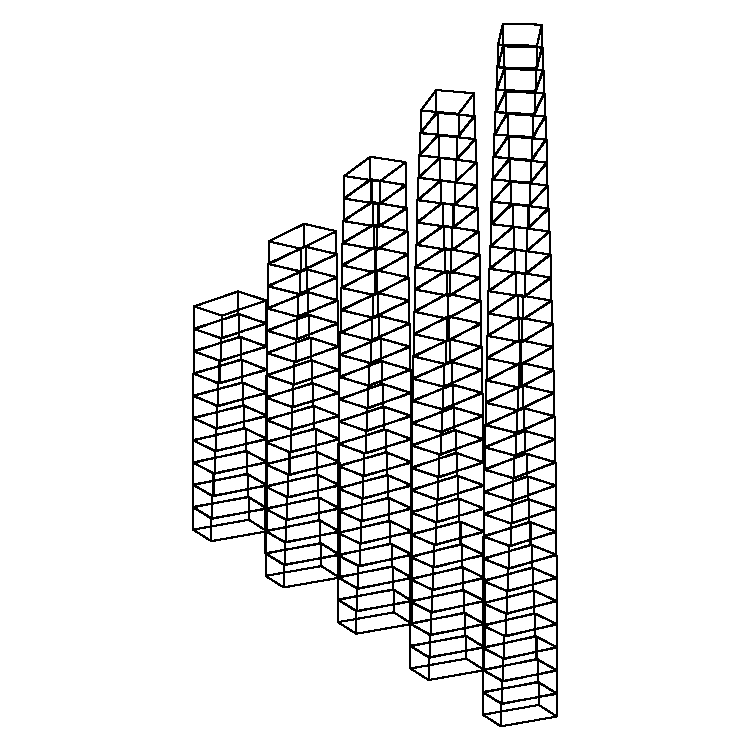
\includegraphics[width=4in,height=4in]{../images/tower-assembly.pdf}
\end{center}

\caption{Tower Assembly}

\label{fig:tower-assembly}

\end{figure}

\begin{figure}
\begin{center}
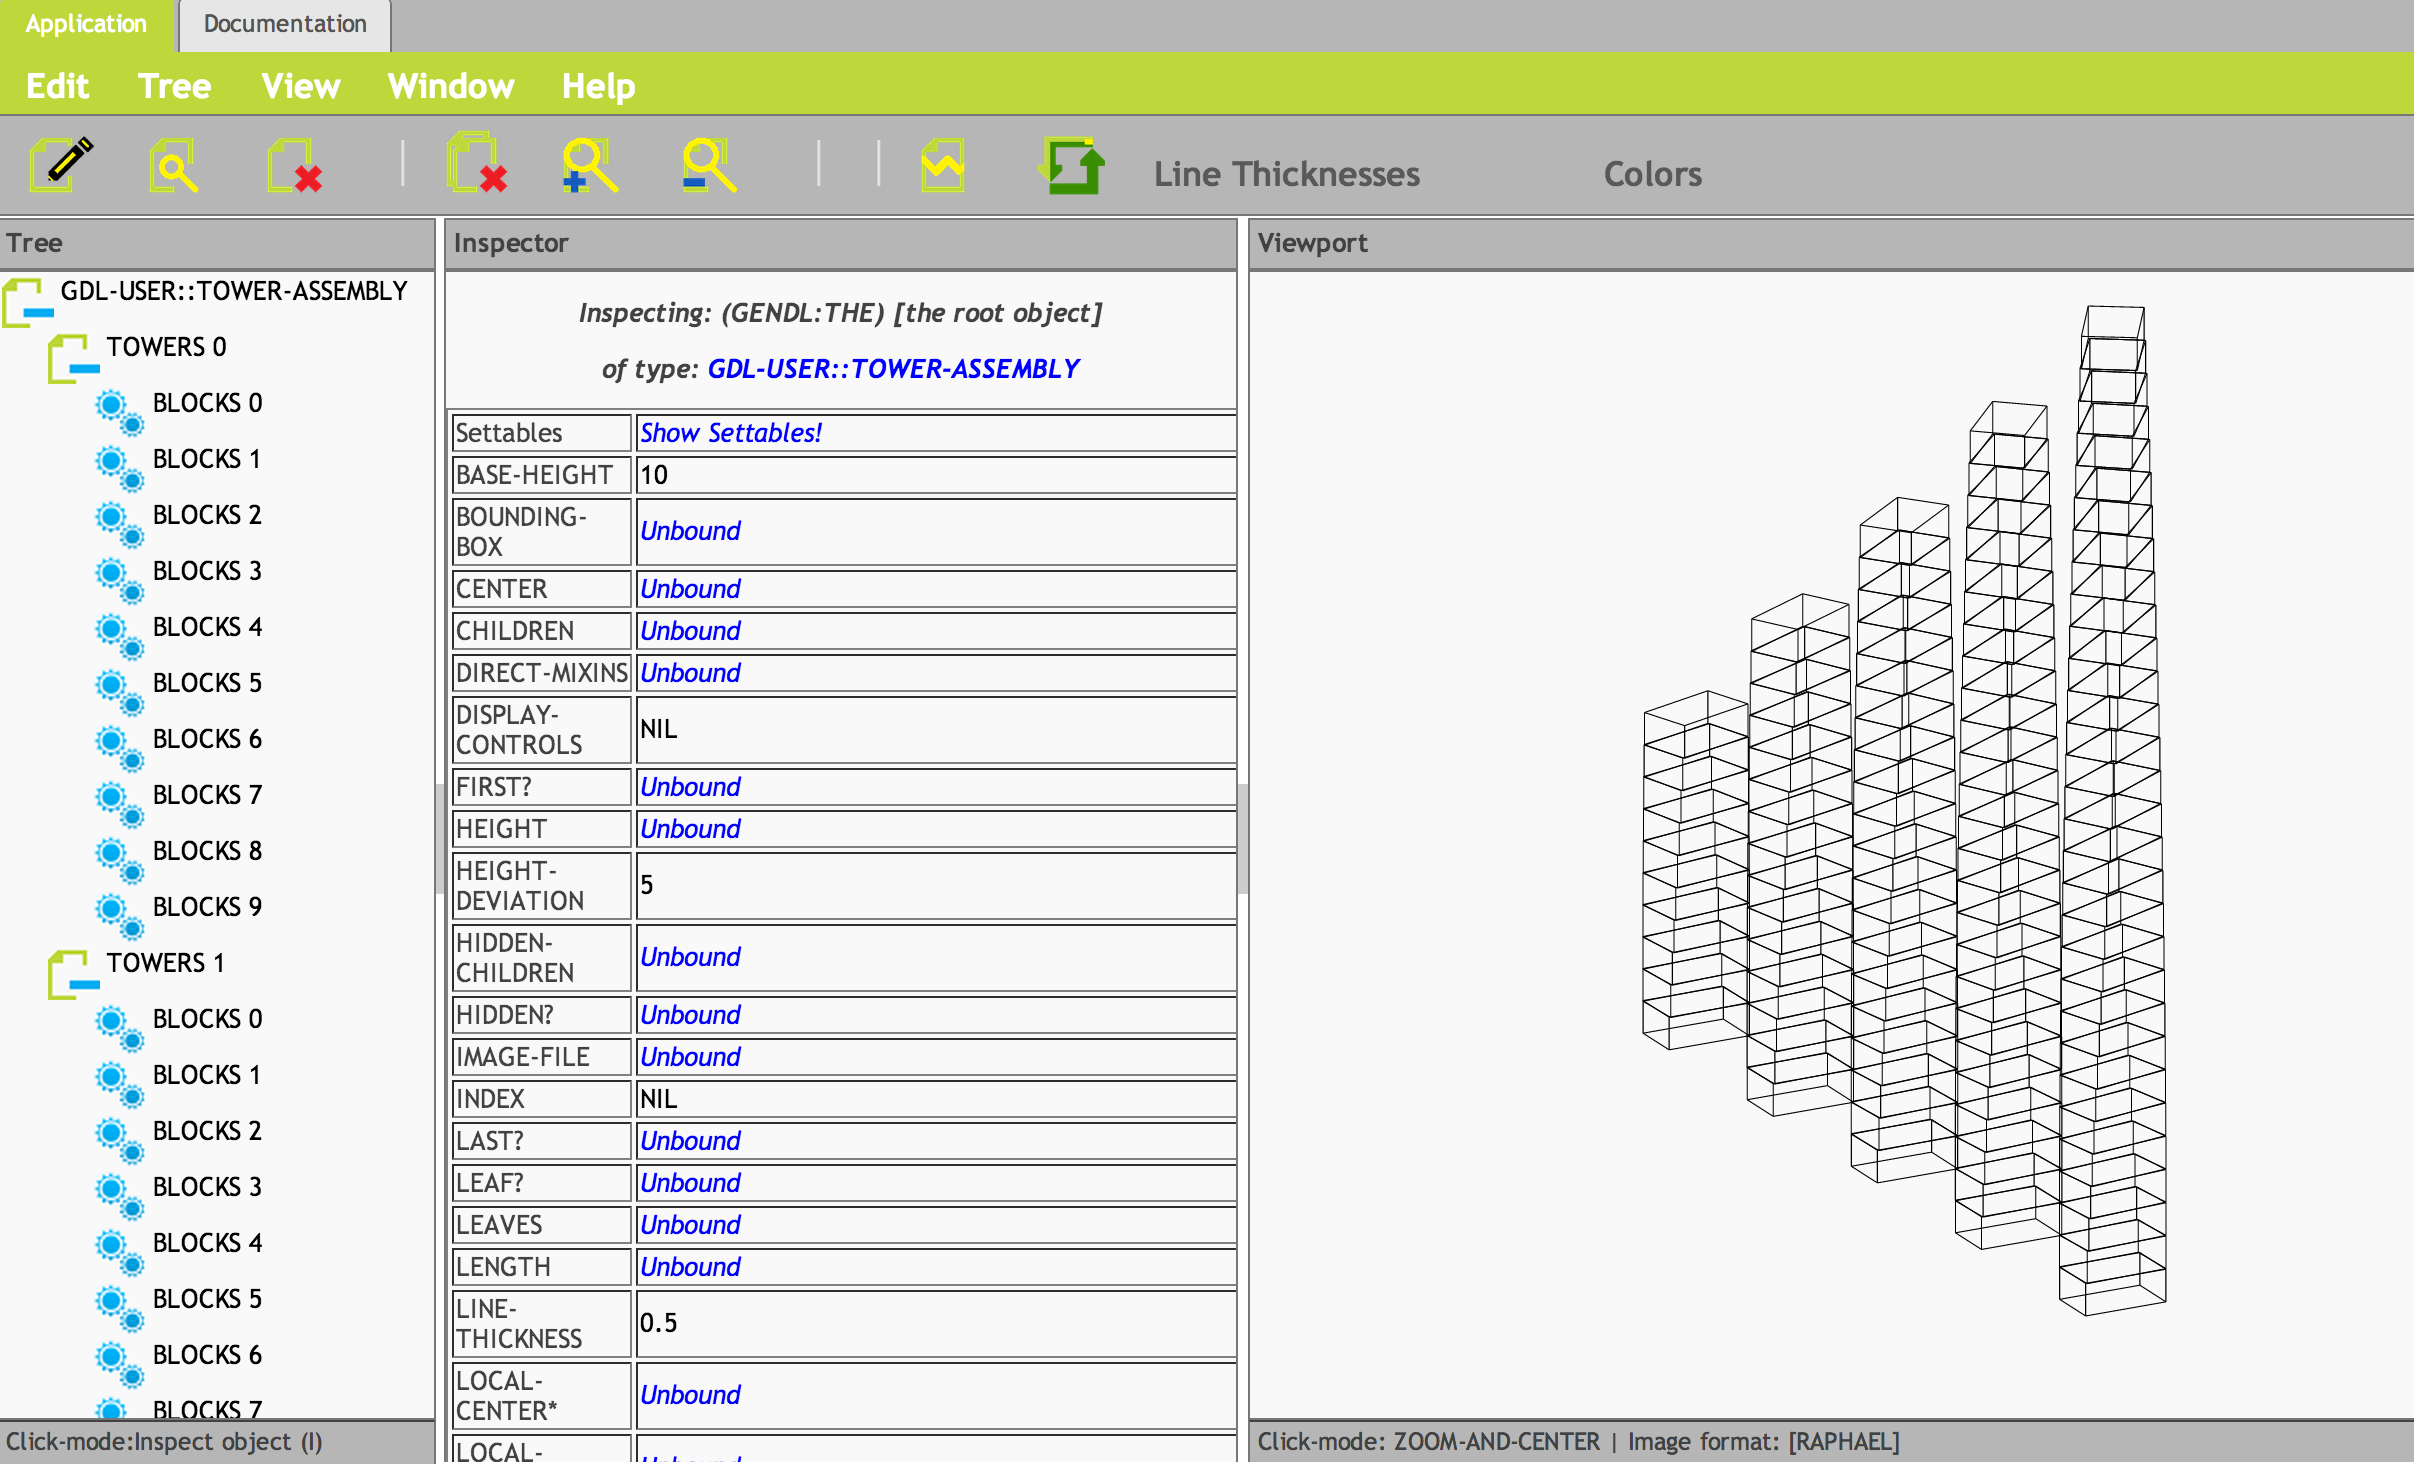
\includegraphics[width=4in,height=3in]{../images/tower-assembly-tasty.png}
\end{center}

\caption{Tower Assembly as displayed in Tasty}

\label{fig:tasty-assembly-tasty}

\end{figure}


\subsection{Mechanisms}

\label{subsec:mechanisms}


\begin{figure}
\begin{center}
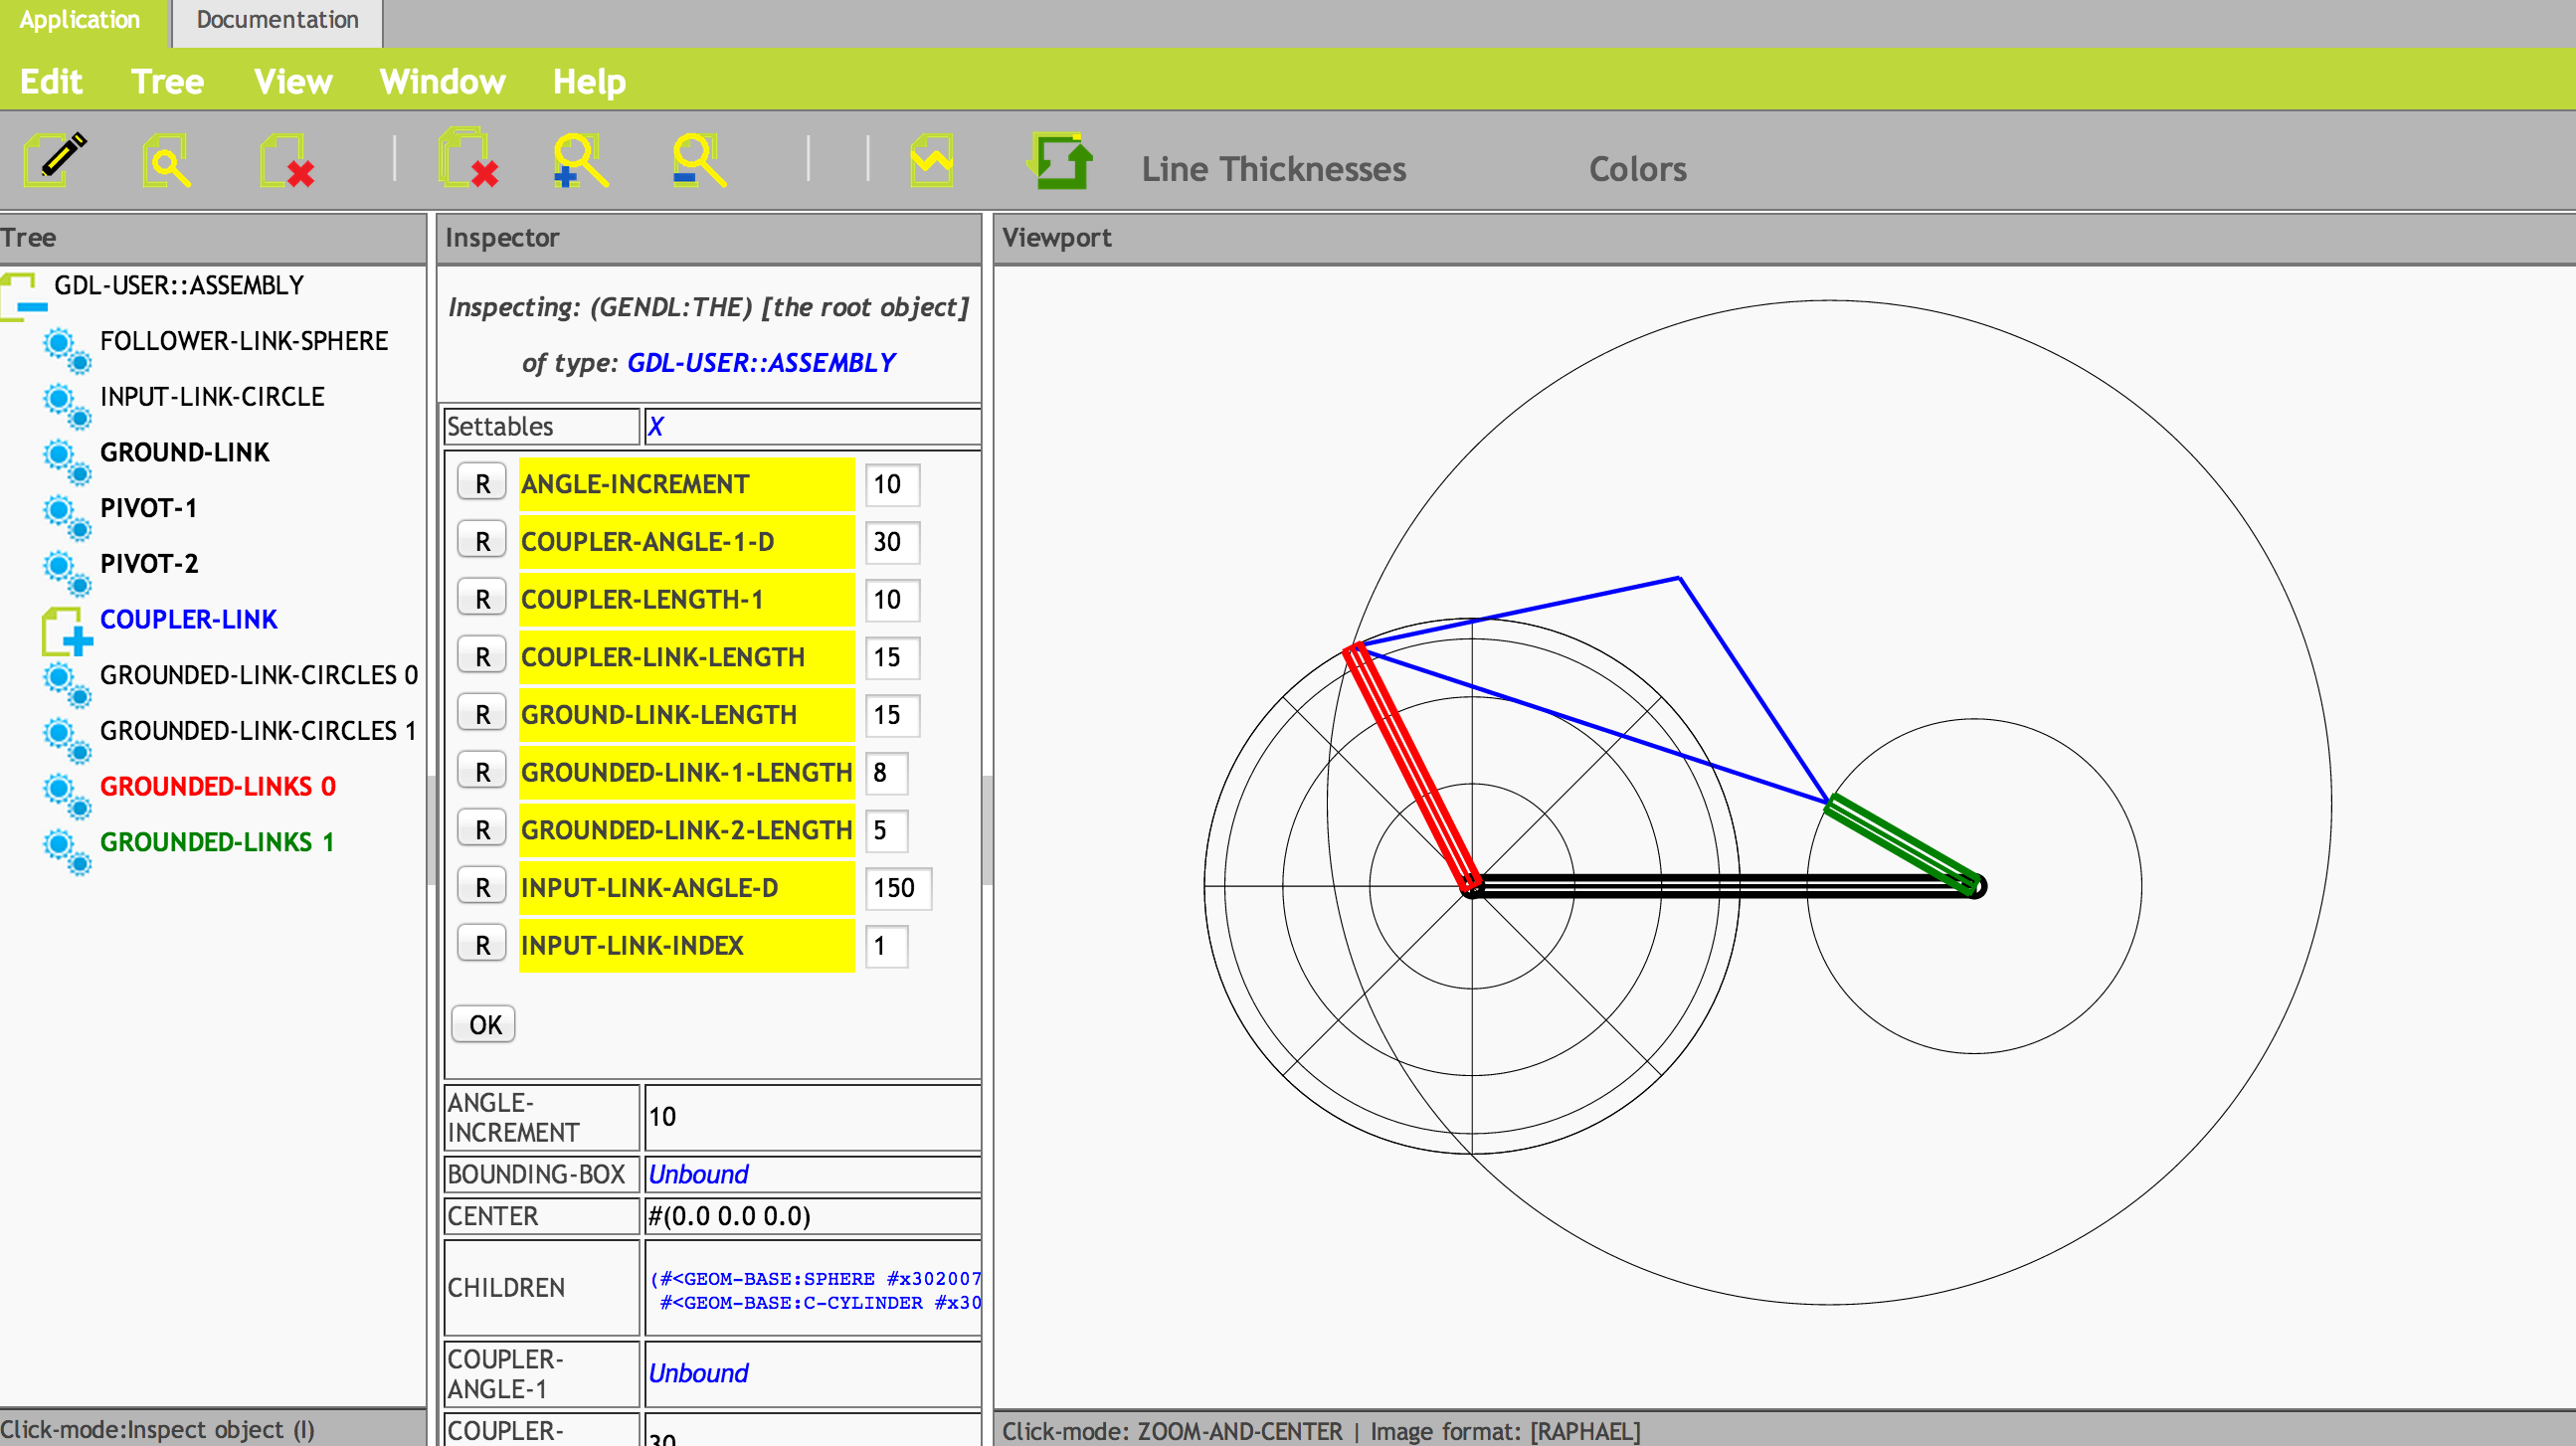
\includegraphics[width=5in,height=3in]{../images/4-bar-image.png}
\end{center}

\caption{Four-bar Link Mechanism}

\label{fig:4bar-image}

\end{figure}
GDL supports mechanisms without need for any special
features. By defining position and orientation of some objects to be
dependent on others, you can set up a mechanism. Figure 
\ref{fig:4bar-image} shows a standard four-bar link mechanism which is defined in the code in 
the file \href{run:../examples/4-bar-assembly.gdl}{4-bar-assembly.gdl} (this is in the examples directory\footnote{http://github.com/genworks/gendl/tree/master/documentation/tutorial/examples/} --- due to its length, the
     source is not printed in the manual.

\subsection{Other Geometric Primitives}

\label{subsec:othergeometricprimitives}

This chapter has focused primarily on the \texttt{box} primitive, because every type of geometric primitive is based upon a \emph{reference box}. Other primitives have their own sets of input-slots, and their
     own ways of being rendered in the various output formats. Basic
     2D primitives include:

\begin{itemize}

\item \texttt{circle} described on page 
\pageref{prim:circle}

\item \texttt{line} described on page 
\pageref{prim:line}

\item \texttt{arc} described on page 
\pageref{prim:arc}

\item \texttt{ellipse} described on page 
\pageref{prim:ellipse}

\item \texttt{bezier-curve}\footnote{The simple cubic bezier curve is supported
	       in the basic GDL and open-source Gendl. More
	       sophisticated NURBS-based curves and surfaces are
	       supported in the commercial GDL product when
	       accompanied with the SMLib geometry kernel. These are
	       covered in chapter 
\ref{chap:advanced-geometry}} described on page 
\pageref{prim:bezier-curve}

\end{itemize}

Basic 3D primitives include:

\begin{itemize}

\item \texttt{sphere} described on page 
\pageref{prim:sphere}

\item \texttt{cylinder} described on page 
\pageref{prim:cylinder}

\item \texttt{cone} described on page 
\pageref{prim:cone}

\item \texttt{global-polyline} described on page 
\pageref{prim:global-polyline}

\item \texttt{global-polygon-projection} described on page 
\pageref{prim:global-polygon-projection}

\item \texttt{global-filleted-polyline} described on page 
\pageref{prim:global-polyline}

\item \texttt{torus} described on page 
\pageref{prim:torus}

\item \texttt{route-pipe} described on page 
\pageref{prim:route-pipe}

\end{itemize}



\chapter{Custom User Interfaces in GDL}

\label{chap:customuserinterfacesingdl}



Another strength of GDL is the ability to create custom
web-based user interfaces. GDL contains a built-in web server and
supports the creation of generative \emph{web-based} user interfaces\footnote{GDL does not contain support for native desktop
GUI applications. Although the host Common Lisp
environment (e.g. Allegro CL or LispWorks) may contain a GUI builder
and Integrated Development Environment, and you are free to use these,
GDL does not provide specific support for them.}. Using the same \texttt{define-object} syntax which you have already encountered, you can define
web pages, sections of web pages, and form elements.
Your UI elements generate standard HTML, CSS, JavaScript, and can use
any external client-side libraries as with any standard web application.  AJAX support is
built-in, making it easy for server and UI elements to communicate asynchronously.



In order to create a web application in GDL, you should have a working
knowledge of the semantics of HTML, for which many explanations are available
online and in print.  For syntax, you can use an HTML-generation library such as \href{http://weitz.de/cl-who}{CL-WHO}\footnote{http://weitz.de/cl-who} or \href{http://www.franz.com/support/documentation/current/doc/aserve/htmlgen.html}{HTMLGen}\footnote{http://www.franz.com/support/documentation/current/doc/aserve/htmlgen.html}, both of which are built into GDL.  In this tutorial we will use CL-WHO, so in what folows,
we will assume that you are already familiar with its features as documented in \href{http://weitz.de/cl-who}{http://weitz.de/cl-who}.



\section{Package and Environment for Web Development}

\label{sec:packageandenvironmentforwebdevelopment}



The \texttt{:gwl} package\footnote{The acronym "GWL" stands
for Generative Web Language} contains a set of primitive objects and functions provided by
GDL for building web applications.



Similarly to \texttt{gdl:define-package}, you can use \texttt{gwl:define-package}
to create a working package which has access to the symbols you will need for building a
web application (in addition to the other GDL symbols).



The \texttt{:gwl-user} package is pre-defined and may be used for practice
work. For real projects, you should define your own package using \texttt{gwl:define-package}.



The YADD\footnote{YADD is accessible with \texttt{http://localhost:9000/yadd}.} reference documentation for package
GWL provides detailed specifications for all the primitive objects and functions.



\section{Web Page Objects}

\label{sec:webpageobjects}



To make a GDL object presentable as a web page, the following two
steps are needed:

\begin{enumerate}

\item Mix \texttt{base-ajax-sheet} into the object definition.

\item Within the object, define the GDL message \texttt{main-sheet-body} returning an HTML string.

\end{enumerate}





As soon the object is defined, the object's page becomes accessible at the URL

\begin{quote}
\texttt{http://localhost:9000/make?object=\emph{classname}}

\end{quote}
where \texttt{\emph{classname}} is the object name (including the package name).  Connecting to this
URL starts a new web server session and creates an instance of the object unique to that session\footnote{This is done by redirecting the response to a unique URL identified by a \emph{session ID}.
The session ID is constructed from a combination of the current date and time, along with a pseudo-random number.}.
This ensures that each user of your application site will see their own specific instance of the object.



The \texttt{main-sheet-body} message can be either a computed slot or a GDL function.  It should
produce a string of the HTML to be placed in the body of the page, i.e. between the \texttt{<body>} and
\texttt{</body>} tags.  The \texttt{<head>} of the page is filled in automatically by GDL, and can be
customized in various ways.



The easiest way to produce a valid \texttt{main-sheet-body} string is with the GWL convenience macro
\texttt{with-cl-who-string}.  This is a wrapper for the CL-WHO macro \texttt{with-html-output} which
additionally establishes the default environment for outputting an HTML string within a GWL application.



Figure 
\ref{fig:gwl-hello-world} is an example of a simple static web page.
\begin{figure}
\begin{lrbox}{\boxedverb}
\begin{minipage}{\linewidth}
{\small

\begin{verbatim}(in-package :gwl-user)

;; http://localhost:9000/make?object=gwl-user::hello-world
(define-object hello-world (base-ajax-sheet)
  :computed-slots
    ((main-sheet-body
       (with-cl-who-string ()
         (:p "Hello World!")))))

\end{verbatim}}
\end{minipage}
\end{lrbox}
\fbox{\usebox{\boxedverb}}

\caption{Simple Static Page}

\label{fig:gwl-hello-world}

\end{figure}




This simple framework can also be used to create dynamic content, as illustrated in figure 
\ref{fig:gwl-president-table}.
Note that CL-WHO symbols such as \texttt{htm}, \texttt{str}, and \texttt{fmt} are available in GWL without
package qualification. See \href{http://weitz.de/cl-who}{http://weitz.de/cl-who} for an explanation of
dynamic HTML generation in CL-WHO.
\begin{figure}
\begin{lrbox}{\boxedverb}
\begin{minipage}{\linewidth}
{\small

\begin{verbatim}(in-package :gwl-user)

(define-object president ()
  :input-slots
  (name term))

;; http://localhost:9000/make?object=gwl-user::presidents
(define-object presidents (base-ajax-sheet)
  :input-slots
  ((data (list (list :name "Carter" :term 1976)
               (list :name "Reagan" :term 1980)
               (list :name "Bush" :term 1988)
               (list :name "Clinton" :term 1992))))

  :objects
  ((presidents :type 'president
               :sequence (:size (length (the data)))
               :name (getf (nth (the-child index) (the data)) :name)
               :term (getf (nth (the-child index) (the data)) :term)))

  :computed-slots
  ((main-sheet-body
    (with-cl-who-string (:indent t)
      (htm
       (:p (:c (:h3 (fmt "Info on ~a Presidents:"
                         (length (list-elements (the presidents)))))))
       ((:table :border 1)
        (:tr (:th "Name") (:th "Term"))
        (dolist (president (list-elements (the presidents)))
          (htm      
           (:tr (:td (str (the-object president name)))
                (:td (str (the-object president term))))))))))))

\end{verbatim}}
\end{minipage}
\end{lrbox}
\fbox{\usebox{\boxedverb}}

\caption{Dynamic Content Using CL-WHO}

\label{fig:gwl-president-table}

\end{figure}




\section{Page URLs}

\label{sec:pageurls}



Objects based on \texttt{base-ajax-sheet} are automatically available from the server at the
URL of the form \texttt{http://localhost:9000/make?object=\emph{classname}}.  This is useful during
debugging, but for real projects, you should define a more direct URL.  You do that using the
CL function \texttt{(gwl:publish-gwl-app \emph{path} \emph{classname})}.  For example,

\begin{quote}
\texttt{(gwl:publish-gwl-app "/greeting" "gwl-user::hello-world")}

\end{quote}
will make the \texttt{gwl-user::hello-world} object accessible at the URL \texttt{http://localhost:9000/greeting}.



\section{Page Customizations}

\label{sec:pagecustomizations}



In addition to specifying the body html via \texttt{main-sheet-body}, you can
customize the page by optionally adding certain messages to your object:

\begin{itemize}

\item Message \texttt{title} can be used to specify the title of the web page

\item Message \texttt{doctype-string} is the string to place at the very start
of the document (it defaults to \texttt{"<!DOCTYPE HTML>"})

\item Message \texttt{additional-header-content} can contain any additional
HTML you want to go into the page's \texttt{<head>} section.

\item Message \texttt{body-class} can specify the CSS \texttt{class} attribute for the \texttt{<body>} tag.

\item Message \texttt{body-onload} can be a string of Javascript to go
into the \texttt{onload} event attribute of the \texttt{<body>} tag.

\item Message \texttt{body-onpageshow} can be a string of Javascript to go
into the \texttt{onpageshow} event attribute of the \texttt{<body>} tag.

\end{itemize}





We will be using some of these customizations in the examples below.



\section{Debugging}

\label{sec:debugging}



\texttt{base-ajax-sheet} provides the \texttt{development-links} message with
links for functionality useful during development, currently consisting of a Refresh! link and a Break
link.  It is typically used as follows:

\begin{verbatim}(main-sheet-body
  (with-cl-who-string ()
    (when *developing?* (str (the development-links)))
    ;; Rest of page definition goes here
    ...))
\end{verbatim}



\section{Page Links}

\label{sec:pagelinks}



In order to allow HTML links between page objects, GDL implements a scheme that assigns
URL's to individual page instances.  In order to do this efficiently, GDL maintains a table of
root-level instances, and identifies page instances relative to their root instance.  For this reason,
and in order for dependency-tracking to work properly, all pages in a GDL application must belong to
the same tree, i.e. they must share a common root page object.



You can generate a hyperlink (an \texttt{<A>} tag) to a particular \texttt{base-ajax-sheet} page
by invoking the \texttt{write-self-link} GDL function on the page instance. \texttt{write-self-link} accepts
a number of keyword arguments to customize the link:

\begin{itemize}

\item You specify the text to be displayed as the link with the \texttt{:display-string} argument

\item You can direct the link to a specific anchor within the page with the \texttt{:local-anchor} argument

\item You can specify various tag attributes of the \texttt{<A>} tag:

\begin{itemize}

\item Argument \texttt{:target} for the \texttt{target} attribute

\item Argument \texttt{:on-mouse-over} for the \texttt{onmouseover} attribute

\item Argument \texttt{:on-mouse-out} for the \texttt{onmouseout} attribute

\item Argument \texttt{:on-click} for the \texttt{onclick} attribute

\item Argument \texttt{:title} for the \texttt{title} attribute

\item Argument \texttt{:class} for the \texttt{class} attribute

\item Argument \texttt{:id} for the \texttt{id} attribute

\end{itemize}



\end{itemize}





In order to help create hierarchical multi-page sites, \texttt{base-ajax-sheet} also provides
a \texttt{write-back-link} GDL function for the purpose of generating a link back to the parent page object.
It accepts all the same arguments as \texttt{write-self-link}.



Figure 
\ref{fig:gwl-president-links} shows a modification of 
\ref{fig:gwl-president-table}
where we put detailed information about each president on a separate page, and provide links to these individual
pages from a summary page.  Each child page contains a link to return back to the summary.
\begin{figure}
\begin{lrbox}{\boxedverb}
\begin{minipage}{\linewidth}
{\small

\begin{verbatim}(in-package :gwl-user)

(define-object president-page (base-ajax-sheet)
  :input-slots
  (name term)

  :computed-slots
  ((title
    (format nil "Term for President ~a:" (the name)))
   (main-sheet-body
    (with-cl-who-string (:indent t)
      (the (write-back-link :display-string "&lt;Back"))
      (:p (:c (:h3 (the title))))
      (:p (str (the term)))))))


;; http://localhost:9000/make?object=gwl-user::presidents-with-links
(define-object presidents-with-links (base-ajax-sheet)
  :input-slots
  ((data (list (list :name "Carter" :term 1976)
               (list :name "Reagan" :term 1980)
               (list :name "Bush" :term 1988)
               (list :name "Clinton" :term 1992)))
   (table-border 1))

  :objects
  ((presidents :type 'president-page
               :sequence (:size (length (the data)))
               :name (getf (nth (the-child index) (the data)) :name)
               :term (getf (nth (the-child index) (the data)) :term)))

  :computed-slots
  ((title (format nil "Links to ~a Presidents:"
                  (length (list-elements (the presidents)))))
   (main-sheet-body
    (with-cl-who-string (:indent t)
      (htm
       (:p (:c (:h3 (the title))))
       ((:table :border (the table-border))
        (:tr (:th "Name"))
        (dolist (president (list-elements (the presidents)))
          (htm      
           (:tr (:td (the-object
                      president
                      (write-self-link :display-string
                                       (the-object president name)))))))))))))


\end{verbatim}}
\end{minipage}
\end{lrbox}
\fbox{\usebox{\boxedverb}}

\caption{Hyperlinking}

\label{fig:gwl-president-links}

\end{figure}




\section{Input Using Forms}

\label{sec:inputusingforms}



GWL provides a macro \texttt{with-html-form} to obtain input from the user
with an HTML form.  In the body of the form, you specify input fields using standard HTML
form controls.  When the user submits the form, GDL processes the form input values in two
ways:

\begin{itemize}

\item When the name of an form field matches the name of a \texttt{:settable} computed-slot in the object, GDL will automatically infer its type, do
appropriate conversions, and set the slot the its new value\footnote{If the type of a slot
can vary, it is best to make its default be a string and parse the string yourself e.g. with
the \texttt{read-safe-string} function.}.

\item Any input values that do not match a suitable slot are available 
from the \texttt{query-plist} message, which returns a plist mapping
keywords representing form field names to the corresponding input value strings

\end{itemize}





Figure 
\ref{fig:gwl-hello-world-form} shows how we can extend the simple
Hello World application of 
\ref{fig:gwl-hello-world} to allow the user to
customize both the name and the greeting.
\begin{figure}
\begin{lrbox}{\boxedverb}
\begin{minipage}{\linewidth}
{\small

\begin{verbatim}(in-package :gwl-user)

;; http://localhost:9000/make?object=gwl-user::hello-world-form
(define-object hello-world-form (base-ajax-sheet)
  :input-slots
  ((greetings '("Hello"
                "Hola"
                "Bonjour"
                "Habari"
                "Namaste"
                "Aloha"
                "Ciao")))
  
  :computed-slots
  ((username "World" :settable)
   (greeting (first (the greetings)) :settable)
   
   (title (format nil "Greeting for ~a" (the username)))
   (main-sheet-body
    (with-cl-who-string ()
      (:p (fmt "~a ~a!" (the greeting) (the username)))
      (:hr)
      (with-html-form (:cl-who? t)
        (:p
         (:label :for 'greeting "Select greeting: ")
         ((:select :name 'greeting)
          (dolist (val (the greetings))
            (with-cl-who ()
              ((:option :value val
                        :selected (and (equalp val (the greeting)) "selected"))
               (esc val))))))
        (:p
         (:label :for 'username "Enter new name: ")
         (:input :type :text :name 'username :value (the username)))
        (:p (:button :type :submit "UPDATE")))))))

\end{verbatim}}
\end{minipage}
\end{lrbox}
\fbox{\usebox{\boxedverb}}

\caption{Input Using Forms}

\label{fig:gwl-hello-world-form}

\end{figure}




\subsection{Form Controls}

\label{subsec:formcontrols}



GDL provides a set of primitives useful for generating the
standard HTML form controls in the body of \texttt{with-html-form}.
These should be instantiated as child objects in the page.  They provide a
\texttt{html-string} message which returns the HTML for the control.



The form controls provided by GDL are documented in YADD\footnote{YADD
is accessible with \texttt{http://localhost:9000/yadd}.} and in the reference appendix
of this manual. Examples of available form controls are:

\begin{itemize}

\item \texttt{text-form-control}

\item \texttt{checkbox-form-control}

\item \texttt{menu-form-control}

\item \texttt{radio-form-control}

\item \texttt{text-form-control}

\item \texttt{button-form-control}

\end{itemize}





These form controls are customizable by mixing them into
	   your own specific form controls (although this often is not
	   necessary). New form controls such as for numbers, dates,
	   etc will soon be added to correspond to latest HTML
	   standards.



Figure 
\ref{fig:gwl-hello-world-controls} reimplements the Hello World form from the last section
using form controls.  The functionality is the same but the source is shorter and simpler to read and understand.
\begin{figure}
\begin{lrbox}{\boxedverb}
\begin{minipage}{\linewidth}
{\small

\begin{verbatim}(in-package :gwl-user)

;; http://localhost:9000/make?object=gwl-user::hello-world-controls
(define-object hello-world-controls (base-ajax-sheet)
  :input-slots
  ((greetings '("Hello"
                "Hola"
                "Bonjour"
                "Habari"
                "Namaste"
                "Aloha"
                "Ciao")))

  :objects
  ((username-control :type 'text-form-control
                     :prompt "Enter new name: "
                     :default "World")
   (greeting-control :type 'menu-form-control
                     :prompt "Select Greeting: "
                     :size 1 :choice-list (the greetings)
                     :default (first (the greetings))))

  :computed-slots
  ((title (format nil "Greeting for ~a" (the username-control value)))
   (main-sheet-body
    (with-cl-who-string ()
      (:p (fmt "~a ~a!" (the greeting-control value) (the username-control value)))
      (:hr)
      (with-html-form (:cl-who? t)
        (:p (str (the greeting-control html-string)))
        (:p (str (the username-control html-string)))
        (:p (:button :type :submit "UPDATE")))))))

\end{verbatim}}
\end{minipage}
\end{lrbox}
\fbox{\usebox{\boxedverb}}

\caption{Using Form Controls}

\label{fig:gwl-hello-world-controls}

\end{figure}




\section{Interactive Applications using AJAX}

\label{sec:interactiveapplicationsusingajax}



Input using traditional HTML forms requires the user to explicitly "submit" each update
request, and then the application responds by reloading the whole page.  The \href{http://en.wikipedia.org/wiki/Ajax\_(programming)}{AJAX}\footnote{http://en.wikipedia.org/wiki/Ajax\_(programming)} methodology allows web
applications to autonomously contact the server, and to change page content dynamically in
response, leading to a more interactive user experience.



GDL has built-in support for AJAX, using its usual convenient generative approach.
You use child objects to model independently updatable sections of the web pgae, and the dependency
tracking engine which is built into GDL automatically manages of which sections of the
page need to be updated after a request.



Moreover, the state of the internal GDL model which
represents the page and the page sections is kept identical to the
displayed state of the page. This means that if the user hits the
``Refresh'' button in the browser, the state of the page will remain
unchanged. This ability is not available in some other AJAX
frameworks.



\subsection{AJAX Event Handling}

\label{subsec:ajaxeventhandling}



An AJAX application works by contacting the server
in response to \href{https://en.wikipedia.org/wiki/DOM\_events}{HTML events}\footnote{https://en.wikipedia.org/wiki/DOM\_events} such as "onclick"
or "onfocus".  GDL provides the function \texttt{gdl-ajax-call} to generate
the JavaScript to handle such events by invoking GDL functionality on the server.



For example, the following snippet

\begin{verbatim}((:span :onclick (the (gdl-ajax-call :function-key :restore-defaults!)))
        "Press Me")
\end{verbatim}will produce a piece of text ''Press Me'' which, when pressed, will call \texttt{restore-defaults!}
in the page's object on the server. If \texttt{restore-defaults!} is not defined, an error will result.



\texttt{gdl-ajax-call} can also update form control values on the server by using the \texttt{:form-controls} keyword argument. For details, see the \texttt{gdl-ajax-call} documentation in
YADD\footnote{YADD is accessible with \texttt{http://localhost:9000/yadd}.} and the reference appendix.



For convenience, GDL form-controls provide direct support for AJAX with the \texttt{:ajax-submit-on-change?}
argument, which is equivalent to invoking \texttt{gdl-ajax-call} for the control's "onchange" event.



\subsection{AJAX Page Updating}

\label{subsec:ajaxpageupdating}



In order to have the capacity to change itself in response to AJAX calls, a page must be structured
as one or more \texttt{sheet-section} child objects.  Sheet sections provide a \texttt{main-div} message
which computes the HTML for the section and registers the section as subject to AJAX update handling.  The
main page should include the \texttt{main-div} of each child sheet section in its \texttt{main-sheet-body}.



The sheet section definition should specify the section's HTML in the \texttt{inner-html} input slot.
This plays the same role as the \texttt{main-sheet-body} does in the page.



Figure 
\ref{fig:gwl-hello-world-ajax} reimplements the Hello World form from the last section
using AJAX.  Note that we don't need the explicit UPDATE button any more, as the changes the user makes take effect
immediately due to the use of \texttt{:ajax-submit-on-change?} argument in each of the form controls.
\begin{figure}
\begin{lrbox}{\boxedverb}
\begin{minipage}{\linewidth}
{\small

\begin{verbatim}(in-package :gwl-user)

;; http://localhost:9000/make?object=gwl-user::hello-world-ajax
(define-object hello-world-ajax (base-ajax-sheet)
  :input-slots
  ((greetings '("Hello"
                "Hola"
                "Bonjour"
                "Habari"
                "Namaste"
                "Aloha"
                "Ciao")))

  :objects
  ((username-control :type 'text-form-control
                     :prompt "Enter new name: "
                     :default "World"
                     :ajax-submit-on-change? t)
   (greeting-control :type 'menu-form-control
                     :prompt "Select Greeting: "
                     :size 1 :choice-list (the greetings)
                     :default (first (the greetings))
                     :ajax-submit-on-change? t)

   (main-section
    :type 'sheet-section
    :inner-html (with-cl-who-string ()
                  (:p (fmt "~a ~a!" (the greeting-control value) (the username-control value)))
                  (:hr)
                  (with-html-form (:cl-who? t)
                    (:p (str (the greeting-control html-string)))
                    (:p (str (the username-control html-string)))))))

  :computed-slots
  ((title (format nil "Greeting for ~a" (the username-control value)))
   (main-sheet-body
    (with-cl-who-string ()
      (str (the main-section main-div))))))

\end{verbatim}}
\end{minipage}
\end{lrbox}
\fbox{\usebox{\boxedverb}}

\caption{AJAX}

\label{fig:gwl-hello-world-ajax}

\end{figure}




\subsection{Including Graphics}

\label{subsec:includinggraphics}



The fundamental mixin or child type to make a graphics viewport is \texttt{base-ajax-graphics-sheet}. This object definition takes several optional input-slots, but the most essential are the \texttt{:display-list-objects} and the \texttt{:display-list-object-roots}. As indicated by their names, you specify a list of nodes to include in
the graphics output with the \texttt{:display-list-objects}, and a list of nodes whose \texttt{leaves} you want to display in the graphics output with the \texttt{:display-list-object-roots}. View controls, rendering format, action to take when clicking on objects, etc, 
can be controlled with other optional input-slots.


\begin{figure}
\begin{lrbox}{\boxedverb}
\begin{minipage}{\linewidth}
{\small

\begin{verbatim}(in-package :gwl-user)

(define-object box-with-inputs (base-ajax-sheet)
  
  :computed-slots
  ((use-raphael? t)
   (use-x3dom? t)
   
   (main-sheet-body 
    (with-cl-who-string ()
      (:p (when *developing?* (str (the development-links))))
      (:p (str (the inputs-section main-div)))
      (:table
       (:tr
        (dolist (viewport (list-elements (the viewport-sections)))
          (htm (:td (:td (str (the-object viewport main-div)))))))))))
  
  :objects
  ((box :type 'box
        :height (the inputs-section box-height value)
        :width (the inputs-section box-width value)
        :length (the inputs-section box-length value))
   
   (inputs-section :type 'inputs-section)

   (viewport-sections
    :type 'base-ajax-graphics-sheet
    :sequence (:size 2)
    :view-direction-default (ecase (the-child index)
                              (0 :top) (1 :trimetric))
    :image-format-default :raphael
    :display-list-objects (list (the box))
    :length 250 :width 250)))
  

 
(define-object inputs-section (sheet-section)
  
  :computed-slots
  ((inner-html (with-cl-who-string ()
                (:p (str (the box-length html-string)))
                (:p (str (the box-width html-string)))
                (:p (str (the box-height html-string))))))

  :objects 
  ((box-length :type 'text-form-control
               :default 25
               :ajax-submit-on-change? t)
   (box-width :type 'text-form-control
              :default 35
              :ajax-submit-on-change? t)
   (box-height :type 'text-form-control
               :default 45
               :ajax-submit-on-change? t)))


(publish-gwl-app "/box-with-inputs" 
                 "gwl-user::box-with-inputs")

;;
;; Access the above example with 
;; http://localhost:9000/make?object=gwl-user::box-with-inputs
;;

\end{verbatim}}
\end{minipage}
\end{lrbox}
\fbox{\usebox{\boxedverb}}

\caption{Including Graphics in a Web Page}

\label{fig:gwl-5}

\end{figure}

\begin{figure}
\begin{center}
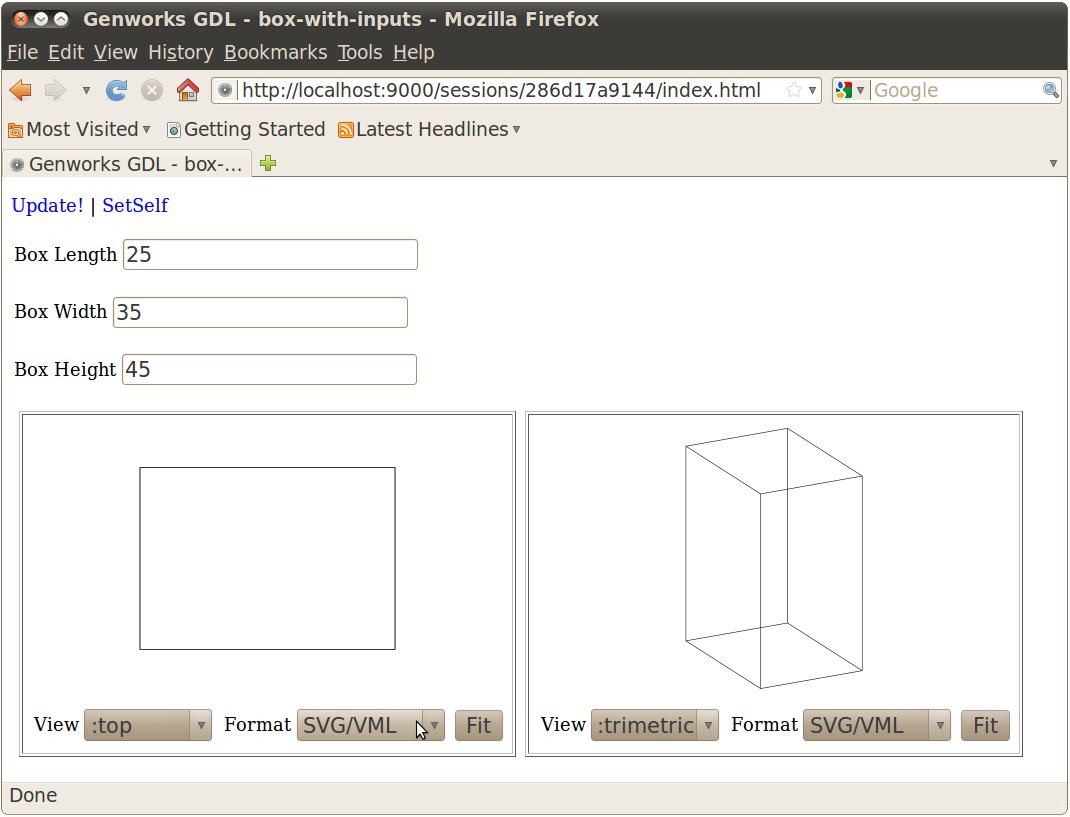
\includegraphics[width=5in,height=4in]{../images/gwl-5.png}
\end{center}

\caption{Including Graphics}

\label{fig:gwl-5-image}

\end{figure}


The example in Figure 
\ref{fig:gwl-5} contains a simple box with two graphics viewports
and ability to modify the length, height, and and width of the box:



This will produce a web browser output similar to what is shown in Figure 
\ref{fig:gwl-5-image}.



Note the following from this example:

\begin{itemize}

\item The \texttt{(:use-raphael? t)} enables raphael for SVG or VML output.

\item The \texttt{:raphael} image-format generates SVG or VML, depending on the browser.

\item We conditionally include development-links for full Update and SetSelf! actions.

\item We include two viewports in the \texttt{main-sheet-body}, elements from a sequence of size 2.

\item In the inputs-section, we use
                  the \texttt{html-string} message from each
                  form-control to display the default
                  decoration (prompt, etc).

\end{itemize}





\chapter{More Common Lisp for GDL}

\label{chap:morecommonlispforgdl}



\chapter{Advanced GDL}

\label{chap:advancedgdl}



\chapter*{Upgrade Notes}

\label{chap:upgradenotes}

GDL 1580 marked the end of a major branch of GDL development,
and 1581 was an upgraded new version, which in turn has now been
supplanted by 1582.

This addendum lists the typical modifications you will want to
consider for upgrading from GDL 1580 to GDL 1582, or later versions.

\begin{itemize}

\item (make-gdl-app ..) is now available for 1582. We have
made available an Enterprise Edition of 1582 which includes the
make-gdl-app function, which creates Runtime applications without the
compiler or GDL development facilities.  If you are an Enterprise
licensee, and are ready to release Runtime applications on 1582, and
you have not received information on the Enterprise Edition, please
contact support@genworks.com

\item (register-asdf-systems) and the \texttt{"3rdpty/"} directory are no longer needed or available. Instead, we depend on the Quicklisp
system. Details of Quicklisp are available at \texttt{http://www.quicklisp.org}. See Section 
\ref{subsec:compilingandloadingasystem} for information about how to use Quicklisp with GDL.

\item There is a system-wide \texttt{gdlinit.cl} in the application directory, and depending on the
       particular release you have, this may have some default
       information which ships with GDL. There is a personal \texttt{gdlinit.cl} in home directory, which you should modify if you want to
       customize anything.

\item Slime debugging is different from the ELI emacs debugger. The main thing to know is 
to press ``a'' or ``q'' to pop out of the current error. Full documentation for the Slime debug mode
is available with the \href{http://common-lisp.net/project/slime/doc/html/Debugger.html}{Slime documentation}.

\item color-themes -- GDL now ships with the Emacs
       color-theme package. You can select a different color theme with \texttt{M-x color-theme-select}. Press [Enter] or middle-mouse on a color theme to apply it.

\item GDL files can now end with \texttt{.lisp} or \texttt{.gdl}. The new \texttt{.gdl} extension will work for emacs Lisp mode and will work with
	 cl-lite, ASDF, and Quicklisp for including source files in application systems. We recommend migrating
to the new \texttt{.gdl} extension for files containing \texttt{define-object}, \texttt{define-format}, and \texttt{define-lens} forms, and any other future toplevel defining forms introduced by GDL, in order to distinguish 
from files containing raw Common Lisp code.

\item in gdlAjax, HTML for a sheet-section is given in the slot called \texttt{inner-html} instead of \texttt{main-view}. This name change was made to clarify what exactly is
	 expected in this slot -- it is the innerHTML of the page
	 division represented by the current sheet-section. If you
	 want to make your code back-compatible with GDL 1580, you can
	 use the following form in place of old occurences of \texttt{main-view}: 

\begin{verbatim}... #+allegro-v8.1 main-view #-allegro-v8.1 inner-html ...
\end{verbatim}

\item (update-gdl ..) is not yet available for 1582. Instead
of updating incrementally with patches, the intention starting with
GDL 1582 is for full GDL releases to be made available approximately
monthly. Less frequent Long Term Maintenance (``LTS'') releases will
also be made available along with a new simpler maintenance patch
system.

\end{itemize}



\chapter{Reference for GDL Objects and Operators}

\label{chap:referenceforgdlobjectsandoperators}



\section{CL-LITE (Compile-and-Load Lite Utility)}

\label{sec:cl-lite(compile-and-loadliteutility)}





\subsection{Object Definitions}

\label{subsec:objectdefinitions}



\begin{itemize}

\item \index{CODEBASE-DIRECTORY-NODE}
\label{prim:codebase-directory-node}
\textbf{CODEBASE-DIRECTORY-NODE}


\textbf{
\underline{Mixins:}} DIRECTORY-NODE





\begin{description}

\item [
\underline{Description}]


Models a filesystem directory for use by the cl-lite program.



\end{description}








\textbf{
\underline{Input slots (optional):}}

\begin{description}

\item [Bin-subdir-names]
\index{Bin-subdir-names
[codebase-directory-node]}\emph{List of strings}

 Identifies the names of directories considered to hold binaries.
Default is (list "bin" "patch")




\item [Create-fasl?]
\index{Create-fasl?
[codebase-directory-node]}\emph{Boolean}

 Determines whether to write a concatenated fasl for the build. Defaults to nil.
NOTE: this is not currently supported in cl-lite.




\item [Fasl-output-name]
\index{Fasl-output-name
[codebase-directory-node]}\emph{String}

 Names the built concatenated fasl when \texttt{(the create-fasl?)} is non-nil.
Defaults to \texttt{(the local-name)}




\item [Fasl-output-path]
\index{Fasl-output-path
[codebase-directory-node]}\emph{String or pathname object}

 Designates the pathname for the filesystem directory in which
the built concatenated fasls are written. Defaults to \texttt{(glisp:temporary-folder)}




\item [Fasl-output-type]
\index{Fasl-output-type
[codebase-directory-node]}\emph{String}

 Names the fasl extension used by the compiler. Defaults to the local fasl output type.




\item [Load-always?]
\index{Load-always?
[codebase-directory-node]}\emph{Boolean}

 Determines whether to load the individual compiled fasls even if the source has not changed.
Defaults to nil (i.e. we assume we are loading into a clean system and need all the initial definitions.).




\item [Source-files-to-ignore]
\index{Source-files-to-ignore
[codebase-directory-node]}\emph{List of strings}

 Lists directory names which should be ignored as having
compilable source code for the build.




\item [Special-subdir-names]
\index{Special-subdir-names
[codebase-directory-node]}\emph{List of strings}

 Identifies the names of directories which are part of a vc-system control files
and therefore should be treated as special subdirectories.
Default is (list "CVS")




\item [Type-mapping]
\index{Type-mapping
[codebase-directory-node]}\emph{Plist of keywords and lists of strings}

 Maps directory names to their default type classifications.




\end{description}






\textbf{
\underline{Computed slots:}}

\begin{description}

\item [Strings-for-display]
\index{Strings-for-display
[codebase-directory-node]}\emph{String or List of Strings}

 Determines how the name of objects of
this type will be printed in most places.  This defaults to the
name-for-display (generally the part's name as specified in its
parent), followed by an index number if the part is an element of a
sequence.




\end{description}







\end{itemize}



\subsection{Function and Macro Definitions}

\label{subsec:functionandmacrodefinitions}



\begin{itemize}

\item \index{CL-PATCH}
\label{prim:cl-patch}
\textbf{CL-PATCH}

(TYPE NIL INTRO 
Traverses pathname in a manner identical to cl-lite, but only those
files for which the source is newer than the corresponding fasl
binary file (or for which the corresponding fasl binary file does
not exist) will be loaded. Use this for incremental updates where
the unmodified source files do not depend on the modified source
files.
)



\end{itemize}





\section{COM.GENWORKS.DOM }

\label{sec:com.genworks.dom}







\section{COM.GENWORKS.DOM-HTML }

\label{sec:com.genworks.dom-html}







\section{COM.GENWORKS.DOM-LATEX }

\label{sec:com.genworks.dom-latex}







\section{COM.GENWORKS.DOM-WRITERS }

\label{sec:com.genworks.dom-writers}







\section{COM.YOYODYNE.BOOSTER-ROCKET }

\label{sec:com.yoyodyne.booster-rocket}







\section{ENTERPRISE }

\label{sec:enterprise}







\section{GENDL (Base Core Kernel Engine) Nicknames: Gdl, Genworks, Base}

\label{sec:gendl(basecorekernelengine)nicknames:gdl,genworks,base}





\subsection{Object Definitions}

\label{subsec:objectdefinitions}



\begin{itemize}

\item \index{BASE-RULE-OBJECT}
\label{prim:base-rule-object}
\textbf{BASE-RULE-OBJECT}


\textbf{
\underline{Mixins:}} VANILLA-MIXIN





\begin{description}

\item [
\underline{Description}]


Encapsulates a basic computation, usually to be displayed to the user.
Typically this would be used as a mixin into a more sophisticated rule-object, but the type can be
 used to detect objects which should be processed as "rules."



\end{description}








\textbf{
\underline{Input slots (optional):}}

\begin{description}

\item [Rule-description]
\index{Rule-description
[base-rule-object]}\emph{String}

 Short description of the rule (generally one line). Defaults to NIL.




\item [Rule-description-help]
\index{Rule-description-help
[base-rule-object]}\emph{String}

 Verbose description of the purpose of the rule.




\item [Rule-result]
\index{Rule-result
[base-rule-object]}\emph{String}

 The basic return-value, or result, of evaluating the rule.




\item [Rule-result-help]
\index{Rule-result-help
[base-rule-object]}\emph{String}

 Verbose description of how the rule result is computed.




\item [Rule-title]
\index{Rule-title
[base-rule-object]}\emph{String}

 Title to be used with the rule object. Defaults to NIL.




\item [Strings-for-display]
\index{Strings-for-display
[base-rule-object]}\emph{String}

 Determines the rule's default name in various internal GDL contexts. Defaults to
the \texttt{rule-title}, or "Unnamed Rule" if \texttt{rule-title} is NIL.




\item [Suppress-display?]
\index{Suppress-display?
[base-rule-object]}\emph{Boolean}

 Determines whether the rule is displayed by default in reports etc.




\item [Violated?]
\index{Violated?
[base-rule-object]}\emph{Boolean}

 Indicates whether this rule violates a standard condition.




\end{description}







\item \index{MATRIX-SEQUENCE}
\label{prim:matrix-sequence}
\textbf{MATRIX-SEQUENCE}


\textbf{
\underline{Mixins:}} STANDARD-SEQUENCE, VANILLA-MIXIN





\begin{description}

\item [
\underline{Description}]


A matrix sequence quantification is
generated as a result of specifying \texttt{:sequence (:matrix
direction-keyword number direction-keyword number))} in an
\texttt{:objects} specification. The direction-keywords can be one of
\texttt{:lateral}, \texttt{:longitudinal}, and \texttt{:vertical}. The
items will be arranged spread out evenly in the directions specified.
Centers can also be provided explicitly based on the indices.  The
indices to a matrix sequence consist of a list of numbers rather than
a single number as with a normal sequence.



\end{description}








\textbf{
\underline{Computed slots:}}

\begin{description}

\item [First]
\index{First
[matrix-sequence]}\emph{GDL Object}

 Returns the first element of the aggregate.




\item [Last]
\index{Last
[matrix-sequence]}\emph{GDL Object}

 Returns the last element of the aggregate.




\end{description}







\item \index{NULL-OBJECT}
\label{prim:null-object}
\textbf{NULL-OBJECT}


\textbf{
\underline{Mixins:}} VANILLA-MIXIN





\begin{description}

\item [
\underline{Description}]


A part with no geometric representation and no children. Use this in a 
conditional \texttt{:type} expression if you want to turn off a branch of the tree conditionally.



\end{description}









\item \index{QUANTIFICATION}
\label{prim:quantification}
\textbf{QUANTIFICATION}


\textbf{
\underline{Mixins:}} VANILLA-MIXIN





\begin{description}

\item [
\underline{Description}]


A quantification is an aggregate created as a result of specifying \texttt{:sequence (:size ...))} or
\texttt{:sequence (:indices ...))} in an \texttt{:objects} specification. Usually, the elements of a quantified set are referenced by using
extra parentheses around the message in the reference chain and using the index number. But the aggregate itself also supports certain
messages, documented here. One message, \texttt{number-of-elements}, is not listed in the normal messages section because it is 
internal. It can be used, and returns an integer representing the cardinality of the aggregate.



\end{description}








\textbf{
\underline{Computed slots:}}

\begin{description}

\item [First]
\index{First
[quantification]}\emph{GDL Object}

 Returns the first element of the aggregate.




\item [Index]
\index{Index
[quantification]}\emph{Integer}

 Sequential index number for elements of a sequence, NIL for singular objects.




\item [Last]
\index{Last
[quantification]}\emph{GDL Object}

 Returns the last element of the aggregate.




\end{description}







\item \index{RADIAL-SEQUENCE}
\label{prim:radial-sequence}
\textbf{RADIAL-SEQUENCE}


\textbf{
\underline{Mixins:}} STANDARD-SEQUENCE, VANILLA-MIXIN





\begin{description}

\item [
\underline{Description}]


A radial sequence quantification is generated as a result of specifying 
\texttt{:sequence (:radial [number-expression]))} in an \texttt{:objects} specification.



\end{description}









\item \index{STANDARD-SEQUENCE}
\label{prim:standard-sequence}
\textbf{STANDARD-SEQUENCE}


\textbf{
\underline{Mixins:}} QUANTIFICATION





\begin{description}

\item [
\underline{Description}]


A standard sequence quantification is generated as a result of specifying 
\texttt{:sequence (:size [number-expression]))} in an \texttt{:objects} specification. Unlike a variable-sequence 
quantification (specified with \texttt{:sequence (:indices ...))}), elements cannot be surgically inserted or 
deleted from a standard sequence. If a value upon which the [number-expression] depends becomes modified,
each member of the sequence will be reinstantiated as it is demanded.



\end{description}








\textbf{
\underline{Computed slots:}}

\begin{description}

\item [First]
\index{First
[standard-sequence]}\emph{GDL Object}

 Returns the first element of the aggregate.




\item [Last]
\index{Last
[standard-sequence]}\emph{GDL Object}

 Returns the last element of the aggregate.




\end{description}







\item \index{VANILLA-MIXIN*}
\label{prim:vanilla-mixin*}
\textbf{VANILLA-MIXIN*}


\textbf{
\underline{Mixins:}} STANDARD-OBJECT





\begin{description}

\item [
\underline{Description}]


Vanilla-Mixin is automatically
inherited by every object created in GDL. It provides basic messages
which are common to all GDL objects defined with the define-object
macro, unless \texttt{:no-vanilla-mixin t} is specified at the
toplevel of the define-object form.



\end{description}








\textbf{
\underline{Input slots (optional):}}

\begin{description}

\item [Hidden?]
\index{Hidden?
[vanilla-mixin*]}\emph{Boolean}

 Indicates whether the object should effectively be a hidden-object even if specified in :objects. Default is nil.




\item [Root]
\index{Root
[vanilla-mixin*]}\emph{GDL Instance}

 The root-level node in this object's ``tree'' (instance hierarchy).




\item [Safe-children]
\index{Safe-children
[vanilla-mixin*]}\emph{List of GDL Instances}

 All objects from the :objects specification, including elements of sequences
as flat lists. Any children which throw errors come back as a plist with error information




\item [Strings-for-display]
\index{Strings-for-display
[vanilla-mixin*]}\emph{String or List of Strings}

 Determines how the name of objects of
this type will be printed in most places.  This defaults to the
name-for-display (generally the part's name as specified in its
parent), followed by an index number if the part is an element of a
sequence.




\item [Visible-children]
\index{Visible-children
[vanilla-mixin*]}\emph{List of GDL Instances}

 Additional objects to display in Tatu
tree. Typically this would be a subset of
hidden-children. Defaults to NIL.




\end{description}






\textbf{
\underline{Computed slots:}}

\begin{description}

\item [Aggregate]
\index{Aggregate
[vanilla-mixin*]}\emph{GDL Instance}

 In an element of a sequence, this is the container object which holds all elements.




\item [All-mixins]
\index{All-mixins
[vanilla-mixin*]}\emph{List of Symbols}

 Lists all the superclasses of the type of this object.




\item [Children]
\index{Children
[vanilla-mixin*]}\emph{List of GDL Instances}

 All objects from the :objects specification, including elements of sequences
as flat lists.




\item [Direct-mixins]
\index{Direct-mixins
[vanilla-mixin*]}\emph{List of Symbols}

 Lists the direct superclasses of the type of this object.




\item [First?]
\index{First?
[vanilla-mixin*]}\emph{Boolean}

 For elements of sequences, T iff there is no previous element.




\item [Hidden-children]
\index{Hidden-children
[vanilla-mixin*]}\emph{List of GDL Instances}

 All objects from the :hidden-objects specification, including elements of sequences
as flat lists.




\item [Index]
\index{Index
[vanilla-mixin*]}\emph{Integer}

 Sequential index number for elements of a sequence, NIL for singular objects.




\item [Last?]
\index{Last?
[vanilla-mixin*]}\emph{Boolean}

 For elements of sequences, T iff there is no next element.




\item [Leaf?]
\index{Leaf?
[vanilla-mixin*]}\emph{Boolean}

 T if this object has no children, NIL otherwise.




\item [Leaves]
\index{Leaves
[vanilla-mixin*]}\emph{List of GDL Objects}

 A Collection of the leaf nodes of the given object.




\item [Name-for-display]
\index{Name-for-display
[vanilla-mixin*]}\emph{Keyword symbol}

 The part's simple name, derived from its object specification in the parent or from
the type name if this is the root instance.




\item [Next]
\index{Next
[vanilla-mixin*]}\emph{GDL Instance}

 For elements of sequences, returns the next part in the sequence.




\item [Parent]
\index{Parent
[vanilla-mixin*]}\emph{GDL Instance}

 The parent of this object, or NIL if this is the root object.




\item [Previous]
\index{Previous
[vanilla-mixin*]}\emph{GDL Instance}

 For elements of sequences, returns the previous part in the sequence.




\item [Root-path]
\index{Root-path
[vanilla-mixin*]}\emph{List of Symbols or of Pairs of Symbol and Integer}

 Indicates the path through
the instance hierarchy from the root to this object. Can be used in conjunction with
the \texttt{follow-root-path} GDL function to return the actual instance.




\item [Root-path-local]
\index{Root-path-local
[vanilla-mixin*]}\emph{List of Symbols or of Pairs of Symbol and Integer}

 Indicates the path through
the instance hierarchy from the local root to this object. Can be used in conjunction with
the \texttt{follow-root-path} GDL function to return the actual instance.




\item [Root?]
\index{Root?
[vanilla-mixin*]}\emph{Boolean}

 T iff this part has NIL as its parent and therefore is the root node.




\item [Safe-hidden-children]
\index{Safe-hidden-children
[vanilla-mixin*]}\emph{List of GDL Instances}

 All objects from the :hidden-objects specification, including elements of sequences
as flat lists. Any children which throw errors come back as a plist with error information




\item [Type]
\index{Type
[vanilla-mixin*]}\emph{Symbol}

 The GDL Type of this object.




\end{description}






\textbf{
\underline{Gdl functions:}}

\begin{description}

\item [Documentation]
\index{Documentation
[vanilla-mixin*]}\emph{Plist}

 Returns the \texttt{:documentation} plist which has been specified the
specific part type of this instance.




\item [Follow-root-path]
\index{Follow-root-path
[vanilla-mixin*]}\emph{GDL Instance}

 Using this instance as the root, follow the reference chain
represented by the given path.




\item [Message-documentation]
\index{Message-documentation
[vanilla-mixin*]}\emph{String}

 This is synonymous with \texttt{slot-documentation}




\item [Message-list]
\index{Message-list
[vanilla-mixin*]}\emph{List of Keyword Symbols}

 Returns the messages (slots, objects, and functions) of this object, according to the filtering criteria as specified by the arguments.




\item [Mixins]
\index{Mixins
[vanilla-mixin*]}\emph{List of Symbols}

 Returns the names of the immediate superclasses of this object.




\item [Restore-all-defaults!]
\index{Restore-all-defaults!
[vanilla-mixin*]}\emph{Void}

 Restores all settable-slots in this instance to their default values.




\item [Restore-slot-default!]
\index{Restore-slot-default!
[vanilla-mixin*]}\emph{NIL}

 Restores the value of the given slot to its default, thus ``undoing'' any forcibly set value
in the slot. Any dependent slots in the tree will respond accordingly when they are next demanded.
Note that the slot must be specified as a keyword symbol (i.e. prepended with a colon (``:'')),
otherwise it will be evaluated as a variable according to normal Lisp functional evaluation rules.




\item [Restore-slot-defaults!]
\index{Restore-slot-defaults!
[vanilla-mixin*]}\emph{nil}

 Restores the value of the given slots to their defaults, thus ``undoing'' any forcibly set values
in the slots. Any dependent slots in the tree will respond accordingly when they are next demanded.
Note that the slots must be specified as keyword symbols (i.e. prepended with colons (``:'')),
otherwise they will be evaluated as variables according to normal Lisp functional evaluation rules.




\item [Restore-tree!]
\index{Restore-tree!
[vanilla-mixin*]}\emph{Void}

 Restores all settable-slots in this instance, and
recursively in all descendant instances, to their default values.




\item [Set-slot!]
\index{Set-slot!
[vanilla-mixin*]}\emph{NIL}

 Forcibly sets the value of the given slot to the given value. The slot must be defined
as \texttt{:settable} for this to work properly. Any dependent slots in the tree will
respond accordingly when they are next demanded. Note that the slot must be specified as a keyword
symbol (i.e. prepended with a colon (``:'')), otherwise it will be evaluated as a variable according
to normal Lisp functional evaluation rules.



Note also that this must not be called (either directly or indirectly)
from within the body of a Gendl computed-slot. The caching and
dependency tracking mechanism in Gendl will not work properly if this
is called from the body of a computed-slot, and furthermore a runtime
error will be generated.






\item [Set-slots!]
\index{Set-slots!
[vanilla-mixin*]}\emph{NIL}

 Forcibly sets the value of the given slots to the given values. The slots must be defined
as \texttt{:settable} for this to work properly. Any dependent slots in the tree will
respond accordingly when they are next demanded. Note that the slots must be specified as a keyword
symbols (i.e. prepended with a colon (``:'')), otherwise they will be evaluated as variables according
to normal Lisp functional evaluation rules.




\item [Slot-documentation]
\index{Slot-documentation
[vanilla-mixin*]}\emph{Plist of Symbols and Strings}

 Returns the part types and slot documentation which has been
specified for the given slot, from most specific to least specific in the CLOS inheritance order.
Note that the slot must be specified as a keyword symbol (i.e. prepended with a colon (``:'')),
otherwise it will be evaluated as a variable according to normal Lisp functional evaluation rules.




\item [Slot-source]
\index{Slot-source
[vanilla-mixin*]}\emph{Body of GDL code, in list form}

.




\item [Slot-status]
\index{Slot-status
[vanilla-mixin*]}\emph{Keyword symbol}

 Describes the current status of the requested slot:


\begin{enumerate}

\item \texttt{:unbound}: it has not yet been demanded (this could mean either
it has never been demanded, or something it depends on has been
modified since the last time it was demanded and eager setting is not enabled).


\item \texttt{:evaluated}: it has been demanded and it is currently bound to the default
value based on the code.


\item \texttt{:set}: (for :settable slots only, which includes all required :input-slots)
it has been modified and is currently bound to the value to which it was explicitly set.


\item \texttt{:toplevel}: (for root-level object only) its value was passed into the root-level
object as a toplevel input at the time of object instantiation.

\end{enumerate}






\item [Update!]
\index{Update!
[vanilla-mixin*]}\emph{Void}

 Uncaches all cached data in slots and objects throughout the instance
tree from this node, forcing all code to run again the next time values are
demanded. This is useful for updating an existing model or part of an existing
model after making changes and recompiling/reloading the code of the underlying
definitions.  Any set (modified) slot values will, however, be preserved
by the update.




\item [Write-snapshot]
\index{Write-snapshot
[vanilla-mixin*]}\emph{Void}

 Writes a file containing the toplevel inputs and modified settable-slots starting from the root of the
current instance. Typically this file can be read back into the system using the \texttt{read-snapshot} function.




\end{description}







\item \index{VARIABLE-SEQUENCE}
\label{prim:variable-sequence}
\textbf{VARIABLE-SEQUENCE}


\textbf{
\underline{Mixins:}} QUANTIFICATION





\begin{description}

\item [
\underline{Description}]


A variable-sequence quantification is generated as a result of specifying 
\texttt{:sequence (:indices ...))} in an \texttt{:objects} specification. Unlike a normal sequence quantification (specified
with \texttt{:sequence (:size ...))}), elements can be surgically inserted and deleted from a variable-sequence.



\end{description}








\textbf{
\underline{Computed slots:}}

\begin{description}

\item [First]
\index{First
[variable-sequence]}\emph{GDL Object}

 Returns the first element of the aggregate.




\item [Last]
\index{Last
[variable-sequence]}\emph{GDL Object}

 Returns the last element of the aggregate.




\end{description}






\textbf{
\underline{Gdl functions:}}

\begin{description}

\item [Delete!]
\index{Delete!
[variable-sequence]}\emph{Void}

 Deletes the element identified with the given index.




\item [Insert!]
\index{Insert!
[variable-sequence]}\emph{Void}

 Inserts a new element identified with the given index.




\item [Reset!]
\index{Reset!
[variable-sequence]}\emph{Void}

 Resets the variable sequence to its default list of indices (i.e. clears out any inserted or deleted elements and
re-evaluates the expression to compute the original list of indices)




\end{description}







\end{itemize}



\subsection{Function and Macro Definitions}

\label{subsec:functionandmacrodefinitions}



\begin{itemize}

\item \index{ALIST2PLIST}
\label{prim:alist2plist}
\textbf{ALIST2PLIST}

(TYPE Plist INTRO  Converts an assoc-list to a plist.
 ARGUMENTS (ALIST Assoc-List))



\item \index{ALWAYS}
\label{prim:always}
\textbf{ALWAYS}

(TYPE T INTRO  Always returns the value <tt>T</tt> regardless of <b>arg</b>.
 ARGUMENTS (ARG Lisp object. Ignored))



\item \index{APPEND-ELEMENTS}
\label{prim:append-elements}
\textbf{APPEND-ELEMENTS [Macro]}

(TYPE List of Objects [Macro] INTRO  Returns an appended list of <tt>expression</tt> from each element of an aggregate,
with an optional filter.
 ARGUMENTS (AGGREGATE GDL aggregate object. (e.g. from a <tt>:sequence (:size ..)</tt> <tt>:object</tt> specification).) \&OPTIONAL (EXPRESSION Expression using <tt>the-element</tt>. Similar to a <tt>the-object</tt> reference, which should return a list.))



\item \index{CHECK-COMPUTED-SLOTS}
\label{prim:check-computed-slots}
\textbf{CHECK-COMPUTED-SLOTS}

(TYPE Void INTRO  COMPUTED-SLOTS grammar: 
<form>     = :computed-slots (<token>*)
<token>    = <string> | (<string>* <symbol> <expression>+ <behavior>+)
<behavior> = :settable | :uncached
Also check for special case in which only strings without a symbol following.
)



\item \index{CHECK-DOCUMENTATION}
\label{prim:check-documentation}
\textbf{CHECK-DOCUMENTATION}

(TYPE NIL INTRO plist containing keys :description :author :examples :date :version
)



\item \index{CHECK-FLOATING-STRING}
\label{prim:check-floating-string}
\textbf{CHECK-FLOATING-STRING}

(TYPE NIL INTRO check for special case in which documentation isn't followed by symbol spec
)



\item \index{CHECK-FORM}
\label{prim:check-form}
\textbf{CHECK-FORM}

(TYPE NIL INTRO general function that, given a predicate, validates all tokens in a slot declaration form
)



\item \index{CHECK-FUNCTIONS}
\label{prim:check-functions}
\textbf{CHECK-FUNCTIONS}

(TYPE Void INTRO  Checks :functions or :methods grammar according to following BNF:
<form>  = :functions | :methods (<token>*)
<token> = (<string>* <symbol> <behavior>+ <list> <body>)
<behavior> = :cached | :cached-eql | :cached-= | :cached-eq | :cached-equal | :cached-equalp
)



\item \index{CHECK-INPUT-SLOTS}
\label{prim:check-input-slots}
\textbf{CHECK-INPUT-SLOTS}

(TYPE Void INTRO  INPUT-SLOTS grammar: 
<form>     = :input-slots (<token>*)
<token>    = <string> | <symbol> | (<string>* <symbol> <expression>+ <behavior>*)
<behavior> = :settable | :defaulting
Also check for special case in which only strings without a symbol following.
)



\item \index{CHECK-OBJECTS}
\label{prim:check-objects}
\textbf{CHECK-OBJECTS}

(TYPE Void INTRO  HIDDEN-OBJECTS and :objects grammar: 
<form>  = (hidden-):objects (<token>*)
<token> = (<string>* <symbol> <rule>*)
<rule>  = <keyword> <expression>
)



\item \index{CHECK-QUERY-SLOTS}
\label{prim:check-query-slots}
\textbf{CHECK-QUERY-SLOTS}

(TYPE NIL INTRO unknown what is is
)



\item \index{CHECK-TRICKLE-DOWN-SLOTS}
\label{prim:check-trickle-down-slots}
\textbf{CHECK-TRICKLE-DOWN-SLOTS}

(TYPE NIL INTRO  FUNCTIONS | :methods grammar: 
<form>  = :trickle-down-slots (<symbol>*)
)



\item \index{CL-LITE}
\label{prim:cl-lite}
\textbf{CL-LITE}

(TYPE NIL INTRO Traverses pathname in an alphabetical depth-first order, compiling
and loading any lisp files found in source/ subdirectories. A lisp
source file will only be compiled if it is newer than the
corresponding compiled fasl binary file, or if the corresponding
compiled fasl binary file does not exist. A bin/source/ will be
created, as a sibling to each source/ subdirectory, to contain the
compiled fasl files.
If the :create-fasl? keyword argument is specified as non-nil, a
concatenated fasl file, named after the last directory component of
pathname, will be created in the (glisp:temporary-directory).
[Note: this new documentation still needs proper formatting]
If the :create-asd-file? keyword argument is specified as non-nil,
a .asd file suitable for use with ASDF will be emitted into the
directory indicated by the pathname argument. Note that
 ASDF (Another System Definition Utility), possibly with help of 
Quicklisp, is (as of 2013-03-12) the recommended way for handling
Common Lisp system modules. As of version 2.31.9, ASDF is also
capable of generating fasl "bundle" files as with
the :create-fasl? argument to cl-lite.
For the :author, :version, and :license arguments in the generated
.asd file, the files author.isc, version.isc, and license.isc,
respectively, are consulted, if they exist. They are searched for
first in the codebase toplevel directory (the pathname argument to
this function), then in the (user-homedir-pathname). The version
defaults to the current ISO-8601 date without dashes,
e.g. "20130312".
Please see the Genworks Documentation for an overview of Quicklisp
and ASDF, and see the Quicklisp and ASDF project documentation for
detailed information. The source code for Quicklisp and ASDF should
also be included with your Gendl distribution, and these are
typically loaded by default into the development environment.
For additional inputs to the cl-lite function, please see
codebase-directory-node object for additional inputs (which can be
given as keyword args to this function).
)



\item \index{CYCLIC-NTH}
\label{prim:cyclic-nth}
\textbf{CYCLIC-NTH}

(TYPE Lisp object INTRO  Returns nth from the list, or wraps around if nth is greater than the length of the list.
)



\item \index{DEFAULTING}
\label{prim:defaulting}
\textbf{DEFAULTING [Macro]}

(TYPE Lisp object INTRO  Returns a default value if the reference-chain is not handled.
 ARGUMENTS (FORM Reference-chain with the or the-object DEFAULT Lisp expression. Default value to return if reference-chain cannot be handled.))



\item \index{DEFINE-FORMAT}
\label{prim:define-format}
\textbf{DEFINE-FORMAT [Macro]}

(TYPE Standard-class [Macro] INTRO  Defines a standard GDL output format for use with GDL views.
 ARGUMENTS (NAME Symbol. MIXIN-LIST List of symbols.) \&KEY (DOCUMENTATION Plist containing keys and strings for author, description, etc. SLOTS List of lists or symbols. If a list, the list should contain a symbol, a default value, and optionally a documentation string. If
a symbol, this is the name of the slot and there will be no default value. FUNCTIONS List of format-function definitions. Each definition is made up of a symbol, an argument-list, and a body.))



\item \index{DEFINE-LENS}
\label{prim:define-lens}
\textbf{DEFINE-LENS [Macro]}

(TYPE Void [Macro] INTRO  Defines output-functions for the combination of the given output-format and GDL object.
 ARGUMENTS (FORMAT-AND-OBJECT List of two symbols. The first should name an output-format previously 
defined with <tt>define-format</tt>, and the second should name a GDL object previously defined with <tt>define-object</tt>. MIXIN-LIST NIL. This is not supported and should be left as NIL or an empty list for now.) \&KEY ((SKIN T) Name of a skin defined with define-skin. This allows a class hierarchy of look and feel for each view combination. Defaults to T, a generic skin.))



\item \index{DEFINE-OBJECT}
\label{prim:define-object}
\textbf{DEFINE-OBJECT [Macro]}

(TYPE Defines a standard GDL object INTRO  Please see the document USAGE.TXT for an
overview of <tt>define-object</tt> syntax.
)



\item \index{DEFINE-OBJECT-AMENDMENT}
\label{prim:define-object-amendment}
\textbf{DEFINE-OBJECT-AMENDMENT [Macro]}

(TYPE Supplements or alters an existing GDL object definition INTRO  Syntax is similar to that for <tt>define-object</tt>.
Note that there is currently no way to undefine messages defined with this macro, other than redefining the
original object or restarting the GDL session. Support for surgically removing messages will be added in a
future GenDL release.
)



\item \index{DIV}
\label{prim:div}
\textbf{DIV}

(TYPE Floating-point number INTRO  Divides using rational division and converts the result (which may be a pure rational number)
to a floating-point number.
 ARGUMENTS (NUMERATOR Number. DENOMINATOR Number.) \&OPTIONAL (MORE-DENOMINATORS (\&rest). More numbers to divide by.))



\item \index{ENSURE-LIST}
\label{prim:ensure-list}
\textbf{ENSURE-LIST}

(TYPE List INTRO  If argument is not list, returns it in a list. If argument is
a list, returns it unchanged.
 ARGUMENTS (POSSIBLE-LIST Lisp object))



\item \index{FIND-DEPENDANTS}
\label{prim:find-dependants}
\textbf{FIND-DEPENDANTS}

(TYPE List of pairs of instance/keyword INTRO  Synonymous with find-messages-used-by.
)



\item \index{FIND-DEPENDENCIES}
\label{prim:find-dependencies}
\textbf{FIND-DEPENDENCIES}

(TYPE List of pairs of instance/keyword INTRO  Synonymous with find-messages-which-use.
)



\item \index{FIND-MESSAGES-USED-BY}
\label{prim:find-messages-used-by}
\textbf{FIND-MESSAGES-USED-BY}

(TYPE List of pairs of instance/keyword INTRO  This returns the list of direct dependants of a given
message in a given instance. Note that this is not recursive; if you want to generate a tree,
then you have to call this recursively yourself.
If you want an easy way to remember the meaning of dependant and dependency:
You have a dependency on caffeine. Your children are your dependants.
)



\item \index{FIND-MESSAGES-WHICH-USE}
\label{prim:find-messages-which-use}
\textbf{FIND-MESSAGES-WHICH-USE}

(TYPE List of pairs of instance/keyword INTRO  This returns the list of direct dependencies of a given
message in a given instance. Note that this is not recursive; if you want to generate a tree,
then you have to call this recursively yourself.
If you want an easy way to remember the meaning of dependant and dependency:
You have a dependency on caffeine. Your children are your dependants.
)



\item \index{FLATTEN}
\label{prim:flatten}
\textbf{FLATTEN}

(TYPE List INTRO  Returns a new list consisting of only the leaf-level atoms from <b>list</b>.
Since nil is technically a list, <tt>flatten</tt> also has the effect of removing
nils from <b>list</b>, but may be inefficient if used only for this purpose. For
removing nil values from a list, consider using <tt>remove nil ...</tt> instead.
 NOTE from Stack Overflow forum: http://stackoverflow.com/questions/25866292/flatten-a-list-using-common-lisp 
 NOTE Creative Commons license 
<pre>
 (defun flatten (lst \&aux (result '()))
   (labels ((rflatten (lst1)
              (dolist (el lst1 result)
                (if (listp el)
                  (rflatten el)
                  (push el result)))))
       (nreverse (rflatten lst))))
</pre>
 ARGUMENTS (LIST List) SEE-ALSO <tt>remove</tt> 
)



\item \index{FORMAT-SLOT}
\label{prim:format-slot}
\textbf{FORMAT-SLOT [Macro]}

(TYPE Lisp object [Macro] INTRO  Returns the value of the given slot within the context of the current
<tt>with-format</tt> output format object.
 ARGUMENTS (SLOT-NAME Symbol.))



\item \index{FROUND-TO-NEAREST}
\label{prim:fround-to-nearest}
\textbf{FROUND-TO-NEAREST}

(TYPE Number INTRO  Rounds <b>number</b> to the nearest <b>interval</b>,
using type contagion rules for floating-point similar to the
CL "fround" function.
 ARGUMENTS (NUMBER Number INTERVAL Number))



\item \index{HALF}
\label{prim:half}
\textbf{HALF}

(TYPE Number INTRO  Returns the result of dividing <b>num</b> by the integer <tt>2</tt>.
The type of the returned number will depend on the type of <b>num</b>.
 ARGUMENTS (NUM Number))



\item \index{IGNORE-ERRORS-WITH-BACKTRACE}
\label{prim:ignore-errors-with-backtrace}
\textbf{IGNORE-ERRORS-WITH-BACKTRACE [Macro]}

(TYPE Like IGNORE-ERRORS, but in case of failure, return backtrace string as third value INTRO .
)



\item \index{INDEX-FILTER}
\label{prim:index-filter}
\textbf{INDEX-FILTER}

(TYPE List INTRO  Returns all elements of <b>list</b> for whose index (starting at zero) the
function <b>fn</b> returns non-NIL.
 ARGUMENTS (FN Function object (e.g. a lambda expression) LIST List))



\item \index{ISO-8601-DATE}
\label{prim:iso-8601-date}
\textbf{ISO-8601-DATE}

(TYPE String INTRO  Returns the ISO8601 formatted date and possibly time from a
Common Lisp universal time integer, e.g. 2007-11-30 or
2007-11-30T13:45:10
)



\item \index{LASTCAR}
\label{prim:lastcar}
\textbf{LASTCAR}

(TYPE Lisp Object INTRO  Returns the last element of <b>list</b>.
 ARGUMENTS (LIST List))



\item \index{LEAST}
\label{prim:least}
\textbf{LEAST}

(TYPE List INTRO  Returns the member of <b>list</b> which returns the minimum numerical value
when <b>function</b> is applied to it. As second value is returned which is the
actual minimum value (the return-value of <b>function</b> as applied). This function
comes from the Paul Graham book <u>ANSI Common Lisp</u>.
 ARGUMENTS (FUNCTION Function LIST List))



\item \index{LIST-ELEMENTS}
\label{prim:list-elements}
\textbf{LIST-ELEMENTS [Macro]}

(TYPE List of GDL Objects [Macro] INTRO  Returns a listing of the elements of an aggregate,
with an optional <tt>the-element</tt> expression and filter. If an expression is given,
the list of results from the expressions is returned. If no expression is given, a list
of the objects themselves is returned.
 ARGUMENTS (AGGREGATE GDL aggregate object. (e.g. from a <tt>:sequence (:size ..)</tt> <tt>:object</tt> specification).) \&OPTIONAL (EXPRESSION Expression using <tt>the-element</tt>. Similar to a <tt>the-object</tt> reference. FILTER Function of one argument. Can be used to filter the result list.))



\item \index{LIST-OF-N-NUMBERS}
\label{prim:list-of-n-numbers}
\textbf{LIST-OF-N-NUMBERS}

(TYPE Returns a list of n numbers equally spaced between bounds num1 and num2, inclusive INTRO .
)



\item \index{LIST-OF-NUMBERS}
\label{prim:list-of-numbers}
\textbf{LIST-OF-NUMBERS}

(TYPE List of Numbers INTRO  Returns a list of incrementing numbers starting
from <b>num1</b> and ending with <b>num2</b>, inclusive. Increment can
be positive for num1 < num2, or negative for num1 > num2. This version
was contributed by Reinier van Dijk.
 ARGUMENTS (NUM1 Number NUM2 Number) \&OPTIONAL ((INCREMENT 1) Number. The distance between the returned listed numbers. (TOLERANCE (/ INCREMENT 10)) Number. tolerance for increment.))



\item \index{LOAD-GLIME}
\label{prim:load-glime}
\textbf{LOAD-GLIME}

(TYPE Void INTRO   If the Glime (Slime Gendl auto-completion extensions) file exists, load it.
Path is currently hardcoded to <tt>(merge-pathnames "emacs/glime.lisp" glime:*gdl-home*)</tt>
or <tt>~/genworks/gendl/emacs/glime.lisp</tt>.
)



\item \index{LOAD-QUICKLISP}
\label{prim:load-quicklisp}
\textbf{LOAD-QUICKLISP}

(TYPE Void INTRO  This is intended for pre-built Gendl or GDL images. If the
preconfigured quicklisp load file exists, load it. You can customize
quicklisp location by setting global *quicklisp-home* or passing :path
keyword argument to this function.
 \&KEY ((PATH *QUICKLISP-HOME*) Pathname or string. Quicklisp location.))



\item \index{MAKE-KEYWORD}
\label{prim:make-keyword}
\textbf{MAKE-KEYWORD}

(TYPE Keyword symbol INTRO  Converts given strings to a keyword.
If any of the given arguments is not a string, it will be converted to one with
(format nil "~a" string).
 ARGUMENTS (STRINGS \&rest Strings))



\item \index{MAKE-OBJECT}
\label{prim:make-object}
\textbf{MAKE-OBJECT}

(TYPE GDL Object INTRO  Instantiates an object with specified initial values for input-slots.
 ARGUMENTS (OBJECT-NAME Symbol. Should name a GDL object type. ARGUMENTS spliced-in plist. A plist of keyword symbols and values for initial <tt>input-slots</tt>.))



\item \index{MAPSEND}
\label{prim:mapsend}
\textbf{MAPSEND}

(TYPE List INTRO  Returns a new list which is the result of sending <b>message</b> to each GDL
object in <b>object-list</b>.
 ARGUMENTS (OBJECT-LIST List of GDL objects. MESSAGE Keyword symbol.))



\item \index{MAPTREE}
\label{prim:maptree}
\textbf{MAPTREE}

(TYPE List INTRO  Returns the results of applying <b>fn</b> to each GDL object in the object
tree rooted at <b>node</b> in a ``depth-first'' tree traversal.
 ARGUMENTS (NODE GDL object FN Function. Operates on a single argument which is a GDL object) \&OPTIONAL ((ACCEPT? \#'ALWAYS) Function. Determines which nodes to accept in the final result (PRUNE? \#'NEVER) Function. Determines which nodes to prune from the tree traversal (GET-CHILDREN CHILDREN) Keyword symbol :children or Function. Function applied to
a given node to get its children. The default, keyword symbol :children, uses the node's normal
children as returned by (the-object node children).))



\item \index{MAX-OF-ELEMENTS}
\label{prim:max-of-elements}
\textbf{MAX-OF-ELEMENTS [Macro]}

(TYPE Number [Macro] INTRO  Returns the maximum of <tt>expression</tt> from each element of an aggregate,
with an optional filter.
 ARGUMENTS (AGGREGATE GDL aggregate object. (e.g. from a <tt>:sequence (:size ..)</tt> <tt>:object</tt> specification).) \&OPTIONAL (EXPRESSION Expression using <tt>the-element</tt>. Similar to a <tt>the-object</tt> reference, which should return a number.))



\item \index{MIN-OF-ELEMENTS}
\label{prim:min-of-elements}
\textbf{MIN-OF-ELEMENTS [Macro]}

(TYPE Number [Macro] INTRO  Returns the minimum of <tt>expression</tt> from each element of an aggregate,
with an optional filter.
 ARGUMENTS (AGGREGATE GDL aggregate object. (e.g. from a <tt>:sequence (:size ..)</tt> <tt>:object</tt> specification).) \&OPTIONAL (EXPRESSION Expression using <tt>the-element</tt>. Similar to a <tt>the-object</tt> reference, which should return a number.))



\item \index{MOST}
\label{prim:most}
\textbf{MOST}

(TYPE List INTRO  Returns the member of <b>list</b> which returns the maximum numerical value
when <b>function</b> is applied to it. As second value is returned which is the
actual maximum value (the return-value of <b>function</b> as applied). This function
comes from the Paul Graham book <u>ANSI Common Lisp</u>.
 ARGUMENTS (FUNCTION Function LIST List))



\item \index{NEAR-TO?}
\label{prim:near-to?}
\textbf{NEAR-TO?}

(TYPE Boolean INTRO  Predicate to test if number is within tolerance of
<b>near-to</b>. The default tolerance is the value of the parameter
<tt>*zero-epsilon*</tt>.
 ARGUMENTS (NUMBER Number NEAR-TO Number) \&OPTIONAL ((TOLERANCE *ZERO-EPSILON*) Number))



\item \index{NEAR-ZERO?}
\label{prim:near-zero?}
\textbf{NEAR-ZERO?}

(TYPE Boolean INTRO  Returns non-NIL iff <b>number</b> is greater than <b>tolerance</b> different
from zero.
 ARGUMENTS (NUMBER Number) \&OPTIONAL ((TOLERANCE *ZERO-EPSILON*) Number) SEE-ALSO <tt>zerop</tt> (Common Lisp function) 
)



\item \index{NEVER}
\label{prim:never}
\textbf{NEVER}

(TYPE NIL INTRO  Always returns the value <tt>NIL</tt> regardless of <b>arg</b>.
 ARGUMENTS (ARG Lisp object. Ignored))



\item \index{NUMBER-FORMAT}
\label{prim:number-format}
\textbf{NUMBER-FORMAT}

(TYPE String INTRO  Returns a string displaying <b>number</b> rounded to <b>decimal-places</b> decimal places.
 ARGUMENTS (NUMBER Number DECIMAL-PLACES Integer))



\item \index{NUMBER-ROUND}
\label{prim:number-round}
\textbf{NUMBER-ROUND}

(TYPE Number INTRO  Returns <b>number</b> rounded to <b>decimal-places</b> decimal places.
 ARGUMENTS (NUMBER Number DECIMAL-PLACES Integer))



\item \index{PLIST-KEYS}
\label{prim:plist-keys}
\textbf{PLIST-KEYS}

(TYPE List of keyword symbols INTRO  Returns the keys from a plist.
 ARGUMENTS (PLIST Plist))



\item \index{PLIST-VALUES}
\label{prim:plist-values}
\textbf{PLIST-VALUES}

(TYPE List of Lisp objects INTRO  Returns the values from a plist.
 ARGUMENTS (PLIST Plist))



\item \index{PRINT-MESSAGES}
\label{prim:print-messages}
\textbf{PRINT-MESSAGES [Macro]}

(TYPE [Macro] Void INTRO  Prints the specified GDL object messages (i.e. slots) and their current values to standard output.
 ARGUMENTS (VARS unquoted symbols (\&rest argument)))



\item \index{PRINT-VARIABLES}
\label{prim:print-variables}
\textbf{PRINT-VARIABLES [Macro]}

(TYPE [Macro] Void INTRO  Prints the specified variables and current values to standard output.
 ARGUMENTS (VARS unquoted symbols (\&rest argument)))



\item \index{READ-SAFE-STRING}
\label{prim:read-safe-string}
\textbf{READ-SAFE-STRING}

(TYPE Lisp object INTRO  Reads an item from string, protecting against lisp evaluation with
the `\#.' reader macro. Throws an error if evaluation would have occured.
 ARGUMENTS (STRING string))



\item \index{READ-SNAPSHOT}
\label{prim:read-snapshot}
\textbf{READ-SNAPSHOT}

(TYPE GDL Instance INTRO  Reads the snapshot data from stream, from the string,
or from file indicated by filename. If no optional keyword
<tt>object</tt> argument is given, a new GDL instance based on the
data in the snapshot file is returned. If an <tt>object</tt> is given,
the object should be compatible in type to that specified in the
snapshot file, and this existing object will be modified to contain
the set slot values and toplevel inputs as specified in the snapshot
file.
 \&KEY ((FILENAME /tmp/snap.gdl) String or pathname. File to be read. If either string or stream is specified, this will not be used. (STRING NIL) String of data. The actual snapshot contents, stored in a string. If stream is specified, this will not be used. (STREAM NIL) Stream open for input. A stream from which the snapshot data can be read. (KEEP-BASHED-VALUES? NIL) Boolean. Indicates whether to keep the currently bashed values in object before reading snap values into it. (OBJECT NIL) GDL object. Existing object to be modified with restored values.))



\item \index{REMOVE-PLIST-ENTRY}
\label{prim:remove-plist-entry}
\textbf{REMOVE-PLIST-ENTRY}

(TYPE Plist INTRO  Returns a new plist sans any key/value pairs where the plist key is eql to the given key.
Optionally a different test than \#'eql can be specified with the :test keyword argument.
 ARGUMENTS (PLIST Plist. The source plist. KEY matching key, typically a keyword symbol. The key to target for removal.) \&KEY ((TEST \#'EQL) predicate equality function taking two arguments. The function to use for matching.) EXAMPLES (remove-plist-entry (list :a "a" :b :a) :a) 
)



\item \index{ROUND-TO-NEAREST}
\label{prim:round-to-nearest}
\textbf{ROUND-TO-NEAREST}

(TYPE Number INTRO  Rounds <b>number</b> to the nearest <b>interval</b>.
 ARGUMENTS (NUMBER Number INTERVAL Number))



\item \index{SAFE-FLOAT}
\label{prim:safe-float}
\textbf{SAFE-FLOAT}

(TYPE Double-float Number INTRO  Coerces <b>number</b> to a double-precision floating-point
number if possible. If this is not possible, returns <tt>0.0d0</tt> (i.e. zero in the form
of a double-precision floating-point number).
 ARGUMENTS (NUMBER Number))



\item \index{SAFE-SORT}
\label{prim:safe-sort}
\textbf{SAFE-SORT}

(TYPE List INTRO  Nondestructive analog of the Common Lisp <tt>sort</tt> function.
Returns a freshly created list.
 ARGUMENTS (LIST List. The list to be sorted.) \&REST (ARGS Argument list. Identical to the arguments for Common Lisp <tt>sort</tt>.))



\item \index{SET-FORMAT-SLOT}
\label{prim:set-format-slot}
\textbf{SET-FORMAT-SLOT [Macro]}

(TYPE Void [Macro] INTRO  Sets the value of the given slot within the context of the current
<tt>with-format</tt> output format object.
 ARGUMENTS (SLOT-NAME Symbol. VALUE Lisp Value))



\item \index{SPLIT}
\label{prim:split}
\textbf{SPLIT}

(TYPE List of Strings INTRO  Returns a list containing the elements of <b>string</b> after having
been split according to <b>split-chars</b> as delimiting characters.
 ARGUMENTS (STRING String) \&OPTIONAL ((SPLIT-CHARS (LIST   
 
 	)) List of characters) SEE-ALSO <tt>glisp:split-regexp</tt> 
)



\item \index{STATUS-MESSAGE}
\label{prim:status-message}
\textbf{STATUS-MESSAGE}

(TYPE NIL INTRO  Prints <b>string</b>, followed by a newline, to <tt>*trace-output*</tt>,
which is generally the system console.
 ARGUMENTS (STRING String))



\item \index{STRING-APPEND}
\label{prim:string-append}
\textbf{STRING-APPEND}

(TYPE String INTRO  Returns a new string made up of concatenating the arguments.
 ARGUMENTS (\&REST (ARGS strings)))



\item \index{SUM-ELEMENTS}
\label{prim:sum-elements}
\textbf{SUM-ELEMENTS [Macro]}

(TYPE Number [Macro] INTRO  Returns the sum of <tt>expression</tt> from each element of an aggregate,
with an optional filter.
 ARGUMENTS (AGGREGATE GDL aggregate object. (e.g. from a <tt>:sequence (:size ..)</tt> <tt>:object</tt> specification).) \&OPTIONAL (EXPRESSION Expression using <tt>the-element</tt>. Similar to a <tt>the-object</tt> reference, which should return a number.))



\item \index{THE}
\label{prim:the}
\textbf{THE [Macro]}

(TYPE Lisp object INTRO  Sends the <tt>reference-chain</tt> to <tt>self</tt>, which typically means it is
used within the context of a define-object where self is automatically lexically bound.
 ARGUMENTS (REFERENCE-CHAIN (\&rest). A spliced-in list of symbols naming messages, which can 
be slots or objects starting from <tt>self</tt>. For referring to elements of a quantified set,
or for passing arguments to GDL functions which take arguments, use parentheses around the
message name and enclose the quantified element index or function arguments after the message
name.) EXAMPLE 
This example sends the <tt>length</tt> message to the ``zeroth'' element of the quantified
set of arms contained in the body which is contained in the robot which is contained in self:
<pre>
 (the robot body (arms 0) length)
</pre>
)



\item \index{THE-CHILD}
\label{prim:the-child}
\textbf{THE-CHILD [Macro]}

(TYPE similar to ``the,'' but used to refer to the child part from within an :objects or :hidden-objects specification INTRO .
This is often used for sending the <tt>index</tt> message to an element of a quantified set.
 ARGUMENTS (REFERENCE-CHAIN (\&rest). A spliced-in list of symbols naming messages relative to the child object.))



\item \index{THE-ELEMENT}
\label{prim:the-element}
\textbf{THE-ELEMENT [Macro]}

(TYPE Lisp Object [Macro] INTRO  Acts similarly to <tt>the-object</tt> for each element of an aggregate,
within the context of a <tt>list-elements</tt>, <tt>append-elements</tt>, <tt>max-of-elements</tt>,
<tt>min-of-elements</tt>, <tt>sum-elements</tt>, or a query operator (query operators are not
yet documented).
 ARGUMENTS (ARGS (\&rest). Standard reference chain applicable to the element.))



\item \index{THE-OBJECT}
\label{prim:the-object}
\textbf{THE-OBJECT [Macro]}

(TYPE Lisp object INTRO  Sends the <tt>reference-chain</tt> to <tt>object</tt>, which must be specified
as a Lisp expression (e.g. a variable) which evaluates to a GDL object.
 ARGUMENTS (REFERENCE-CHAIN (\&rest). A spliced-in list of symbols naming messages, which can 
be slots or objects starting from <tt>object</tt>. For referring to elements of a quantified set,
or for passing arguments to GDL functions which take arguments, use parentheses around the
message name and enclose the quantified element index or function arguments after the message
name.) EXAMPLE 
This example sends the <tt>length</tt> message to the ``zeroth'' element of the quantified
set of arms contained in the body which is contained in the robot which is contained in <tt>object</tt>:
<pre>
 (the-object object robot body (arms 0) length)
</pre>
)



\item \index{TWICE}
\label{prim:twice}
\textbf{TWICE}

(TYPE Number INTRO  Returns the result of multiplying <b>num</b> by the integer <tt>2</tt>.
The type of the returned number will depend on the type of <b>num</b>.
 ARGUMENTS (NUM Number))



\item \index{UNDEFINE-OBJECT}
\label{prim:undefine-object}
\textbf{UNDEFINE-OBJECT}

(TYPE NIL INTRO  Clears all definitions associated with <b>object-name</b> from the
currently running GDL session.
 ARGUMENTS (OBJECT-NAME Non-keyword Symbol naming a GDL object type))



\item \index{UNIVERSAL-TIME-FROM-ISO-8601}
\label{prim:universal-time-from-iso-8601}
\textbf{UNIVERSAL-TIME-FROM-ISO-8601}

(TYPE Integer representing Common Lisp Universal Time INTRO  Returns the universal time from a date formatted as
an iso-8601 date, optionally with time, e.g. 2012-07-08 or 2012-07-08T13:33 or 2012-07-08T13:33:00
)



\item \index{WITH-ERROR-HANDLING}
\label{prim:with-error-handling}
\textbf{WITH-ERROR-HANDLING [Macro]}

(TYPE [Macro] INTRO  Wraps the <b>body</b> of code with error-trapping and system timeout.
A warning is given if an error condition occurs with <b>body</b>.
 \&KEY ((TIMEOUT 2) Timeout in Seconds. TIMEOUT-BODY Body of code to evaluate if timeout occurs.
Default is to print a warning and return nil.) \&REST (BODY Body of code to be wrapped))



\item \index{WITH-FORMAT}
\label{prim:with-format}
\textbf{WITH-FORMAT [Macro]}

(TYPE Void [Macro] INTRO  Used to establish an output format and a stream to which data is to be sent. This
supports a full range of output options such as page dimensions, view transforms, view scales, etc.
 EXAMPLE 
<pre>
 (gdl::with-format (pdf "/tmp/box.pdf" :view-transform (getf *standard-views* :trimetric)) 
    (write-the-object (make-instance 'box :length 100 :width 100 :height 100) cad-output))
</pre>
)



\item \index{WITH-FORMAT-SLOTS}
\label{prim:with-format-slots}
\textbf{WITH-FORMAT-SLOTS [Macro]}

(TYPE Void [Macro] INTRO  Wrap this around a body of code which should have access to multiple slots from the context
of the current <tt>with-format</tt> output format object.
 ARGUMENTS (SLOTS List of Symbols.))



\item \index{WRITE-ENV}
\label{prim:write-env}
\textbf{WRITE-ENV [Macro]}

(TYPE Void [Macro] (usually used just for outputting) INTRO  Within the context of a <tt>with-format</tt>, calls functions of
the format object, optionally with arguments. Typically these functions will output data to the
<tt>stream</tt> established by the <tt>with-format</tt>.
 ARGUMENTS (FUNCTION-CALLS (\&rest). Functions on the named output-format to be called.) EXAMPLE 
<pre>
 (with-format (base-format my-object) (write-env (:a "Hello World, my object's length is: ")
                                                 (:a (the length))))
</pre>
)



\item \index{WRITE-PLIST}
\label{prim:write-plist}
\textbf{WRITE-PLIST}

(TYPE Pretty-prints a plist to a file with standard I/O syntax INTRO .
 \&KEY ((PLIST NIL) List. The list to be printed to the file (OUTPUT-PATH NIL) Pathname of a file. The file to be created or superseded.))



\item \index{WRITE-THE}
\label{prim:write-the}
\textbf{WRITE-THE [Macro]}

(TYPE Lisp object [Macro] INTRO  Typcially used only to send output, not for the return value. This macro
is used within the body of a <tt>with-format</tt>. It sends the <tt>reference-chain</tt> to
<tt>self</tt>, which typically means it is used within the context of a define-object where
self is automatically lexically bound.
The reference-chain must terminate with an output-function defined for
the combination of the output-format specified in the enclosing
<tt>with-format</tt>, and the object identified by <tt>self</tt>.
 ARGUMENTS (REFERENCE-CHAIN (\&rest). A spliced-in list of symbols naming messages, which can 
be slots or objects starting from <tt>self</tt>, terminating with the name of an output-function.
For referring to elements of a quantified set, or for passing arguments to GDL functions which
take arguments, use parentheses around the message name and enclose the quantified element index
or function arguments after the message name.))



\item \index{WRITE-THE-OBJECT}
\label{prim:write-the-object}
\textbf{WRITE-THE-OBJECT [Macro]}

(TYPE Lisp object [Macro] INTRO  Typcially used only to send output, not for the return value. This macro
is used within the body of a <tt>with-format</tt>. It sends the <tt>reference-chain</tt> to
<tt>object</tt>, which must be specified as a Lisp expression (e.g. a variable) which
evaluates to a GDL object.
The reference-chain must terminate with an output-function defined for the combination of
the output-format specified in the enclosing <tt>with-format</tt>, and the object
identified by <tt>object</tt>.
 ARGUMENTS (REFERENCE-CHAIN (\&rest). A spliced-in list of symbols naming messages, which can 
be slots or objects starting from <tt>object</tt>, terminating with the name of an output-function.
For referring to elements of a quantified set, or for passing arguments to GDL functions which
take arguments, use parentheses around the message name and enclose the quantified element index
or function arguments after the message name.))



\item \index{hat-2}
\label{prim:hat-2}
\textbf{hat-2}

(TYPE Number INTRO  Return <b>number</b> raised to the power two (2).
 ARGUMENTS (NUMBER Number))



\end{itemize}



\subsection{Variables and Constants}

\label{subsec:variablesandconstants}



\begin{itemize}

\item \index{*ALLOW-NIL-LIST-OF-NUMBERS?*}
\label{prim:*allow-nil-list-of-numbers?*}
\textbf{*ALLOW-NIL-LIST-OF-NUMBERS?*}





\item \index{*BIAS-TO-DOUBLE-FLOAT?*}
\label{prim:*bias-to-double-float?*}
\textbf{*BIAS-TO-DOUBLE-FLOAT?*}





\item \index{*COLOR-PLIST*}
\label{prim:*color-plist*}
\textbf{*COLOR-PLIST*}





\item \index{*COLOR-TABLE*}
\label{prim:*color-table*}
\textbf{*COLOR-TABLE*}





\item \index{*COLOR-TABLE-DECIMAL*}
\label{prim:*color-table-decimal*}
\textbf{*COLOR-TABLE-DECIMAL*}





\item \index{*COLORS-DEFAULT*}
\label{prim:*colors-default*}
\textbf{*COLORS-DEFAULT*}





\item \index{*COMPILE-CIRCULAR-REFERENCE-DETECTION?*}
\label{prim:*compile-circular-reference-detection?*}
\textbf{*COMPILE-CIRCULAR-REFERENCE-DETECTION?*}





\item \index{*COMPILE-DEPENDENCY-TRACKING?*}
\label{prim:*compile-dependency-tracking?*}
\textbf{*COMPILE-DEPENDENCY-TRACKING?*}





\item \index{*COMPILE-DOCUMENTATION-DATABASE?*}
\label{prim:*compile-documentation-database?*}
\textbf{*COMPILE-DOCUMENTATION-DATABASE?*}





\item \index{*COMPILE-FOR-DGDL?*}
\label{prim:*compile-for-dgdl?*}
\textbf{*COMPILE-FOR-DGDL?*}





\item \index{*COMPILE-SOURCE-CODE-DATABASE?*}
\label{prim:*compile-source-code-database?*}
\textbf{*COMPILE-SOURCE-CODE-DATABASE?*}





\item \index{*CURVE-CHORDS*}
\label{prim:*curve-chords*}
\textbf{*CURVE-CHORDS*}





\item \index{*ENSURE-LISTS-WHEN-BASHING?*}
\label{prim:*ensure-lists-when-bashing?*}
\textbf{*ENSURE-LISTS-WHEN-BASHING?*}





\item \index{*LOAD-DOCUMENTATION-DATABASE?*}
\label{prim:*load-documentation-database?*}
\textbf{*LOAD-DOCUMENTATION-DATABASE?*}





\item \index{*LOAD-SOURCE-CODE-DATABASE?*}
\label{prim:*load-source-code-database?*}
\textbf{*LOAD-SOURCE-CODE-DATABASE?*}





\item \index{*ON-SYNTAX-ERROR*}
\label{prim:*on-syntax-error*}
\textbf{*ON-SYNTAX-ERROR*}





\item \index{*OUT-OF-BOUNDS-SEQUENCE-REFERENCE-ACTION*}
\label{prim:*out-of-bounds-sequence-reference-action*}
\textbf{*OUT-OF-BOUNDS-SEQUENCE-REFERENCE-ACTION*}





\item \index{*REMEMBER-PREVIOUS-SLOT-VALUES?*}
\label{prim:*remember-previous-slot-values?*}
\textbf{*REMEMBER-PREVIOUS-SLOT-VALUES?*}





\item \index{*ROOT-CHECKING-ENABLED?*}
\label{prim:*root-checking-enabled?*}
\textbf{*ROOT-CHECKING-ENABLED?*}





\item \index{*RUN-WITH-CIRCULAR-REFERENCE-DETECTION?*}
\label{prim:*run-with-circular-reference-detection?*}
\textbf{*RUN-WITH-CIRCULAR-REFERENCE-DETECTION?*}





\item \index{*RUN-WITH-DEPENDENCY-TRACKING?*}
\label{prim:*run-with-dependency-tracking?*}
\textbf{*RUN-WITH-DEPENDENCY-TRACKING?*}





\item \index{*SORT-CHILDREN?*}
\label{prim:*sort-children?*}
\textbf{*SORT-CHILDREN?*}





\item \index{*UNDECLARED-PARAMETERS-ENABLED?*}
\label{prim:*undeclared-parameters-enabled?*}
\textbf{*UNDECLARED-PARAMETERS-ENABLED?*}





\item \index{*WITH-FORMAT-DIRECTION}
\label{prim:*with-format-direction}
\textbf{*WITH-FORMAT-DIRECTION}





\item \index{*WITH-FORMAT-ELEMENT-TYPE*}
\label{prim:*with-format-element-type*}
\textbf{*WITH-FORMAT-ELEMENT-TYPE*}





\item \index{*WITH-FORMAT-EXTERNAL-FORMAT*}
\label{prim:*with-format-external-format*}
\textbf{*WITH-FORMAT-EXTERNAL-FORMAT*}





\item \index{*WITH-FORMAT-IF-DOES-NOT-EXIST*}
\label{prim:*with-format-if-does-not-exist*}
\textbf{*WITH-FORMAT-IF-DOES-NOT-EXIST*}





\item \index{*WITH-FORMAT-IF-EXISTS*}
\label{prim:*with-format-if-exists*}
\textbf{*WITH-FORMAT-IF-EXISTS*}





\item \index{*ZERO-EPSILON*}
\label{prim:*zero-epsilon*}
\textbf{*ZERO-EPSILON*}





\item \index{+PHI+}
\label{prim:+phi+}
\textbf{+PHI+}





\item \index{2PI}
\label{prim:2pi}
\textbf{2PI}





\item \index{PI/2}
\label{prim:pi/2}
\textbf{PI/2}





\end{itemize}





\section{GDL-USER }

\label{sec:gdl-user}







\section{GENDL-DOC }

\label{sec:gendl-doc}







\section{GEOM-BASE (Wireframe Geometry)}

\label{sec:geom-base(wireframegeometry)}





\subsection{Object Definitions}

\label{subsec:objectdefinitions}



\begin{itemize}

\item \index{ANGULAR-DIMENSION}
\label{prim:angular-dimension}
\textbf{ANGULAR-DIMENSION}


\textbf{
\underline{Mixins:}} LINEAR-DIMENSION, VANILLA-MIXIN





\begin{description}

\item [
\underline{Description}]


This dimensional object produces a clear and concise arc dimensional annotation.



\end{description}




\begin{figure}
\begin{lrbox}{\boxedverb}
\begin{minipage}{\linewidth}
{\small

\begin{verbatim}
 (in-package :gdl-user)

 (define-object angular-dimension-test (base-object) 
   
   :objects 
   ((arc :type 'arc
         :display-controls (list :color :green )
         :radius 30
         :end-angle (degrees-to-radians 90))
    
    
    (dimension :type 'angular-dimension
               :display-controls (list :color :blue )
               :leader-radius (+ (* 0.1 (the arc radius))(the arc radius))
               :arc-object (the arc))
    
    (explicit-dimension :type 'angular-dimension
                        :center-point (the arc center)
                        :start-point (the arc (point-on-arc (degrees-to-radians 10)))
                        :end-point (the arc (point-on-arc (degrees-to-radians 60))))))
 (generate-sample-drawing 
  :objects (list 
            (the-object (make-object 'angular-dimension-test) arc) 
            (the-object (make-object 'angular-dimension-test) dimension)
            (the-object (make-object 'angular-dimension-test) explicit-dimension))
  :projection-direction (getf *standard-views* :top))
 
  
\end{verbatim}}
\end{minipage}
\end{lrbox}
\fbox{\usebox{\boxedverb}}

\caption{Example Code for ANGULAR-DIMENSION}

\label{fig:example-code-ANGULAR-DIMENSION}

\end{figure}

\begin{figure}
\begin{center}
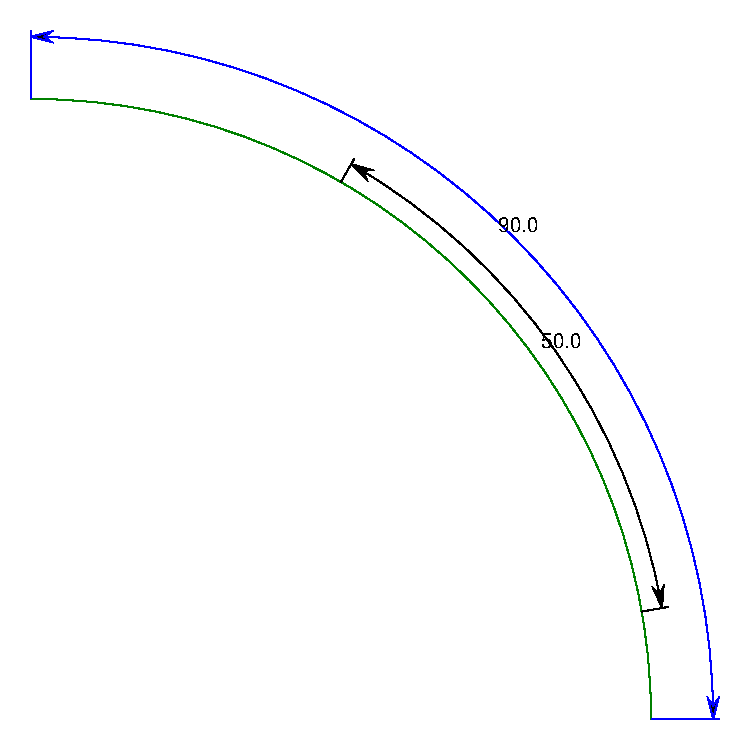
\includegraphics[width=3in,height=3in]{../images/example-angular-dimension.pdf}
\end{center}

\caption{ANGULAR-DIMENSION example}

\label{fig:ANGULAR-DIMENSION}

\end{figure}





\textbf{
\underline{Input slots (required):}}

\begin{description}

\item [Arc-object]
\index{Arc-object
[angular-dimension]}\emph{GDL object}

 The arc being measured.




\end{description}






\textbf{
\underline{Input slots (optional):}}

\begin{description}

\item [Center-point]
\index{Center-point
[angular-dimension]}\emph{3D Point}

 The center of the arc being measured.




\item [Dim-text-start]
\index{Dim-text-start
[angular-dimension]}\emph{3D Point}

 Determines where the text will start. Defaults to halfway along the arc, just beyond the radius.




\item [End-point]
\index{End-point
[angular-dimension]}\emph{3D Point}

 The end point of the arc being measured.




\item [Leader-radius]
\index{Leader-radius
[angular-dimension]}\emph{Number}

 The radius for the leader-arc.




\item [Start-point]
\index{Start-point
[angular-dimension]}\emph{3D Point}

 The start point  of the arc being measured.




\item [Text-along-leader-padding-factor]
\index{Text-along-leader-padding-factor
[angular-dimension]}\emph{Number}

 Amount of padding above leader for text-along-leader? t. This is multiplied by the
character-size to get the actual padding amount. Defaults to 1/3.




\item [Witness-1-to-center?]
\index{Witness-1-to-center?
[angular-dimension]}\emph{Boolean}

 Determines whether a witness line extends all the way from the start-point to the center.
Defaults to nil.




\item [Witness-2-to-center?]
\index{Witness-2-to-center?
[angular-dimension]}\emph{Boolean}

 Determines whether a witness line extends all the way from the end-point to the center.
Defaults to nil.




\end{description}






\textbf{
\underline{Computed slots:}}

\begin{description}

\item [Dim-value]
\index{Dim-value
[angular-dimension]}\emph{Number}

 2D distance relative to the base-plane-normal. Can be over-ridden in the subclass




\end{description}







\item \index{ARC}
\label{prim:arc}
\textbf{ARC}


\textbf{
\underline{Mixins:}} ARCOID-MIXIN, BASE-OBJECT





\begin{description}

\item [
\underline{Description}]


A segment of a circle.
The start point is at the 3 o'clock position, and positive
angles are measured anti-clockwise.



\end{description}




\begin{figure}
\begin{lrbox}{\boxedverb}
\begin{minipage}{\linewidth}
{\small

\begin{verbatim}

 (in-package :gdl-user)

 (define-object arc-sample (arc) 
   :computed-slots ((radius 30) (end-angle (half pi/2))))

 (generate-sample-drawing :objects (make-object 'arc-sample))


\end{verbatim}}
\end{minipage}
\end{lrbox}
\fbox{\usebox{\boxedverb}}

\caption{Example Code for ARC}

\label{fig:example-code-ARC}

\end{figure}

\begin{figure}
\begin{center}

\includegraphics[width=3in,height=3in]{../images/example-arc.pdf}
\end{center}

\caption{ARC example}

\label{fig:ARC}

\end{figure}





\textbf{
\underline{Input slots (required):}}

\begin{description}

\item [Radius]
\index{Radius
[arc]}\emph{Number}

 Distance from center to any point on the arc.




\end{description}






\textbf{
\underline{Input slots (optional):}}

\begin{description}

\item [End-angle]
\index{End-angle
[arc]}\emph{Angle in radians}

 End angle of the arc. Defaults to twice pi.




\item [Start-angle]
\index{Start-angle
[arc]}\emph{Angle in radians}

 Start angle of the arc. Defaults to zero.




\end{description}






\textbf{
\underline{Computed slots:}}

\begin{description}

\item [End]
\index{End
[arc]}\emph{3D Point}

 The end point of the arc.




\item [Height]
\index{Height
[arc]}\emph{Number}

 Z-axis dimension of the reference box. Defaults to zero.




\item [Length]
\index{Length
[arc]}\emph{Number}

 Y-axis dimension of the reference box. Defaults to zero.




\item [Start]
\index{Start
[arc]}\emph{3D Point}

 The start point of the arc.




\item [Width]
\index{Width
[arc]}\emph{Number}

 X-axis dimension of the reference box. Defaults to zero.




\end{description}






\textbf{
\underline{Gdl functions:}}

\begin{description}

\item [Equi-spaced-points]
\index{Equi-spaced-points
[arc]}\emph{List of points}

 Returns a list of points equally spaced around the arc, including
the start and end point of the arc.




\item [Point-on-arc]
\index{Point-on-arc
[arc]}\emph{3D Point}

 The point on the arc at a certain angle from the start.




\item [Tangent]
\index{Tangent
[arc]}\emph{3D Vector}

 Returns the tangent to the arc at the given point (which should be on the arc).




\end{description}







\item \index{ARCOID-MIXIN}
\label{prim:arcoid-mixin}
\textbf{ARCOID-MIXIN}


\textbf{
\underline{Mixins:}} VANILLA-MIXIN





\begin{description}

\item [
\underline{Description}]


This object is a low level object used to define 
an arc like object. It is not recommended to be used directly by GDL common users. 
For developers it should be used as a mixin.



\end{description}








\textbf{
\underline{Input slots (required):}}

\begin{description}

\item [Radius]
\index{Radius
[arcoid-mixin]}\emph{Number}

 Distance from center to any point on the arc.




\end{description}






\textbf{
\underline{Input slots (optional):}}

\begin{description}

\item [End-angle]
\index{End-angle
[arcoid-mixin]}\emph{Angle in radians}

 End angle of the arc. Defaults to twice pi.




\item [Start-angle]
\index{Start-angle
[arcoid-mixin]}\emph{Angle in radians}

 Start angle of the arc. Defaults to zero.




\end{description}







\item \index{BASE-COORDINATE-SYSTEM}
\label{prim:base-coordinate-system}
\textbf{BASE-COORDINATE-SYSTEM}


\textbf{
\underline{Mixins:}} BASE-OBJECT, VANILLA-MIXIN





\begin{description}

\item [
\underline{Description}]


This provides a default 3D Cartesian
   coordinate system. It mixes in base-object and does not extend it
   in any way, so as with base-object, it provides an imaginary
   geometric reference box with a length, width, height, center, and
   orientation.



\end{description}









\item \index{BASE-DRAWING}
\label{prim:base-drawing}
\textbf{BASE-DRAWING}


\textbf{
\underline{Mixins:}} BASE-OBJECT





\begin{description}

\item [
\underline{Description}]


Generic container object for displaying one or more scaled
transformed views of geometric or text-based entities. The contained views are generally 
of type \texttt{base-view}. In a GWL application-mixin, you can include one 
object of this type in the ui-display-list-leaves.

For the PDF output-format, you can also use the cad-output output-function to write the 
drawing as a PDF document. 

Since base-drawing is inherently a 2D object, only the top view (getf *standard-views* :top) 
makes sense for viewing it.



\end{description}




\begin{figure}
\begin{lrbox}{\boxedverb}
\begin{minipage}{\linewidth}
{\small

\begin{verbatim}
 (in-package :gdl-user)

 (define-object cylinder-sample (cylinder)
   :computed-slots
   ((display-controls (list :color :pink-spicy))
    (length 10)
    (radius 3)
    (number-of-sections 25)))

 (define-object base-drawing-sample (base-drawing)
  
   :objects
   ((main-view :type 'base-view
               :projection-vector (getf *standard-views* :trimetric)
               :object-roots (list (the surf)))
 
    (surf :type 'cylinder-sample
          :hidden? t))) 

 (generate-sample-drawing :objects (make-object 'base-drawing-sample))                

 
\end{verbatim}}
\end{minipage}
\end{lrbox}
\fbox{\usebox{\boxedverb}}

\caption{Example Code for BASE-DRAWING}

\label{fig:example-code-BASE-DRAWING}

\end{figure}

\begin{figure}
\begin{center}

\includegraphics[width=3in,height=3in]{../images/example-base-drawing.pdf}
\end{center}

\caption{BASE-DRAWING example}

\label{fig:BASE-DRAWING}

\end{figure}





\textbf{
\underline{Input slots (optional):}}

\begin{description}

\item [Height]
\index{Height
[base-drawing]}\emph{Number}

 Z-axis dimension of the reference box. Defaults to zero.




\item [Length]
\index{Length
[base-drawing]}\emph{Number}

 Y-axis dimension of the reference box. Defaults to zero.




\item [Page-length]
\index{Page-length
[base-drawing]}\emph{Number in PDF Points}

 Front-to-back (or top-to-bottom) length of the paper being represented
by this drawing. The default is (* 11 72) points, or 11 inches, corresponding to US standard
letter-size paper.




\item [Page-width]
\index{Page-width
[base-drawing]}\emph{Number in PDF Points}

 Left-to-right width of the paper being represented by this drawing.
The default is (* 8.5 72) points, or 8.5 inches, corresponding to US standard letter-size paper.




\item [Width]
\index{Width
[base-drawing]}\emph{Number}

 X-axis dimension of the reference box. Defaults to zero.




\end{description}







\item \index{BASE-OBJECT}
\label{prim:base-object}
\textbf{BASE-OBJECT}


\textbf{
\underline{Mixins:}} VANILLA-MIXIN





\begin{description}

\item [
\underline{Description}]


Base-Object is a superclass of most of GDL's geometric primitives. It 
provides an imaginary geometric reference box with a length, width, height, center, 
and orientation.



\end{description}




\begin{figure}
\begin{lrbox}{\boxedverb}
\begin{minipage}{\linewidth}
{\small

\begin{verbatim}

 (in-package :gdl-user)

 (define-object tower (base-object)
  
  :input-slots 
   ((number-of-blocks 50) (twist-per-block 1)
    (block-height 1) (block-width 5) (block-length 7))
  
  :objects
   ((blocks :type 'box
            :sequence (:size (the number-of-blocks))
            :center (translate (the center) 
                               :up (* (the-child index) 
                                      (the-child height)))
            :width (the block-width) 
            :height (the block-height) 
            :length (the block-length)
            :orientation (alignment 
                          :rear (if (the-child first?)
                                    (rotate-vector-d (the (face-normal-vector  :rear))
                                                     (the twist-per-block)
                                                     (the (face-normal-vector :top)))
                                    (rotate-vector-d (the-child previous 
                                                     (face-normal-vector :rear))
                                                     (the twist-per-block)
                                                     (the (face-normal-vector :top))))
                          :top (the (face-normal-vector :top))))))
;;
;;Test run
;;
#|
gdl-user(46): (setq self (make-object 'tower))
 #tower @ #x750666f2
gdl-user(47): (setq test-center (the (blocks 10) center))
#(0.0 0.0 10.0)
gdl-user(48): (the (blocks 10) (global-to-local test-center))
#(0.0 0.0 0.0)
gdl-user(49): (the (blocks 10) (local-to-global (the (blocks 10) 
                                                (global-to-local test-center))))
#(0.0 0.0 10.0)
gdl-user(50): 
gdl-user(50): (setq test-vertex (the (blocks 10) (vertex :top :right :rear)))
#(1.7862364748012536 3.9127176305081863 10.5)
gdl-user(51): (the (blocks 10) (global-to-local test-vertex))
#(2.500000000000001 3.500000000000001 0.5)
gdl-user(52): (the (blocks 10) (local-to-global (the (blocks 10) 
                                                (global-to-local test-vertex))))
#(1.786236474801254 3.9127176305081877 10.5)
gdl-user(53): 
|#
;;
;;
;;


\end{verbatim}}
\end{minipage}
\end{lrbox}
\fbox{\usebox{\boxedverb}}

\caption{Example Code for BASE-OBJECT}

\label{fig:example-code-BASE-OBJECT}

\end{figure}





\textbf{
\underline{Input slots (optional):}}

\begin{description}

\item [Bounding-box]
\index{Bounding-box
[base-object]}\emph{List of two 3D points}

 The left front bottom and right rear top corners, in global coordinates,
of the rectangular volume bounding the tree of geometric objects rooted at this object.




\item [Image-file]
\index{Image-file
[base-object]}\emph{Pathname or string}

 Points to a pre-existing image file to be displayed instead of actual geometry for this object. Defaults to nil




\item [Local-box]
\index{Local-box
[base-object]}\emph{List of two 3D points}

 The left front bottom and right rear top corners, in global coordinates,
of the rectangular volume bounding this geometric object.




\item [Obliqueness]
\index{Obliqueness
[base-object]}\emph{3x3 Orthonormal Matrix of Double-Float Numbers}

 This is synonymous with the \texttt{orientation}.




\item [Onclick-function]
\index{Onclick-function
[base-object]}\emph{Lambda function of zero arguments, or nil}

 If non-nil, this
function gets invoked when the user clicks the object in graphics
front-ends which support this functionality, e.g. SVG/Raphael and X3DOM.




\end{description}






\textbf{
\underline{Input slots (optional, defaulting):}}

\begin{description}

\item [Center]
\index{Center
[base-object]}\emph{3D Point}

 Indicates in global coordinates where the center of the reference
box of this object should be located.




\item [Display-controls]
\index{Display-controls
[base-object]}\emph{Plist}

 May contain keywords and values indicating display characteristics for
this object. The following keywords are recognized currently:



\begin{description}


\item[:color]
 color keyword from the *color-table* parameter, or an HTML-style hexidecimal
RGB string value, e.g. "\#FFFFFF" for pure white. Defaults to :black.


\item[:line-thickness]
 an integer, defaulting to 1, indicating relative line thickness for wireframe
representations of this object.


\item[:dash-pattern]
(currently PDF/PNG/JPEG only). This is a list of two or three numbers which indicate the length,
in pixels, of the dashes and blank spaces in a dashed line. The optional third number
indicates how far into the line or curve to start the dash pattern.

\end{description}





\item [Height]
\index{Height
[base-object]}\emph{Number}

 Z-axis dimension of the reference box. Defaults to zero.




\item [Length]
\index{Length
[base-object]}\emph{Number}

 Y-axis dimension of the reference box. Defaults to zero.




\item [Orientation]
\index{Orientation
[base-object]}\emph{3x3 Matrix of Double-Float Numbers}

 Indicates the absolute Rotation Matrix used to create
the coordinate system of this object. This matrix is given in absolute terms (i.e. with
respect to the root's orientation), and is generally created with the alignment function.
It should be an 
\i{orthonormal} matrix, meaning each row is a vector with a magnitude
of one (1.0).




\item [Width]
\index{Width
[base-object]}\emph{Number}

 X-axis dimension of the reference box. Defaults to zero.




\end{description}






\textbf{
\underline{Computed slots:}}

\begin{description}

\item [Color-decimal]
\index{Color-decimal
[base-object]}\emph{Vector of three real numbers}

 The RBG color of this object specified in :display-controls.
Defaults to the foreground color specified in \texttt{*colors-default*}. This message should not normally be overridden in user application code.




\item [Local-center]
\index{Local-center
[base-object]}\emph{3D Point}

 The center of this object, from the perspective of the parent. Starting
from the parent's center and using the parent's orientation, this is the relative center
of this object.




\item [Local-center*]
\index{Local-center*
[base-object]}\emph{3D Point}

 The center of this object, from the perspective of the parent. Starting
from the parent's center and using the parent's orientation, this is the relative center
of this object.




\item [Local-orientation]
\index{Local-orientation
[base-object]}\emph{3x3 Matrix of Double-Float Numbers}

 Indicates the local Rotation Matrix used
to create the coordinate system of this object. This is the ``local''
orientation with respect to the parent. Multiplying the parent's orientation
with this matrix will always result in the absolute orientation for this part.




\end{description}






\textbf{
\underline{Hidden objects:}}

\begin{description}

\item [Bounding-bbox]
\index{Bounding-bbox
[base-object]}\emph{GDL object of type Box}

 A box representing the bounding-box.




\item [Local-bbox]
\index{Local-bbox
[base-object]}\emph{GDL object of type Box}

 A box representing the local-box.




\end{description}






\textbf{
\underline{Gdl functions:}}

\begin{description}

\item [Axis-vector]
\index{Axis-vector
[base-object]}\emph{3D Vector}

 Returns the vector pointing in the positive direction of the specified axis of this object's reference box.




\item [Edge-center]
\index{Edge-center
[base-object]}\emph{3D Point}

 Returns the center of the requested edge of this object's reference box.




\item [Face-center]
\index{Face-center
[base-object]}\emph{3D Point}

 Returns the center of the requested face of this object's reference box.




\item [Face-normal-vector]
\index{Face-normal-vector
[base-object]}\emph{3D Vector}

 Returns the vector pointing from this object's reference box center to its requested face-center.




\item [Face-vertices]
\index{Face-vertices
[base-object]}\emph{List of four 3D points}

 Returns the vertices of the indicated face.




\item [Global-to-local]
\index{Global-to-local
[base-object]}\emph{3D-point}

 This function returns the point given in global coordinates, into relative local coordinates,
based on the orientation and center of the object to which the global-to-local message is sent.




\item [In-face?]
\index{In-face?
[base-object]}\emph{Boolean}

 Returns non-nil if the given point is in halfspace defined by the plane given a point and direction.




\item [Line-intersection-points]
\index{Line-intersection-points
[base-object]}\emph{List of 3D points}

 Returns the points of intersection between given line and the reference box of this object.




\item [Local-to-global]
\index{Local-to-global
[base-object]}\emph{3D-point}

 This function returns the point given in relative local coordinates, converted into global coordinates,
based on the orientation and center of the object to which the local-to-global message is sent.




\item [Vertex]
\index{Vertex
[base-object]}\emph{3D Point}

 Returns the center of the requested vertex (corner) of this object's reference box.




\end{description}







\item \index{BASE-VIEW}
\label{prim:base-view}
\textbf{BASE-VIEW}


\textbf{
\underline{Mixins:}} BASE-OBJECT





\begin{description}

\item [
\underline{Description}]


Generic container object for displaying a scaled transformed view of geometric or 
text-based objects. \texttt{Base-view} can be used by itself or as a child of a \texttt{base-drawing}

In a GWL application-mixin, you can include an object of this type in the ui-display-list-leaves.

For the PDF output-format, you can also use the cad-output output-function to write the 
view as a PDF document. 

Since base-view is inherently a 2D object, only the top view (getf *standard-views* :top) 
makes sense for viewing it.



\end{description}




\begin{figure}
\begin{lrbox}{\boxedverb}
\begin{minipage}{\linewidth}
{\small

\begin{verbatim}
                 
 (in-package :gdl-user)

 (define-object box-with-two-viewed-drawing (base-object)
  
   :objects
   ((drawing :type 'two-viewed-drawing
             :objects-to-draw (list (the box) (the length-dim)))
    
    (length-dim :type 'horizontal-dimension
                :hidden? t
                :start-point (the box (vertex :rear :top :left))
                :end-point (the box (vertex :rear :top :right)))
   
    (box :type 'box
         :hidden? t
         :length 5 :width 10 :height 15)))

 (define-object two-viewed-drawing (base-drawing)
   
   :input-slots (objects-to-draw)
   
   :objects
  
   ((main-view :type 'base-view
               :projection-vector (getf *standard-views* :trimetric)
               :length (half (the length))
               :center (translate (the center)
                                  :rear (half (the-child length)))
               :objects (the objects-to-draw))
   
    (top-view :type 'base-view
              :projection-vector (getf *standard-views* :top)
              :length (* 0.30 (the length))
              :objects (the objects-to-draw))))

   (generate-sample-drawing :objects 
    (the-object (make-object 'box-with-two-viewed-drawing) drawing top-view))
 
 
\end{verbatim}}
\end{minipage}
\end{lrbox}
\fbox{\usebox{\boxedverb}}

\caption{Example Code for BASE-VIEW}

\label{fig:example-code-BASE-VIEW}

\end{figure}

\begin{figure}
\begin{center}
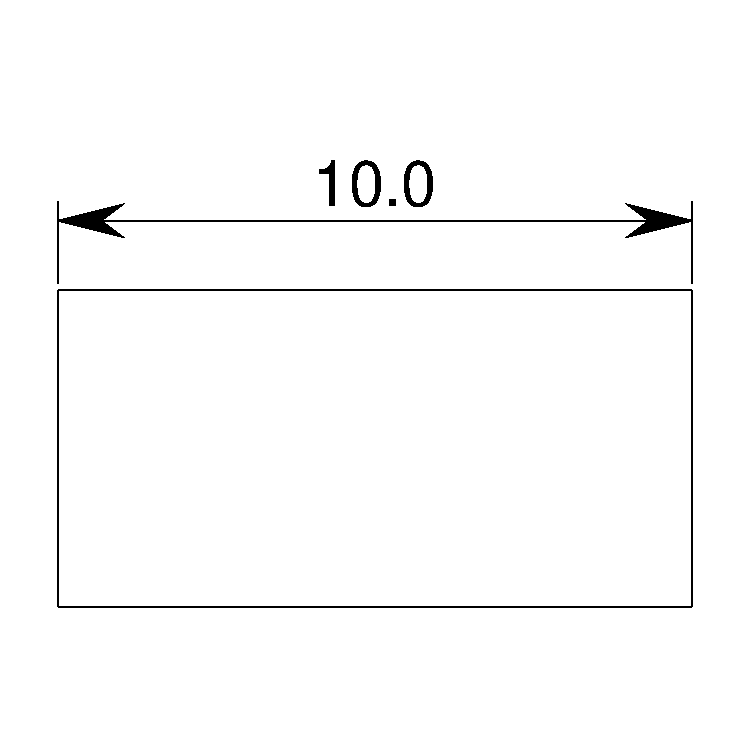
\includegraphics[width=3in,height=3in]{../images/example-base-view.pdf}
\end{center}

\caption{BASE-VIEW example}

\label{fig:BASE-VIEW}

\end{figure}





\textbf{
\underline{Input slots (optional):}}

\begin{description}

\item [Annotation-objects]
\index{Annotation-objects
[base-view]}\emph{List of GDL objects}

 These objects will be displayed in each view by default, with no scaling or transform (i.e. they are in Drawing space.




\item [Border-box?]
\index{Border-box?
[base-view]}\emph{Boolean}

 Determines whether a rectangular border box is drawn around the view,
with the view's length and width. Defaults to nil.




\item [Center]
\index{Center
[base-view]}\emph{3D-point}

 Center of the view box. Specify this or corner, not both.




\item [Corner]
\index{Corner
[base-view]}\emph{3D-point}

 Top left (i.e. rear left from top view) of the view box. Specify this or center, not both.




\item [Front-margin]
\index{Front-margin
[base-view]}\emph{Number in Drawing scale (e}

g. points). Amount of margin on front and rear
of page when \texttt{view-scale} is to be computed automatically. Defaults to 25.




\item [Immune-objects]
\index{Immune-objects
[base-view]}\emph{List of GDL objects}

 These objects are immune from view scaling and transform computations and so can freely refer
to the view-scale, view-center, and other view information for self-scaling views. Defaults to NIL.




\item [Left-margin]
\index{Left-margin
[base-view]}\emph{Number in Drawing scale (e}

g. points). Amount of margin on left and right
of page when \texttt{view-scale} is to be computed automatically. Defaults to 25.




\item [Object-roots]
\index{Object-roots
[base-view]}\emph{List of GDL objects}

 The leaves from each of these objects will be displayed in each view by default.




\item [Objects]
\index{Objects
[base-view]}\emph{List of GDL objects}

 These objects will be displayed in each view by default.




\item [Projection-vector]
\index{Projection-vector
[base-view]}\emph{3D Unitized Vector}

 Direction of camera pointing to model (the object-roots and/or the objects) to create
this view. The view is automatically ``twisted''about this vector to result in ``up'' being as close as
possible to the Z vector, unless this vector is parallel to the Z vector in which case ``up'' is taken
to be the Y (rear) vector. This vector is normally taken from the \texttt{*standard-views*} built-in GDL
parameter. Defaults to \texttt{(getf *standard-views* :top)}, which is the vector [0, 0, 1].




\item [Snap-to]
\index{Snap-to
[base-view]}\emph{3D Vector}

 For a top view, this vector specifies the direction that the rear of
the box should be facing. Defaults to \texttt{*nominal-y-vector*}.




\item [View-center]
\index{View-center
[base-view]}\emph{3D Point in Model space}

 Point relative to each object's center to use as center of the view.




\item [View-scale]
\index{View-scale
[base-view]}\emph{Number}

 Ratio of drawing scale (in points) to model scale for this view. Defaults to being auto-computed.




\end{description}






\textbf{
\underline{Gdl functions:}}

\begin{description}

\item [Model-point]
\index{Model-point
[base-view]}\emph{3D Point}

 Takes point in view coordinates and returns corresponding point in model coordinates.




\item [View-point]
\index{View-point
[base-view]}\emph{3D Point}

 Takes point in model coordinates and returns corresponding point in view coordinates.




\end{description}







\item \index{BEZIER-CURVE}
\label{prim:bezier-curve}
\textbf{BEZIER-CURVE}


\textbf{
\underline{Mixins:}} BASE-OBJECT





\begin{description}

\item [
\underline{Description}]


GDL currently supports third-degree Bezier curves, which are 
defined using four 3D 
\i{control-points}. The Bezier curve always passes 
through the first and last control points and lies within the convex hull of the control 
points. At the start point (i.e. the first control point), the curve is tangent 
to the vector pointing from the start point to the second control point. 
At the end point (i.e. the last control point), the curve is tangent to the 
vector pointing from the end point to the third control point.



\end{description}




\begin{figure}
\begin{lrbox}{\boxedverb}
\begin{minipage}{\linewidth}
{\small

\begin{verbatim}
 (in-package :gdl-user)

 (define-object bezier-sample (bezier-curve)
  :computed-slots
  ((control-points (list (make-point 0 0 0)
                         (make-point 1 1 0)
                         (make-point 2 1 0)
                         (make-point 3 0 0))))
  :objects
  ((points-display :type 'points-display
                   :points (the control-points))))

 (generate-sample-drawing :objects (let ((self (make-object 'bezier-sample)))
                                     (list self (the points-display))))

\end{verbatim}}
\end{minipage}
\end{lrbox}
\fbox{\usebox{\boxedverb}}

\caption{Example Code for BEZIER-CURVE}

\label{fig:example-code-BEZIER-CURVE}

\end{figure}

\begin{figure}
\begin{center}
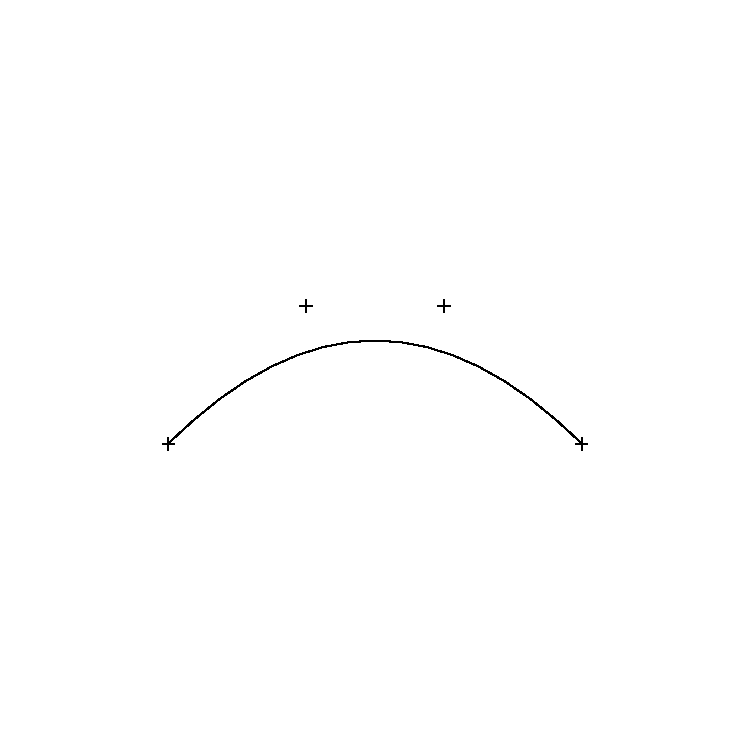
\includegraphics[width=3in,height=3in]{../images/example-bezier-curve.pdf}
\end{center}

\caption{BEZIER-CURVE example}

\label{fig:BEZIER-CURVE}

\end{figure}





\textbf{
\underline{Input slots (required):}}

\begin{description}

\item [Control-points]
\index{Control-points
[bezier-curve]}\emph{List of 4 3D Points}

 Specifies the control points for the Bezier curve.




\end{description}






\textbf{
\underline{Computed slots:}}

\begin{description}

\item [Bounding-box]
\index{Bounding-box
[bezier-curve]}\emph{List of two 3D points}

 The left front bottom and right rear top corners, in global coordinates,
of the rectangular volume bounding the tree of geometric objects rooted at this object.




\end{description}






\textbf{
\underline{Gdl functions:}}

\begin{description}

\item [Circle-intersection-2d]
\index{Circle-intersection-2d
[bezier-curve]}\emph{List of 3D points}

 Returns points of intersection in the Z plane between this Bezier curve and
the circle in the Z plane with center \texttt{center} and radius \texttt{radius}.




\item [Line-intersection-2d]
\index{Line-intersection-2d
[bezier-curve]}\emph{List of 3D points}

 Returns points of intersection in the Z plane between this Bezier curve
and the infinite line containing point \texttt{point} and direction \texttt{vector}. Use the
between? function if you wish to establish whether the point is contained in a particular line
segment.




\item [Point]
\index{Point
[bezier-curve]}\emph{3D Point}

 Returns the point on this Bezier curve corresponding to the given \texttt{parameter},
which should be between 0 and 1.




\end{description}







\item \index{BOX}
\label{prim:box}
\textbf{BOX}


\textbf{
\underline{Mixins:}} BASE-OBJECT





\begin{description}

\item [
\underline{Description}]


This represents a ``visible'' base-object -- a six-sided box with all the same
messages as base-object, which knows how to output itself in various formats.



\end{description}




\begin{figure}
\begin{lrbox}{\boxedverb}
\begin{minipage}{\linewidth}
{\small

\begin{verbatim}
 (in-package :gdl-user)

 (define-object box-sample (box)
   :computed-slots ((display-controls (list :color :blue-neon))
                    (length 10)
                    (width (* (the length) +phi+))
                    (height (* (the width) +phi+))))

 (generate-sample-drawing :objects (make-object 'box-sample)
                          :projection-direction (getf *standard-views* :trimetric))


\end{verbatim}}
\end{minipage}
\end{lrbox}
\fbox{\usebox{\boxedverb}}

\caption{Example Code for BOX}

\label{fig:example-code-BOX}

\end{figure}

\begin{figure}
\begin{center}
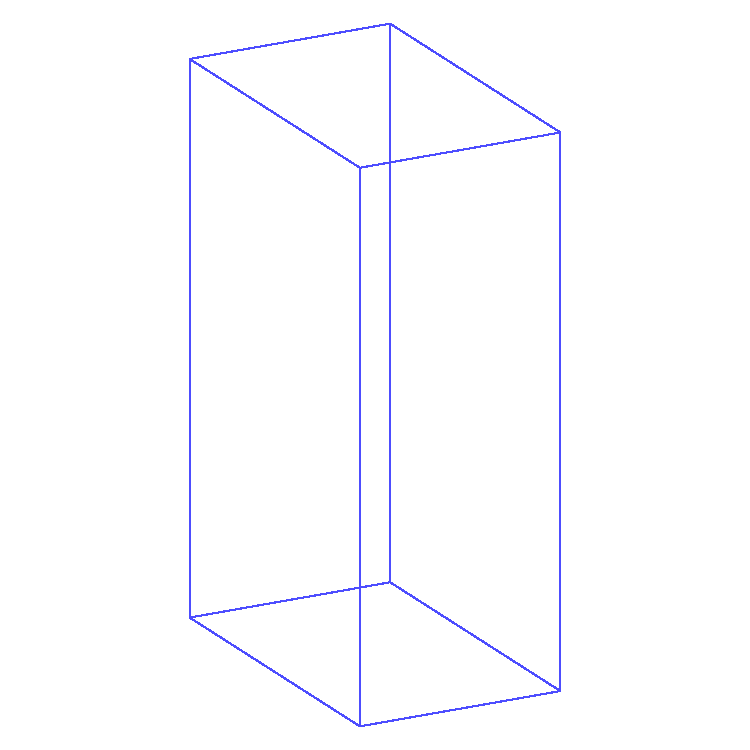
\includegraphics[width=3in,height=3in]{../images/example-box.pdf}
\end{center}

\caption{BOX example}

\label{fig:BOX}

\end{figure}





\textbf{
\underline{Computed slots:}}

\begin{description}

\item [Volume]
\index{Volume
[box]}\emph{Number}

 Total volume of the box.




\end{description}







\item \index{C-CYLINDER}
\label{prim:c-cylinder}
\textbf{C-CYLINDER}


\textbf{
\underline{Mixins:}} CYLINDER





\begin{description}

\item [
\underline{Description}]


Provides a simple way to create a cylinder, by specifying a start point and an end point.



\end{description}




\begin{figure}
\begin{lrbox}{\boxedverb}
\begin{minipage}{\linewidth}
{\small

\begin{verbatim}

 (in-package :gdl-user)

 (define-object c-cylinder-sample (c-cylinder)
   :computed-slots
   ((display-controls (list :color :plum :transparency 0.2))
    (start (make-point 0 0 0))
    (end (make-point 0 0 10))
    (number-of-sections 7)
    (radius 3)))

   (generate-sample-drawing :objects (make-object 'c-cylinder-sample)
                            :projection-direction (getf *standard-views* :trimetric))
   


\end{verbatim}}
\end{minipage}
\end{lrbox}
\fbox{\usebox{\boxedverb}}

\caption{Example Code for C-CYLINDER}

\label{fig:example-code-C-CYLINDER}

\end{figure}

\begin{figure}
\begin{center}
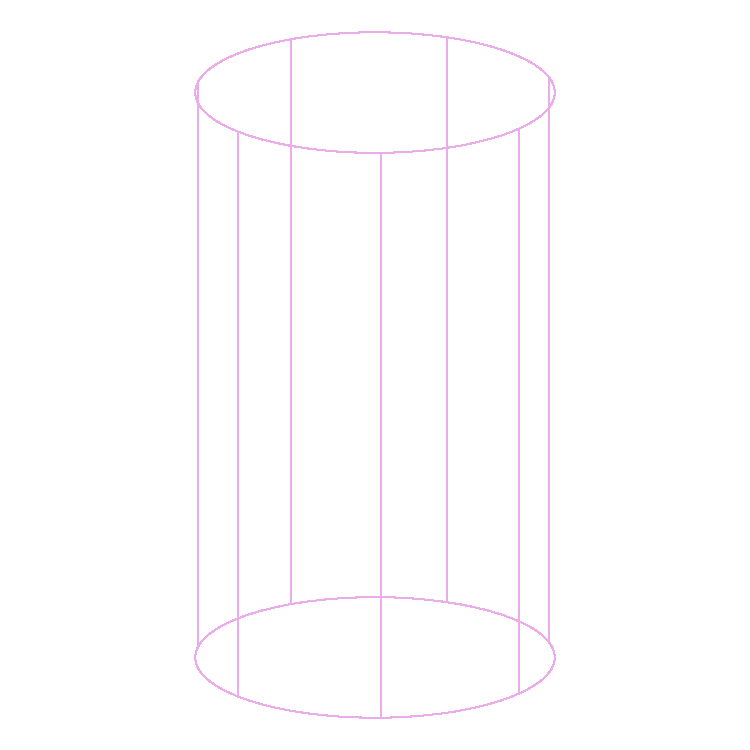
\includegraphics[width=3in,height=3in]{../images/example-c-cylinder.pdf}
\end{center}

\caption{C-CYLINDER example}

\label{fig:C-CYLINDER}

\end{figure}





\textbf{
\underline{Input slots (required):}}

\begin{description}

\item [End]
\index{End
[c-cylinder]}\emph{3D Point}

 Center of the end cap.




\item [Start]
\index{Start
[c-cylinder]}\emph{3D Point}

 Center of the start cap.




\end{description}






\textbf{
\underline{Computed slots:}}

\begin{description}

\item [Center]
\index{Center
[c-cylinder]}\emph{3D Point}

 Center point of the center-line.




\item [Center-line]
\index{Center-line
[c-cylinder]}\emph{List of two 3D Points}

 Represents line segment connecting center of end cap to center of start cap.




\item [Length]
\index{Length
[c-cylinder]}\emph{Number}

 Distance between cap centers.




\item [Orientation]
\index{Orientation
[c-cylinder]}\emph{3x3 Orthonormal Rotation Matrix}

 Resultant orientation given the specified start and end points.




\end{description}







\item \index{CENTER-LINE}
\label{prim:center-line}
\textbf{CENTER-LINE}


\textbf{
\underline{Mixins:}} OUTLINE-SPECIALIZATION-MIXIN, BASE-OBJECT





\begin{description}

\item [
\underline{Description}]


Creates a dashed single centerline or crosshair centerline on a circle.



\end{description}




\begin{figure}
\begin{lrbox}{\boxedverb}
\begin{minipage}{\linewidth}
{\small

\begin{verbatim}
 (in-package :gdl-user)

 (define-object center-line-test (base-object)
 
  :objects 
  ((circle-sample :type 'circle
                  :display-controls (list :color :green)
                  :center (make-point 10 10 10 )
                  :radius 10)
   
   (center-line-sample :type 'center-line
                       :circle? t
                       :center (the circle-sample center)
                       :size (* 2.1 (the circle-sample radius)))))

  (generate-sample-drawing 
  :objects (list 
            (the-object (make-object 'center-line-test) 
                        circle-sample) 
            (the-object (make-object 'center-line-test) 
                        center-line-sample))
  :projection-direction (getf *standard-views* :top))
 
 
\end{verbatim}}
\end{minipage}
\end{lrbox}
\fbox{\usebox{\boxedverb}}

\caption{Example Code for CENTER-LINE}

\label{fig:example-code-CENTER-LINE}

\end{figure}

\begin{figure}
\begin{center}
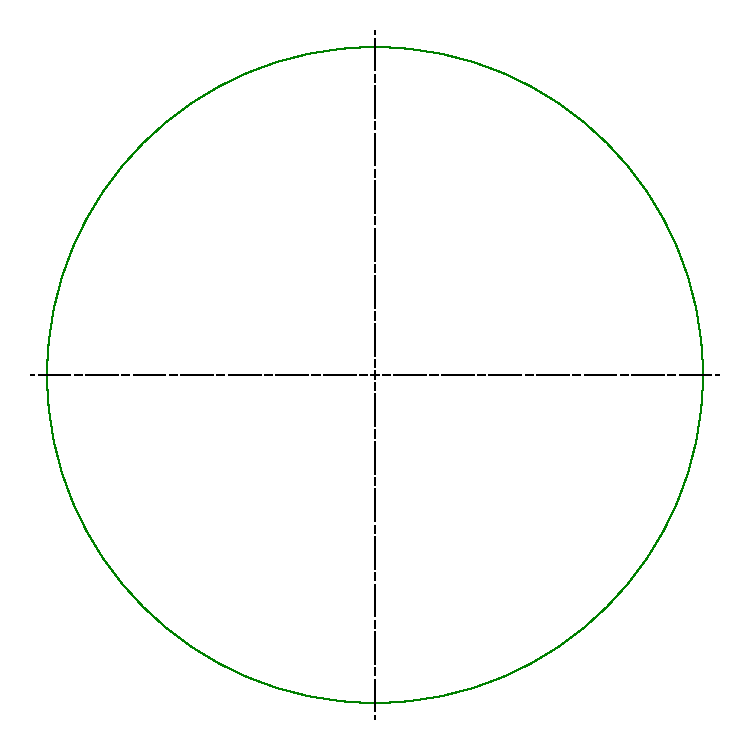
\includegraphics[width=3in,height=3in]{../images/example-center-line.pdf}
\end{center}

\caption{CENTER-LINE example}

\label{fig:CENTER-LINE}

\end{figure}





\textbf{
\underline{Input slots (required):}}

\begin{description}

\item [Size]
\index{Size
[center-line]}\emph{Number}

 The length of the centerline.




\end{description}






\textbf{
\underline{Input slots (optional):}}

\begin{description}

\item [Circle?]
\index{Circle?
[center-line]}\emph{Boolean}

 Determines whether this will be a circle crosshair. Defaults to nil.




\end{description}






\textbf{
\underline{Input slots (optional, defaulting):}}

\begin{description}

\item [Gap-length]
\index{Gap-length
[center-line]}\emph{Number}

 Distance between dashed line segments. Defaults to 0.1.




\item [Long-segment-length]
\index{Long-segment-length
[center-line]}\emph{Number}

 Length of longer dashed line segments. Defaults to 1.0.




\item [Short-segment-length]
\index{Short-segment-length
[center-line]}\emph{Number}

 Length of shorter dashed line segments. Defaults to 0.25.




\end{description}






\textbf{
\underline{Computed slots:}}

\begin{description}

\item [Height]
\index{Height
[center-line]}\emph{Number}

 Z-axis dimension of the reference box. Defaults to zero.




\item [Length]
\index{Length
[center-line]}\emph{Number}

 Y-axis dimension of the reference box. Defaults to zero.




\item [Width]
\index{Width
[center-line]}\emph{Number}

 X-axis dimension of the reference box. Defaults to zero.




\end{description}







\item \index{CIRCLE}
\label{prim:circle}
\textbf{CIRCLE}


\textbf{
\underline{Mixins:}} ARC





\begin{description}

\item [
\underline{Description}]


The set of points equidistant from a given point. 
The distance from the center is called the radius, and the point is called 
the center. The start point of the circle is at the 3 o'clock position, and positive
angles are measured anti-clockwise.



\end{description}




\begin{figure}
\begin{lrbox}{\boxedverb}
\begin{minipage}{\linewidth}
{\small

\begin{verbatim}

  (in-package :gdl-user)
                  
  (define-object circle-sample (circle)
    :computed-slots
    ((radius 10)))

  (generate-sample-drawing :objects (make-object 'circle-sample))

                  

\end{verbatim}}
\end{minipage}
\end{lrbox}
\fbox{\usebox{\boxedverb}}

\caption{Example Code for CIRCLE}

\label{fig:example-code-CIRCLE}

\end{figure}

\begin{figure}
\begin{center}

\includegraphics[width=3in,height=3in]{../images/example-circle.pdf}
\end{center}

\caption{CIRCLE example}

\label{fig:CIRCLE}

\end{figure}





\textbf{
\underline{Computed slots:}}

\begin{description}

\item [Area]
\index{Area
[circle]}\emph{Number}

 The area enclosed by the circle.




\item [Circumference]
\index{Circumference
[circle]}\emph{Number}

 The perimeter of the circle.




\item [End-angle]
\index{End-angle
[circle]}\emph{Angle in radians}

 End angle of the arc. Defaults to twice pi.




\item [Start-angle]
\index{Start-angle
[circle]}\emph{Angle in radians}

 Start angle of the arc. Defaults to zero.




\end{description}







\item \index{CONE}
\label{prim:cone}
\textbf{CONE}


\textbf{
\underline{Mixins:}} CYLINDER





\begin{description}

\item [
\underline{Description}]


A pyramid with a circular cross section, with its vertex above 
the center of its base. Partial cones and hollow cones are supported.



\end{description}




\begin{figure}
\begin{lrbox}{\boxedverb}
\begin{minipage}{\linewidth}
{\small

\begin{verbatim}
  (in-package :gdl-user)

   (define-object cone-sample (cone)
     :computed-slots
     ((display-controls (list :color :blue-neon 
                              :transparency 0.5 
                              :shininess 0.8 
                              :specular-color :white))
      (length 10) (radius-1 2)(inner-radius-1 1)
      (radius-2 5) (number-of-sections 5)
      (inner-radius-2 3)))
  
 (generate-sample-drawing :objects (make-object 'cone-sample) 
                          :projection-direction :trimetric) 
  
\end{verbatim}}
\end{minipage}
\end{lrbox}
\fbox{\usebox{\boxedverb}}

\caption{Example Code for CONE}

\label{fig:example-code-CONE}

\end{figure}

\begin{figure}
\begin{center}
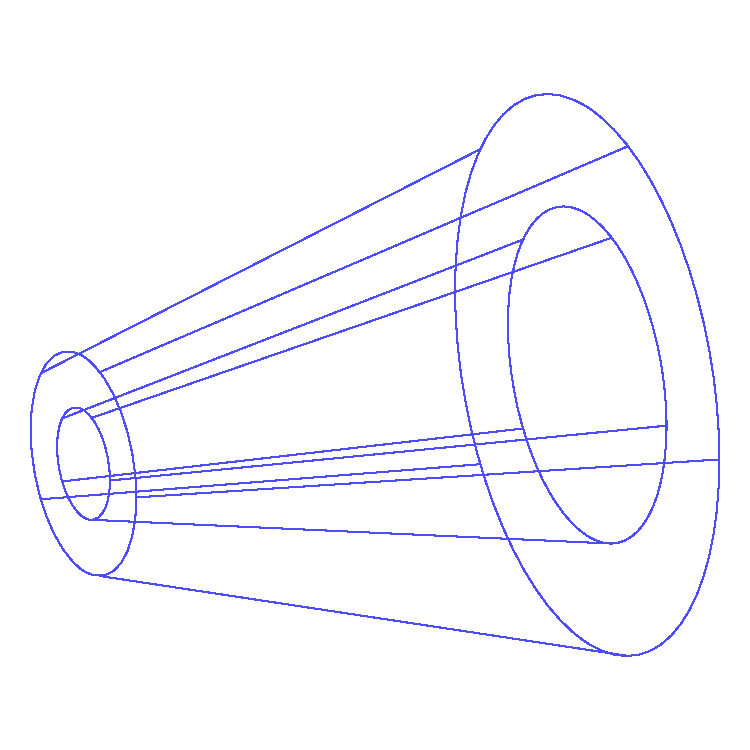
\includegraphics[width=3in,height=3in]{../images/example-cone.pdf}
\end{center}

\caption{CONE example}

\label{fig:CONE}

\end{figure}





\textbf{
\underline{Input slots (optional):}}

\begin{description}

\item [Inner-radius-1]
\index{Inner-radius-1
[cone]}\emph{Number}

 The radius of the inner hollow part at the top end for a hollow cone.




\item [Inner-radius-2]
\index{Inner-radius-2
[cone]}\emph{Number}

 The radius of the inner hollow part at the bottom end for a hollow cone.




\item [Radius-1]
\index{Radius-1
[cone]}\emph{Number}

 The radius of the top end of the cone.




\item [Radius-2]
\index{Radius-2
[cone]}\emph{Number}

 The radius of the bottom end of the cone.




\end{description}






\textbf{
\underline{Computed slots:}}

\begin{description}

\item [Height]
\index{Height
[cone]}\emph{Number}

 Z-axis dimension of the reference box. Defaults to zero.




\item [Width]
\index{Width
[cone]}\emph{Number}

 X-axis dimension of the reference box. Defaults to zero.




\end{description}







\item \index{CONSTRAINED-ARC}
\label{prim:constrained-arc}
\textbf{CONSTRAINED-ARC}


\textbf{
\underline{Mixins:}} ARC





\begin{description}

\item [
\underline{Description}]


This object is intended to simplify the process of
   constructing lines using various constraints. Currently supported
   are 2 through-points or 1 through-point and at-angle. Note the
   line-constraints must be an evaluatable s-expression as this is not
   processed as a macro



\end{description}








\textbf{
\underline{Computed slots:}}

\begin{description}

\item [Center]
\index{Center
[constrained-arc]}\emph{3D Point}

 Indicates in global coordinates where the center of the reference
box of this object should be located.




\item [Orientation]
\index{Orientation
[constrained-arc]}\emph{3x3 Matrix of Double-Float Numbers}

 Indicates the absolute Rotation Matrix used to create
the coordinate system of this object. This matrix is given in absolute terms (i.e. with
respect to the root's orientation), and is generally created with the alignment function.
It should be an 
\i{orthonormal} matrix, meaning each row is a vector with a magnitude
of one (1.0).




\item [Radius]
\index{Radius
[constrained-arc]}\emph{Number}

 Distance from center to any point on the arc.




\end{description}







\item \index{CONSTRAINED-FILLET}
\label{prim:constrained-fillet}
\textbf{CONSTRAINED-FILLET}


\textbf{
\underline{Mixins:}} CONSTRAINED-ARC, VANILLA-MIXIN





\begin{description}

\item [
\underline{Description}]


This object is the same as constrained-arc, but it is only
meaningful for arc-constraints which contain two :tangent-to clauses,
and it automatically trims the result to each point of tangency



\end{description}








\textbf{
\underline{Computed slots:}}

\begin{description}

\item [End-angle]
\index{End-angle
[constrained-fillet]}\emph{Angle in radians}

 End angle of the arc. Defaults to twice pi.




\item [Start-angle]
\index{Start-angle
[constrained-fillet]}\emph{Angle in radians}

 Start angle of the arc. Defaults to zero.




\end{description}







\item \index{CONSTRAINED-LINE}
\label{prim:constrained-line}
\textbf{CONSTRAINED-LINE}


\textbf{
\underline{Mixins:}} LINE





\begin{description}

\item [
\underline{Description}]


This object is intended to simplify the process of
   constructing lines using various constraints. Currently supported
   are 2 through-points or 1 through-point and at-angle. Note the
   line-constraints must be an evaluatable s-expression as this is not
   processed as a macro



\end{description}








\textbf{
\underline{Computed slots:}}

\begin{description}

\item [End]
\index{End
[constrained-line]}\emph{3D Point}

 The end point of the line, in global coordinates.




\item [Start]
\index{Start
[constrained-line]}\emph{3D Point}

 The start point of the line, in global coordinates.




\end{description}






\textbf{
\underline{Gdl functions:}}

\begin{description}

\item [Tangent-point]
\index{Tangent-point
[constrained-line]}

Icad Compat function




\end{description}







\item \index{CYLINDER}
\label{prim:cylinder}
\textbf{CYLINDER}


\textbf{
\underline{Mixins:}} IFS-OUTPUT-MIXIN, ARCOID-MIXIN, BASE-OBJECT





\begin{description}

\item [
\underline{Description}]


An extrusion of circular cross section in which the 
centers of the circles all lie on a single line (i.e., a right circular cylinder).
Partial cylinders and hollow cylinders are supported.



\end{description}




\begin{figure}
\begin{lrbox}{\boxedverb}
\begin{minipage}{\linewidth}
{\small

\begin{verbatim}

 (in-package :gdl-user)

 (define-object cylinder-sample (cylinder)
   :computed-slots
   ((display-controls (list :color :pink-spicy))
    (length 10)
    (radius 3)
    (number-of-sections 25)))


 (generate-sample-drawing :objects (make-object 'cylinder-sample)
                          :projection-direction (getf *standard-views* :trimetric))
   


\end{verbatim}}
\end{minipage}
\end{lrbox}
\fbox{\usebox{\boxedverb}}

\caption{Example Code for CYLINDER}

\label{fig:example-code-CYLINDER}

\end{figure}

\begin{figure}
\begin{center}

\includegraphics[width=3in,height=3in]{../images/example-cylinder.pdf}
\end{center}

\caption{CYLINDER example}

\label{fig:CYLINDER}

\end{figure}





\textbf{
\underline{Input slots (required):}}

\begin{description}

\item [Length]
\index{Length
[cylinder]}\emph{Number}

 Distance from center of start cap to center of end cap.




\item [Radius]
\index{Radius
[cylinder]}\emph{Number}

 Radius of the circular cross section of the cylinder.




\end{description}






\textbf{
\underline{Input slots (optional):}}

\begin{description}

\item [Bottom-cap?]
\index{Bottom-cap?
[cylinder]}\emph{Boolean}

 Determines whether to include bottom cap in shaded renderings. Defaults to T.




\item [Closed?]
\index{Closed?
[cylinder]}\emph{Boolean}

 Indicates that a partial cylinder (or cone) should have a closed gap.




\item [Height]
\index{Height
[cylinder]}\emph{Number}

 Z-axis dimension of the reference box. Defaults to zero.




\item [Inner-radius]
\index{Inner-radius
[cylinder]}\emph{Number}

 Radius of the hollow inner portion for a hollow cylinder.




\item [Number-of-sections]
\index{Number-of-sections
[cylinder]}\emph{Integer}

 Number of vertical sections to be drawn in wireframe rendering mode.




\item [Top-cap?]
\index{Top-cap?
[cylinder]}\emph{Boolean}

 Determines whether to include bottom cap in shaded renderings. Defaults to T.




\item [Width]
\index{Width
[cylinder]}\emph{Number}

 X-axis dimension of the reference box. Defaults to zero.




\end{description}






\textbf{
\underline{Computed slots:}}

\begin{description}

\item [Direction-vector]
\index{Direction-vector
[cylinder]}\emph{3D Vector}

 Points from the start to the end.




\item [End]
\index{End
[cylinder]}\emph{3D Point}

 The center of the end cap.




\item [Hollow?]
\index{Hollow?
[cylinder]}\emph{Boolean}

 Indicates whether there is an inner-radius and thus the cylinder is hollow.




\item [Start]
\index{Start
[cylinder]}\emph{3D Point}

 The center of the start cap.




\end{description}







\item \index{ELLIPSE}
\label{prim:ellipse}
\textbf{ELLIPSE}


\textbf{
\underline{Mixins:}} ARCOID-MIXIN, BASE-OBJECT





\begin{description}

\item [
\underline{Description}]


A curve which is the locus of all points in the plane 
the sum of whose distances from two fixed points (the foci) is a given positive constant.
This is a simplified 3D ellipse which will snap to the nearest quarter if you make it a 
partial ellipse. For a full ellipse, do not specify start-angle or end-angle.



\end{description}




\begin{figure}
\begin{lrbox}{\boxedverb}
\begin{minipage}{\linewidth}
{\small

\begin{verbatim}
  
  (in-package :gdl-user)

  (define-object ellipse-sample (ellipse)
    :computed-slots
    ((minor-axis-length 10)
     (major-axis-length (* (the minor-axis-length) +phi+))
     (start-angle 0)
     (end-angle pi)))

  (generate-sample-drawing :objects (make-object 'ellipse-sample))
  
  
\end{verbatim}}
\end{minipage}
\end{lrbox}
\fbox{\usebox{\boxedverb}}

\caption{Example Code for ELLIPSE}

\label{fig:example-code-ELLIPSE}

\end{figure}

\begin{figure}
\begin{center}

\includegraphics[width=3in,height=3in]{../images/example-ellipse.pdf}
\end{center}

\caption{ELLIPSE example}

\label{fig:ELLIPSE}

\end{figure}





\textbf{
\underline{Input slots (required):}}

\begin{description}

\item [Major-axis-length]
\index{Major-axis-length
[ellipse]}\emph{Number}

 Length of (generally) the longer ellipse axis




\item [Minor-axis-length]
\index{Minor-axis-length
[ellipse]}\emph{Number}

 Length of (generally) the shorter ellipse axis




\end{description}






\textbf{
\underline{Input slots (optional):}}

\begin{description}

\item [End-angle]
\index{End-angle
[ellipse]}\emph{Angle in Radians}

 End angle of the ellipse. Defaults to 2pi for full ellipse.




\item [Start-angle]
\index{Start-angle
[ellipse]}\emph{Angle in Radians}

 Start angle of the ellipse. Defaults to 0 for full ellipse.




\end{description}






\textbf{
\underline{Computed slots:}}

\begin{description}

\item [Height]
\index{Height
[ellipse]}\emph{Number}

 Z-axis dimension of the reference box. Defaults to zero.




\item [Length]
\index{Length
[ellipse]}\emph{Number}

 Y-axis dimension of the reference box. Defaults to zero.




\item [Width]
\index{Width
[ellipse]}\emph{Number}

 X-axis dimension of the reference box. Defaults to zero.




\end{description}







\item \index{GENERAL-NOTE}
\label{prim:general-note}
\textbf{GENERAL-NOTE}


\textbf{
\underline{Mixins:}} OUTLINE-SPECIALIZATION-MIXIN, BASE-OBJECT





\begin{description}

\item [
\underline{Description}]


Creates a text note in the graphical view port and in a PDF DXF output file.



\end{description}




\begin{figure}
\begin{lrbox}{\boxedverb}
\begin{minipage}{\linewidth}
{\small

\begin{verbatim} 
 (in-package :gdl-user)

 (define-object general-note-test (base-object)
  
  :computed-slots
  
  ((blocks-note 
   (list
    "David Brown" "Created by" "ABC 2"
    "Jane Smith" "Approved by" "CCD 2"))
   (blocks-center 
    (list '(-15  5 0) '(-40  5 0) '(-55  5 0)
          '(-15 15 0) '(-40 15 0) '(-55 15 0)))
   (blocks-width (list 30 20 10 30 20 10)))
  
  :objects 
  
  ((title-block :type 'box
                :sequence (:size (length (the blocks-center)))
                :display-controls (list :color :red)
                :center (apply-make-point 
                         (nth (the-child index ) 
                              (the blocks-center)))
                :length 10
                :width (nth (the-child index ) 
                            (the blocks-width))
                :height 0)

   (general-note-sample :type 'general-note
                        :sequence (:size (length (the blocks-note)))
                        :center (the (title-block 
                                      (the-child index)) center)
                        :character-size 2.5
                        :strings (nth (the-child index) 
                                      (the blocks-note)))))
  (generate-sample-drawing 
  :objects (list-elements (make-object 'general-note-test)) 
  :projection-direction (getf *standard-views* :top))


\end{verbatim}}
\end{minipage}
\end{lrbox}
\fbox{\usebox{\boxedverb}}

\caption{Example Code for GENERAL-NOTE}

\label{fig:example-code-GENERAL-NOTE}

\end{figure}

\begin{figure}
\begin{center}
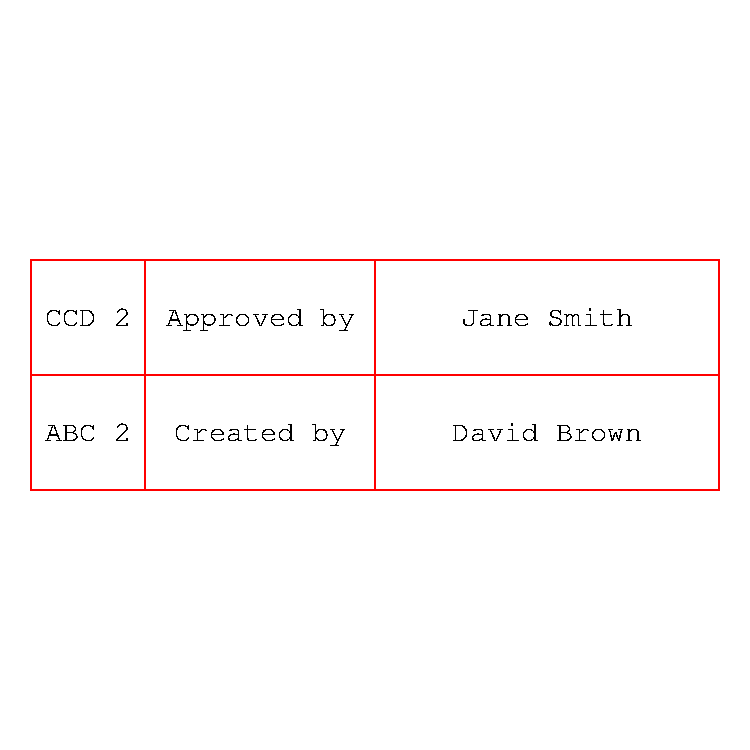
\includegraphics[width=3in,height=3in]{../images/example-general-note.pdf}
\end{center}

\caption{GENERAL-NOTE example}

\label{fig:GENERAL-NOTE}

\end{figure}





\textbf{
\underline{Input slots (optional):}}

\begin{description}

\item [Center]
\index{Center
[general-note]}\emph{3D-point}

 Center of the text. Specify this or start, not both.




\item [Character-size]
\index{Character-size
[general-note]}\emph{Number}

 Specifies the character size in drawing units.




\item [Dxf-font]
\index{Dxf-font
[general-note]}\emph{String}

 This names the DXF font for this general-note. Defaults to \texttt{(the font)}.




\item [Dxf-offset]
\index{Dxf-offset
[general-note]}\emph{Number}

 The start of text will be offset by this amount for DXF output. Default is 0.




\item [Dxf-size-ratio]
\index{Dxf-size-ratio
[general-note]}\emph{Number}

 The scale factor for DXF character size vs PDF character size. Default is 0.8




\item [Dxf-text-x-scale]
\index{Dxf-text-x-scale
[general-note]}\emph{Number in Percentage}

 Adjusts the character width for DXF output. Defaults to the text-x-scale.




\item [Font]
\index{Font
[general-note]}\emph{String}

 The font for PDF. Possibilities for built-in PDF fonts are:


\begin{itemize}

\item courier

\item courier-bold

\item courier-boldoblique

\item courier-oblique

\item helvetica

\item helvetica-bold

\item helvetica-boldoblique

\item helvetica-oblique

\item symbol

\item times-roman

\item times-bold

\item times-bolditalic

\item times-italic

\item zapfdingbats

\end{itemize}


Defaults to "Courier".




\item [Height]
\index{Height
[general-note]}\emph{Number}

 Z-axis dimension of the reference box. Defaults to zero.




\item [Justification]
\index{Justification
[general-note]}\emph{Keyword symbol, :left, :right, or :center}

 Justifies text with its box. Default is :left.




\item [Leading]
\index{Leading
[general-note]}\emph{Number}

 Space between lines of text. Default is 1.2 times the character size.




\item [Length]
\index{Length
[general-note]}\emph{Number}

 Y-axis dimension of the reference box. Defaults to zero.




\item [Outline-shape-type]
\index{Outline-shape-type
[general-note]}\emph{Keyword symbol}

 Currently can be :bubble, :rectangle, or :none. Default is :none.




\item [Start]
\index{Start
[general-note]}\emph{3D-point}

 Start of the text. Specify this or center, not both.




\item [Strings]
\index{Strings
[general-note]}\emph{List of Strings}

 The text to be displayed in the note.




\item [Text-x-scale]
\index{Text-x-scale
[general-note]}\emph{Number in Percentage}

 Adjusts the character width for PDF output. Defaults to 100.




\item [Underline?]
\index{Underline?
[general-note]}\emph{Boolean}

 Determines whether text is underlined.




\item [Width]
\index{Width
[general-note]}\emph{Number}

 Determines the width of the containing box. Default is the maximum-text-width.




\end{description}






\textbf{
\underline{Computed slots:}}

\begin{description}

\item [Maximum-text-width]
\index{Maximum-text-width
[general-note]}\emph{Number}

 Convienence computation giving the maximum input width required to keep one line per string




\end{description}







\item \index{GLOBAL-FILLETED-POLYGON-PROJECTION}
\label{prim:global-filleted-polygon-projection}
\textbf{GLOBAL-FILLETED-POLYGON-PROJECTION}


\textbf{
\underline{Mixins:}} GLOBAL-POLYGON-PROJECTION





\begin{description}

\item [
\underline{Description}]


Similar to a global-polygon-projection, but the polygon is filleted
as with global-filleted-polygon.



\end{description}




\begin{figure}
\begin{lrbox}{\boxedverb}
\begin{minipage}{\linewidth}
{\small

\begin{verbatim}
 (in-package :gdl-user)

 (define-object global-filleted-polygon-projection-sample 
     (global-filleted-polygon-projection)
     :computed-slots
     ((display-controls (list :color :blue-steel 
                              :transparency 0.3 
                              :shininess 0.7 
                              :spectral-color :white))
      (default-radius 5)
      (projection-depth 5)
      (vertex-list (list (make-point 0 0 0)
                         (make-point 10 10 0)
                         (make-point 30 10 0)
                         (make-point 40 0 0)
                         (make-point 30 -10 0)
                         (make-point 10 -10 0)
                         (make-point 0 0 0)))))

 (generate-sample-drawing :objects 
                          (make-object 'global-filleted-polygon-projection-sample)
                          :projection-direction :trimetric)






\end{verbatim}}
\end{minipage}
\end{lrbox}
\fbox{\usebox{\boxedverb}}

\caption{Example Code for GLOBAL-FILLETED-POLYGON-PROJECTION}

\label{fig:example-code-GLOBAL-FILLETED-POLYGON-PROJECTION}

\end{figure}

\begin{figure}
\begin{center}
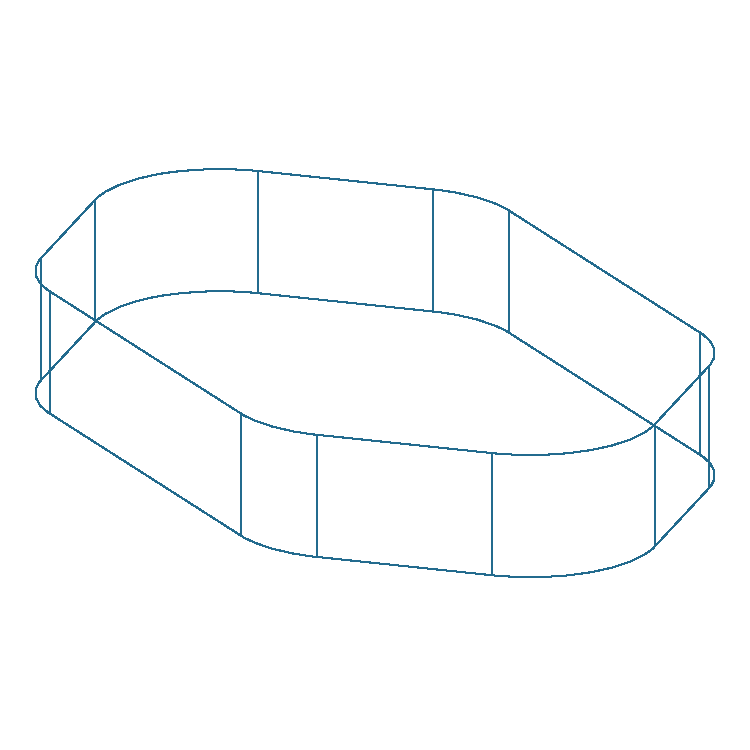
\includegraphics[width=3in,height=3in]{../images/example-global-filleted-polygon-projection.pdf}
\end{center}

\caption{GLOBAL-FILLETED-POLYGON-PROJECTION example}

\label{fig:GLOBAL-FILLETED-POLYGON-PROJECTION}

\end{figure}





\textbf{
\underline{Input slots (optional):}}

\begin{description}

\item [Default-radius]
\index{Default-radius
[global-filleted-polygon-projection]}\emph{Number}

 Specifies a radius to use for all vertices. Radius-list will take precedence over this.




\item [Radius-list]
\index{Radius-list
[global-filleted-polygon-projection]}\emph{List of Numbers}

 Specifies the radius for each vertex (``corner'') of the filleted-polyline.




\end{description}







\item \index{GLOBAL-FILLETED-POLYLINE}
\label{prim:global-filleted-polyline}
\textbf{GLOBAL-FILLETED-POLYLINE}


\textbf{
\underline{Mixins:}} GLOBAL-FILLETED-POLYLINE-MIXIN, VANILLA-MIXIN





\begin{description}

\item [
\underline{Description}]


A sequence of points connected by straight line segments, whose
corners are filleted according to specified radii. Please see global-filleted-polyline-mixin
for documentation on the messages.



\end{description}




\begin{figure}
\begin{lrbox}{\boxedverb}
\begin{minipage}{\linewidth}
{\small

\begin{verbatim}

  (in-package :gdl-user)

  (define-object global-filleted-polyline-sample (global-filleted-polyline)
    :computed-slots
    ((default-radius 5)
      (vertex-list (list (make-point 0 0 0)
                        (make-point 10 10 0)
                        (make-point 30 10 0)
                        (make-point 40 0 0)
                        (make-point 30 -10 0)
                        (make-point 10 -10 0)
                        (make-point 0 0 0)))))

  (generate-sample-drawing :objects (make-object 'global-filleted-polyline-sample))

  
\end{verbatim}}
\end{minipage}
\end{lrbox}
\fbox{\usebox{\boxedverb}}

\caption{Example Code for GLOBAL-FILLETED-POLYLINE}

\label{fig:example-code-GLOBAL-FILLETED-POLYLINE}

\end{figure}

\begin{figure}
\begin{center}

\includegraphics[width=3in,height=3in]{../images/example-global-filleted-polyline.pdf}
\end{center}

\caption{GLOBAL-FILLETED-POLYLINE example}

\label{fig:GLOBAL-FILLETED-POLYLINE}

\end{figure}






\item \index{GLOBAL-FILLETED-POLYLINE-MIXIN}
\label{prim:global-filleted-polyline-mixin}
\textbf{GLOBAL-FILLETED-POLYLINE-MIXIN}


\textbf{
\underline{Mixins:}} GLOBAL-POLYLINE-MIXIN





\begin{description}

\item [
\underline{Description}]


Generates a polyline with the corners filleted according to default radius or the radius-list.



\end{description}








\textbf{
\underline{Input slots (required):}}

\begin{description}

\item [Vertex-list]
\index{Vertex-list
[global-filleted-polyline-mixin]}\emph{List of 3D Points}

 The vertices (``corners'') of the polyline.




\end{description}






\textbf{
\underline{Input slots (optional):}}

\begin{description}

\item [Closed?]
\index{Closed?
[global-filleted-polyline-mixin]}\emph{Boolean}

 Controls whether the filleted-polyline should automatically be closed.




\item [Default-radius]
\index{Default-radius
[global-filleted-polyline-mixin]}\emph{Number}

 Specifies a radius to use for all vertices. Radius-list will take precedence over this.




\item [Radius-list]
\index{Radius-list
[global-filleted-polyline-mixin]}\emph{List of Numbers}

 Specifies the radius for each vertex (``corner'') of the filleted-polyline.




\end{description}






\textbf{
\underline{Computed slots:}}

\begin{description}

\item [Straights]
\index{Straights
[global-filleted-polyline-mixin]}\emph{List of pairs of 3D points}

 Each pair represents the start and end of each straight segment of the
filleted-polyline.




\end{description}






\textbf{
\underline{Hidden objects (sequence):}}

\begin{description}

\item [Fillets]
\index{Fillets
[global-filleted-polyline-mixin]}\emph{Sequence of fillets}

 Each fillet is essentially an arc representing the curved elbow
of the filleted-polyline.




\end{description}







\item \index{GLOBAL-POLYGON-PROJECTION}
\label{prim:global-polygon-projection}
\textbf{GLOBAL-POLYGON-PROJECTION}


\textbf{
\underline{Mixins:}} BASE-OBJECT, IFS-OUTPUT-MIXIN





\begin{description}

\item [
\underline{Description}]


A polygon ``extruded'' for a given distance along a single vector.
For planar polygons, the projection vector must not be orthogonal to the normal of the plane of
the polygon. The vertices and projection-vector are given in the global coordinate system, so
the local center and orientation do not affect the positioning or orientation of this part.



\end{description}




\begin{figure}
\begin{lrbox}{\boxedverb}
\begin{minipage}{\linewidth}
{\small

\begin{verbatim}

  (in-package :gdl-user)

  (define-object global-polygon-projection-sample (global-polygon-projection)
    :computed-slots
    ((display-controls (list :color :gold-old :transparency 0.3))
     (projection-depth 5)
     (vertex-list (list (make-point 0 0 0)
                        (make-point 10 10 0)
                        (make-point 30 10 0)
                        (make-point 40 0 0)
                        (make-point 30 -10 0)
                        (make-point 10 -10 0)
                        (make-point 0 0 0)))))

  (generate-sample-drawing :objects (make-object 'global-polygon-projection-sample)
                           :projection-direction (getf *standard-views* :trimetric))  

  
\end{verbatim}}
\end{minipage}
\end{lrbox}
\fbox{\usebox{\boxedverb}}

\caption{Example Code for GLOBAL-POLYGON-PROJECTION}

\label{fig:example-code-GLOBAL-POLYGON-PROJECTION}

\end{figure}

\begin{figure}
\begin{center}

\includegraphics[width=3in,height=3in]{../images/example-global-polygon-projection.pdf}
\end{center}

\caption{GLOBAL-POLYGON-PROJECTION example}

\label{fig:GLOBAL-POLYGON-PROJECTION}

\end{figure}





\textbf{
\underline{Input slots (required):}}

\begin{description}

\item [Projection-depth]
\index{Projection-depth
[global-polygon-projection]}\emph{Number}

 The resultant distance from the two end faces of the extrusion.




\item [Vertex-list]
\index{Vertex-list
[global-polygon-projection]}\emph{List of 3D points}

 The vertex list making up the polyline, same as the input for global-polyline.




\end{description}






\textbf{
\underline{Input slots (optional):}}

\begin{description}

\item [Offset]
\index{Offset
[global-polygon-projection]}\emph{Keyword symbol}

 The direction of extrusion with respect to the vertices in vertex-list and the projection-vector:


\begin{itemize}

\item \texttt{:up} Indicates to start from current location of vertices and move in the direction of
the projection-vector.


\item \texttt{:down} Indicates to start from current location of vertices and move in the direction opposite
the projection-vector.


\item \texttt{:center} Indicates to start from current location of vertices and move in the direction of
the projection-vector 
\i{and} opposite the projection-vector, going half the projection-depth in
each direction.


\end{itemize}






\item [Projection-vector]
\index{Projection-vector
[global-polygon-projection]}\emph{3D Vector}

 Indicates the straight path along which the extrusion should occur.




\end{description}






\textbf{
\underline{Computed slots:}}

\begin{description}

\item [Bounding-box]
\index{Bounding-box
[global-polygon-projection]}\emph{List of two 3D points}

 The left front bottom and right rear top corners, in global coordinates,
of the rectangular volume bounding the tree of geometric objects rooted at this object.




\end{description}







\item \index{GLOBAL-POLYLINE}
\label{prim:global-polyline}
\textbf{GLOBAL-POLYLINE}


\textbf{
\underline{Mixins:}} GLOBAL-POLYLINE-MIXIN, VANILLA-MIXIN





\begin{description}

\item [
\underline{Description}]


A sequence of points connected by straight line segments. Please see
global-polyline-mixin for documentation on the messages.



\end{description}




\begin{figure}
\begin{lrbox}{\boxedverb}
\begin{minipage}{\linewidth}
{\small

\begin{verbatim}
  (in-package :gdl-user)

  (define-object global-polyline-sample (global-polyline)
    :computed-slots
    ((vertex-list (list (make-point 0 0 0)
                        (make-point 10 10 0)
                        (make-point 30 10 0)
                        (make-point 40 0 0)
                        (make-point 30 -10 0)
                        (make-point 10 -10 0)
                        (make-point 0 0 0)))))
  
  (generate-sample-drawing :objects (make-object 'global-polyline-sample))

  
\end{verbatim}}
\end{minipage}
\end{lrbox}
\fbox{\usebox{\boxedverb}}

\caption{Example Code for GLOBAL-POLYLINE}

\label{fig:example-code-GLOBAL-POLYLINE}

\end{figure}

\begin{figure}
\begin{center}

\includegraphics[width=3in,height=3in]{../images/example-global-polyline.pdf}
\end{center}

\caption{GLOBAL-POLYLINE example}

\label{fig:GLOBAL-POLYLINE}

\end{figure}






\item \index{GLOBAL-POLYLINE-MIXIN}
\label{prim:global-polyline-mixin}
\textbf{GLOBAL-POLYLINE-MIXIN}


\textbf{
\underline{Mixins:}} BASE-OBJECT





\begin{description}

\item [
\underline{Description}]


Makes a connected polyline with vertices connected by straight line segments.



\end{description}








\textbf{
\underline{Input slots (required):}}

\begin{description}

\item [Vertex-list]
\index{Vertex-list
[global-polyline-mixin]}\emph{List of 3D Points}

 The vertices (``corners'') of the polyline.




\end{description}






\textbf{
\underline{Computed slots:}}

\begin{description}

\item [Bounding-box]
\index{Bounding-box
[global-polyline-mixin]}\emph{List of two 3D points}

 The left front bottom and right rear top corners, in global coordinates,
of the rectangular volume bounding the tree of geometric objects rooted at this object.




\item [Lines]
\index{Lines
[global-polyline-mixin]}\emph{List of pairs of 3D points}

 Each pair represents the start and end of each line segment in the polyline.




\end{description}







\item \index{HORIZONTAL-DIMENSION}
\label{prim:horizontal-dimension}
\textbf{HORIZONTAL-DIMENSION}


\textbf{
\underline{Mixins:}} LINEAR-DIMENSION, VANILLA-MIXIN





\begin{description}

\item [
\underline{Description}]


Creates a dimension annotation along the horizontal axis.



\end{description}




\begin{figure}
\begin{lrbox}{\boxedverb}
\begin{minipage}{\linewidth}
{\small

\begin{verbatim}          
 (in-package :gdl-user)

 (define-object  box-view (base-object)
   
   :objects
   ((box :type 'box
         :length 10 :width (* (the-child length) +phi+)
         :height (* (the-child :width) +phi+))
   
    (width-dimension :type 'horizontal-dimension
                     :character-size (/ (the box length) 20)
                     :arrowhead-width (/ (the-child character-size) 3)
                     :start-point (the box (vertex :top :left :rear))
                     :end-point (the box (vertex :top :right :rear)))))

 (generate-sample-drawing :object-roots (make-object 'box-view)) 
\end{verbatim}}
\end{minipage}
\end{lrbox}
\fbox{\usebox{\boxedverb}}

\caption{Example Code for HORIZONTAL-DIMENSION}

\label{fig:example-code-HORIZONTAL-DIMENSION}

\end{figure}

\begin{figure}
\begin{center}
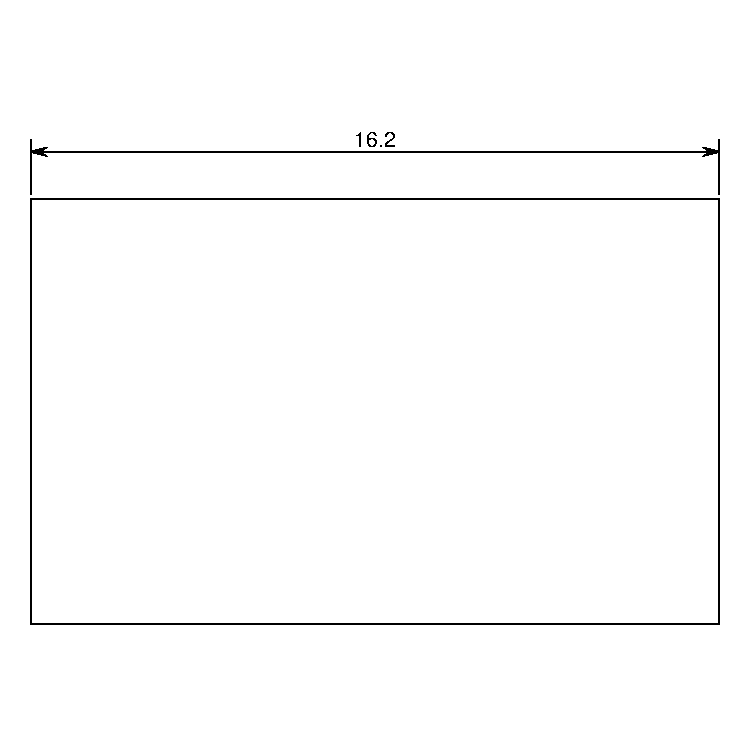
\includegraphics[width=3in,height=3in]{../images/example-horizontal-dimension.pdf}
\end{center}

\caption{HORIZONTAL-DIMENSION example}

\label{fig:HORIZONTAL-DIMENSION}

\end{figure}





\textbf{
\underline{Input slots (optional):}}

\begin{description}

\item [Base-plane-normal]
\index{Base-plane-normal
[horizontal-dimension]}

Must be specified in the subclass except for angular




\item [Dim-text-start]
\index{Dim-text-start
[horizontal-dimension]}\emph{3D Point}

 Determines where the text will start. Defaults to reasonable location for
horizontal-dimension.




\end{description}






\textbf{
\underline{Computed slots:}}

\begin{description}

\item [Leader-direction-1-vector]
\index{Leader-direction-1-vector
[horizontal-dimension]}

Must be specified in the subclass except for angular




\item [Leader-direction-2-vector]
\index{Leader-direction-2-vector
[horizontal-dimension]}

Must be specified in the subclass except for angular




\item [Witness-direction-vector]
\index{Witness-direction-vector
[horizontal-dimension]}

Must be specified in the subclass except for angular




\end{description}







\item \index{LABEL}
\label{prim:label}
\textbf{LABEL}


\textbf{
\underline{Mixins:}} OUTLINE-SPECIALIZATION-MIXIN, BASE-OBJECT





\begin{description}

\item [
\underline{Description}]


Produces a text label for graphical output



\end{description}




\begin{figure}
\begin{lrbox}{\boxedverb}
\begin{minipage}{\linewidth}
{\small

\begin{verbatim}        

 (in-package :gdl-user)
                   
 (define-object  label-sample (base-object)
  
   :objects
   ((box :type 'box
         :length 10 :width (* (the-child length) +phi+)
         :height (* (the-child :width) +phi+))
   
    (corner-label :type 'label
                  :leader-path (let ((start (the box (vertex :top :right :rear))))
                                (list start
                                      (translate start :right (/ (the box width) 10)
                                                       :rear (/ (the box width) 10))
                                      (translate start :right (/ (the box width) 7)
                                                       :rear (/ (the box width) 10))))
                  :text "The Corner"
                  :character-size (/ (the box width) 15))))


 (generate-sample-drawing :object-roots (make-object 'label-sample))


\end{verbatim}}
\end{minipage}
\end{lrbox}
\fbox{\usebox{\boxedverb}}

\caption{Example Code for LABEL}

\label{fig:example-code-LABEL}

\end{figure}

\begin{figure}
\begin{center}
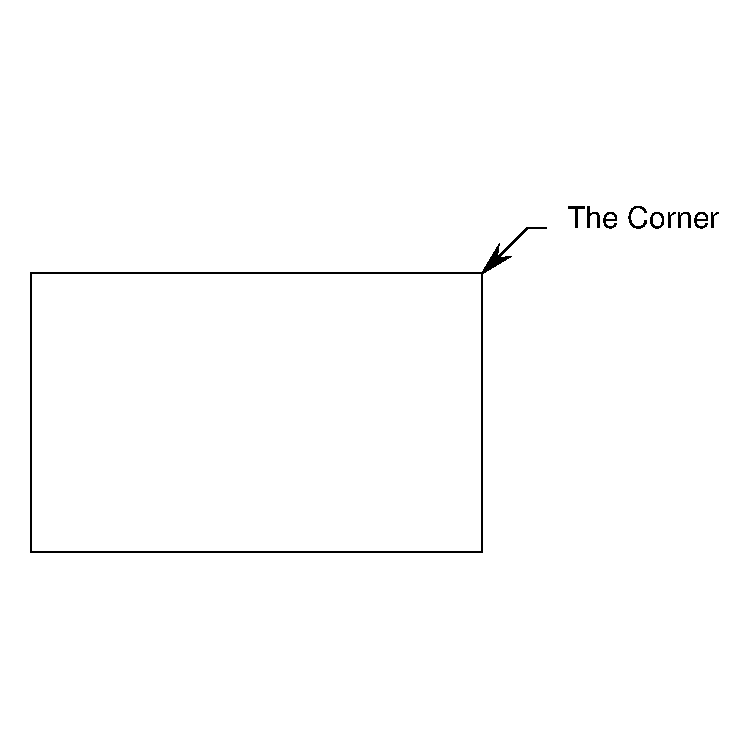
\includegraphics[width=3in,height=3in]{../images/example-label.pdf}
\end{center}

\caption{LABEL example}

\label{fig:LABEL}

\end{figure}





\textbf{
\underline{Input slots (required):}}

\begin{description}

\item [Leader-path]
\index{Leader-path
[label]}\emph{List of 3D Points}

 List making up leader line, starting from where the arrowhead normally is.




\end{description}






\textbf{
\underline{Input slots (optional):}}

\begin{description}

\item [Arrowhead-length]
\index{Arrowhead-length
[label]}\emph{Length (from tip to tail) of arrowhead glyph}

 Defaults to twice the \texttt{arrowhead-width}




\item [Arrowhead-style]
\index{Arrowhead-style
[label]}\emph{Keyword Symbol}

 Style for arrowhead at start of \texttt{leader-path}. Currently supported values
are \texttt{:none}, \texttt{:wedge}  (the Default), and \texttt{:double-wedge}.




\item [Arrowhead-style-2]
\index{Arrowhead-style-2
[label]}\emph{Keyword Symbol}

 Style for arrowhead on end of \texttt{leader-path}. Currently supported values
are \texttt{:none} (the Default), \texttt{:wedge}, and \texttt{:double-wedge}.




\item [Arrowhead-width]
\index{Arrowhead-width
[label]}\emph{Width of arrowhead glyph}

 Defaults to five times the line thickness (2.5)




\item [Character-size]
\index{Character-size
[label]}\emph{Number}

 Size (glyph height) of the label text, in model units. Defaults to 10.




\item [Dxf-font]
\index{Dxf-font
[label]}\emph{String}

 This names the DXF font for this general-note. Defaults to \texttt{(the font)}.




\item [Dxf-offset]
\index{Dxf-offset
[label]}\emph{Number}

 The start of text will be offset by this amount for DXF output. Default is 2.




\item [Dxf-size-ratio]
\index{Dxf-size-ratio
[label]}\emph{Number}

 The scale factor for DXF character size vs PDF character size. Default is 0.8




\item [Dxf-text-x-scale]
\index{Dxf-text-x-scale
[label]}\emph{Number in Percentage}

 Adjusts the character width for DXF output. Defaults to the text-x-scale.




\item [Font]
\index{Font
[label]}\emph{String naming a standard PDF font}

 Font for the label text. Defaults to "Helvetica"




\item [Outline-shape-type]
\index{Outline-shape-type
[label]}\emph{Keyword Symbol}

 Indicates shape of outline enclosing the text. Currently \texttt{:none}, \texttt{:bubble}, \texttt{:rectangle},
and \texttt{nil} are supported. The default is nil




\item [Strings]
\index{Strings
[label]}\emph{List of strings}

 Text lines to be displayed as the label. Specify this or text, not both.




\item [Text]
\index{Text
[label]}\emph{String}

 Text to be displayed as the label




\item [Text-gap]
\index{Text-gap
[label]}\emph{Number}

 Amount of space between last point in leader-path and beginning of the label text. Defaults to the
width of the letter "A" in the specified \texttt{font} and \texttt{character-size}.




\item [Text-side]
\index{Text-side
[label]}\emph{Keyword Symbol, either \texttt{:left} or \texttt{:right}}

 Determines whether the label text sits to
the right or the left of the last point in the \texttt{leader-path}. The default is computed based on
the direction of the last segment of the leader-path.




\item [View-reference-object]
\index{View-reference-object
[label]}\emph{GDL object or NIL}

 View object which will use this dimension. Defaults to NIL.




\end{description}






\textbf{
\underline{Computed slots:}}

\begin{description}

\item [Orientation]
\index{Orientation
[label]}\emph{3x3 Matrix of Double-Float Numbers}

 Indicates the absolute Rotation Matrix used to create
the coordinate system of this object. This matrix is given in absolute terms (i.e. with
respect to the root's orientation), and is generally created with the alignment function.
It should be an 
\i{orthonormal} matrix, meaning each row is a vector with a magnitude
of one (1.0).




\end{description}







\item \index{LEADER-LINE}
\label{prim:leader-line}
\textbf{LEADER-LINE}


\textbf{
\underline{Mixins:}} BASE-OBJECT





\begin{description}

\item [
\underline{Description}]


Creates a leader line with arrows on zero, one, or both ends



\end{description}








\textbf{
\underline{Input slots (required):}}

\begin{description}

\item [Path-points]
\index{Path-points
[leader-line]}\emph{List of 3D Points}

 Leader-line is rendered as a polyline going through these points.




\end{description}






\textbf{
\underline{Input slots (optional):}}

\begin{description}

\item [Arrowhead-length]
\index{Arrowhead-length
[leader-line]}\emph{Number}

 The length of the arrows. Defaults to (* (the arrowhead-width) 2)




\item [Arrowhead-style]
\index{Arrowhead-style
[leader-line]}\emph{Keyword}

 Controls the style of first arrowhead. Currently only :wedge is supported. Default is :wedge.




\item [Arrowhead-style-2]
\index{Arrowhead-style-2
[leader-line]}\emph{Keyword}

 Controls the style and presence of second arrowhead.
Currently only :wedge is supported. Default is :none.




\item [Arrowhead-width]
\index{Arrowhead-width
[leader-line]}\emph{Number}

 The width of the arrows. Defaults to (* (the line-thickness) 5).




\item [Break-points]
\index{Break-points
[leader-line]}\emph{List of two points or nil}

.
The start and end of the break in the leader line to accomodate the dimension-text,
in cases where there is overlap.




\end{description}






\textbf{
\underline{Computed slots:}}

\begin{description}

\item [Display-controls]
\index{Display-controls
[leader-line]}\emph{Plist}

 May contain keywords and values indicating display characteristics for
this object. The following keywords are recognized currently:



\begin{description}


\item[:color]
 color keyword from the *color-table* parameter, or an HTML-style hexidecimal
RGB string value, e.g. "\#FFFFFF" for pure white. Defaults to :black.


\item[:line-thickness]
 an integer, defaulting to 1, indicating relative line thickness for wireframe
representations of this object.


\item[:dash-pattern]
(currently PDF/PNG/JPEG only). This is a list of two or three numbers which indicate the length,
in pixels, of the dashes and blank spaces in a dashed line. The optional third number
indicates how far into the line or curve to start the dash pattern.

\end{description}





\end{description}







\item \index{LINE}
\label{prim:line}
\textbf{LINE}


\textbf{
\underline{Mixins:}} BASE-OBJECT





\begin{description}

\item [
\underline{Description}]


Provides a simple way to create a line, 
by specifying a start point and an end point.



\end{description}




\begin{figure}
\begin{lrbox}{\boxedverb}
\begin{minipage}{\linewidth}
{\small

\begin{verbatim}

  (in-package :gdl-user)  
  
  (define-object line-sample (line)
    :computed-slots
    ((start (make-point -10 -10 0))
     (end (make-point 10 10 0))))

  (generate-sample-drawing :objects (make-object 'line-sample))
  

\end{verbatim}}
\end{minipage}
\end{lrbox}
\fbox{\usebox{\boxedverb}}

\caption{Example Code for LINE}

\label{fig:example-code-LINE}

\end{figure}

\begin{figure}
\begin{center}

\includegraphics[width=3in,height=3in]{../images/example-line.pdf}
\end{center}

\caption{LINE example}

\label{fig:LINE}

\end{figure}





\textbf{
\underline{Input slots (required):}}

\begin{description}

\item [End]
\index{End
[line]}\emph{3D Point}

 The end point of the line, in global coordinates.




\item [Start]
\index{Start
[line]}\emph{3D Point}

 The start point of the line, in global coordinates.




\end{description}






\textbf{
\underline{Computed slots:}}

\begin{description}

\item [Bounding-box]
\index{Bounding-box
[line]}\emph{List of two 3D points}

 The left front bottom and right rear top corners, in global coordinates,
of the rectangular volume bounding the tree of geometric objects rooted at this object.




\item [Center]
\index{Center
[line]}\emph{3D Point}

 The center of the line.




\item [Direction-vector]
\index{Direction-vector
[line]}\emph{3D Vector}

 Points from start to end of the line.




\item [Length]
\index{Length
[line]}\emph{Number}

 The distance from start to end of the line.




\end{description}







\item \index{LINEAR-DIMENSION}
\label{prim:linear-dimension}
\textbf{LINEAR-DIMENSION}


\textbf{
\underline{Mixins:}} OUTLINE-SPECIALIZATION-MIXIN, BASE-OBJECT





\begin{description}

\item [
\underline{Description}]


Creates a dimension along either the
horizontal, vertical, or an arbitray axis. Use
\texttt{horizontal-dimension}, \texttt{vertical-dimension}, or
\texttt{parallel-dimension}, respectively, to achieve these.



\end{description}








\textbf{
\underline{Input slots (required):}}

\begin{description}

\item [Base-plane-normal]
\index{Base-plane-normal
[linear-dimension]}

Must be specified in the subclass except for angular




\item [End-point]
\index{End-point
[linear-dimension]}\emph{3D Point}

 Actual point where the dimension will stop measuring




\item [Leader-direction-1-vector]
\index{Leader-direction-1-vector
[linear-dimension]}

Must be specified in the subclass except for angular




\item [Leader-direction-2-vector]
\index{Leader-direction-2-vector
[linear-dimension]}

Must be specified in the subclass except for angular




\item [Start-point]
\index{Start-point
[linear-dimension]}\emph{3D Point}

 Actual point where the dimension will start measuring




\item [Witness-direction-vector]
\index{Witness-direction-vector
[linear-dimension]}

Must be specified in the subclass except for angular




\end{description}






\textbf{
\underline{Input slots (optional):}}

\begin{description}

\item [Arrowhead-length]
\index{Arrowhead-length
[linear-dimension]}\emph{Length (from tip to tail) of arrowhead glyph}

 Defaults to twice the \texttt{arrowhead-width}




\item [Arrowhead-style]
\index{Arrowhead-style
[linear-dimension]}\emph{Keyword Symbol}

 Style for arrowhead on end of \texttt{leader-line}. Currently supported values
are \texttt{:none}, \texttt{:wedge}  (the Default), and \texttt{:double-wedge}.




\item [Arrowhead-style-2]
\index{Arrowhead-style-2
[linear-dimension]}\emph{Keyword Symbol}

 Style for arrowhead on end of \texttt{leader-line}. Currently supported values
are \texttt{:none} (the Default), \texttt{:wedge}, and \texttt{:double-wedge}.




\item [Arrowhead-width]
\index{Arrowhead-width
[linear-dimension]}\emph{Width of arrowhead glyph}

 Defaults to half the character-size.




\item [Character-size]
\index{Character-size
[linear-dimension]}\emph{Number}

 Size (glyph height) of the label text, in model units. Defaults to 1.




\item [Dim-text]
\index{Dim-text
[linear-dimension]}\emph{String}

 Determines the text which shows up as the dimension label. Defaults to the dim-value,
which is computed specially in each specific dimension type.




\item [Dim-text-bias]
\index{Dim-text-bias
[linear-dimension]}\emph{Keyword symbol, :start, :end, or :center}

 Indicates where to position the text in the case when

\b{outside-leaders?} is non-nil. Defaults to :center




\item [Dim-text-start]
\index{Dim-text-start
[linear-dimension]}\emph{3D Point}

 Determines where the text will start. Defaults to halfway between start-point
and end-point.




\item [Dim-text-start-offset]
\index{Dim-text-start-offset
[linear-dimension]}\emph{3D Vector (normally only 2D are used)}

.
The dim-text-start is offset by this vector, in model space. Defaults to \#(0.0 0.0 0.0)




\item [Dim-value]
\index{Dim-value
[linear-dimension]}\emph{Number}

 2D distance relative to the base-plane-normal. Can be over-ridden in the subclass




\item [Dxf-font]
\index{Dxf-font
[linear-dimension]}\emph{String}

 This names the DXF font for this general-note. Defaults to \texttt{(the font)}.




\item [Dxf-offset]
\index{Dxf-offset
[linear-dimension]}\emph{Number}

 The start of text will be offset by this amount for DXF output. Default is 2.




\item [Dxf-size-ratio]
\index{Dxf-size-ratio
[linear-dimension]}\emph{Number}

 The scale factor for DXF character size vs PDF character size. Default is 0.8




\item [Dxf-text-x-scale]
\index{Dxf-text-x-scale
[linear-dimension]}\emph{Number in Percentage}

 Adjusts the character width for DXF output. Defaults to the text-x-scale.




\item [Flip-leaders?]
\index{Flip-leaders?
[linear-dimension]}\emph{Boolean}

 Indicates which direction the witness lines should take from the start and end points. The Default is NIL,
which indicates :rear (i.e. ``up'') for \texttt{horizontal-dimensions} and :right for \texttt{vertical-dimensions}




\item [Font]
\index{Font
[linear-dimension]}\emph{String naming a standard PDF font}

 Font for the label text. Defaults to "Helvetica"




\item [Full-leader-line-length]
\index{Full-leader-line-length
[linear-dimension]}\emph{Number}

 Indicates the length of the full leader when \texttt{outside-leaders?} is nil. This defaults to nil,
which indicates that the full-leader's length should be auto-computed based on the given start-point and end-point.




\item [Justification]
\index{Justification
[linear-dimension]}\emph{Keyword symbol, :left, :right, or :center}

.
For multi-line dim-text, this justification is applied.




\item [Leader-1?]
\index{Leader-1?
[linear-dimension]}\emph{Boolean}

 Indicates whether the first (or only) leader line should be displayed. The Default is T




\item [Leader-2?]
\index{Leader-2?
[linear-dimension]}\emph{Boolean}

 Indicates whether the second leader line should be displayed. The Default is T




\item [Leader-line-length]
\index{Leader-line-length
[linear-dimension]}\emph{Number}

 Indicates the length of the first leader for the case when \texttt{outside-leaders?} is non-NIL




\item [Leader-line-length-2]
\index{Leader-line-length-2
[linear-dimension]}\emph{Number}

 Indicates the length of the second leader for the case when \texttt{outside-leaders?} is non-NIL




\item [Leader-text-gap]
\index{Leader-text-gap
[linear-dimension]}\emph{Number}

 Amount of gap between leader lines and dimension text, when the dimension text is within the leader.
Defaults to half the character-size.




\item [Orientation]
\index{Orientation
[linear-dimension]}\emph{3x3 Matrix of Double-Float Numbers}

 Indicates the absolute Rotation Matrix used to create
the coordinate system of this object. This matrix is given in absolute terms (i.e. with
respect to the root's orientation), and is generally created with the alignment function.
It should be an 
\i{orthonormal} matrix, meaning each row is a vector with a magnitude
of one (1.0).




\item [Outline-shape-type]
\index{Outline-shape-type
[linear-dimension]}\emph{Keyword symbol}

 Currently can be :bubble, :rectangle, or :none. Default is :none.




\item [Outside-leaders-length-factor]
\index{Outside-leaders-length-factor
[linear-dimension]}\emph{Number}

 Indicates the default length of the outside-leaders as a multiple of arrowhead-length.
Defaults to 3.




\item [Outside-leaders?]
\index{Outside-leaders?
[linear-dimension]}\emph{Boolean}

 Indicates whether the leader line(s) should be inside or outside the interval between the start and
end points. The default is NIL, which indicates that the leader line(s) should be inside the interval




\item [Text-above-leader?]
\index{Text-above-leader?
[linear-dimension]}\emph{Boolean}

 Indicates whether the text is to the right or above the leader line, rather than in-line with it. Default is T.




\item [Text-along-axis?]
\index{Text-along-axis?
[linear-dimension]}\emph{Boolean}

 Where applicable, determines whether text direction follows leader-line direction




\item [Text-x-scale]
\index{Text-x-scale
[linear-dimension]}\emph{Number in Percentage}

 Adjusts the character width for the dimension-text and currently only applies only to PDF output




\item [Underline?]
\index{Underline?
[linear-dimension]}

GDL




\item [View-reference-object]
\index{View-reference-object
[linear-dimension]}\emph{GDL object or NIL}

 View object which will use this dimension. Defaults to NIL.




\item [Witness-line-2?]
\index{Witness-line-2?
[linear-dimension]}\emph{Boolean}

 Indicates whether to display a witness line coming off the \texttt{end-point}. Default is T




\item [Witness-line-ext]
\index{Witness-line-ext
[linear-dimension]}\emph{Number}

 Distance the witness line(s) extend beyond the leader line. Default is 0.3




\item [Witness-line-gap]
\index{Witness-line-gap
[linear-dimension]}\emph{Number}

 Distance from the \texttt{start-point} and \texttt{end-point} to the start of each witness-line. Default is 0.1




\item [Witness-line-length]
\index{Witness-line-length
[linear-dimension]}\emph{Number}

 Length of the witness lines (or of the shorter witness line in case they are different lengths)




\item [Witness-line?]
\index{Witness-line?
[linear-dimension]}\emph{Boolean}

 Indicates whether to display a witness line coming off the \texttt{start-point}. Default is T




\end{description}







\item \index{PARALLEL-DIMENSION}
\label{prim:parallel-dimension}
\textbf{PARALLEL-DIMENSION}


\textbf{
\underline{Mixins:}} LINEAR-DIMENSION





\begin{description}

\item [
\underline{Description}]


Creates a dimension annotation along an axis from a start point to an end point.



\end{description}




\begin{figure}
\begin{lrbox}{\boxedverb}
\begin{minipage}{\linewidth}
{\small

\begin{verbatim}        

 (in-package :gdl-user)
                   
 (define-object  parallel-dimension-sample (base-object)
  
  
   :objects
   ((box :type 'box
         :length 10 :width (* (the-child length) +phi+)
         :height (* (the-child :width) +phi+))
   
    (length-dimension :type 'parallel-dimension
                      :character-size (/ (the box length) 20)
                      :start-point (the box (vertex :top :left :front))
                      :end-point (the box (vertex :top :right :rear)))))

  (generate-sample-drawing :object-roots (make-object 'parallel-dimension-sample))


\end{verbatim}}
\end{minipage}
\end{lrbox}
\fbox{\usebox{\boxedverb}}

\caption{Example Code for PARALLEL-DIMENSION}

\label{fig:example-code-PARALLEL-DIMENSION}

\end{figure}

\begin{figure}
\begin{center}
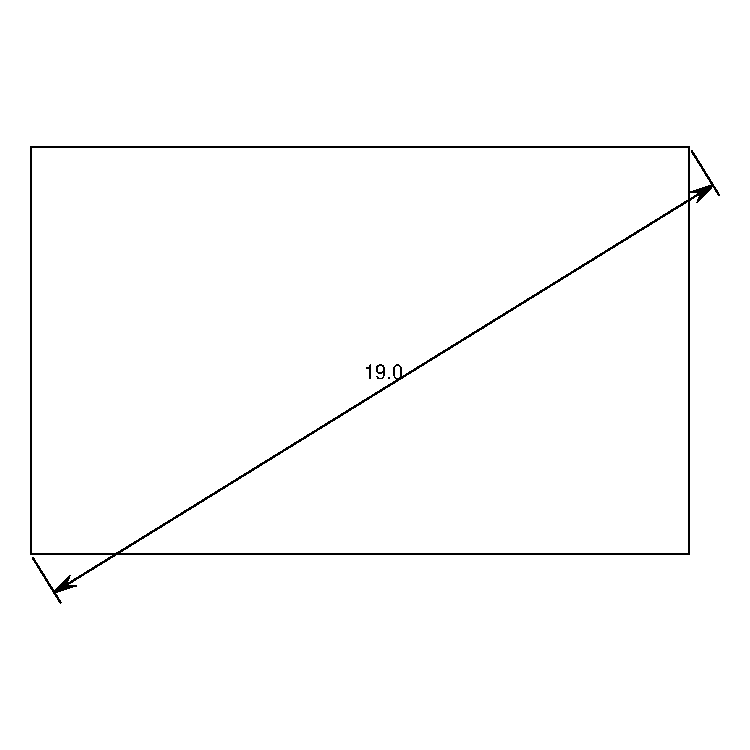
\includegraphics[width=3in,height=3in]{../images/example-parallel-dimension.pdf}
\end{center}

\caption{PARALLEL-DIMENSION example}

\label{fig:PARALLEL-DIMENSION}

\end{figure}





\textbf{
\underline{Input slots (optional):}}

\begin{description}

\item [Dim-text-start]
\index{Dim-text-start
[parallel-dimension]}\emph{3D Point}

 Determines where the text will start. Defaults to reasonable location for
horizontal-dimension.




\end{description}






\textbf{
\underline{Computed slots:}}

\begin{description}

\item [Base-plane-normal]
\index{Base-plane-normal
[parallel-dimension]}

Must be specified in the subclass except for angular




\item [Leader-direction-1-vector]
\index{Leader-direction-1-vector
[parallel-dimension]}

Must be specified in the subclass except for angular




\item [Leader-direction-2-vector]
\index{Leader-direction-2-vector
[parallel-dimension]}

Must be specified in the subclass except for angular




\item [Witness-direction-vector]
\index{Witness-direction-vector
[parallel-dimension]}

Must be specified in the subclass except for angular




\end{description}







\item \index{PIE-CHART}
\label{prim:pie-chart}
\textbf{PIE-CHART}


\textbf{
\underline{Mixins:}} BASE-OBJECT





\begin{description}

\item [
\underline{Description}]


Generates a standard Pie Chart with colored filled pie sections.

This object was inspired by the pie-chart in Marc Battyani's (marc.battyani(at)fractalconcept.com)
cl-pdf, with contributions from Carlos Ungil (Carlos.Ungil(at)cern.ch).



\end{description}




\begin{figure}
\begin{lrbox}{\boxedverb}
\begin{minipage}{\linewidth}
{\small

\begin{verbatim}

 (in-package :gdl-user)
 
 (define-object pie-sample (pie-chart)
   :computed-slots
   ((data (list 30 70))
   
    (labels&colors '(("Expenses" :red) ("Revenue" :green)))
   
    (width 200) 
   
    (title "Cash Flow")))

 (generate-sample-drawing :objects (make-object 'pie-sample))

 
\end{verbatim}}
\end{minipage}
\end{lrbox}
\fbox{\usebox{\boxedverb}}

\caption{Example Code for PIE-CHART}

\label{fig:example-code-PIE-CHART}

\end{figure}

\begin{figure}
\begin{center}
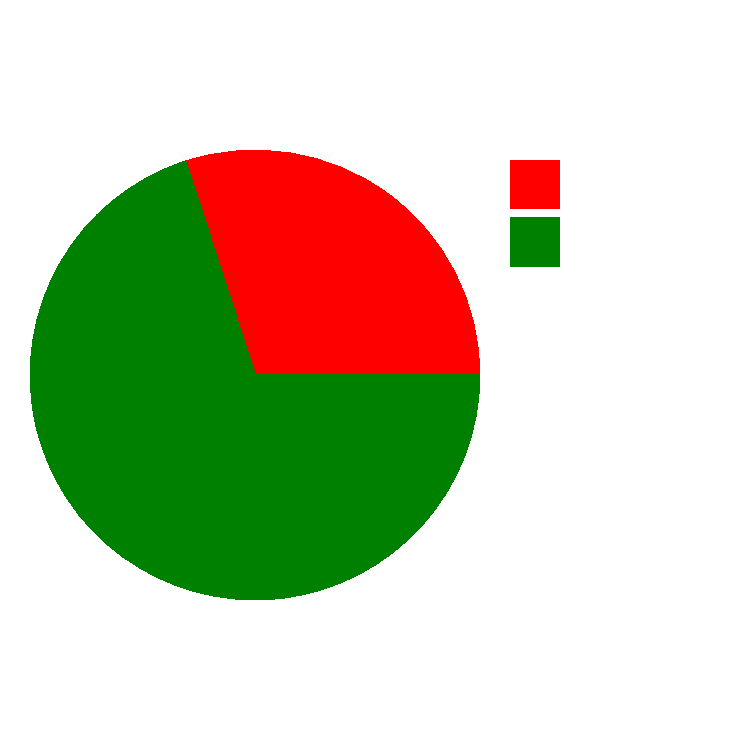
\includegraphics[width=3in,height=3in]{../images/example-pie-chart.pdf}
\end{center}

\caption{PIE-CHART example}

\label{fig:PIE-CHART}

\end{figure}





\textbf{
\underline{Input slots (optional):}}

\begin{description}

\item [Data]
\index{Data
[pie-chart]}\emph{List of Numbers}

 The relative size for each pie piece. These will be normalized to percentages.
Defaults to NIL, must be specified as non-NIL to get a result.




\item [Include-legend?]
\index{Include-legend?
[pie-chart]}\emph{Boolean}

 Determines whether the Legend is included in standard output formats. Defaults to \texttt{t}.




\item [Labels\&colors]
\index{Labels\&colors
[pie-chart]}\emph{List of lists, each containing a string and a keyword symbol}

 This list should be the same
length as \texttt{data}. These colors and labels will be assigned to each pie piece and to the legend.
Defaults to NIL, must be specified as non-NIL to get a result.




\item [Line-color]
\index{Line-color
[pie-chart]}\emph{Keyword symbol naming color from \texttt{*color-table*}}

.
Color of the outline of the pie. Defaults to :black.




\item [Radius]
\index{Radius
[pie-chart]}\emph{Number}

 The radius of the pie. Defaults to 0.35 times the \texttt{width}.




\item [Title]
\index{Title
[pie-chart]}\emph{String}

 Title for the chart. Defaults to the empty string.




\item [Title-color]
\index{Title-color
[pie-chart]}\emph{Keyword symbol naming color from \texttt{*color-table*}}

.
Color of title text. Defaults to :black.




\item [Title-font]
\index{Title-font
[pie-chart]}\emph{String}

 Currently this must be a PDF font name. Defaults to "Helvetica."




\item [Title-font-size]
\index{Title-font-size
[pie-chart]}\emph{Number}

 Size in points of title font. Defaults to 12.




\end{description}







\item \index{POINT}
\label{prim:point}
\textbf{POINT}


\textbf{
\underline{Mixins:}} SPHERE





\begin{description}

\item [
\underline{Description}]


Visual representation of a point as a small view-independent crosshair. This means
the crosshair will always appear in a ``top'' view regardless of the current view transform. The crosshair will
not scale along with any zoom state unless the \texttt{scale?} optional input-slot is non-NIL. The default
color for the crosshairs is a light grey (:grey-light-very in the *color-table*).



\end{description}




\begin{figure}
\begin{lrbox}{\boxedverb}
\begin{minipage}{\linewidth}
{\small

\begin{verbatim}

 (in-package :gdl-user)

 (define-object point-sample (base-object)
   
   :objects
   ((bezier :type 'bezier-curve
            :control-points (list (make-point 0 0 0)
                                  (make-point 1 1 0)
                                  (make-point 2 1 0)
                                  (make-point 3 0 0)))
    (points-to-show :type 'point
                    :sequence (:size (length (the bezier control-points)))
                    :center (nth (the-child :index) 
                                 (the bezier control-points))
                    :radius 0.08
                    :display-controls (list :color :blue))))

 (generate-sample-drawing :object-roots (make-object 'point-sample))


\end{verbatim}}
\end{minipage}
\end{lrbox}
\fbox{\usebox{\boxedverb}}

\caption{Example Code for POINT}

\label{fig:example-code-POINT}

\end{figure}

\begin{figure}
\begin{center}
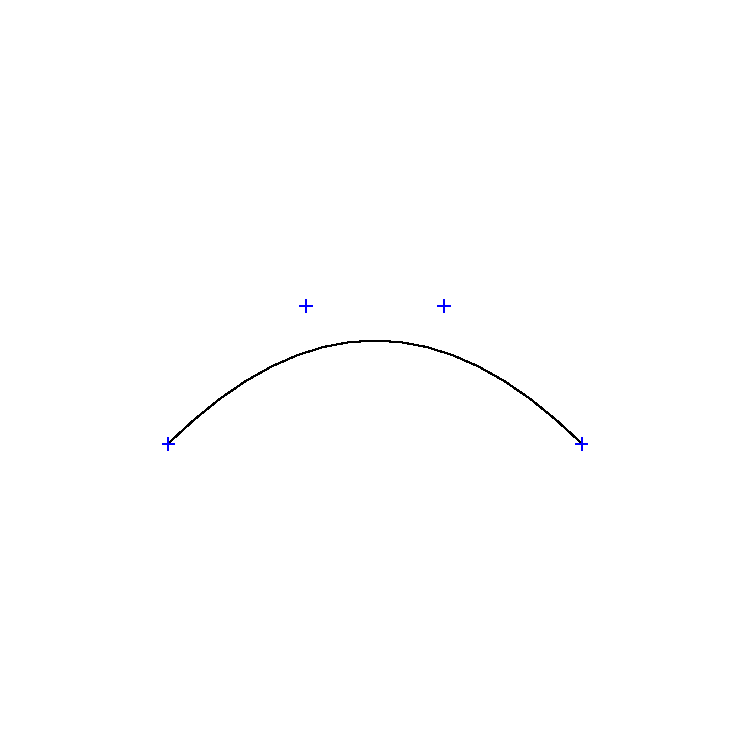
\includegraphics[width=3in,height=3in]{../images/example-point.pdf}
\end{center}

\caption{POINT example}

\label{fig:POINT}

\end{figure}





\textbf{
\underline{Input slots (optional):}}

\begin{description}

\item [Crosshair-length]
\index{Crosshair-length
[point]}\emph{Number}

 Distance from center to end of crosshairs used to show the point. Default value is 3.




\item [Radius]
\index{Radius
[point]}\emph{Number}

 Distance from center to any point on the sphere.




\item [Scaled?]
\index{Scaled?
[point]}\emph{Boolean}

 Indicates whether the crosshairs drawn to represent the point are scaled along with
any zoom factor applied to the display, or are fixed with respect to drawing space. The default is NIL,
meaning the crosshairs will remain the same size regardless of zoom state.




\end{description}






\textbf{
\underline{Computed slots:}}

\begin{description}

\item [Bounding-box]
\index{Bounding-box
[point]}\emph{List of two 3D points}

 The left front bottom and right rear top corners, in global coordinates,
of the rectangular volume bounding the tree of geometric objects rooted at this object.




\end{description}







\item \index{POINTS-DISPLAY}
\label{prim:points-display}
\textbf{POINTS-DISPLAY}


\textbf{
\underline{Mixins:}} OUTLINE-SPECIALIZATION-MIXIN





\begin{description}

\item [
\underline{Description}]


Product a list of hidden-children which are GDL point objects, which 
will be displayed in normal renderings using the \texttt{outline-specialization-mixin} mechanism.



\end{description}








\textbf{
\underline{Input slots (required):}}

\begin{description}

\item [Points]
\index{Points
[points-display]}\emph{List of 3D points (i}

e. vectors). The points to be displayed.




\end{description}







\item \index{RENDERER-MIXIN}
\label{prim:renderer-mixin}
\textbf{RENDERER-MIXIN}


\textbf{
\underline{Mixins:}} VANILLA-MIXIN





\begin{description}

\item [
\underline{Description}]


Object mixed into the base-view to compute required values to provide
a rendered perspective view, as in VRML.



\end{description}








\textbf{
\underline{Input slots (required):}}

\begin{description}

\item [Object-roots]
\index{Object-roots
[renderer-mixin]}\emph{List of GDL Objects}

 Roots of the leaf objects to be displayed in this renderer view.




\item [Objects]
\index{Objects
[renderer-mixin]}\emph{List of GDL Objects}

 Leaves of the objects to be displayed in this renderer view.




\end{description}






\textbf{
\underline{Input slots (optional):}}

\begin{description}

\item [3D-box]
\index{3D-box
[renderer-mixin]}\emph{List of two 3D points}

 The left-front-lower and right-rear-upper corners of the axis-aligned bounding
box of the \texttt{object-roots} and \texttt{objects}.




\item [3D-box-center]
\index{3D-box-center
[renderer-mixin]}\emph{3D Point}

 The effective view center for the scene contained in this view object. Defaults to the center of the bounding sphere of all
the objects in the scene, consisting of the \texttt{object-roots} and the \texttt{objects}.




\item [Bounding-sphere]
\index{Bounding-sphere
[renderer-mixin]}\emph{Plist containing keys: \texttt{:center} and \texttt{:radius}}

 This plist represents the tightest-fitting sphere
around all the objects listed in the \texttt{object-roots} and the \texttt{objects}




\item [Field-of-view-default]
\index{Field-of-view-default
[renderer-mixin]}\emph{Number in angular degrees}

 The maximum angle of the view frustrum for perspective views.
Defaults to 0.1 (which results in a near parallel projection with virtually no perspective effect).




\item [View-vectors]
\index{View-vectors
[renderer-mixin]}\emph{Plist}

 Keys indicate view vector names (e.g. \texttt{:trimetric}), and values contain the 3D vectors. Defaults to the
parameter \texttt{*standard-views*}, but with the key corresponding to current \texttt{(the view)} ordered
first in the plist. This list of view-vectors is used to construct the default \texttt{viewpoints}.




\item [Viewpoints]
\index{Viewpoints
[renderer-mixin]}\emph{List of Plists}

 Each plist contains, based on each entry in the \texttt{view-vectors}, keys:


\begin{itemize}

\item \texttt{:point} (camera location, defaults to the \texttt{3d-box-center} translated
along the corresponding element of \texttt{view-vectors}) by the local camera distance.
The camera distance is computed based on the field-of-view angle and
the \texttt{bounding-sphere}


\item \texttt{:orientation} (3d matrix indicating camera orientation)


\item \texttt{field-of-view} Angle in degrees of the view frustrum (i.e. lens angle of the virtual camera).


\end{itemize}





\end{description}







\item \index{ROUTE-PIPE}
\label{prim:route-pipe}
\textbf{ROUTE-PIPE}


\textbf{
\underline{Mixins:}} GLOBAL-FILLETED-POLYLINE-MIXIN, OUTLINE-SPECIALIZATION-MIXIN





\begin{description}

\item [
\underline{Description}]


Defines an alternating set of cylinders and torus sections for the elbows



\end{description}




\begin{figure}
\begin{lrbox}{\boxedverb}
\begin{minipage}{\linewidth}
{\small

\begin{verbatim}

 (in-package :gdl-user)  

 (define-object route-pipe-sample (base-object)

  :objects

  ((pipe :type 'route-pipe
         :vertex-list (list #(410.36 436.12 664.68) 
                            #(404.21 436.12 734.97) 
                            #(402.22 397.48 757.72) 
                            #(407.24 397.48 801.12) 
                            #(407.24 448.0 837.0)
                            #(346.76 448.0 837.0))
         :default-radius 19
         :outer-pipe-radius 7
         :inner-pipe-radius nil
         :display-controls (list :color :blue-steel 
                                 :transparency 0.0 
                                 :shininess 0.7 
                                 :spectral-color :white))))

 
 (generate-sample-drawing :objects (the-object (make-object 'route-pipe-sample) pipe)
                          :projection-direction (getf *standard-views* :trimetric))
  



\end{verbatim}}
\end{minipage}
\end{lrbox}
\fbox{\usebox{\boxedverb}}

\caption{Example Code for ROUTE-PIPE}

\label{fig:example-code-ROUTE-PIPE}

\end{figure}

\begin{figure}
\begin{center}
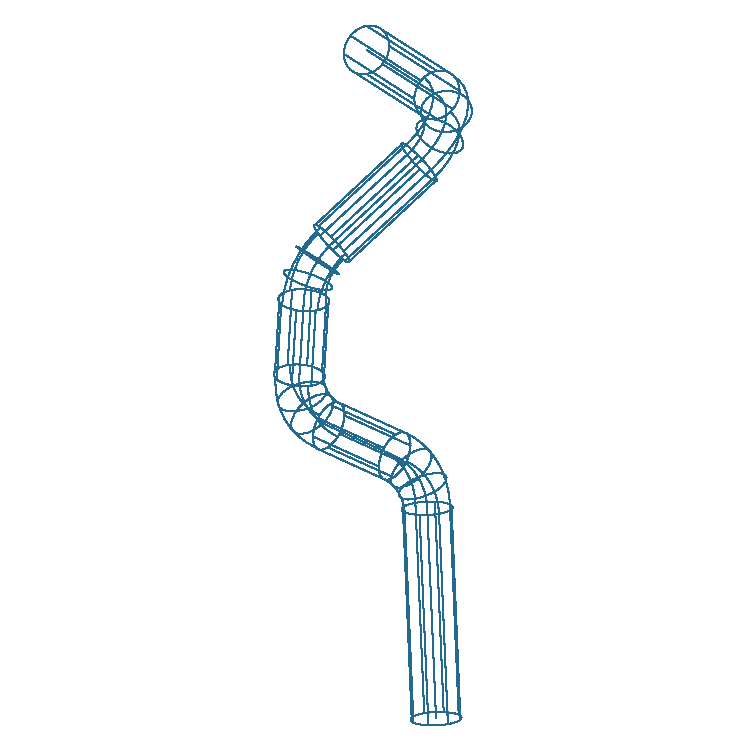
\includegraphics[width=3in,height=3in]{../images/example-route-pipe.pdf}
\end{center}

\caption{ROUTE-PIPE example}

\label{fig:ROUTE-PIPE}

\end{figure}





\textbf{
\underline{Input slots (required):}}

\begin{description}

\item [Outer-pipe-radius]
\index{Outer-pipe-radius
[route-pipe]}\emph{Number}

 Radius to the outer surface of the piping.




\item [Vertex-list]
\index{Vertex-list
[route-pipe]}\emph{List of 3D Points}

 Same as for global-filleted-polyline (which is mixed in to this part)




\end{description}






\textbf{
\underline{Input slots (optional):}}

\begin{description}

\item [Inner-pipe-radius]
\index{Inner-pipe-radius
[route-pipe]}\emph{Number}

 Radius of the inner hollow part of the piping. NIL for a solid pipe.




\end{description}






\textbf{
\underline{Computed slots:}}

\begin{description}

\item [Bounding-box]
\index{Bounding-box
[route-pipe]}\emph{List of two 3D points}

 The left front bottom and right rear top corners, in global coordinates,
of the rectangular volume bounding the tree of geometric objects rooted at this object.




\item [Height]
\index{Height
[route-pipe]}\emph{Number}

 Z-axis dimension of the reference box. Defaults to zero.




\item [Length]
\index{Length
[route-pipe]}\emph{Number}

 Y-axis dimension of the reference box. Defaults to zero.




\item [Orientation]
\index{Orientation
[route-pipe]}\emph{3x3 Matrix of Double-Float Numbers}

 Indicates the absolute Rotation Matrix used to create
the coordinate system of this object. This matrix is given in absolute terms (i.e. with
respect to the root's orientation), and is generally created with the alignment function.
It should be an 
\i{orthonormal} matrix, meaning each row is a vector with a magnitude
of one (1.0).




\item [Width]
\index{Width
[route-pipe]}\emph{Number}

 X-axis dimension of the reference box. Defaults to zero.




\end{description}







\item \index{SAMPLE-DRAWING}
\label{prim:sample-drawing}
\textbf{SAMPLE-DRAWING}


\textbf{
\underline{Mixins:}} BASE-DRAWING, VANILLA-MIXIN





\begin{description}

\item [
\underline{Description}]


Defines a simple drawing with a single view for displaying objects or object-roots.



\end{description}








\textbf{
\underline{Input slots (optional):}}

\begin{description}

\item [Page-length]
\index{Page-length
[sample-drawing]}\emph{Number in PDF Points}

 Front-to-back (or top-to-bottom) length of the paper being represented
by this drawing. The default is (* 11 72) points, or 11 inches, corresponding to US standard
letter-size paper.




\item [Page-width]
\index{Page-width
[sample-drawing]}\emph{Number in PDF Points}

 Left-to-right width of the paper being represented by this drawing.
The default is (* 8.5 72) points, or 8.5 inches, corresponding to US standard letter-size paper.




\end{description}







\item \index{SPHERE}
\label{prim:sphere}
\textbf{SPHERE}


\textbf{
\underline{Mixins:}} IFS-OUTPUT-MIXIN, ARCOID-MIXIN, BASE-OBJECT





\begin{description}

\item [
\underline{Description}]


The set of points equidistant from a given center point.



\end{description}




\begin{figure}
\begin{lrbox}{\boxedverb}
\begin{minipage}{\linewidth}
{\small

\begin{verbatim}
  
  (in-package :gdl-user)
  
  (define-object sphere-sample (sphere)
    
   :computed-slots

    ((radius 150)
     (number-of-vertical-sections 10)
     (number-of-horizontal-sections 10)
     (display-controls (list :color :green-forest-medium))))

  (generate-sample-drawing :objects (make-object 'sphere-sample) 
                           :projection-direction :trimetric)





                  

\end{verbatim}}
\end{minipage}
\end{lrbox}
\fbox{\usebox{\boxedverb}}

\caption{Example Code for SPHERE}

\label{fig:example-code-SPHERE}

\end{figure}

\begin{figure}
\begin{center}

\includegraphics[width=3in,height=3in]{../images/example-sphere.pdf}
\end{center}

\caption{SPHERE example}

\label{fig:SPHERE}

\end{figure}





\textbf{
\underline{Input slots (required):}}

\begin{description}

\item [Radius]
\index{Radius
[sphere]}\emph{Number}

 Distance from center to any point on the sphere.




\end{description}






\textbf{
\underline{Input slots (optional):}}

\begin{description}

\item [End-horizontal-arc]
\index{End-horizontal-arc
[sphere]}\emph{Angle in radians}

 Ending horizontal angle for a partial sphere. Default is twice pi.




\item [End-vertical-arc]
\index{End-vertical-arc
[sphere]}\emph{Angle in radians}

 Ending vertical angle for a partial sphere. Default is pi/2.




\item [Inner-radius]
\index{Inner-radius
[sphere]}\emph{Number}

 Radius of inner hollow for a hollow sphere. Default is NIL, for a non-hollow sphere.




\item [Number-of-horizontal-sections]
\index{Number-of-horizontal-sections
[sphere]}\emph{Number}

 How many lines of latitude to show on the sphere in some renderings. Default value is 4.




\item [Number-of-vertical-sections]
\index{Number-of-vertical-sections
[sphere]}\emph{Number}

 How many lines of longitude to show on the sphere in some renderings. Default value is 4.




\item [Start-horizontal-arc]
\index{Start-horizontal-arc
[sphere]}\emph{Angle in radians}

 Starting horizontal angle for a partial sphere. Default is 0.




\item [Start-vertical-arc]
\index{Start-vertical-arc
[sphere]}\emph{Angle in radians}

 Starting vertical angle for a partial sphere. Default is -pi/2.




\end{description}






\textbf{
\underline{Computed slots:}}

\begin{description}

\item [Height]
\index{Height
[sphere]}\emph{Number}

 Z-axis dimension of the reference box. Defaults to zero.




\item [Length]
\index{Length
[sphere]}\emph{Number}

 Y-axis dimension of the reference box. Defaults to zero.




\item [Width]
\index{Width
[sphere]}\emph{Number}

 X-axis dimension of the reference box. Defaults to zero.




\end{description}







\item \index{SPHERICAL-CAP}
\label{prim:spherical-cap}
\textbf{SPHERICAL-CAP}


\textbf{
\underline{Mixins:}} IFS-OUTPUT-MIXIN, ARCOID-MIXIN, BASE-OBJECT





\begin{description}

\item [
\underline{Description}]


The region of a sphere which lies above (or below) a given plane. Although this
could be created with a partial sphere using the sphere primitive, the spherical cap allows for more convenient
construction and positioning since the actual center of the spherical cap is the center of its reference box.



\end{description}




\begin{figure}
\begin{lrbox}{\boxedverb}
\begin{minipage}{\linewidth}
{\small

\begin{verbatim}
  
 (in-package :gdl-user)

 (define-object spherical-cap-sample (spherical-cap)
   
  :computed-slots

   ((base-radius 150)
    (cap-thickness 7)
    (axis-length (* (the base-radius) +phi+))
    (number-of-vertical-sections 10)
    (number-of-horizontal-sections 10)
    (display-controls (list :color :orchid-medium :transparency 0.5))))
  

 (generate-sample-drawing :objects (make-object 'spherical-cap-sample) 
                          :projection-direction :trimetric)
                  

\end{verbatim}}
\end{minipage}
\end{lrbox}
\fbox{\usebox{\boxedverb}}

\caption{Example Code for SPHERICAL-CAP}

\label{fig:example-code-SPHERICAL-CAP}

\end{figure}

\begin{figure}
\begin{center}
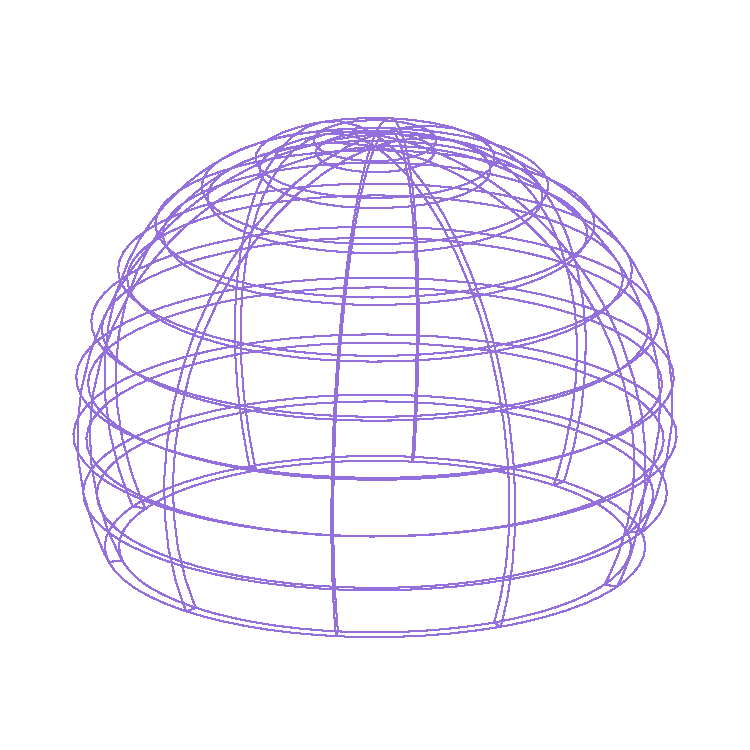
\includegraphics[width=3in,height=3in]{../images/example-spherical-cap.pdf}
\end{center}

\caption{SPHERICAL-CAP example}

\label{fig:SPHERICAL-CAP}

\end{figure}





\textbf{
\underline{Input slots (required):}}

\begin{description}

\item [Axis-length]
\index{Axis-length
[spherical-cap]}\emph{Number}

 The distance from the center of the base to the center of the dome.




\item [Base-radius]
\index{Base-radius
[spherical-cap]}\emph{Number}

 Radius of the base.




\end{description}






\textbf{
\underline{Input slots (optional):}}

\begin{description}

\item [Cap-thickness]
\index{Cap-thickness
[spherical-cap]}\emph{Number}

 Thickness of the shell for a hollow spherical-cap. Specify this
or inner-base-radius, not both.




\item [Inner-base-radius]
\index{Inner-base-radius
[spherical-cap]}\emph{Number}

 Radius of base of inner for a hollow spherical-cap. Specify this
or cap-thickness, not both.




\item [Number-of-horizontal-sections]
\index{Number-of-horizontal-sections
[spherical-cap]}\emph{Integer}

 How many lines of latitude to show on the spherical-cap in some renderings. Default value is 2.




\item [Number-of-vertical-sections]
\index{Number-of-vertical-sections
[spherical-cap]}\emph{Integer}

 How many lines of longitude to show on the spherical-cap in some renderings. Default value is 2.




\end{description}






\textbf{
\underline{Computed slots:}}

\begin{description}

\item [End-angle]
\index{End-angle
[spherical-cap]}\emph{Angle in radians}

 End angle of the arc. Defaults to twice pi.




\item [Height]
\index{Height
[spherical-cap]}\emph{Number}

 Z-axis dimension of the reference box. Defaults to zero.




\item [Length]
\index{Length
[spherical-cap]}\emph{Number}

 Y-axis dimension of the reference box. Defaults to zero.




\item [Sphere-center]
\index{Sphere-center
[spherical-cap]}\emph{3D Point}

 Center of the sphere containing the spherical-cap.




\item [Sphere-radius]
\index{Sphere-radius
[spherical-cap]}\emph{Number}

 Radius of the sphere containing the spherical-cap.




\item [Start-angle]
\index{Start-angle
[spherical-cap]}\emph{Angle in radians}

 Start angle of the arc. Defaults to zero.




\item [Width]
\index{Width
[spherical-cap]}\emph{Number}

 X-axis dimension of the reference box. Defaults to zero.




\end{description}







\item \index{TEXT-LINE}
\label{prim:text-line}
\textbf{TEXT-LINE}


\textbf{
\underline{Mixins:}} BASE-OBJECT





\begin{description}

\item [
\underline{Description}]


Outputs a single line of text for graphical display.



\end{description}








\textbf{
\underline{Input slots (optional):}}

\begin{description}

\item [Center]
\index{Center
[text-line]}\emph{3D-point}

 Center of the text. Specify this or start, not both.




\item [Start]
\index{Start
[text-line]}\emph{3D-point}

 Start of the text. Specify this or center, not both.




\item [Width]
\index{Width
[text-line]}\emph{Number}

 X-axis dimension of the reference box. Defaults to zero.




\end{description}






\textbf{
\underline{Computed slots:}}

\begin{description}

\item [Length]
\index{Length
[text-line]}\emph{Number}

 Y-axis dimension of the reference box. Defaults to zero.




\end{description}







\item \index{TORUS}
\label{prim:torus}
\textbf{TORUS}


\textbf{
\underline{Mixins:}} IFS-OUTPUT-MIXIN, ARCOID-MIXIN, BASE-OBJECT





\begin{description}

\item [
\underline{Description}]


A single-holed ``ring'' torus, also known as an ``anchor ring.''
This is basically a circular cylinder ``bent'' into a donut shape. Partial donuts (``elbows'') are supported.
Partial ``bent'' cylinders are not currently supported.



\end{description}




\begin{figure}
\begin{lrbox}{\boxedverb}
\begin{minipage}{\linewidth}
{\small

\begin{verbatim}
  
  (in-package :gdl-user)
  
  (define-object torus-sample (torus)
    :computed-slots
    ((major-radius 150)
     (minor-radius 42)
     (draw-centerline-arc? t)
     (number-of-longitudinal-sections 10)
     (number-of-transverse-sections 10)
     (display-controls (list :color :green-forest-medium)))

    :hidden-objects ((view :type 'base-view
                           :projection-vector (getf *standard-views* :trimetric)
                           :page-width (* 5 72) :page-length (* 5 72)
                           :objects (list self))))
  

  (generate-sample-drawing :objects (make-object 'torus-sample) 
                           :projection-direction :trimetric)
                  

\end{verbatim}}
\end{minipage}
\end{lrbox}
\fbox{\usebox{\boxedverb}}

\caption{Example Code for TORUS}

\label{fig:example-code-TORUS}

\end{figure}

\begin{figure}
\begin{center}
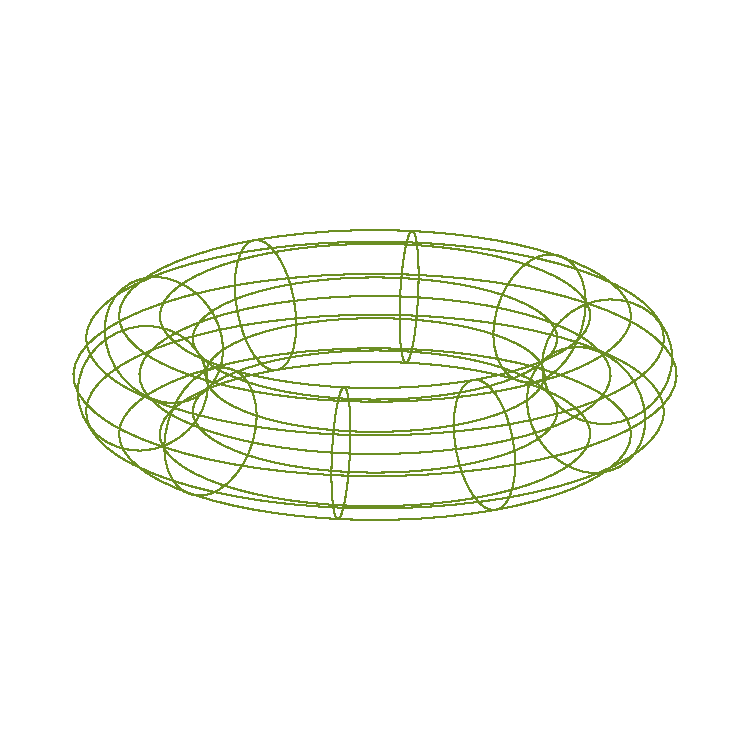
\includegraphics[width=3in,height=3in]{../images/example-torus.pdf}
\end{center}

\caption{TORUS example}

\label{fig:TORUS}

\end{figure}





\textbf{
\underline{Input slots (required):}}

\begin{description}

\item [Major-radius]
\index{Major-radius
[torus]}\emph{Number}

 Distance from center of donut hole to centerline of the torus.




\item [Minor-radius]
\index{Minor-radius
[torus]}\emph{Number}

 Radius of the bent cylinder making up the torus.




\end{description}






\textbf{
\underline{Input slots (optional):}}

\begin{description}

\item [Draw-centerline-arc?]
\index{Draw-centerline-arc?
[torus]}\emph{Boolean}

 Indicates whether the bent cylinder's centerline arc should be rendered in some renderings.




\item [End-caps?]
\index{End-caps?
[torus]}\emph{Boolean}

 Indicates whether to include end caps for a partial torus in some renderings. Defaults to T.




\item [Inner-minor-radius]
\index{Inner-minor-radius
[torus]}\emph{Number}

 Radius of the inner hollow part of the bent cylinder for a hollow torus. Defaults to NIL for a solid cylinder




\item [Number-of-longitudinal-sections]
\index{Number-of-longitudinal-sections
[torus]}\emph{Integer}

 Indicates the number of arcs to be drawn on along ``surface'' of the torus in some wireframe renderings.




\item [Number-of-transverse-sections]
\index{Number-of-transverse-sections
[torus]}\emph{Integer}

 Indicates the number of circular cross-sections of the bent cylinder to show in some wireframe renderings.




\end{description}






\textbf{
\underline{Input slots (optional, defaulting):}}

\begin{description}

\item [Arc]
\index{Arc
[torus]}\emph{Angle in Radians}

 Indicates the end angle for the donut. Defaults to twice pi for a full-circle donut.




\end{description}






\textbf{
\underline{Computed slots:}}

\begin{description}

\item [Height]
\index{Height
[torus]}\emph{Number}

 Z-axis dimension of the reference box. Defaults to zero.




\item [Length]
\index{Length
[torus]}\emph{Number}

 Y-axis dimension of the reference box. Defaults to zero.




\item [Width]
\index{Width
[torus]}\emph{Number}

 X-axis dimension of the reference box. Defaults to zero.




\end{description}







\item \index{TYPESET-BLOCK}
\label{prim:typeset-block}
\textbf{TYPESET-BLOCK}


\textbf{
\underline{Mixins:}} BASE-OBJECT





\begin{description}

\item [
\underline{Description}]


Block of text typeset using cl-typesetting. This object
wraps the typeset block as a standard GDL object, so it can be placed in a view and 
positioned according to normal GDL positioning.

You can specify the width, and by default this object will compute its length automatically 
from the typeset content, to fit all the lines of text into the box. Because of this 
computed behavior of the length, the center of the box will not, in general, be in a 
known location compared to the start of the text. Because of this it is recommended
to use :corner, rather than :center, for positioning a base-view which contains
a typeset block. 

In the normal case, if you want a single block in a view on a drawing, you should
make the base-view object have the same width and length as the typeset-block. The
base-view should also probably have :left-margin 0 and :front-margin 0.



\end{description}








\textbf{
\underline{Input slots (optional):}}

\begin{description}

\item [Center]
\index{Center
[typeset-block]}\emph{3D-point}

 Center of the text. Specify this or start, not both.




\item [Length]
\index{Length
[typeset-block]}\emph{Number}

 The length of the box to contain the compiled content. Defaults is (the length-default),
which will exactly fit the compiled content into the specified width. If you override it to be less
than this default, the content will be cropped.




\item [Start]
\index{Start
[typeset-block]}\emph{3D-point}

 Start of the text. Specify this or center, not both.




\item [Start-line-index]
\index{Start-line-index
[typeset-block]}\emph{Number}

 The line number to start




\end{description}






\textbf{
\underline{Computed slots:}}

\begin{description}

\item [Length-default]
\index{Length-default
[typeset-block]}\emph{Number}

 The computed length which will exactly fit the content based on (the width).




\item [Lines]
\index{Lines
[typeset-block]}\emph{List of typeset line objects}

 The list of lines in the nominal block.




\end{description}







\item \index{VERTICAL-DIMENSION}
\label{prim:vertical-dimension}
\textbf{VERTICAL-DIMENSION}


\textbf{
\underline{Mixins:}} LINEAR-DIMENSION





\begin{description}

\item [
\underline{Description}]


Creates a dimension annotation along the vertical axis.



\end{description}




\begin{figure}
\begin{lrbox}{\boxedverb}
\begin{minipage}{\linewidth}
{\small

\begin{verbatim}        

 (in-package :gdl-user)
                   
 (define-object  vertical-dimension-sample (base-object)
  
  
   :objects
   ((box :type 'box
         :length 10 :width (* (the-child length) +phi+)
         :height (* (the-child :width) +phi+))
   
    (length-dimension :type 'vertical-dimension
                      :character-size (/ (the box length) 20)
                      :flip-leaders? t
                      :start-point (the box (vertex :top :left :front))
                      :end-point (the box (vertex :top :left :rear)))))

 (generate-sample-drawing :object-roots (make-object 'vertical-dimension-sample))


\end{verbatim}}
\end{minipage}
\end{lrbox}
\fbox{\usebox{\boxedverb}}

\caption{Example Code for VERTICAL-DIMENSION}

\label{fig:example-code-VERTICAL-DIMENSION}

\end{figure}

\begin{figure}
\begin{center}
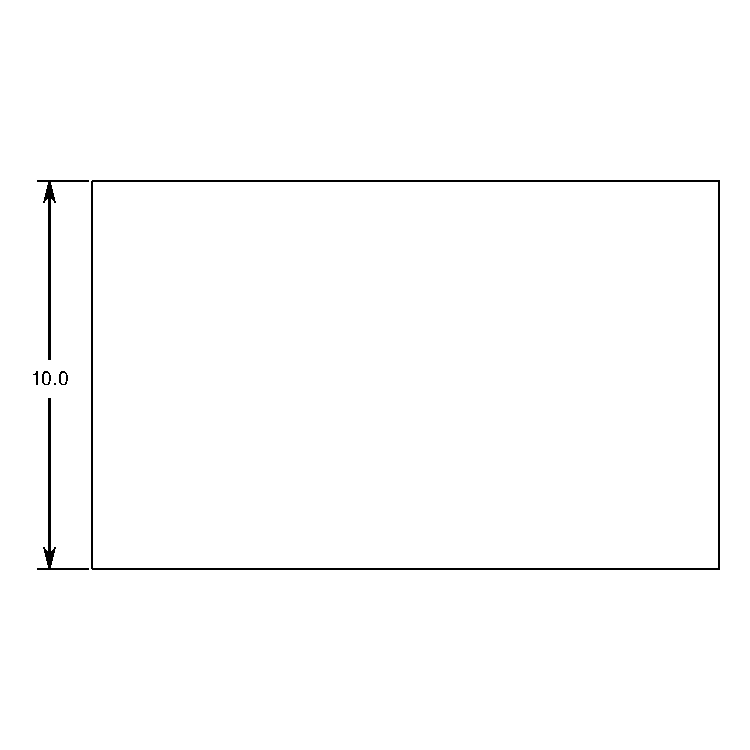
\includegraphics[width=3in,height=3in]{../images/example-vertical-dimension.pdf}
\end{center}

\caption{VERTICAL-DIMENSION example}

\label{fig:VERTICAL-DIMENSION}

\end{figure}





\textbf{
\underline{Input slots (optional):}}

\begin{description}

\item [Dim-text-start]
\index{Dim-text-start
[vertical-dimension]}\emph{3D Point}

 Determines where the text will start. Defaults to reasonable location for
horizontal-dimension.




\end{description}






\textbf{
\underline{Computed slots:}}

\begin{description}

\item [Base-plane-normal]
\index{Base-plane-normal
[vertical-dimension]}

Must be specified in the subclass except for angular




\item [Leader-direction-1-vector]
\index{Leader-direction-1-vector
[vertical-dimension]}

Must be specified in the subclass except for angular




\item [Leader-direction-2-vector]
\index{Leader-direction-2-vector
[vertical-dimension]}

Must be specified in the subclass except for angular




\item [Witness-direction-vector]
\index{Witness-direction-vector
[vertical-dimension]}

Must be specified in the subclass except for angular




\end{description}







\end{itemize}



\subsection{Function and Macro Definitions}

\label{subsec:functionandmacrodefinitions}



\begin{itemize}

\item \index{3D-DISTANCE}
\label{prim:3d-distance}
\textbf{3D-DISTANCE}

(TYPE Number INTRO  The three-dimensional distance from
point-1 to point-2.
 ARGUMENTS (POINT-1 3D point POINT-1 3D point))



\item \index{3D-POINT-P}
\label{prim:3d-point-p}
\textbf{3D-POINT-P}

(TYPE Boolean INTRO .
 FUNCTION 
3d-point-p - predicate function to check if a make-point is 3D.  That is, the
point has 3 dimensions, representing a 3-dimensional point.
 USAGE 
3d-point-p point
 DESCRIPTION 
A predicate function to check if a point is 3-dimensional.
The function may also be accessed by calling the function 3d-point?.
 EXAMPLES 
(3d-point-p (make-point 1 2 3))
--> t
(3d-point-p (make-point 1 2 3 4))
--> nil

)



\item \index{3D-POINT?}
\label{prim:3d-point?}
\textbf{3D-POINT?}

(TYPE Boolean INTRO  A predicate function to check if a point is 3-dimensional.
)



\item \index{3D-VECTOR-P}
\label{prim:3d-vector-p}
\textbf{3D-VECTOR-P}

(TYPE Boolean INTRO .
 FUNCTION 
3d-vector-p - predicate function to check if a vector is 3D.  That is, the
vector has 3 dimensions, representing a 3-dimensional vector.
 USAGE 
3d-vector-p vector
 DESCRIPTION 
A predicate function to check if a vector is 3-dimensional.
The function may also be accessed by calling the function 3d-vector?.
 EXAMPLES 
(3d-vector-p (make-vector 1 2 3))
--> t
(3d-vector-p (make-vector 1 2 3 4))
--> nil

)



\item \index{3D-VECTOR-TO-ARRAY}
\label{prim:3d-vector-to-array}
\textbf{3D-VECTOR-TO-ARRAY}

(TYPE 3-by-1 Lisp array of double-floats INTRO  Returns a 3-by-1 Lisp array of double-float numbers
built from a 3D-Vector of double-floats. This can be useful for example for multiplying
a GDL 3d-point (which is a 1-d vector) by a 3x3 matrix represented as a 2D Lisp array.
 ARGUMENTS (VECTOR 3D-Vector of double-floats (e.g. created with make-vector macro)))



\item \index{3D-VECTOR?}
\label{prim:3d-vector?}
\textbf{3D-VECTOR?}

(TYPE Boolean INTRO  A predicate function to check if a vector is 3-dimensional.
)



\item \index{ACOSD}
\label{prim:acosd}
\textbf{ACOSD}

(TYPE Number INTRO  Returns the arc cosine of <b>theta</b>, converted into degrees.
 ARGUMENTS (THETA Number. An angle in radians))



\item \index{ADD-MATRICES}
\label{prim:add-matrices}
\textbf{ADD-MATRICES}

(TYPE Lisp Array INTRO  Adds two matrices element-by-element.
 REST (matrics "Lisp Arrays of same dimensions") 
)



\item \index{ADD-VECTORS}
\label{prim:add-vectors}
\textbf{ADD-VECTORS}

(TYPE Vector INTRO  Return a new vector, the result of affine vector addition.
 ARGUMENTS (V1 2D, 3D, or 4D Vector V2 2D, 3D, or 4D Vector))



\item \index{ALIGNMENT}
\label{prim:alignment}
\textbf{ALIGNMENT}

(TYPE 3x3 Orthonormal Rotation Matrix INTRO  Constructs a rotation
matrix from the given axes and vectors. Up to three
pairs of axis and vector can be given.
If only one pair is given, then the orthogonal component of its vector with respect to
the other two global axes is used.
If a second pair is given, then the orthogonal component of its vector
with respect to the first vector is used.
A third pair is only required if a left-handed coordinate system
is desired (right-handed is the default). The third vector will
always be converted to the cross of the first two, unless it is
given as the reverse of this, which will force a left-handed
coordinate system.
Axes are direction keywords which can be one of:
<ul><li><tt>:right</tt></li>
<li><tt>:left</tt></li>
<li><tt>:rear</tt></li>
<li><tt>:front</tt></li>
<li><tt>:top</tt></li>
<li><tt>:bottom</tt></li></ul>
The second axis keyword, if given, must be orthogonal to the first, and the third,
if given, must be orthogonal to the first two.
 ARGUMENTS (AXIS-1 Direction Keyword VECTOR1 3D Vector) \&OPTIONAL (AXIS-2 Direction Keyword VECTOR2 3D Vector AXIS-3 Direction Keyword VECTOR3 3D Vector))



\item \index{ANGLE-BETWEEN-VECTORS}
\label{prim:angle-between-vectors}
\textbf{ANGLE-BETWEEN-VECTORS}

(TYPE Number INTRO  Returns the angle in radians between <b>vector-1</b> and <b>vector-2</b>.
If no <b>reference-vector</b> given, the smallest possible angle is returned.
If a <b>reference-vector</b> is given, computes according to the right-hand rule.
If <b>-ve</b> is given,  returns a negative number for angle if it really is
negative according to the right-hand rule.
 ARGUMENTS (VECTOR-1 3D Vector VECTOR-2 3D Vector) \&OPTIONAL ((REFERENCE-VECTOR NIL) 3D Vector) \&KEY ((EPSILON *ZERO-EPSILON*) Number. Determines how small of an angle is considered to be zero. (-VE NIL) Boolean))



\item \index{ANGLE-BETWEEN-VECTORS-D}
\label{prim:angle-between-vectors-d}
\textbf{ANGLE-BETWEEN-VECTORS-D}

(TYPE Number INTRO  This function is identical to angle-between-vectors, but returns the angle in degrees.
Refer to angle-between-vectors for more information.
Technical note: the <b>more</b> argument has been introduced to support both
angle-between-vectors call conventions and the legacy signature:
(vector-1 vector-2 \&optional reference-vector negative?)
Optionally, a deprecation warning is printed when code invokes this legacy pattern..
)



\item \index{APPLY-MAKE-POINT}
\label{prim:apply-make-point}
\textbf{APPLY-MAKE-POINT}

(TYPE 2D, 3D, or 4D point INTRO  This function takes a list of two, three, or four numbers rather
than multiple arguments as with the make-point and make-vector macro. This is equivalent
to calling the make-point or make-vector macro on the elements of this list.
 ARGUMENTS (LIST List of 2, 3, or 4 numbers. The coordinates for the point.))



\item \index{ARRAY-TO-3D-VECTOR}
\label{prim:array-to-3d-vector}
\textbf{ARRAY-TO-3D-VECTOR}

(TYPE 3D Vector INTRO  Returns a 3D-Vector of double-floats built from a 3-by-1 Lisp array of numbers.
 ARGUMENTS (ARRAY 3-by-1 Lisp array of numbers))



\item \index{ARRAY-TO-LIST}
\label{prim:array-to-list}
\textbf{ARRAY-TO-LIST}

(TYPE List INTRO  Converts <b>array</b> to a list.
 ARGUMENTS (ARRAY Lisp Array of Numbers) \&OPTIONAL ((DECIMAL-PLACES 2) Integer. Numbers will be rounded to this many decimal places.))



\item \index{ASIND}
\label{prim:asind}
\textbf{ASIND}

(TYPE Number INTRO  Returns the arc sine of <b>theta</b>, converted into degrees.
 ARGUMENTS (THETA Number. An angle in radians))



\item \index{ATAND}
\label{prim:atand}
\textbf{ATAND}

(TYPE Number INTRO  Returns the arc tangent of <b>theta</b>, converted into degrees.
 ARGUMENTS (THETA Number. An angle in radians))



\item \index{COINCIDENT-POINT?}
\label{prim:coincident-point?}
\textbf{COINCIDENT-POINT?}

(TYPE Boolean INTRO  Returns non-NIL iff the distance between <b>point-1</b> and <b>point-2</b>
is less than <b>tolerance</b>.
 ARGUMENTS (POINT-1 3D Point POINT-2 3D Point) \&KEY ((TOLERANCE *ZERO-EPSILON*) Number))



\item \index{CREATE-OBLIQUENESS}
\label{prim:create-obliqueness}
\textbf{CREATE-OBLIQUENESS}

(TYPE 3x3 Orthonormal Rotation Matrix INTRO  Gives the transform required
to be applied to the parent's orientation to achieve alignment
indicated by the arguments. The direction keywords are the same
as those used with the GDL <tt>alignment</tt> function.
 ARGUMENTS (VECTOR-1 3D Vector DIRECTION-1 Direction Keyword VECTOR-2 3D Vector DIRECTION-2 Direction Keyword SELF GDL object inheriting from <tt>base-object</tt>))



\item \index{CROSS-VECTORS}
\label{prim:cross-vectors}
\textbf{CROSS-VECTORS}

(TYPE 3D Vector INTRO  Returns the cross product of vector-1 and vector-2. According to
the definition of cross product, this resultant vector should be orthogonal
to both <b>vector-1</b> and <b>vector-2</b>.
 ARGUMENTS (VECTOR-1 3D Vector VECTOR-2 3D Vector))



\item \index{DEGREE}
\label{prim:degree}
\textbf{DEGREE}

(TYPE Number INTRO  Converts angle in degrees, minutes, and seconds into radians.
 ARGUMENTS (DEGREES Number) \&OPTIONAL ((MINUTES 0) Number))



\item \index{DEGREES-TO-RADIANS}
\label{prim:degrees-to-radians}
\textbf{DEGREES-TO-RADIANS}

(TYPE Number INTRO  Converts <b>degrees</b> to radians.
 ARGUMENTS (DEGREES Number))



\item \index{DISTANCE-TO-LINE}
\label{prim:distance-to-line}
\textbf{DISTANCE-TO-LINE}

(TYPE Number INTRO  Returns shortest distance from point to line.
)



\item \index{DOT-VECTORS}
\label{prim:dot-vectors}
\textbf{DOT-VECTORS}

(TYPE Number INTRO  Returns the dot product of vector-1 and vector-2.
 ARGUMENTS (VECTOR-1 2D, 3D, or 4D Vector VECTOR-2 2D, 3D, or 4D Vector))



\item \index{EQUI-SPACE-POINTS}
\label{prim:equi-space-points}
\textbf{EQUI-SPACE-POINTS}

(TYPE List of points INTRO  Returns a list of equally spaced points between start and end.
)



\item \index{GET-U}
\label{prim:get-u}
\textbf{GET-U}

(TYPE Double-float number INTRO  Returns U component of 2D parameter value.
 ARGUMENTS (POINT 2D point))



\item \index{GET-V}
\label{prim:get-v}
\textbf{GET-V}

(TYPE Double-float number INTRO  Returns V component of 2D parameter value.
n:arguments (point "2D point")
)



\item \index{GET-W}
\label{prim:get-w}
\textbf{GET-W}

(TYPE Double-float number INTRO  Returns W component of point or vector
 ARGUMENTS (QUATERNION 4D point, Quaternion, or Axis-Angle style rotation spec))



\item \index{GET-X}
\label{prim:get-x}
\textbf{GET-X}

(TYPE Double-float number INTRO  Returns X component of point or vector
 ARGUMENTS (POINT 2D, 3D, or 4D point))



\item \index{GET-Y}
\label{prim:get-y}
\textbf{GET-Y}

(TYPE Double-float number INTRO  Returns Y component of point or vector
 ARGUMENTS (POINT 2D, 3D, or 4D point))



\item \index{GET-Z}
\label{prim:get-z}
\textbf{GET-Z}

(TYPE Double-float number INTRO  Returns Z component of point or vector
 ARGUMENTS (POINT 3D or 4D point))



\item \index{INTER-CIRCLE-SPHERE}
\label{prim:inter-circle-sphere}
\textbf{INTER-CIRCLE-SPHERE}

(TYPE 3D Point or NIL INTRO  Returns point of intersection between the circle described by <b>circle-center</b>,
<b>circle-radius</b>, and <b>circle-plane-normal</b>, and the sphere described by <b>sphere-center</b>
and <b>sphere-radius</b>. Iff the circle and sphere do not intersect at all, NIL is returned.
 ARGUMENTS (CIRCLE-CENTER 3D Point CIRCLE-RADIUS Number CIRCLE-PLANE-NORMAL 3D Vector SPHERE-CENTER 3D Point SPHERE-RADIUS Number POSITIVE-ANGLE? Boolean. Controls which of two intersection points is returned) \&KEY ((TOLERANCE *ZERO-EPSILON*) Controls how close the entities must come to touching to be 
considered as intersecting.))



\item \index{INTER-LINE-PLANE}
\label{prim:inter-line-plane}
\textbf{INTER-LINE-PLANE}

(TYPE 3D Point or NIL INTRO  Returns one point of intersection between line described by
point <b>p-line</b> and direction-vector <b>u-line</b>, and plane described by
<b>p-plane</b> and <b>u-plane</b>. Iff the line and plane do not intersect at
all (i.e. they are parallel), NIL is returned.
 ARGUMENTS (P-LINE 3D Point. Any point on the line. U-LINE 3D Vector. Direction of the line. P-PLANE 3D Point. Any point on the plane. U-PLANE 3D Vector. Normal of the plane.))



\item \index{INTER-LINE-SPHERE}
\label{prim:inter-line-sphere}
\textbf{INTER-LINE-SPHERE}

(TYPE 3D Point or NIL INTRO  Returns one point of intersection between line described by
point <b>p-line</b> and direction-vector <b>u-line</b>, and sphere described by
<b>center</b> and <b>radius</b>. Iff the line and sphere do not intersect at
all, NIL is returned.
 ARGUMENTS (P-LINE 3D Point. Any point on the line. U-LINE 3D Vector. Direction of the line. CENTER 3D Point. Center of the sphere. RADIUS Number. The radius of the sphere. SIDE-VECTOR 3D Vector. Controls which of two possible intersection points is returned.))



\item \index{LENGTH-VECTOR}
\label{prim:length-vector}
\textbf{LENGTH-VECTOR}

(TYPE Number INTRO  Return the vector's magnitude
 ARGUMENTS (VECTOR 3D Vector))



\item \index{MAKE-POINT}
\label{prim:make-point}
\textbf{MAKE-POINT [Macro]}

(TYPE 3D Point INTRO  (Internally this is the same as a 3D Vector) Returns a vector of double-floats from up to 4 numbers.
)



\item \index{MAKE-TRANSFORM}
\label{prim:make-transform}
\textbf{MAKE-TRANSFORM}

(TYPE Lisp array INTRO  Builds a matrix from <b>list-of lists</b>.
 ARGUMENTS (LIST-OF-LISTS List of lists of numbers))



\item \index{MAKE-VECTOR}
\label{prim:make-vector}
\textbf{MAKE-VECTOR [Macro]}

(TYPE 0D, 1D, 2D, 3D, or 4D Vector INTRO  (Internally this is the same as a Point)
Returns a vector of double-floats from up to 4 numbers.
)



\item \index{MATRIX*VECTOR}
\label{prim:matrix*vector}
\textbf{MATRIX*VECTOR}

(TYPE Lisp array INTRO  Multiplies matrix by column vector of compatible dimension.
 ARGUMENTS (MATRIX Lisp Array of Numbers VECTOR Vector))



\item \index{MATRIX-TO-QUATERNION}
\label{prim:matrix-to-quaternion}
\textbf{MATRIX-TO-QUATERNION}

(TYPE Quaternion represented as a 4D Vector INTRO  Transforms rotation <b>matrix</b> into the corresponding quaternion.
 ARGUMENTS (MATRIX 3x3 Orthonormal Rotation Matrix (as a Lisp Array of Numbers)))



\item \index{MERGE-DISPLAY-CONTROLS}
\label{prim:merge-display-controls}
\textbf{MERGE-DISPLAY-CONTROLS [Macro]}

(TYPE Plist of display controls INTRO  This macro "merges" the given display controls list with
that coming as a trickle-down slot from the parent. It will replace any common keys and
add any new keys.
 ARGUMENTS (DISPLAY-CONTROLS Plist. The new display controls to be merged with the defaults from the parent))



\item \index{MIDPOINT}
\label{prim:midpoint}
\textbf{MIDPOINT}

(TYPE 3D Point INTRO  Returns the barycentric average (i.e. midpoint)
of <b>point1</b> and <b>point2</b>.
 ARGUMENTS (POINT1 3D Point POINT2 3D Point))



\item \index{MULTIPLY-MATRICES}
\label{prim:multiply-matrices}
\textbf{MULTIPLY-MATRICES}

(TYPE Lisp Array INTRO  Multiplies compatible-size matrices according to normal matrix math.
 ARGUMENTS (MATRIX-1 Lisp Array of Numbers MATRIX-2 Lisp Array of Numbers))



\item \index{ORTHOGONAL-COMPONENT}
\label{prim:orthogonal-component}
\textbf{ORTHOGONAL-COMPONENT}

(TYPE 3D Unit Vector INTRO  Returns the unit vector orthogonal to <b>reference-vector</b> which
is as close as possible to <b>vector</b>.
 ARGUMENTS (VECTOR 3D Vector REFERENCE-VECTOR 3D Vector))



\item \index{PARALLEL-VECTORS?}
\label{prim:parallel-vectors?}
\textbf{PARALLEL-VECTORS?}

(TYPE Boolean INTRO  Returns non-nil iff <b>vector-1</b> and <b>vector-2</b> are pointing in the
same direction or opposite directions.
 ARGUMENTS (VECTOR-1 3D Vector VECTOR-2 3D Vector) \&KEY ((TOLERANCE *ZERO-EPSILON*) Number (DIRECTED? NIL) Boolean.  If :directed? is t, the function returns t if the vectors are both parallel and point in the same direction.  The default is nil, meaning that the function will return t regardless of which way the vectors point, as long as they are parallel.))



\item \index{POINT-ON-PLANE?}
\label{prim:point-on-plane?}
\textbf{POINT-ON-PLANE?}

(TYPE Boolean INTRO  Determines whether or not the <tt>3d-point</tt> lies on the plane specified by <tt>plane-point</tt>
and <tt>plane-normal</tt>, within <tt>tolerance</tt>.
 ARGUMENTS (3D-POINT Point in question PLANE-POINT point on the known plane PLANE-NORMAL normal to the known plane) \&KEY ((TOLERANCE *ZERO-EPSILON*) Tolerance for points to be considered coincident.))



\item \index{POINT-ON-VECTOR?}
\label{prim:point-on-vector?}
\textbf{POINT-ON-VECTOR?}

(TYPE Boolean INTRO  Determines whether or not the <tt>unknown-point</tt> lies on the ray specified by the vector
pointing from <tt>first-point</tt> to <tt>second-point</tt>, within <tt>tolerance</tt>.
 ARGUMENTS (FIRST-POINT first point of vector SECOND-POINT second point of vector UNKNOWN-POINT point in question) \&KEY ((TOLERANCE *ZERO-EPSILON*) Tolerance for vectors to be considered same-direction.))



\item \index{PROJ-POINT-ON-LINE}
\label{prim:proj-point-on-line}
\textbf{PROJ-POINT-ON-LINE}

(TYPE 3D-Point INTRO  Drops <b>3d-point</b> onto line containing <b>line-point</b>
and whose direction-vector is <b>vector</b>.

 ARGUMENTS (3D-POINT 3D Point LINE-POINT 3D Point VECTOR 3D Unit Vector))



\item \index{PROJECTED-VECTOR}
\label{prim:projected-vector}
\textbf{PROJECTED-VECTOR}

(TYPE 3D Vector INTRO  Returns result of projecting <b>vector</b> onto the plane whose normal
is <b>plane-normal</b>.
 ARGUMENTS (VECTOR 3D Vector PLANE-NORMAL 3D Vector))



\item \index{PYTHAGORIZE}
\label{prim:pythagorize}
\textbf{PYTHAGORIZE}

(TYPE Number INTRO  Returns the square root of the sum of the squares of <i>numbers</i>.
 \&REST (NUMBERS List of Numbers))



\item \index{QUATERNION-TO-MATRIX}
\label{prim:quaternion-to-matrix}
\textbf{QUATERNION-TO-MATRIX}

(TYPE 3x3 Orthonormal Rotation Matrix INTRO  Transforms <b>quaternion</b> into a 3x3 rotation matrix.
 ARGUMENTS (QUATERNION Quaternion, represented as a 4D Vector))



\item \index{QUATERNION-TO-ROTATION}
\label{prim:quaternion-to-rotation}
\textbf{QUATERNION-TO-ROTATION}

(TYPE Euler rotation represented as a 4D Vector INTRO  Transforms <b>quaternion</b> into a
Euler angle rotation consisting of an arbitrary axis and an angle of rotation about
that axis.
 ARGUMENTS (QUATERNION Quaternion, represented as a 4D Vector))



\item \index{RADIANS-TO-DEGREES}
\label{prim:radians-to-degrees}
\textbf{RADIANS-TO-DEGREES}

(TYPE Number INTRO  Converts angle in radians to degrees.
 ARGUMENTS (RADIANS Number))



\item \index{RADIANS-TO-GRADS}
\label{prim:radians-to-grads}
\textbf{RADIANS-TO-GRADS}

(TYPE Number INTRO  Converts angle in radians to grads.
 ARGUMENTS (RADIANS Number))



\item \index{REVERSE-VECTOR}
\label{prim:reverse-vector}
\textbf{REVERSE-VECTOR}

(TYPE Vector INTRO  Return the vector pointing in the opposite direction.
 ARGUMENTS (VECTOR 2D, 3D, or 4D Vector))



\item \index{ROLL}
\label{prim:roll}
\textbf{ROLL [Macro]}

(TYPE [macro] Transformation matrix INTRO  In the context of a GDL object
definition (i.e. in a <tt>define-object</tt>), returns a transformation
matrix based on rotation about <b>axis</b> by some <b>angle</b>.
<b>Axis</b> is a keyword symbol, one of:
<ul><li><tt>:lateral</tt></li>
<li><tt>:longitudinal</tt></li>
<li><tt>:vertical</tt></li></ul>
<b>Angle</b> is specified in radians. Any number of axis-angle
pairs can be specified.
 ARGUMENTS (AXIS Keyword Symbol ANGLE Number) \&REST (OTHER-AXES-AND-ANGLES Plist made from axis keyword symbols and numbers))



\item \index{ROTATE-POINT}
\label{prim:rotate-point}
\textbf{ROTATE-POINT}

(TYPE 3D Point INTRO  Returns the 3D Point resulting from rotating <b>point</b> about
<b>center</b> in the plane defined by <b>normal</b>. The rotation can specified
either by an arc length (<b>arc-length</b>) or an angle in radians (<b>angle</b>).
A second value is returned, which is the resulting angle of rotation in radians (this
is of possible use if <b>arc-length</b> is used to specify the rotation).
 ARGUMENTS (POINT 3D Point CENTER 3D Point NORMAL 3D Vector) \&KEY ((ARC-LENGTH NIL) Number (ANGLE NIL) Number))



\item \index{ROTATE-POINT-D}
\label{prim:rotate-point-d}
\textbf{ROTATE-POINT-D}

(TYPE 3D Point INTRO  Returns the 3D Point resulting from rotating <b>point</b> about
<b>center</b> in the plane defined by <b>normal</b>. The rotation can specified
either by an arc length (<b>arc-length</b>) or an angle in degrees (<b>angle</b>).
A second value is returned, which is the resulting angle of rotation in degrees (this
is of possible use if <b>arc-length</b> is used to specify the rotation).
 ARGUMENTS (POINT 3D Point CENTER 3D Point NORMAL 3D Vector) \&KEY ((ARC-LENGTH NIL) Number (ANGLE NIL) Number))



\item \index{ROTATE-VECTOR}
\label{prim:rotate-vector}
\textbf{ROTATE-VECTOR}

(TYPE Number INTRO  Rotates <b>vector</b> around <b>normal</b> by an amount of rotation
specified by <b>angle</b>, which is an angle measured in radians.
 ARGUMENTS (VECTOR 3D Vector ANGLE Number NORMAL 3D Vector))



\item \index{ROTATE-VECTOR-D}
\label{prim:rotate-vector-d}
\textbf{ROTATE-VECTOR-D}

(TYPE Number INTRO  Rotates <b>vector</b> around <b>normal</b> by an amount of rotation
specified by <b>degrees</b>.
 ARGUMENTS (VECTOR 3D Vector DEGREES Number NORMAL 3D Vector))



\item \index{ROTATION}
\label{prim:rotation}
\textbf{ROTATION}

(TYPE 3x3 orthonormal rotation matrix (as a Lisp Array of Numbers) INTRO .
Returns a transformation matrix based on a rotation by <b>angle</b>,
specified in radians, about an arbitrary <b>vector</b>.
 ARGUMENTS (VECTOR 3D Vector ANGLE Number))



\item \index{SAME-DIRECTION-VECTORS?}
\label{prim:same-direction-vectors?}
\textbf{SAME-DIRECTION-VECTORS?}

(TYPE Boolean INTRO  Returns non-NIL iff <b>vector-1</b> and <b>vector-2</b> are pointing in the
same direction.
 ARGUMENTS (VECTOR-1 3D Vector VECTOR-2 3D Vector) \&KEY ((TOLERANCE *ZERO-EPSILON*) Number))



\item \index{SCALAR*MATRIX}
\label{prim:scalar*matrix}
\textbf{SCALAR*MATRIX}

(TYPE Lisp Array INTRO  Returns result of multiplying the scalar number by the matrix.
 ARGUMENTS (SCALAR Number MATRIX Lisp Array of Numbers))



\item \index{SCALAR*VECTOR}
\label{prim:scalar*vector}
\textbf{SCALAR*VECTOR}

(TYPE Vector INTRO  Returns result of multiplying the scalar number by the vector
 ARGUMENTS (SCALAR Number VECTOR 2D, 3D, or 4D Vector))



\item \index{SORT-POINTS-ALONG-VECTOR}
\label{prim:sort-points-along-vector}
\textbf{SORT-POINTS-ALONG-VECTOR}

(TYPE List of points INTRO  Returns points in order along given vector.
)



\item \index{SUBTRACT-VECTORS}
\label{prim:subtract-vectors}
\textbf{SUBTRACT-VECTORS}

(TYPE Vector INTRO  Return a new vector, the result of affine vector subtraction.
 ARGUMENTS (V1 2D, 3D, or 4D Vector V2 2D, 3D, or 4D Vector))



\item \index{TRANSFORM-AND-TRANSLATE-POINT}
\label{prim:transform-and-translate-point}
\textbf{TRANSFORM-AND-TRANSLATE-POINT}

(TYPE 3D-Point INTRO  Returns the product of <b>vector</b> and <b>transform</b>,
translated by (i.e. added to) <i>trans-vector</i>.
 ARGUMENTS (VECTOR 3D Vector TRANSFORM 3x3 Rotation Matrix TRANS-VECTOR 3D Vector) EXAMPLES 
<pre>
(let ((transform (make-transform '((0.0 0.0 1.0)
                                    (0.0 1.0 0.0)
                                    (1.0 0.0 0.0))))
       (v (make-vector 1.0 2.0 3.0))
       (t-v (make-vector 3.0 0.0 0.0)))
   (transform-and-translate-point v transform t-v))
 ---> \#(6.0 2.0 1.0)
</pre>
)



\item \index{TRANSFORM-NUMERIC-POINT}
\label{prim:transform-numeric-point}
\textbf{TRANSFORM-NUMERIC-POINT}

(TYPE 3D-Point INTRO  Returns the product of <b>vector</b> and <i>transform</i>.
 ARGUMENTS (VECTOR 3D Vector TRANSFORM 3x3 Rotation Matrix) EXAMPLES 
<pre>
(let ((transform (make-transform '((0.0 0.0 1.0)
                                    (1.0 0.0 0.0)
                                    (0.0 1.0 0.0))))
       (v (make-vector 1.0 2.0 3.0)))
   (transform-numeric-point v transform))
  ---> \#(2.0 3.0 1.0)
</pre>
)



\item \index{TRANSLATE}
\label{prim:translate}
\textbf{TRANSLATE [Macro]}

(TYPE [Macro] 3D Point INTRO  Within the context of a GDL object definition (i.e. a <tt>define-object</tt>),
translate <b>origin</b> by any number of <b>offsets</b>.
 ARGUMENTS (ORIGIN 3D Point) \&REST (OFFSETS Plist consisting of direction keywords and numbers. A direction keyword can be 
one of: <ul><li><tt>:top</tt> (or <tt>:up</tt>)</li>
<li><tt>:bottom</tt> (or <tt>:down</tt>)</li>
<li><tt>:left</tt></li>
<li><tt>:right</tt></li>
<li><tt>:front</tt></li>
<li><tt>:rear</tt> (or <tt>:back</tt>)</li></ul>))



\item \index{TRANSLATE-ALONG-VECTOR}
\label{prim:translate-along-vector}
\textbf{TRANSLATE-ALONG-VECTOR}

(TYPE 3D Point INTRO  Returns a new point which is <b>point</b> translated
along <b>vector</b> by <b>distance</b>
 ARGUMENTS (POINT 3D Point VECTOR 3D Vector DISTANCE Number))



\item \index{TRANSPOSE-MATRIX}
\label{prim:transpose-matrix}
\textbf{TRANSPOSE-MATRIX}

(TYPE Lisp array INTRO  Transposes rows and columns of <b>matrix</b>.
 ARGUMENTS (MATRIX Lisp Array))



\item \index{UNITIZE-VECTOR}
\label{prim:unitize-vector}
\textbf{UNITIZE-VECTOR}

(TYPE Unit Vector INTRO  Returns the normalized unit-length vector corresponding to <b>vector</b>.
 ARGUMENTS (VECTOR 3D Vector) \&KEY ((ESPSILON *ZERO-EPSILON*) Number. How close vector should be to 1.0 to be considered unit-length.))



\item \index{ZERO-VECTOR?}
\label{prim:zero-vector?}
\textbf{ZERO-VECTOR?}

(TYPE Boolean INTRO  Returns non-NIL iff the vector has zero length according to Common Lisp <tt>zerop</tt> function.
 ARGUMENTS (VECTOR 3D Vector))



\end{itemize}



\subsection{Variables and Constants}

\label{subsec:variablesandconstants}



\begin{itemize}

\item \index{*BREAK-LEADERS?*}
\label{prim:*break-leaders?*}
\textbf{*BREAK-LEADERS?*}





\item \index{*GS-GRAPHICS-ALPHA-BITS*}
\label{prim:*gs-graphics-alpha-bits*}
\textbf{*GS-GRAPHICS-ALPHA-BITS*}





\item \index{*GS-TEXT-ALPHA-BITS*}
\label{prim:*gs-text-alpha-bits*}
\textbf{*GS-TEXT-ALPHA-BITS*}





\item \index{*HASH-TRANSFORMS?*}
\label{prim:*hash-transforms?*}
\textbf{*HASH-TRANSFORMS?*}





\item \index{*ZERO-VECTOR-CHECKING?*}
\label{prim:*zero-vector-checking?*}
\textbf{*ZERO-VECTOR-CHECKING?*}





\item \index{+POSTNET-BITS+}
\label{prim:+postnet-bits+}
\textbf{+POSTNET-BITS+}





\end{itemize}





\section{GLM }

\label{sec:glm}







\section{GWL (Generative Web Language (GWL))}

\label{sec:gwl(generativeweblanguage(gwl))}





\subsection{Object Definitions}

\label{subsec:objectdefinitions}



\begin{itemize}

\item \index{APPLICATION-MIXIN}
\label{prim:application-mixin}
\textbf{APPLICATION-MIXIN}


\textbf{
\underline{Mixins:}} LAYOUT-MIXIN, VANILLA-MIXIN





\begin{description}

\item [
\underline{Description}]


This mixin generates a default GWL user interface, similar to \texttt{node-mixin}, but you should use
\texttt{application-mixin} if this is a leaf-level application (i.e. has no children of type \texttt{node-mixin}
or \texttt{application-mixin}



\end{description}









\item \index{BASE-AJAX-GRAPHICS-SHEET}
\label{prim:base-ajax-graphics-sheet}
\textbf{BASE-AJAX-GRAPHICS-SHEET}


\textbf{
\underline{Mixins:}} BASE-AJAX-SHEET, BASE-HTML-GRAPHICS-SHEET





\begin{description}

\item [
\underline{Description}]


This mixes together base-ajax-sheet 
with base-html-graphics-sheet, and adds html-format output-functions 
for several of the new formats such as ajax-enabled png/jpeg and 
Raphael vector graphics.



\end{description}








\textbf{
\underline{Input slots (optional):}}

\begin{description}

\item [Background-color]
\index{Background-color
[base-ajax-graphics-sheet]}\emph{Array of three numbers between 0 and 1}

 RGB Color in decimal
format. Color to be used for the background of the viewport.
Defaults to the
\texttt{:background} from the global \texttt{*colors-default*} parameter.




\item [Display-list-object-roots]
\index{Display-list-object-roots
[base-ajax-graphics-sheet]}\emph{List of GDL objects}

 The leaves of each of these objects will
be included in the geometry display. Defaults to nil.




\item [Display-list-objects]
\index{Display-list-objects
[base-ajax-graphics-sheet]}\emph{List of GDL objects containing geometry}

 These are the
actual objects themselves, not nodes which have children or
other descendants that you want to display. If you want to
display the leaves of certain nodes, include the objects for
those nodes in the display-list-object-roots, not here.
Defaults to nil.




\item [Field-of-view-default]
\index{Field-of-view-default
[base-ajax-graphics-sheet]}\emph{Number in angular degrees}

 The maximum angle of the view frustrum
for perspective views. Defaults to 45 which is natural human eye field of view.




\item [Image-format]
\index{Image-format
[base-ajax-graphics-sheet]}\emph{Keyword symbol}

 Determines the default image format. Defaults to the currently selected
value of the image-format-selector, which itself defaults to :raphael.




\item [Image-format-default]
\index{Image-format-default
[base-ajax-graphics-sheet]}\emph{Keyword symbol, one of the keys from (the image-format-plist)}

.
Default for the image-format-selector. Defaults to :png.




\item [Image-format-plist]
\index{Image-format-plist
[base-ajax-graphics-sheet]}\emph{Plist of keys and strings}

 The default formats for graphics display. Defaults to:
 

\begin{verbatim}
 (list :png "PNG image"
       :jpeg "jpeg image"
       :raphael "SVG/VML")

\end{verbatim}



\item [Immune-objects]
\index{Immune-objects
[base-ajax-graphics-sheet]}\emph{List of GDL objects}

 These objects are not used in
computing the scale or centering for the display list.
Defaults to nil.




\item [Include-view-controls?]
\index{Include-view-controls?
[base-ajax-graphics-sheet]}\emph{Boolean}

 Indicates whether standard view-controls panel should be included with the graphics.




\item [Inner-html]
\index{Inner-html
[base-ajax-graphics-sheet]}\emph{String}

 This can be used with (str .) [in cl-who] or (:princ .) [in htmlGen]
to output this section of the page, without the wrapping :div tag [so if you use this,
your code would be responsible for wrapping the :div tag with :id (the dom-id).]




\item [Projection-vector]
\index{Projection-vector
[base-ajax-graphics-sheet]}\emph{3D vector}

 This is the normal vector of the view plane onto
which to project the 3D objects. Defaults to
(getf *standard-views* (the view-selector value)),
and (the view-selector value) defaults to :top.




\item [Use-raphael-graf?]
\index{Use-raphael-graf?
[base-ajax-graphics-sheet]}\emph{Boolean}

 Include raphael graphing library in the page header?
Default nil.




\item [Use-raphael?]
\index{Use-raphael?
[base-ajax-graphics-sheet]}\emph{Boolean}

 Include raphael javascript library in the page header?
Default nil.




\item [View-direction-default]
\index{View-direction-default
[base-ajax-graphics-sheet]}

Default view initially in the view-selector which is
automatically included in the view-controls.




\item [Viewport-border-default]
\index{Viewport-border-default
[base-ajax-graphics-sheet]}\emph{Number}

 Thickness of default border around graphics viewport.
Default is 1.




\end{description}






\textbf{
\underline{Input slots (optional, defaulting):}}

\begin{description}

\item [Respondent]
\index{Respondent
[base-ajax-graphics-sheet]}\emph{GDL Object}

 Object to respond to the form submission. Defaults to self.




\end{description}






\textbf{
\underline{Computed slots (settable):}}

\begin{description}

\item [Dropped-height-width]
\index{Dropped-height-width
[base-ajax-graphics-sheet]}\emph{Plist with :width and :height}

 The dimensions of the bounding-box of the dragged and/or dropped element.




\item [Dropped-object]
\index{Dropped-object
[base-ajax-graphics-sheet]}\emph{List representing GDL root-path}

 This is the root path of the dragged and/or dropped object.
This is not tested to see if it is part of the same object tree as current self.




\item [Dropped-x-y]
\index{Dropped-x-y
[base-ajax-graphics-sheet]}\emph{3D point}

 This is the upper-right corner of the bounding box of the dragged and/or dropped element.




\item [Js-to-eval]
\index{Js-to-eval
[base-ajax-graphics-sheet]}\emph{String of valid Javascript}

 This Javascript will be send with the Ajax response,
and evaluated after the innerHTML for this section has been replaced.




\end{description}






\textbf{
\underline{Computed slots:}}

\begin{description}

\item [Graphics]
\index{Graphics
[base-ajax-graphics-sheet]}\emph{String of valid HTML}

 This can be used to
include the geometry, in the format currently selected by the image-format-selector.
If the include-view-controls? is non-nil, the view-controls will be appended at the
bottom of the graphics inside a table.




\item [Raster-graphics]
\index{Raster-graphics
[base-ajax-graphics-sheet]}\emph{String of valid HTML}

 This can be used to
include the PNG or JPG raster-graphics of the geometry.




\item [Vector-graphics]
\index{Vector-graphics
[base-ajax-graphics-sheet]}\emph{String of valid HTML}

 This can be used to
include the SVG or VML vector-graphics of the geometry.




\item [View-controls]
\index{View-controls
[base-ajax-graphics-sheet]}\emph{String of valid HTML}

 This includes the image-format-selector, the reset-zoom-button,
and the view-selector, in a simple table layout. You can override this to make the view-controls
appear any way you want and include different and/or additional form-controls.




\item [Web3d-graphics]
\index{Web3d-graphics
[base-ajax-graphics-sheet]}\emph{String of valid HTML}

 This can be used to
include the VRML or X3D graphics of the geometry.




\item [X3dom-graphics]
\index{X3dom-graphics
[base-ajax-graphics-sheet]}\emph{String of valid HTML}

 This can be used to
include the x3dom tag content for the geometry.




\end{description}






\textbf{
\underline{Hidden objects:}}

\begin{description}

\item [Image-format-selector]
\index{Image-format-selector
[base-ajax-graphics-sheet]}\emph{Object of type menu-form-control}

 Its value slot can be used to determine the format of image displayed.




\item [View-object]
\index{View-object
[base-ajax-graphics-sheet]}\emph{GDL web-drawing object}

 This must be overridden in the specialized class.




\end{description}






\textbf{
\underline{Gdl functions:}}

\begin{description}

\item [Write-embedded-x3dom-world]
\index{Write-embedded-x3dom-world
[base-ajax-graphics-sheet]}\emph{Void}

 Writes an embedded X3D tag with content for the \texttt{view-object} child of this object.
The \texttt{view-object} child should exist and be of type \texttt{web-drawing}.




\end{description}







\item \index{BASE-AJAX-SHEET}
\label{prim:base-ajax-sheet}
\textbf{BASE-AJAX-SHEET}


\textbf{
\underline{Mixins:}} BASE-HTML-SHEET





\begin{description}

\item [
\underline{Description}]


(Note: this documentation will be moved
to the specific docs for the html-format/base-ajax-sheet lens, when 
we have lens documentation working properly)

Produces a standard main-sheet for html-format which includes the
standard GDL Javascript to enable code produced with gdl-ajax-call to
work, and optionally to include the standard JQuery library.

If you want to define your own main-sheet, then there is no use for
base-ajax-sheet, you can just use base-html-sheet. But then you have
to include any needed Javascript yourself, e.g. for gdl-ajax-call
support or jQuery.

The html-format lens for base-ajax-sheet also defines a user hook function,
main-sheet-body, which produces a "No Body has been defined" message by default, 
but which you can fill in your own specific lens to do something useful for the body.



\end{description}




\begin{figure}
\begin{lrbox}{\boxedverb}
\begin{minipage}{\linewidth}
{\small

\begin{verbatim}
 (in-package :gdl-user)

 (gwl:define-package :ajax-test (:export #:assembly))

 (in-package :ajax-test)

 (define-object assembly (base-ajax-sheet)

   :objects
   ((inputs-section :type 'inputs-section)

    (outputs-section :type 'outputs-section
                     :box (the viewport box)
                     :color (the inputs-section color))
   
    (viewport :type 'viewport
              :box-color (the inputs-section color))))

 (define-lens (html-format assembly)()
   :output-functions
   ((main-sheet-body
     ()
     (with-cl-who ()
       (:table 
        (:tr
         (:td (str (the inputs-section main-div)))
         (:td (str (the outputs-section main-div)))
         (:td (str (the viewport main-div)))))))))

 (define-object inputs-section (sheet-section)

   :computed-slots ((color (the menu-control value)))
  
   :objects
   ((menu-control :type 'menu-form-control
                  :choice-list (list :red :green :blue)
                  :default :red
                  :onchange (the (gdl-ajax-call 
                                  :form-controls (list (the-child)))))
   
    (little-grid :type 'grid-form-control
                 :form-control-types '(text-form-control 
                                       text-form-control 
                                       button-form-control)
                 :form-control-attributes '((:ajax-submit-on-change? t)
                                            (:ajax-submit-on-change? t))
                 :form-control-inputs 
                 (mapcar #'(lambda(row)
                             (list nil nil 
                                   (list :onclick 
                                         (the (gdl-ajax-call 
                                               :function-key :do-something!
                                               :arguments 
                                               (list (the-object row index)))))))
                         (list-elements (the-child rows)))
                 :default '((:color :number :press-me)
                            (:red 42 "OK")
                            (:blue 50 "OK"))))
   
   :computed-slots 
   ((inner-html (with-cl-who-string ()
                 (str (the little-grid form-control-string))
                 (str (the menu-control html-string)))))
   
   :functions
   ((do-something! (index)
      (format t "Processing row ~a...~%" index))))




 (define-object outputs-section (sheet-section)
   
   :input-slots (color box)
  
   :computed-slots 
   ((inner-html (with-cl-who-string ()
                 (:p "The box volume is: " (fmt "~a" (the box volume)))
                 (:p "The box color is: " 
                     ((:span :style (format nil "color: ~a" (the color)))
                      (str (the color))))))))



 (define-object viewport (base-ajax-graphics-sheet)
  
   :input-slots (box-color)

   :computed-slots ((length 300)
                    (width 300)
                    (display-list-objects (list (the box)))
                    (projection-vector (getf *standard-views* 
                                             (the view-selector value)))
                    (inner-html
                     (with-cl-who-string ()
                       (str (the view-selector html-string))
                       (str (the reset-zoom-button form-control-string))
                       (str (the raster-graphics)))))
  
   :objects ((box :type 'box 
                  :length 20 :width 25 :height 30
                  :display-controls (list :color (the box-color)))))
   
 (publish-gwl-app "/ajax-test" "ajax-test:assembly")


\end{verbatim}}
\end{minipage}
\end{lrbox}
\fbox{\usebox{\boxedverb}}

\caption{Example Code for BASE-AJAX-SHEET}

\label{fig:example-code-BASE-AJAX-SHEET}

\end{figure}





\textbf{
\underline{Input slots (optional):}}

\begin{description}

\item [Body-class]
\index{Body-class
[base-ajax-sheet]}\emph{String or nil}

 Names the value of class attribute for the body tag. Default is nil.




\item [Body-onload]
\index{Body-onload
[base-ajax-sheet]}\emph{String of Javascript or nil}

 This Javascript will go into the :onload event of the body.
Default is nil.




\item [Body-onpageshow]
\index{Body-onpageshow
[base-ajax-sheet]}\emph{String of Javascript or nil}

 This Javascript will go into the :onpageshow event of the body.
Default is nil.




\item [Doctype-string]
\index{Doctype-string
[base-ajax-sheet]}\emph{String or nil}

 Contains the string for the doctype at the top of the document.
Default is the standard doctype for HTML5 and later.




\item [Main-sheet-body]
\index{Main-sheet-body
[base-ajax-sheet]}\emph{String of HTML}

 The main body of the page.
This can be specified as input or overridden in subclass, otherwise it defaults
to the content produced by the :output-function of the same name
in the applicable lens for  html-format.




\item [Respondent]
\index{Respondent
[base-ajax-sheet]}\emph{GDL Object}

 Object to respond to the form submission. Defaults to self.




\item [Title]
\index{Title
[base-ajax-sheet]}\emph{String}

 The title of the web page. Defaults to "Genworks GDL -"
.followed by the strings-for-display.




\end{description}






\textbf{
\underline{Input slots (optional, settable):}}

\begin{description}

\item [Additional-header-content]
\index{Additional-header-content
[base-ajax-sheet]}\emph{String of valid HTML}

 Additional tag content to go into the page header,
if you use the default main-sheet message and just fill in your own main-sheet-body, as
is the intended use of the base-ajax-sheet primitive.




\item [Additional-header-js-content]
\index{Additional-header-js-content
[base-ajax-sheet]}\emph{valid javascript}

 This javascript is added to the head of the page, just before the body.




\item [Ui-specific-layout-js]
\index{Ui-specific-layout-js
[base-ajax-sheet]}\emph{Absolute URI in the browser}

.
This is additional JavaScript that needs to be loaded in order to initiate the layout of a user
interface. Defaults to nil.




\item [Use-jquery?]
\index{Use-jquery?
[base-ajax-sheet]}\emph{Boolean}

 Include jquery javascript libraries in the page header?
Default nil.




\end{description}






\textbf{
\underline{Computed slots:}}

\begin{description}

\item [Development-links]
\index{Development-links
[base-ajax-sheet]}\emph{String of HTML}

 Provides the developer control links for current sheet.




\end{description}






\textbf{
\underline{Gdl functions:}}

\begin{description}

\item [Custom-snap-restore!]
\index{Custom-snap-restore!
[base-ajax-sheet]}\emph{Void}

 This is a hook function which applications can use to restore automatically
from a saved snapshot file.




\end{description}







\item \index{BASE-FORM-CONTROL}
\label{prim:base-form-control}
\textbf{BASE-FORM-CONTROL}


\textbf{
\underline{Mixins:}} SKELETON-FORM-CONTROL, VANILLA-MIXIN





\begin{description}

\item [
\underline{Author}]


Dave Cooper, Genworks



\item [
\underline{Description}]


This object can be used to represent a single HTML form control. It captures the 
initial default value, some display information such as the label, and all the standard HTML tag attributes
for the tag e.g. INPUT, SELECT, TEXTAREA. GWL will process the data types according to specific rules,
and validate the typed value according to other default rules. A custom validation-function can also 
be provided by user code. 

Sequences of these objects (with :size, :indices, :matrix, and :radial) are supported.

This facility and its documentation is expected to undergo significant and frequent upgrades in the remainder of GDL 1573 and upcoming 1575.

Current to-do list:



\begin{enumerate}

\item 
Currently this works with normal HTTP form submission and full page reloading. 
We intend to make it work with AJAX and surgical page update as well.



\item 
We intend to provide inputs for all the standard tag attributes for the accompanying LABEL tag for the form control.



\item 
Additional form control elements to be included, to cover all types of form elements specified in current HTML standard from

    http://www.w3.org/TR/html401/interact/forms.html\#h-17.2.1

    

\begin{itemize}

\item button-form-control: submit buttons, reset buttons, push buttons.
      

\item checkbox-form-control: checkboxes, radio buttons (multiple of these must be able to have same name)
      

\item menu-form-control: select, along with optgroup and option.
      

\item text-form-control: single-line text input (including masked passwords) and multi-line (TEXTAREA) text input.
      

\item file-form-control: file select for submittal with a form.
      

\item hidden-form-control: input of type hidden.
      

\item object-form-control: (not sure how this is supposed to work yet).
    

\end{itemize}



\end{enumerate}




Also, we have to study and clarify the issue of under what conditions values can possibly take on nil values, 
and what constitutes a required field as opposed to a non-validated field, and whether a blank string on a text
input should be represented as a nil value or as an empty string.

Note that checkbox-form-control and menu-form-control currently get automatically included in the possible-nils.






\end{description}




\begin{figure}
\begin{lrbox}{\boxedverb}
\begin{minipage}{\linewidth}
{\small

\begin{verbatim}

 (in-package :gwl-user)

 (define-object test-form (base-html-sheet)
  
   :objects
   ((username :type 'text-form-control
              :size 35
              :maxlength 30
              :allow-nil? t
              :default "Ron Paul")
   
    (age :type 'text-form-control
         :size 5
         :validation-function #'(lambda(input) (or (null input) (> 80 input 70)))
         :domain :number
         ;;:default 72
         :default nil )
   
    (bio :type 'text-form-control
         :rows 8
         :size 120
         :default "
Congressman Ron Paul is the leading advocate for freedom in our nation's capital. 
As a member of the U.S. House of Representatives, Dr. Paul tirelessly works for 
limited constitutional government, low taxes, free markets, and a return to sound 
monetary policies. He is known among his congressional colleagues and his constituents 
for his consistent voting record. Dr. Paul never votes for legislation unless the 
proposed measure is expressly authorized by the Constitution. In the words of former 
Treasury Secretary William Simon, Dr. Paul is the one exception to the Gang of 535 on 
Capitol Hill.")
   
    (issues :type 'menu-form-control
            :choice-list (list "Taxes" "Health Care" "Foreign Policy")
            :default "Taxes"
            :multiple? t)
   
    (color :type 'menu-form-control
           :size 7
           :choice-plist (list :red "red" 
                               :green "green" 
                               :blue "blue" 
                               :magenta "magenta" 
                               :cyan "cyan" 
                               :yellow "yellow" 
                               :orange "orange")
           :validation-function #'(lambda(color)
                                    (if (intersection (ensure-list color) 
                                                      (list :yellow :magenta))
                                        (list :error :disallowed-color-choice)
                                      t))
           ;;:append-error-string? nil
           :multiple? t
           :default :red
           ;;:onchange "alert('hey now');" 
           )
   
    (early-riser? :type 'checkbox-form-control
                  :default nil)
   
    (favorite-links :type 'text-form-control
                    :sequence (:size 3)
                    :size 70
                    :default "http://")))

 (define-lens (html-format test-form)()
   :output-functions
   ((main-sheet
     ()
     (with-html-output (*html-stream* nil :indent t)
       (:html (:head (:title "Test Form"))
              (:body (:h2 (:center "Test Form"))
                     (the write-development-links)
                     (with-html-form (:cl-who? t)
                       (:p (str (the username html-string)))
                       (:p "(internal value is: " (fmt "~s" (the username value)) ")")
                       (:p (str (the age html-string)))
                       (:p "(internal value is: " (fmt "~s" (the age value)) ")")
                       (:p (str (the bio html-string)))
                       (:p (:table 
                            (:tr (:td (str (the issues html-string))))
                            (:tr (:td (str (the color html-string))))))
                       (:p (str (the early-riser? html-string)))
                      
                       (dolist (link (list-elements (the favorite-links)))
                         (htm (str (the-object link html-string))))
                      
                       (:p ((:input :type :submit :value " OK "))))))))))
 
 (publish :path "/fe"
          :function #'(lambda(req ent)
                        (gwl-make-object req ent "gwl-user::test-form")))

\end{verbatim}}
\end{minipage}
\end{lrbox}
\fbox{\usebox{\boxedverb}}

\caption{Example Code for BASE-FORM-CONTROL}

\label{fig:example-code-BASE-FORM-CONTROL}

\end{figure}





\textbf{
\underline{Input slots (optional):}}

\begin{description}

\item [Accept]
\index{Accept
[base-form-control]}\emph{String or nil}

 Maps to HTML form control attribute of the same name. Default is nil.




\item [Accesskey]
\index{Accesskey
[base-form-control]}\emph{String or nil}

 Maps to HTML form control attribute of the same name. Default is nil.




\item [Ajax-submit-on-change?]
\index{Ajax-submit-on-change?
[base-form-control]}\emph{Boolean}

 If set to non-nil, this field's value will be sent to server upon change. Default is nil.




\item [Ajax-submit-on-enter?]
\index{Ajax-submit-on-enter?
[base-form-control]}\emph{Boolean}

 If set to non-nil, this field's value will be sent to server upon enter. Default is nil.




\item [Align]
\index{Align
[base-form-control]}\emph{String or nil}

 Maps to HTML form control attribute of the same name. Default is nil.




\item [Allow-invalid-type?]
\index{Allow-invalid-type?
[base-form-control]}\emph{Boolean}

 If non-nil, then values which fail the type test will still be allowed to be the value. Default is nil.




\item [Allow-invalid?]
\index{Allow-invalid?
[base-form-control]}\emph{Boolean}

 If non-nil, then values which fail the type or validation test will still be allowed to be the value. Default is t.




\item [Allow-nil?]
\index{Allow-nil?
[base-form-control]}\emph{Boolean}

 Regardless of :domain, if this is non-nil, nil values will be accepted. Defaults to t if (the default) is nil,
otherwise defaults to nil.




\item [Alt]
\index{Alt
[base-form-control]}\emph{String or nil}

 Maps to HTML form control attribute of the same name. Default is nil.




\item [Append-error-string?]
\index{Append-error-string?
[base-form-control]}\emph{Boolean}

 Determines whether a default error string is appended to string ouput-function for
html-format (and therefore html-string computed-slot as well). Defaults to t.




\item [Default]
\index{Default
[base-form-control]}\emph{Lisp value of a type compatible with (the domain)}

 This is the initial default value for the control.
This must be specified by user code, or an error will result.




\item [Disabled?]
\index{Disabled?
[base-form-control]}\emph{Boolean}

 Maps to HTML form control attribute of the same name. Default is nil.




\item [Domain]
\index{Domain
[base-form-control]}\emph{Keyword symbol, one of :number, :keyword, :list-of-strings, :list-of-anything, or :string}

.
This specifies the expected and acceptable type for the submitted form value. If possible, the
submitted value will be coerced into the specified type. The default is based upon
the Lisp type of (the default) provided as input to this object. If the default is nil,
the domain will default to :string




\item [Ismap?]
\index{Ismap?
[base-form-control]}\emph{Boolean}

 Maps to HTML form control attribute of the same name. Default is nil.




\item [Label-position]
\index{Label-position
[base-form-control]}\emph{Keyword symbol or nil}

 Specifies where the label tag goes, if any.
Can be :table-td (label goes in a td before the form control), :table-td-append (label goes in a td after the form control),




\item [Lang]
\index{Lang
[base-form-control]}\emph{String or nil}

 Maps to HTML form control attribute of the same name. Default is nil.




\item [Maxlength]
\index{Maxlength
[base-form-control]}\emph{Number or nil}

 Maps to HTML form control attribute of the same name. Default is nil.




\item [Nullify-empty-string?]
\index{Nullify-empty-string?
[base-form-control]}\emph{Boolean}

 Regardless of :domain, if this is non-nil, empty strings will convert to nil. Defaults to (the allow-nil?)




\item [Onblur]
\index{Onblur
[base-form-control]}\emph{String or nil}

 Maps to HTML form control attribute of the same name. Default is nil.




\item [Onchange]
\index{Onchange
[base-form-control]}\emph{String or nil}

 Maps to HTML form control attribute of the same name. Default is nil, unless ajax-submit-on-change? is non-nil, in which case it calls ajax to set current form value.




\item [Onclick]
\index{Onclick
[base-form-control]}\emph{String or nil}

 Maps to HTML form control attribute of the same name. Default is nil.




\item [Ondblclick]
\index{Ondblclick
[base-form-control]}\emph{String or nil}

 Maps to HTML form control attribute of the same name. Default is nil.




\item [Onenter]
\index{Onenter
[base-form-control]}\emph{String or nil}

 Maps to HTML form control attribute of the same name. Default is nil, unless ajax-submit-on-enter? is non-nil, in which case it calls ajax to set current form value.




\item [Onfocus]
\index{Onfocus
[base-form-control]}\emph{String or nil}

 Maps to HTML form control attribute of the same name. Default is nil.




\item [Onkeydown]
\index{Onkeydown
[base-form-control]}\emph{String or nil}

 Maps to HTML form control attribute of the same name. Default is nil.




\item [Onkeypress]
\index{Onkeypress
[base-form-control]}\emph{String or nil}

 Maps to HTML form control attribute of the same name. Default is nil.




\item [Onkeyup]
\index{Onkeyup
[base-form-control]}\emph{String or nil}

 Maps to HTML form control attribute of the same name. Default is nil.




\item [Onmousedown]
\index{Onmousedown
[base-form-control]}\emph{String or nil}

 Maps to HTML form control attribute of the same name. Default is nil.




\item [Onmousemove]
\index{Onmousemove
[base-form-control]}\emph{String or nil}

 Maps to HTML form control attribute of the same name. Default is nil.




\item [Onmouseout]
\index{Onmouseout
[base-form-control]}\emph{String or nil}

 Maps to HTML form control attribute of the same name. Default is nil.




\item [Onmouseover]
\index{Onmouseover
[base-form-control]}\emph{String or nil}

 Maps to HTML form control attribute of the same name. Default is nil.




\item [Onmouseup]
\index{Onmouseup
[base-form-control]}\emph{String or nil}

 Maps to HTML form control attribute of the same name. Default is nil.




\item [Onselect]
\index{Onselect
[base-form-control]}\emph{String or nil}

 Maps to HTML form control attribute of the same name. Default is nil.




\item [Placeholder]
\index{Placeholder
[base-form-control]}\emph{String}

 Text to place in the field by default, overwritten as soon as the field is selected. Works only in HTML5. Default is nil.




\item [Preset?]
\index{Preset?
[base-form-control]}\emph{Boolean}

 This switch determines whether this form-control should be preset before the final setting,
in order to allow any interdependencies to be detected for validation or detecting changed values. Default is nil.




\item [Prompt]
\index{Prompt
[base-form-control]}\emph{String}

 The prompt used in the label.




\item [Readonly?]
\index{Readonly?
[base-form-control]}\emph{Boolean}

 Maps to HTML form control attribute of the same name. Default is nil.




\item [Size]
\index{Size
[base-form-control]}\emph{Number or nil}

 Maps to HTML form control attribute of the same name. Default is nil.




\item [Src]
\index{Src
[base-form-control]}\emph{String or nil}

 Maps to HTML form control attribute of the same name. Default is nil.




\item [Style]
\index{Style
[base-form-control]}\emph{String or nil}

 Maps to HTML form control attribute of the same name. Default is nil.




\item [Tabindex]
\index{Tabindex
[base-form-control]}\emph{Integer or nil}

 Maps to HTML form control attribute of the same name. Default is nil.




\item [Title]
\index{Title
[base-form-control]}\emph{String or nil}

 Maps to HTML form control attribute of the same name. Default is nil.




\item [Usemap]
\index{Usemap
[base-form-control]}\emph{String or nil}

 Maps to HTML form control attribute of the same name. Default is nil.




\item [Validation-function]
\index{Validation-function
[base-form-control]}\emph{Function of one argument}

 The argument will be the submitted form value converted to the proper type.
The return value from this function can be nil, any non-nil value, or a plist with keys :validated-value
and :error. The following behavior applies:


\begin{itemize}

\item  If the function returns nil, error is set to  :unspecified-validation-fail.

\item  If the function returns a plist with keys :validated-value and :error, and if :error is non-nil,
it means the value is not acceptable, the form-controls error message is set to this error (usually a keyword symbol),
and the error string will be appended to the html-string by default. 

\item  If the function returns any other value, then the properly typed submitted form value is considered valid and is used.


\end{itemize}


In the case of an error, the form-control's failed-value message is set to the properly typed submitted form value. If
allow-invalid? is non-nil, then the form-control's value message is also set to this value (i.e. the invalid value is
still accepted, even though a non-nil error is present).
Default is (list :validated-value value :error nil).




\end{description}






\textbf{
\underline{Computed slots (settable):}}

\begin{description}

\item [Error]
\index{Error
[base-form-control]}\emph{String or error object}

 This will be set to a validation error if any,
and cleared when the error is gone.




\item [Failed-value]
\index{Failed-value
[base-form-control]}\emph{Lisp value}

 The value which was attempted to be set but failed validation.




\item [Value]
\index{Value
[base-form-control]}\emph{Lisp value}

 The current value of this form control.




\end{description}






\textbf{
\underline{Gdl functions:}}

\begin{description}

\item [Restore-defaults!]
\index{Restore-defaults!
[base-form-control]}\emph{Void}

 Restores the default for the value, the failed-value, and the error.




\end{description}







\item \index{BASE-HTML-GRAPHICS-SHEET}
\label{prim:base-html-graphics-sheet}
\textbf{BASE-HTML-GRAPHICS-SHEET}


\textbf{
\underline{Mixins:}} BASE-HTML-SHEET, GEOMETRY-VIEW-MIXIN, BASE-OBJECT





\begin{description}

\item [
\underline{Description}]


This mixin allows a part to be displayed as a web page in GWL, and
to contain one graphics area. It requires the geom-base module to be loaded. This will 
probably be extended to allow more than one graphics area. This mixin inherits from 
base-html-sheet, so just like with \texttt{base-html-sheet} you can prepare the output 
with the \texttt{write-html-sheet} function  in a the object which mixes  this in, or 
in a \texttt{main-sheet} output-function in an html-format view of the object.






\end{description}








\textbf{
\underline{Input slots (optional):}}

\begin{description}

\item [Standard-views]
\index{Standard-views
[base-html-graphics-sheet]}\emph{Plist of keywords and 3D vectors}

.
Indicates the views to show in the graphics controls.




\item [Use-bsplines?]
\index{Use-bsplines?
[base-html-graphics-sheet]}\emph{Boolean}

 Determines whether to use native bspline data in the vrml




\end{description}






\textbf{
\underline{Input slots (optional, settable):}}

\begin{description}

\item [Digitation-mode]
\index{Digitation-mode
[base-html-graphics-sheet]}\emph{Keyword symbol, one of \texttt{:zoom-and-center}, \texttt{:report-point}, or \texttt{:measure-distance}}

.


\begin{itemize}

\item If \texttt{:zoom-and-center}, sets the user-center and user-scale accordingly when graphics
area is clicked.


\item If \texttt{:report-point}, the slot \texttt{digitized-point} is set with the x y value. 


\item If \texttt{measure-distance}, the slot \texttt{:digitized-distance} is set with the resultant distance.


\end{itemize}


Default is \texttt{:zoom-and-center}




\item [Image-format]
\index{Image-format
[base-html-graphics-sheet]}\emph{Keyword symbol}

 Determines the default image format. Defaults to :png




\item [View]
\index{View
[base-html-graphics-sheet]}\emph{Keyword symbol}

 Determines the default view from the \texttt{standard-views}. Defaults to :trimetric.




\item [Zoom-factor]
\index{Zoom-factor
[base-html-graphics-sheet]}\emph{Number}

 The factor used for zooming in or out.




\item [Zoom-mode]
\index{Zoom-mode
[base-html-graphics-sheet]}\emph{Keyword symbol, one of :in, :out, or :none, or nil}

 If :in, then clicks
in the graphics area will increase the zoom factor by (the zoom-factor). If :out,
then clicks will decrease the factor by that amount. If :none or nil, then clicks
will have no effect.




\end{description}






\textbf{
\underline{Gdl functions:}}

\begin{description}

\item [Background-color]
\index{Background-color
[base-html-graphics-sheet]}\emph{Keyword symbol, string, list, or vector}

 Default background for the graphics viewport. Can be specified
as a name (keyword or string) in *color-table*, an html-style hex string (starting with \#), or a decimal RGB
triplet in a list or vector. The default comes from the :background entry in \texttt{*colors-default*}.




\item [Foreground-color]
\index{Foreground-color
[base-html-graphics-sheet]}\emph{Keyword symbol, string, list, or vector}

 Default foreground for the graphics viewport. Can be specified
as a name (keyword or string) in *color-table*, an html-style hex string (starting with \#), or a decimal RGB
triplet in a list or vector. The default comes from the :foreground entry in \texttt{*colors-default*}.




\item [Report-point]
\index{Report-point
[base-html-graphics-sheet]}\emph{Void}

 Process the points selected by digitizing in the graphics. You can override this
function to do your own processing. By default, it prints the information to the console.




\item [Write-embedded-vrml-world]
\index{Write-embedded-vrml-world
[base-html-graphics-sheet]}\emph{Void}

 Writes an EMBED tag and publishes a VRML world for the \texttt{view-object} child of this object.
The \texttt{view-object} child should exist and be of type \texttt{web-drawing}.




\item [Write-embedded-x3d-world]
\index{Write-embedded-x3d-world
[base-html-graphics-sheet]}\emph{Void}

 Writes an OBJECT tag and publishes an X3D world for the \texttt{view-object} child of this object.
The \texttt{view-object} child should exist and be of type \texttt{web-drawing}.




\item [Write-geometry]
\index{Write-geometry
[base-html-graphics-sheet]}\emph{Void}

 Writes an image tag and publishes an image for the \texttt{view-object} child of this object.
The \texttt{view-object} child should exist and be of type \texttt{web-drawing}.
For objects of type \texttt{gwl:application-mixin} or \texttt{gwl:node-mixin}, this is done automatically.
For the time being, we recommend that you use \texttt{gwl:application-mixin} or \texttt{gwl:node-mixin} if you want to
display geometric parts in a GWL application.




\end{description}







\item \index{BASE-HTML-SHEET}
\label{prim:base-html-sheet}
\textbf{BASE-HTML-SHEET}


\textbf{
\underline{Mixins:}} SHEET-SECTION, VANILLA-MIXIN





\begin{description}

\item [
\underline{Description}]


This mixin allows a part to be displayed as a web page in GWL. 
The main output can be specified either in a \texttt{write-html-sheet} function in the object which
mixes  this in, or in a \texttt{main-sheet} output-function in an html-format view of the 
object.



\end{description}








\textbf{
\underline{Input slots (optional):}}

\begin{description}

\item [After-present!]
\index{After-present!
[base-html-sheet]}\emph{Void}

 This is an empty function by default, but can be overridden in
the respondent of a form, to do some processing after the respondent's
\texttt{write-html-sheet} function runs to present the object.




\item [After-set!]
\index{After-set!
[base-html-sheet]}\emph{Void}

 This is an empty function by default, but can be overridden in
the requestor of a form, to do some processing after the requestor's form
values are set into the specified bashee.




\item [Before-present!]
\index{Before-present!
[base-html-sheet]}\emph{Void}

 This is an empty function by default, but can be overridden in
the respondent of a form, to do some processing before the respondent's
\texttt{write-html-sheet} function runs to present the object. This can be
useful especially for objects which are subclasses of higher-level mixins such as
\texttt{application-mixin} and \texttt{node-mixin}, where you do not have
direct access to the \texttt{write-html-sheet} function and typically only define
the \texttt{model-inputs} function. It is not always reliable to do processing
in the \texttt{model-inputs} function, since some slots which depend on your
intended modifications may already have been evaluated by the time the
\texttt{model-inputs} function runs.




\item [Before-response!]
\index{Before-response!
[base-html-sheet]}\emph{Void}

 This is an empty function by default, but can be overridden in
a user specialization of base-html-sheet, to do some processing before the
header-plist is evaluated and before the HTTP response is actually initiated.




\item [Before-set!]
\index{Before-set!
[base-html-sheet]}\emph{Void}

 This is an empty function by default, but can be overridden in
the requestor of a form, to do some processing before the requestor's form
values are set into the specified bashee.




\item [Check-sanity?]
\index{Check-sanity?
[base-html-sheet]}\emph{Boolean}

 Determines whether a a sanity check is done (with the \texttt{check-sanity} function) before
presenting the response page if this page is a respondent. Default is NIL.




\item [Process-cookies!]
\index{Process-cookies!
[base-html-sheet]}\emph{Void}

 This is an empty function by default, but can be overridden in
a user specialization of base-html-sheet, to do some processing before the
header-plist is evaluated and before the HTTP response is actually initiated, but after
the cookies-received have been set.




\item [Return-object]
\index{Return-object
[base-html-sheet]}\emph{GDL object}

 Default object to which control will return with the write-back-link method




\item [Target]
\index{Target
[base-html-sheet]}\emph{String}

 Name of a browser frame or window to display this page. Default of NIL indicates to use the same window.




\item [Transitory-slots]
\index{Transitory-slots
[base-html-sheet]}\emph{List of keyword symbols}

 Messages corresponding to form fields which should not be retained
against Updates to the model (e.g. calls to the update! function or hitting the Update button or link in
the browser in development mode). Defaults to NIL (the empty list).




\end{description}






\textbf{
\underline{Input slots (optional, defaulting):}}

\begin{description}

\item [Respondent]
\index{Respondent
[base-html-sheet]}\emph{GDL Object}

 Object to respond to the form submission. Defaults to self.




\end{description}






\textbf{
\underline{Computed slots (settable):}}

\begin{description}

\item [Query-plist]
\index{Query-plist
[base-html-sheet]}\emph{Plist}

 Contains submitted form field names and values for which no corresponding settable
computed-slots exist. Where corresponding settable computed-slots exist, their values are set from
the submitted form fields automatically.




\end{description}






\textbf{
\underline{Computed slots:}}

\begin{description}

\item [Header-plist]
\index{Header-plist
[base-html-sheet]}\emph{Plist}

 Extra http headers to be published with the URI for this page.




\item [Url]
\index{Url
[base-html-sheet]}\emph{String}

 The web address in the current session which points at this page. Published on demand.




\end{description}






\textbf{
\underline{Gdl functions:}}

\begin{description}

\item [Check-sanity]
\index{Check-sanity
[base-html-sheet]}\emph{NIL or error object}

 This function checks the "sanity" of this object. By
default, it checks that following the object's root-path from the root resolves
to this object. If the act of following the root-path throws an error, this error
will be returned. Otherwise, if the result of following the root-path does not
match the identity of this object, an error is thrown indicating this. Otherwise,
NIL is returned and no error is thrown. You can override this function to do what
you wish. It should return NIL if the object is found to be "sane" and an throw
an error otherwise.
If check-sanity? is set to T in this object, this function will be invoked automatically
within an ignore-errors by the function handling the GWL "/answer" form action URI
when this object is a respondent, before the main-sheet is presented.




\item [Restore-form-controls!]
\index{Restore-form-controls!
[base-html-sheet]}\emph{Void}

 Calls restore-defaults! on all the form-controls in this sheet.




\item [Sanity-error]
\index{Sanity-error
[base-html-sheet]}\emph{Void}

 Emits a page explaining the sanity error. This will be invoked instead of the write-main-sheet
if check-sanity? is set to T and the check-sanity throws an error. You may override this function to
do what you wish. By default a minimal error message is displayed and a link to the root object
is presented.




\item [Select-choices]
\index{Select-choices
[base-html-sheet]}\emph{Void}

 Writes an HTML Select field with Options.




\item [Write-child-links]
\index{Write-child-links
[base-html-sheet]}\emph{Void}

 Creates a default unordered list with links to each child part of self.
The text of the links will come from each child's strings-for-display.




\item [Write-development-links]
\index{Write-development-links
[base-html-sheet]}\emph{Void}

 Writes links for access to the standard developer views of the object, currently consisting
of an update (Refresh!) link, a Break link, and a ta2 link.




\item [Write-html-sheet]
\index{Write-html-sheet
[base-html-sheet]}\emph{Void}

 This GDL function should be redefined to generate the HTML page corresponding to this object.
It can be specified here, or as the \texttt{main-sheet} output-function in an html-format lens for this
object's type. This \texttt{write-html-sheet} function, if defined,  will override any \texttt{main-sheet}
function defined in the lens. Typically a \texttt{write-html-sheet} function would look as follows:




\item [Write-self-link]
\index{Write-self-link
[base-html-sheet]}\emph{Void}

 Emits a hyperlink pointing to self. Note that if you need extra customization
on the display-string (e.g. to include an image tag or other arbitrary markup), use with-output-to-string
in conjunction with the html-stream macro.




\item [Write-standard-footer]
\index{Write-standard-footer
[base-html-sheet]}\emph{Void}

 Writes some standard footer information. Defaults to writing Genworks and Franz
copyright and product links. Note that VAR agreements often require that you include a ``powered by''
link to the vendor on public web pages.




\end{description}







\item \index{CHECKBOX-FORM-CONTROL}
\label{prim:checkbox-form-control}
\textbf{CHECKBOX-FORM-CONTROL}


\textbf{
\underline{Mixins:}} BASE-FORM-CONTROL, VANILLA-MIXIN





\begin{description}

\item [
\underline{Author}]


Dave Cooper, Genworks



\item [
\underline{Description}]


This represents a INPUT of TYPE CHECKBOX



\end{description}








\textbf{
\underline{Input slots (optional):}}

\begin{description}

\item [Domain]
\index{Domain
[checkbox-form-control]}\emph{Keyword symbol}

 The domain defaults to :boolean for the checkbox-form-control.
However, this can be overridden in user code if the checkbox is supposed to return
a meaningful value other than nil or t (e.g. for a group of checkboxes with
the same name, where each can return a different value).




\item [Possible-nil?]
\index{Possible-nil?
[checkbox-form-control]}\emph{Boolean}

 Indicates whether this should be included in possible-nils. Defaults to t.




\end{description}







\item \index{COLOR-MAP}
\label{prim:color-map}
\textbf{COLOR-MAP}


\textbf{
\underline{Mixins:}} BASE-HTML-SHEET





\begin{description}

\item [
\underline{Description}]


Shows a list of the default colors. This is published as the URI "/color-map" of the running GWL webserver.



\end{description}








\textbf{
\underline{Gdl functions:}}

\begin{description}

\item [Write-html-sheet]
\index{Write-html-sheet
[color-map]}\emph{Void}

 This GDL function should be redefined to generate the HTML page corresponding to this object.
It can be specified here, or as the \texttt{main-sheet} output-function in an html-format lens for this
object's type. This \texttt{write-html-sheet} function, if defined,  will override any \texttt{main-sheet}
function defined in the lens. Typically a \texttt{write-html-sheet} function would look as follows:




\end{description}







\item \index{GEOMETRY-VIEW-MIXIN}
\label{prim:geometry-view-mixin}
\textbf{GEOMETRY-VIEW-MIXIN}


\textbf{
\underline{Mixins:}} VANILLA-MIXIN





\begin{description}

\item [
\underline{Description}]


Internal mixin for use inside e.g. base-html-graphics-sheet.



\end{description}








\textbf{
\underline{Input slots (optional):}}

\begin{description}

\item [Length]
\index{Length
[geometry-view-mixin]}\emph{Number}

 Length ("height" of screen window) of the graphics viewport. Default is 300.




\item [View-object]
\index{View-object
[geometry-view-mixin]}\emph{GDL web-drawing object}

 This must be overridden in the specialized class.




\item [Width]
\index{Width
[geometry-view-mixin]}\emph{Number}

 Width of the graphics viewport. Default is 300.




\end{description}







\item \index{GRID-FORM-CONTROL}
\label{prim:grid-form-control}
\textbf{GRID-FORM-CONTROL}


\textbf{
\underline{Mixins:}} SKELETON-FORM-CONTROL, VANILLA-MIXIN





\begin{description}

\item [
\underline{Description}]


Beginnings of spread-sheet-like 
grid control.

To do: Add row button, sort by column values, 
save \& restore snapshot. Easy way for user to 
customize layout and markup.

Allow for all types of form-control for each column.





\end{description}








\textbf{
\underline{Input slots (optional):}}

\begin{description}

\item [Default]
\index{Default
[grid-form-control]}\emph{List of lists}

 These values become the default row and column
values for the grid.




\item [Form-control-attributes]
\index{Form-control-attributes
[grid-form-control]}\emph{List of plists}

 Each plist contains the desired form-control
inputs for the respective column in the table.




\item [Form-control-inputs]
\index{Form-control-inputs
[grid-form-control]}\emph{List of lists plists}

 Each list corresponds to one row
and contains plists desired form-control inputs for the
respective column in the table.




\item [Form-control-types]
\index{Form-control-types
[grid-form-control]}\emph{List of symbols naming GDL object types}

 This must be
the same length as a row of the table. The corresponding
form-element in the grid will be of the specified type.
Default is nil, which means all the form-controls will
be of type 'text-form-control.




\item [Include-delete-buttons?]
\index{Include-delete-buttons?
[grid-form-control]}\emph{Boolean}

 Should each row have a delete button?
Default is nil.




\item [Row-labels]
\index{Row-labels
[grid-form-control]}\emph{List of strings}

 One for each row.




\end{description}






\textbf{
\underline{Computed slots:}}

\begin{description}

\item [Form-controls]
\index{Form-controls
[grid-form-control]}\emph{List of GDL objects}

 All the children or hidden-children
of type base-form-control.




\end{description}







\item \index{GWL-RULE-OBJECT}
\label{prim:gwl-rule-object}
\textbf{GWL-RULE-OBJECT}


\textbf{
\underline{Mixins:}} BASE-HTML-GRAPHICS-SHEET, BASE-RULE-OBJECT





\begin{description}

\item [
\underline{Description}]


Used to display a rule as a GWL web page. 
Mixes together \texttt{base-html-sheet} and \texttt{base-rule-object}.



\end{description}









\item \index{LAYOUT-MIXIN}
\label{prim:layout-mixin}
\textbf{LAYOUT-MIXIN}


\textbf{
\underline{Mixins:}} BASE-HTML-GRAPHICS-SHEET





\begin{description}

\item [
\underline{Description}]


This is mixed into both \texttt{node-mixin} and \texttt{application-mixin}. It contains the common
messages for nodes in a GWL application tree. For any \texttt{node-mixin} or \texttt{application-mixin}, you may override the default (empty)
\texttt{model-inputs} output-function of the corresponding html-format view to make specific model-inputs for that node.



\end{description}








\textbf{
\underline{Input slots (optional):}}

\begin{description}

\item [Available-image-formats]
\index{Available-image-formats
[layout-mixin]}\emph{List of keyword symbols}

 Determines which formats are available in the Preferences. Defaults to :png, :jpeg, and :vrml.




\item [Body-bgcolor]
\index{Body-bgcolor
[layout-mixin]}\emph{Keyword symbol}

 Color keyword from \texttt{*color-table*} for the body background. Defaults to \texttt{:blue-sky}.




\item [Height]
\index{Height
[layout-mixin]}\emph{Number}

 Z-axis dimension of the reference box. Defaults to zero.




\item [Image-format]
\index{Image-format
[layout-mixin]}\emph{Keyword symbol}

 Determines the default image format. Defaults to :png




\item [Inputs-bgcolor]
\index{Inputs-bgcolor
[layout-mixin]}\emph{Keyword symbol}

 Color keyword from \texttt{*color-table*} for the model-inputs area background. Defaults to \texttt{:aquamarine}.




\item [Inputs-title]
\index{Inputs-title
[layout-mixin]}\emph{String}

 Title for the model-inputs section. Defaults to "Model Inputs".




\item [Length]
\index{Length
[layout-mixin]}\emph{Number}

 Length ("height" of screen window) of the graphics viewport. Default is 300.




\item [Multipart-form?]
\index{Multipart-form?
[layout-mixin]}\emph{Boolean}

 Determines whether the embedded form will support multipart MIME parts. Defaults to NIL.




\item [Other-rules]
\index{Other-rules
[layout-mixin]}\emph{List of GDL objects of type \texttt{base-rule-object} or (preferably) \texttt{gwl-base-rule-object}}

.
Links to these will be displayed in the other-rules section. Default to the collection of all objects of type
\texttt{base-rule-object} from this node in the tree down to the leaves, whose \texttt{violated?} message
evaluates to NIL.




\item [Other-rules-bgcolor]
\index{Other-rules-bgcolor
[layout-mixin]}\emph{Keyword symbol}

 Color keyword from \texttt{*color-table*} for the other-rules area  background. Defaults to \texttt{:aquamarine}.




\item [Other-rules-title]
\index{Other-rules-title
[layout-mixin]}\emph{String}

 Title for the other-rules section. Defaults to "Other Rules".




\item [Page-title]
\index{Page-title
[layout-mixin]}\emph{String}

 The title to display on the page and in the tree. Defaults to \texttt{(the strings-for-display)}.




\item [Show-title?]
\index{Show-title?
[layout-mixin]}\emph{Boolean}

 Indicates whether to display the title at the top of the page. Defaults to T.




\item [Tree-bgcolor]
\index{Tree-bgcolor
[layout-mixin]}\emph{Keyword symbol}

 Color keyword from \texttt{*color-table*} for the tree area background. Defaults to \texttt{:aquamarine}.




\item [Tree-title]
\index{Tree-title
[layout-mixin]}\emph{String}

 Title for the Tree section. Defaults to "Assembly Tree" if the tree-root is only a
subclass of \texttt{application-mixin}, and "Assembly Tree" if the tree-root is an actual node with
child applications.




\item [Ui-display-list-leaves]
\index{Ui-display-list-leaves
[layout-mixin]}\emph{List of GDL objects}

 This should be overridden with a list of objects of your choice. These objects (not their leaves,
but these actual nodes) will be scaled to fit and displayed in the graphics area. Defaults to NIL.




\item [Ui-display-list-objects]
\index{Ui-display-list-objects
[layout-mixin]}\emph{List of GDL objects}

 This should be overridden with a list of objects of your choice. The leaves of these objects will
be scaled to fit and displayed in the graphics area. Defaults to NIL.




\item [Violated-rules]
\index{Violated-rules
[layout-mixin]}\emph{List of GDL objects of type \texttt{base-rule-object} or (preferably) \texttt{gwl-base-rule-object}}

.
Links to these will be displayed in the other-rules section. Default to the collection of all objects of type
\texttt{base-rule-object} from this node in the tree down to the leaves, whose \texttt{violated?} message
evaluates to non-NIL.




\item [Violated-rules-bgcolor]
\index{Violated-rules-bgcolor
[layout-mixin]}\emph{Keyword symbol}

 Color keyword from \texttt{*color-table*} for the violated-rules area background. Defaults to \texttt{:aquamarine}.




\item [Violated-rules-title]
\index{Violated-rules-title
[layout-mixin]}\emph{String}

 Title for the violated-rules section. Defaults to "Violated Rules".




\item [Width]
\index{Width
[layout-mixin]}\emph{Number}

 Width of the graphics viewport. Default is 300.




\end{description}






\textbf{
\underline{Input slots (optional, defaulting):}}

\begin{description}

\item [Display-rules?]
\index{Display-rules?
[layout-mixin]}\emph{Boolean}

 Indicates whether the Rules panel should be displayed. Defaults to T.




\item [Display-tree?]
\index{Display-tree?
[layout-mixin]}\emph{Boolean}

 Indicates whether the Tree area should be displayed. Defaults to T.




\item [Graphics-height]
\index{Graphics-height
[layout-mixin]}\emph{Integer}

 Height (top to bottom on screen) in pixels of the graphics area. Defaults to 500.




\item [Graphics-width]
\index{Graphics-width
[layout-mixin]}\emph{Integer}

 Height (left to right on screen) in pixels of the graphics area. Defaults to 500.




\item [Use-standard-saved-slots?]
\index{Use-standard-saved-slots?
[layout-mixin]}\emph{Boolean}

 Determines whether the standard-saved-slots are automatically used by default for the
saved-slots. This is a trickle-down slot so its value will be passed to descendent objects automatically.
The default value is NIL.




\end{description}






\textbf{
\underline{Computed slots:}}

\begin{description}

\item [Saved-slots]
\index{Saved-slots
[layout-mixin]}\emph{List of keyword symbols or lists}

.
The first of this list should be the unique name for this tree node for the purposes of saving slots.
The rest of this list is made up of either keyword symbols or lists. A keyword symbol indicates the
name of a slot to be saved in the current object. These slot names should correspond to \texttt{:settable}
slots of this object. A list indicates slots to be saved in a child object, specified as
follows: the first of the list is the name of the child part, and the rest is made up of keywords naming
the slots in the child part to be saved. These should correspond to \texttt{:settable}
slots in the child object.
The default value is the \texttt{standard-saved-slots} if the \texttt{use-standard-saved-slots?} is non-NIL, NIL otherwise.




\item [Standard-saved-slots]
\index{Standard-saved-slots
[layout-mixin]}\emph{List of keyword symbols}

 The first of this list is the \texttt{name-for-display} of this object. The rest of the list
are all the keyword symbols representing the settable computed-slots and input-slots which have a default value. Required
input-slots (i.e. input-slots without a default value) are not included in this list. If you wish to include required
inputs with the saved-slots, you should explicitly append them to this list when specifying the \texttt{saved-slots}.




\end{description}






\textbf{
\underline{Hidden objects:}}

\begin{description}

\item [View-object]
\index{View-object
[layout-mixin]}\emph{GDL web-drawing object}

 This must be overridden in the specialized class.




\end{description}






\textbf{
\underline{Gdl functions:}}

\begin{description}

\item [Read-saved-slots]
\index{Read-saved-slots
[layout-mixin]}\emph{Void}

 Reads the slots data from \texttt{filename}, restores the corresponding slots in this
object and matching descendant objects, and calls the \texttt{restore!} function on each object.





\item [Write-html-sheet]
\index{Write-html-sheet
[layout-mixin]}\emph{Void}

 This GDL function should be redefined to generate the HTML page corresponding to this object.
It can be specified here, or as the \texttt{main-sheet} output-function in an html-format lens for this
object's type. This \texttt{write-html-sheet} function, if defined,  will override any \texttt{main-sheet}
function defined in the lens. Typically a \texttt{write-html-sheet} function would look as follows:




\item [Write-saved-slots]
\index{Write-saved-slots
[layout-mixin]}\emph{Void}

 Writes the unique application name names and values of all saved-slots in this and all
descendants which are of type node-mixin or application-mixin.





\end{description}







\item \index{MENU-FORM-CONTROL}
\label{prim:menu-form-control}
\textbf{MENU-FORM-CONTROL}


\textbf{
\underline{Mixins:}} BASE-FORM-CONTROL, VANILLA-MIXIN





\begin{description}

\item [
\underline{Author}]


Dave Cooper, Genworks



\item [
\underline{Description}]


This represents a SELECT form control tag wrapping some OPTION tags.
OPTIONGROUP is not yet implemented, but will be.



\end{description}




\begin{figure}
\begin{lrbox}{\boxedverb}
\begin{minipage}{\linewidth}
{\small

\begin{verbatim}

 ...
 
 :objects
 ((menu-1 :type 'menu-form-control
          :choice-plist (list 1 "one" 2 "two")))

 ...


\end{verbatim}}
\end{minipage}
\end{lrbox}
\fbox{\usebox{\boxedverb}}

\caption{Example Code for MENU-FORM-CONTROL}

\label{fig:example-code-MENU-FORM-CONTROL}

\end{figure}





\textbf{
\underline{Input slots (optional):}}

\begin{description}

\item [Choice-list]
\index{Choice-list
[menu-form-control]}\emph{List}

 Display values, also used as return values, for selection list. Specify this or choice-plist, not both.




\item [Choice-plist]
\index{Choice-plist
[menu-form-control]}\emph{Plist}

 Keywords and display values for the selection list. Specify this or choice-list, not both.




\item [Choice-styles]
\index{Choice-styles
[menu-form-control]}\emph{Plist}

 Keywords and CSS style for display of each choice. The keys should correspond to the
keys in choice-plist, or the items in choice-list if no choice-plist is given.




\item [Disabled-keys]
\index{Disabled-keys
[menu-form-control]}\emph{List of keyword symbols}

 Each of these should match a key in the choice-plist, and where there is a
match, that key will be disabled in the rendering.




\item [Multiple?]
\index{Multiple?
[menu-form-control]}\emph{Boolean}

 Are multiple selections allowed? Default is nil.




\item [Possible-nil?]
\index{Possible-nil?
[menu-form-control]}\emph{Boolean}

 Indicates whether this should be included in possible-nils. Defaults to (the multiple?)




\item [Size]
\index{Size
[menu-form-control]}\emph{Number}

 How many choices to display




\item [Test]
\index{Test
[menu-form-control]}\emph{Predicate function of two arguments}

 Defaults based on type of first in choice-plist:
eql for keywords, string-equal for strings, and equalp otherwise.




\end{description}







\item \index{NODE-MIXIN}
\label{prim:node-mixin}
\textbf{NODE-MIXIN}


\textbf{
\underline{Mixins:}} LAYOUT-MIXIN, VANILLA-MIXIN





\begin{description}

\item [
\underline{Description}]


Generates a default GWL user interface with a model-inputs area,
user-navigable tree with child applications, graphics view with controls, and rule display. 

Child objects should be of type \texttt{node-mixin} or \texttt{application-mixin}. Child hidden-objects
may be of any type.

The \texttt{ui-display-list-objects} is appended up automatically from those of the children.



\end{description}








\textbf{
\underline{Input slots (optional):}}

\begin{description}

\item [Default-tree-depth]
\index{Default-tree-depth
[node-mixin]}\emph{Integer}

 Determines how many descendant levels to show in the tree initially. Default is 1.




\item [Node-ui-display-list-objects]
\index{Node-ui-display-list-objects
[node-mixin]}\emph{GDL object list}

 Appends additional objects to the automatically-appended \texttt{ui-display-list-objects}
from the children.




\end{description}






\textbf{
\underline{Computed slots:}}

\begin{description}

\item [Ui-display-list-leaves]
\index{Ui-display-list-leaves
[node-mixin]}\emph{List of GDL objects}

 This should be overridden with a list of objects of your choice. These objects (not their leaves,
but these actual nodes) will be scaled to fit and displayed in the graphics area. Defaults to NIL.




\item [Ui-display-list-objects]
\index{Ui-display-list-objects
[node-mixin]}\emph{List of GDL object roots}

 The leaves of these objects will be
displayed in the graphics. Defaults to the appended result of children's
\texttt{ui-display-list-objects}.




\end{description}







\item \index{RADIO-FORM-CONTROL}
\label{prim:radio-form-control}
\textbf{RADIO-FORM-CONTROL}


\textbf{
\underline{Mixins:}} MENU-FORM-CONTROL, VANILLA-MIXIN





\begin{description}

\item [
\underline{Description}]


Produces a standard radio-button form control.



\end{description}








\textbf{
\underline{Input slots (optional):}}

\begin{description}

\item [Description-position]
\index{Description-position
[radio-form-control]}\emph{Keyword symbol or nil}

 Specifies where the description for each radio goes, if any.
Can be:


\begin{description}


\item[
\textbf{:paragraph-prepend (or :p-prepend or :p)}]

Description goes in a paragraph tag before the input tag.


\item[
\textbf{:paragraph-append (or :p-append)}]

Description goes in a paragraph tag after the input tag


\item[
\textbf{:table-row-prepend (or :table-tr or :table-tr-prepend)}]

Description goes in a table cell wrapped in a table row before the input tag table cell


\item[
\textbf{:table-row-append (or :table-tr-append)}]

Description goes in a table cell wrapped in a table row after the input tag table cell


\item[
\textbf{nil (or any other value)}]

No description, only the bare input tag for the radio

\end{description}


Default is :paragraph-append.




\item [Table-class]
\index{Table-class
[radio-form-control]}\emph{String}

 Allows you to specify a class for the table surrounding the radio input elements. Defaults to empty string.




\end{description}






\textbf{
\underline{Computed slots:}}

\begin{description}

\item [Multiple?]
\index{Multiple?
[radio-form-control]}\emph{Boolean}

 Are multiple selections allowed? Default is nil.




\end{description}







\item \index{SESSION-CONTROL-MIXIN}
\label{prim:session-control-mixin}
\textbf{SESSION-CONTROL-MIXIN}


\textbf{
\underline{Mixins:}} VANILLA-MIXIN





\begin{description}

\item [
\underline{Author}]


Brian Sorg, Liberating Insight LLC (revised Dave Cooper, Genworks)



\item [
\underline{Description}]


Mixin to the root object of the part which you wish to have session control over



\end{description}








\textbf{
\underline{Input slots (optional):}}

\begin{description}

\item [Org-type]
\index{Org-type
[session-control-mixin]}

Type of original object, useful when viewing session report log




\item [Recovery-expires-at]
\index{Recovery-expires-at
[session-control-mixin]}\emph{Expiration time of the recovery object}

 After the recovery object has replaced the orginal
instance at what time should the recovery instance expire?




\item [Recovery-url]
\index{Recovery-url
[session-control-mixin]}

Url to which a user will be redirected if requesting a session that has been cleared




\item [Session-duration]
\index{Session-duration
[session-control-mixin]}

Length of time a session should last without activity in minutes




\item [Use-recovery-object?]
\index{Use-recovery-object?
[session-control-mixin]}\emph{Boolean}

 Determines whether expired sessions are replaced by recovery object. Default is nil.




\end{description}






\textbf{
\underline{Input slots (optional, settable):}}

\begin{description}

\item [Expires-at]
\index{Expires-at
[session-control-mixin]}

Universal time after which the session should expire




\end{description}






\textbf{
\underline{Gdl functions:}}

\begin{description}

\item [Clear-expired-session]
\index{Clear-expired-session
[session-control-mixin]}

This is the function called to check for and handle session control




\item [Clear-now?]
\index{Clear-now?
[session-control-mixin]}\emph{Boolean}

 Test to run to see if this session has expired and needs to be cleared now.




\item [Session-clean-up]
\index{Session-clean-up
[session-control-mixin]}\emph{Gets called right before the instance is going to get cleared}

 Is intended to be used to stop any instance states that may not be elequently handled by the garbage collector. ie database connections, multiprocessing locks, open streams etc.




\item [Set-expires-at]
\index{Set-expires-at
[session-control-mixin]}

Method which will set the expires-at slot to the current time + the session-duration




\end{description}







\item \index{SHEET-SECTION}
\label{prim:sheet-section}
\textbf{SHEET-SECTION}


\textbf{
\underline{Mixins:}} SKELETON-UI-ELEMENT, VANILLA-MIXIN





\begin{description}

\item [
\underline{Description}]


Basic mixin to support an object 
representing a section of an HTML sheet (i.e. web page). Currently 
this simply mixes in skeleton-ui-element, and the functionality is not 
extended. Sheet-section is also mixed into base-html-sheet, so it and 
any of its subclasses will be considered as sheet-sections if they 
are the child of a base-ajax-sheet.





\end{description}




\begin{figure}
\begin{lrbox}{\boxedverb}
\begin{minipage}{\linewidth}
{\small

\begin{verbatim}

 FLAG -- fill in!!!



\end{verbatim}}
\end{minipage}
\end{lrbox}
\fbox{\usebox{\boxedverb}}

\caption{Example Code for SHEET-SECTION}

\label{fig:example-code-SHEET-SECTION}

\end{figure}






\item \index{SKELETON-FORM-CONTROL}
\label{prim:skeleton-form-control}
\textbf{SKELETON-FORM-CONTROL}


\textbf{
\underline{Mixins:}} SKELETON-UI-ELEMENT, VANILLA-MIXIN





\begin{description}

\item [
\underline{Author}]


Dave Cooper, Genworks



\item [
\underline{Description}]


Computes standard values for base-form-control and similar container objects, e.g. grid-form-control.

Does not perform the actual bashing and computation of result value, should be mixed in to something which does this.



\end{description}








\textbf{
\underline{Input slots (optional):}}

\begin{description}

\item [Class]
\index{Class
[skeleton-form-control]}\emph{String}

 You can use this to specify a user-defined class for the form-control. Defaults to nil, which means no class attribute will be generated.




\item [Field-name]
\index{Field-name
[skeleton-form-control]}\emph{Keyword symbol}

 The name of this field. Computed from the object name within the tree.




\item [Id]
\index{Id
[skeleton-form-control]}\emph{Keyword symbol}

 The ID attribute for this tag. Defaults to (the field-name).




\item [Primary?]
\index{Primary?
[skeleton-form-control]}\emph{Boolean}

 Set this to t if the form-control should always occur first in an outputted snapshot file.
Defaults to nil.




\end{description}






\textbf{
\underline{Computed slots:}}

\begin{description}

\item [Form-control]
\index{Form-control
[skeleton-form-control]}\emph{String of valid HTML}

 This is the default HTML which can be included in a form in a web page to display this form control.
Previously known as form-control-string. Default is the form-control-string.




\item [Form-control-string]
\index{Form-control-string
[skeleton-form-control]}\emph{String of valid HTML}

 Also known as simply form-control.
This is the default HTML which can be included in a form in a web page to display this form control.
Default is the output from form-control method of the lens for html-format and the
specific type of this object, returned as a string.




\item [Form-controls]
\index{Form-controls
[skeleton-form-control]}\emph{List of GDL objects}

 All the children or hidden-children
of type base-form-control.




\item [Html-string]
\index{Html-string
[skeleton-form-control]}\emph{String of valid HTML}

 This is the default HTML which can be included in a form in a web page to display this form control, wrapped with labels and table cells.




\end{description}







\item \index{SKELETON-UI-ELEMENT}
\label{prim:skeleton-ui-element}
\textbf{SKELETON-UI-ELEMENT}


\textbf{
\underline{Mixins:}} VANILLA-MIXIN





\begin{description}

\item [
\underline{Description}]


Basic mixin to support constructing a gdl ajax call 
relative to this node. Note that in order for a node to represent a section of a 
web page, you should use sheet-section (which mixes this in), rather than this raw 
primitive. 

This is a mixin into base-html-sheet, and some of the previous base-html-sheet 
functionality has been factored out into this mixin. 

Of special note in this object is thefunction \texttt{gdl-ajax-call} which generates 
Javascript appropriate for attaching with a UI event, e.g. onclick, onchange, 
onblur, etc. In this Javascript you can specify a GDL function (on this object, self) 
to be run, and/or specify a list of form-control objects which are rendered on 
the current page, whose values should be submitted and processed ("bashed") into the 
server.



\end{description}




\begin{figure}
\begin{lrbox}{\boxedverb}
\begin{minipage}{\linewidth}
{\small

\begin{verbatim}

 FLAG -- Fill in!!!


\end{verbatim}}
\end{minipage}
\end{lrbox}
\fbox{\usebox{\boxedverb}}

\caption{Example Code for SKELETON-UI-ELEMENT}

\label{fig:example-code-SKELETON-UI-ELEMENT}

\end{figure}





\textbf{
\underline{Input slots (optional):}}

\begin{description}

\item [Bashee]
\index{Bashee
[skeleton-ui-element]}\emph{GDL Object}

 Object to have its settable computed-slots and/or query-plist set
from the fields on the form upon submission. Defaults to self.




\item [Dom-id]
\index{Dom-id
[skeleton-ui-element]}\emph{String}

 This is the auto-computed dom-id which should be used for rendering
this section. If you use the main-div HTML string for rendering this object as a
page section, then you do not have to generate the :div tag yourself - the main-div
will be a string of HTML which is wrapped in the correct :div tag already.




\item [Force-validation-for]
\index{Force-validation-for
[skeleton-ui-element]}\emph{List of GDL objects of type form-control}

 The validation-function will be forced
on these objects when a form is submitted, even if the object's html form-control does
not happen to be included in the values submitted with the form. Defaults to nil.




\item [Html-sections]
\index{Html-sections
[skeleton-ui-element]}

List of HTML sections to be scanned and possibly replaced in response to
GDL Ajax calls. Override this slot at your own risk. The default is all
sections who are most recently laid out on the respondent sheet, and
this is set programmatically every time the sheet section's main-div
is demanded.




\item [Inner-html]
\index{Inner-html
[skeleton-ui-element]}\emph{String}

 This can be used with (str .) [in cl-who] or (:princ .) [in htmlGen]
to output this section of the page, without the wrapping :div tag [so if you use this,
your code would be responsible for wrapping the :div tag with :id (the dom-id).]




\item [Js-to-eval]
\index{Js-to-eval
[skeleton-ui-element]}\emph{String of valid Javascript}

 This Javascript will be send with the Ajax response,
and evaluated after the innerHTML for this section has been replaced.




\item [Ordered-form-controls]
\index{Ordered-form-controls
[skeleton-ui-element]}\emph{List of GDL objects, which should be of type 'base-form-control}

.



[Note -- this slot is not really necessary for protecting out-of-bounds sequence references
anymore, the form-control processor protects against this by itself now].



These objects are validated and bashed first, in the order given. If the cardinality
of one form-control depends on another as in the example below, then you should list
those dependent objects first. Default is nil.




\item [Possible-nils]
\index{Possible-nils
[skeleton-ui-element]}\emph{List of keyword symbols}

 Messages corresponding to form fields which could
be missing from form submission (e.g. checkbox fields). Defaults to the names
of any children or hidden-children of type  menu-form-control or
checkbox-form-control.




\end{description}






\textbf{
\underline{Input slots (optional, defaulting):}}

\begin{description}

\item [Respondent]
\index{Respondent
[skeleton-ui-element]}\emph{GDL Object}

 Object to respond to the form submission. Defaults to self.




\end{description}






\textbf{
\underline{Computed slots:}}

\begin{description}

\item [Failed-form-controls]
\index{Failed-form-controls
[skeleton-ui-element]}\emph{List of GDL objects}

 All the form-controls which do not pass validation.




\item [Form-controls]
\index{Form-controls
[skeleton-ui-element]}\emph{List of GDL objects}

 All the children or hidden-children
of type base-form-control.




\item [Main-div\%]
\index{Main-div\%
[skeleton-ui-element]}\emph{String}

 This should be used with (str .) [in cl-who] or (:princ .)
[in htmlGen] to output this section of the page, including the wrapping :div tag.




\item [Preset-all?]
\index{Preset-all?
[skeleton-ui-element]}\emph{Boolean}

 This switch determines whether all form-controls should be preset
before the final setting, in order to allow any interdependencies to be detected
for validation or detecting changed values. If this is specified as a non-nil
value, then any nil values of (the preset?) on individual form controls will be
ignored. If this is specified as nil, then (the preset?) of individual
form-controls (default of these is also nil) will be respected. Default is nil.




\end{description}






\textbf{
\underline{Gdl functions:}}

\begin{description}

\item [Gdl-ajax-call]
\index{Gdl-ajax-call
[skeleton-ui-element]}\emph{String}

.
This function returns a string of Javascript, appropriate to use for events
such as :onclick, :onchange, etc, which will invoke an Ajax request to the
server, which will respond by replacing the innerHTML of affected :div's, and
running the Javascript interpreter to evaluate (the js-to-eval), if any.




\end{description}







\item \index{TEXT-FORM-CONTROL}
\label{prim:text-form-control}
\textbf{TEXT-FORM-CONTROL}


\textbf{
\underline{Mixins:}} BASE-FORM-CONTROL, VANILLA-MIXIN





\begin{description}

\item [
\underline{Author}]


Dave Cooper, Genworks



\item [
\underline{Description}]


This represents a INPUT TYPE=TEXT or TEXTAREA form control tag.



\end{description}








\textbf{
\underline{Input slots (optional):}}

\begin{description}

\item [Cols]
\index{Cols
[text-form-control]}\emph{Integer}

 The number of columns for a TEXTAREA (if rows is > 1). Defaults to (the size).




\item [Number?]
\index{Number?
[text-form-control]}\emph{Boolean}

 Specifies whether this should be a number form control with support for numerical input.
Defaults to nil. Use number-form-control to get a default of t.




\item [Password?]
\index{Password?
[text-form-control]}\emph{Boolean}

 Specifies whether this should be a password form control with obscured screen text.
Note that this does not automatically give encrypted transmission to the server - you need SSL
for that. Defaults to nil. Use password-form-control to get a default of t.




\item [Rows]
\index{Rows
[text-form-control]}\emph{Integer}

 The number of rows. If more than 1, this will be a TEXTAREA. Defaults to 1.




\end{description}







\item \index{WEB-DRAWING}
\label{prim:web-drawing}
\textbf{WEB-DRAWING}


\textbf{
\underline{Mixins:}} RENDERER-MIXIN, BASE-DRAWING





\begin{description}

\item [
\underline{Description}]


Container object for displaying a view of geometric 
or text-based entities in a web application. This is supposed to be the type of the
view-object hidden-child of base-html-graphics-sheet. Also, in a GWL application using 
application-mixin, you can include one object of this type in the ui-display-list-leaves.




\end{description}




\begin{figure}
\begin{lrbox}{\boxedverb}
\begin{minipage}{\linewidth}
{\small

\begin{verbatim}

 (in-package :gwl-user)

 (define-object test-html-graphics-sheet (base-html-graphics-sheet)
    
   :objects 

   ((b-splines :type 'test-b-spline-curves)
   
    (boxed-spline :type 'surf:boxed-curve
                  :curve-in (the b-splines (curves 0))
                  :orientation (alignment :top (the (face-normal-vector :rear)))
                  :show-box? t)

    (view-object :type 'web-drawing
                 :page-length (the graphics-height value)
                 :page-width (the graphics-width value)
                 :projection-vector (getf *standard-views* (the view))
                 :object-roots (the ui-display-roots))
   
    (graphics-height :type 'text-form-control
                     :default 350)
   
    (graphics-width :type 'text-form-control
                    :default 500)
   
    (bg-color :type 'text-form-control
              :default :black)
   
    (fg-color :type 'text-form-control
              :default :white))
     
   :computed-slots
   ((background-color (lookup-color (the :bg-color value) :format :decimal))
    (foreground-color (lookup-color (the :fg-color value) :format :decimal))
     
    (view :trimetric :settable)
   
    ("list of gdl objects. Objects to be displayed in the graphics window."
     ui-display-roots (list (the b-splines) (the boxed-spline)))))

 (define-lens (html-format test-html-graphics-sheet)()
   
   :output-functions

   ((main-sheet
     ()
     (with-html-output (*html-stream* nil :indent t)
       (:html (:head (:title "Test HTML Graphics Sheet"))
              (:body (when gwl:*developing?* (the write-development-links))
                     (:h2 (:center "Test HTML Graphics Sheet"))
                     (with-html-form (:cl-who? t)
                       (:table (:tr (:td (:ul 
                                         (:li (str (the graphics-height html-string)))
                                         (:li (str (the graphics-width html-string)))
                                              (:li (str (the bg-color html-string)))
                                              (:li (str (the fg-color html-string))))
                                         (:p (:input :type :submit :value " OK ")))
                                    (:td (write-the geometry)))))))))))

 (publish :path "/t-h-g-s"
          :function #'(lambda(req ent)
                        (gwl-make-object req ent "gwl-user::test-html-graphics-sheet")))

 (define-object test-b-spline-curves (base-object)

   :input-slots

   ((control-points (list (make-point 0 0 0)
                          (make-point 2 3.0 0.0) 
                          (make-point 4 2.0 0.0) 
                          (make-point 5 0.0 0.0) 
                          (make-point 4 -2.0 0.0) 
                          (make-point 2 -3.0 0.0) 
                          (make-point 0 0 0))))
  
   :objects

   ((curves :type 'surf:b-spline-curve
            :sequence (:size 6)
            :control-points (the control-points)
            :degree (1+ (the-child :index))
            :display-controls (list :line-thickness (* 0.3 (the-child index))
                                    :color (ecase (the-child index)
                                             (0 :red) (1 :orange) (2 :yellow) (3 :green)
                                             (4 :blue) (5 :red-violet))))

    (points :type 'point 
            :sequence (:size (length (rest (the control-points))))
            :center (nth (the-child index) (rest (the control-points)))
            :display-controls (list :color :green))))

\end{verbatim}}
\end{minipage}
\end{lrbox}
\fbox{\usebox{\boxedverb}}

\caption{Example Code for WEB-DRAWING}

\label{fig:example-code-WEB-DRAWING}

\end{figure}





\textbf{
\underline{Input slots (optional):}}

\begin{description}

\item [Immune-objects]
\index{Immune-objects
[web-drawing]}\emph{List of GDL objects}

 These objects are not used in computing the scale or centering for the display list. Defaults to nil.




\item [Object-roots]
\index{Object-roots
[web-drawing]}\emph{List of GDL objects}

 The leaves of each of these objects will be included in the geometry display. Defaults to nil.




\item [Objects]
\index{Objects
[web-drawing]}\emph{List of GDL objects}

 These nodes (not their leaves but the actual objects) will be included in the geometry display. Defaults to nil.




\item [Projection-vector]
\index{Projection-vector
[web-drawing]}\emph{3D vector}

 This is the normal vector of the view plane onto which to project the 3D objects. Defaults to (getf *standard-views* :top).




\item [Raphael-canvas-id]
\index{Raphael-canvas-id
[web-drawing]}\emph{String}

 Unique ID on the page for the raphael canvas div. By default this is passed in
from the base-ajax-graphics-sheet and based on its root-path, but can be specified manually
if you are making a web-drawing on your own. Defaults (in the standalone case) to "RaphaelCanvas"




\end{description}






\textbf{
\underline{Computed slots:}}

\begin{description}

\item [Center]
\index{Center
[web-drawing]}\emph{3D Point}

 Indicates in global coordinates where the center of the reference
box of this object should be located.




\item [Image-file]
\index{Image-file
[web-drawing]}\emph{Pathname or string}

 Points to a pre-existing image file to be displayed instead of actual geometry for this object. Defaults to nil




\end{description}






\textbf{
\underline{Objects:}}

\begin{description}

\item [Main-view]
\index{Main-view
[web-drawing]}\emph{GDL object of type geom-base:base-view}

 This is the actual drawing view which is used to present the geometry. Defaults to an
internally-computed object, this should not be overridden in user code.




\end{description}







\end{itemize}



\subsection{Function and Macro Definitions}

\label{subsec:functionandmacrodefinitions}



\begin{itemize}

\item \index{BASE64-DECODE-LIST}
\label{prim:base64-decode-list}
\textbf{BASE64-DECODE-LIST}

(TYPE List INTRO  Decodes a base64 string into a Lisp list.
 ARGUMENTS (STRING string))



\item \index{BASE64-DECODE-SAFE}
\label{prim:base64-decode-safe}
\textbf{BASE64-DECODE-SAFE}

(TYPE String INTRO  Decodes a base64 string without need for trailing = signs into a decoded string.
 ARGUMENTS (STRING string))



\item \index{BASE64-ENCODE-LIST}
\label{prim:base64-encode-list}
\textbf{BASE64-ENCODE-LIST}

(TYPE String INTRO  Encodes a list into base64 without the trailing = signs.
 ARGUMENTS (LIST list))



\item \index{BASE64-ENCODE-SAFE}
\label{prim:base64-encode-safe}
\textbf{BASE64-ENCODE-SAFE}

(TYPE String INTRO  Encodes a string into base64 without the trailing = signs.
 ARGUMENTS (STRING string))



\item \index{CLEAR-ALL-INSTANCES}
\label{prim:clear-all-instances}
\textbf{CLEAR-ALL-INSTANCES}

(TYPE Void INTRO  Clears all instances from GWL's master table of root-level instances.
The instance IDs are the numbers you see in published GWL URIs, and are available
as the "instance-id" message within each GWL object which inherit from base-html-sheet.
Clearing all the instances makes available for garbage collection all memory used by
the object hierarchies rooted at the instances, as well as all associated published URIs.
 EXAMPLE <pre> 
  (clear-all-instance)
</pre>
)



\item \index{CLEAR-INSTANCE}
\label{prim:clear-instance}
\textbf{CLEAR-INSTANCE}

(TYPE Void INTRO  Clears the specified instance from GWL's master table of root-level instances.
The instance ID is the same number you see in published GWL URIs, and is available
as the "instance-id" message within all GWL objects which inherit from base-html-sheet.
Clearing the specified instance makes available for garbage collection all memory used by
the object hierarchy rooted at the instance, as well as all associated published URIs.
 ARGUMENTS (ID Integer or Keyword Symbol. The key whose entry you wish to clear from the *instance-hash-table*.) EXAMPLE <pre> 
  (clear-instance 639)
</pre>
)



\item \index{CLEAR-OLD-TIMERS}
\label{prim:clear-old-timers}
\textbf{CLEAR-OLD-TIMERS}

(TYPE Void INTRO  This is a lighter-weight alternative to the session-object-mixin for timing out instances
in a web application.
 \&KEY ((IDLE-TIME-REQUIRED 600) Time in seconds. The maximum age of a session for timeout.))



\item \index{GWL-MAKE-OBJECT}
\label{prim:gwl-make-object}
\textbf{GWL-MAKE-OBJECT}

(TYPE Void INTRO  Used within the context of the body of a :function argument to Allegroserve's
publish function, makes an instance of the specified part and responds to the request
with a redirect to a URI representing the instance.
 ARGUMENTS (REQ Allegroserve request object, as used in the function of a publish ENT Allegroserve entity object, as used in the function of a publish PACKAGE-AND-PART String. Should name the colon- (or double-colon)-separated
package-qualified object name) \&KEY ((MAKE-OBJECT-ARGS NIL) Plist of keys and values. These are passed to the object upon instantiation. (SHARE? NIL) Boolean. If non-nil, the instance ID will be the constant string ``share'' rather than a real instance id.) EXAMPLE <pre> 
  (publish :path "/calendar"
           :function \#'(lambda(req ent) (gwl-make-object req ent "calendar:assembly")))
</pre>
)



\item \index{PUBLISH-GWL-APP}
\label{prim:publish-gwl-app}
\textbf{PUBLISH-GWL-APP}

(TYPE Void INTRO  Publishes an application, optionally with some initial arguments to be passed in as input-slots.
 ARGUMENTS (PATH String. The URL pathname component to be published. STRING-OR-SYMBOL String or symbol. The object type to insantiate.) \&KEY (MAKE-OBJECT-ARGS Plist. Extra arguments to pass to make-object.))



\item \index{PUBLISH-SHARED}
\label{prim:publish-shared}
\textbf{PUBLISH-SHARED}

(TYPE Void INTRO  Used to publish a site which is to have a shared toplevel instance tree,
and no URI rewriting (i.e. no "/sessions/XXX/" at the beginning of the path). So,
this site will appear to be a normal non-dynamic site even though the pages are
being generated dynamically.
 \&KEY ((PATH NIL) String. The URI path to be published. (OBJECT-TYPE NIL) Symbol. The type of the toplevel object to be instantiated. (HOST NIL) hostname for the URI to be published. (SERVER *WSERVER*) Allegroserve server object. If you have additional servers other than the default
<tt>*wserver*</tt> (e.g. an SSL server) you may want to call this function for each server.) EXAMPLE <pre> 
  (publish-shared :path "/"
                  :object-type 'site:assembly
                  :host (list "www.genworks.com" "ww2.genworks.com" "mccarthy.genworks.com"))
</pre>
)



\item \index{PUBLISH-STRING-CONTENT}
\label{prim:publish-string-content}
\textbf{PUBLISH-STRING-CONTENT}

(TYPE String (representing a url path) INTRO  Publishes given url to respond with text content as
specified by given string.
 ARGUMENTS (URL String. The url to be published. STRING String. The content to be emitted when the url is requested.) \&REST (PUBLISH-ARGS plist. Arguments to be passed on to publish function, e.g. :content-type.))



\item \index{RELATIVIZE-PATHNAME}
\label{prim:relativize-pathname}
\textbf{RELATIVIZE-PATHNAME}

(TYPE NIL INTRO Return a relative pathname for TARGET-PATHNAME that can be reached
from the directory that TARGET-PATHNAME refers to.
)



\item \index{SESSION-CONTROL-AUTO-REFRESH}
\label{prim:session-control-auto-refresh}
\textbf{SESSION-CONTROL-AUTO-REFRESH}

(TYPE Adding this javascript function into the header of a web page will cause the page to timeout and reload repeatedly INTRO  This is intended to be used such that when
an instance is open in an active browser the page will automatically update the expires-at function even if the operator takes an extended break from the application.
It works by checking if any forms exist on this page. If they do it will submit the first form on the page when the timeout value is reached. This is done to avoid
the Post Data confirmation warning that most browser present. If no forms are found it will use the reload(true) function to reload the page.
 ARGUMENTS (TIMEOUT Time in seconds between page reloads) \&OPTIONAL (HTML-STREAM Stream which the output should be sent to. Default is *html-stream*))



\item \index{SESSION-REPORT}
\label{prim:session-report}
\textbf{SESSION-REPORT}

(TYPE Returns list of instances in a runtime environment INTRO  Those that are of type session-control-mixin, it provides more detailed information, that can be useful in tracking the session life. Currently, this is intended to run from the lisp command prompt.
)



\item \index{WITH-CL-WHO}
\label{prim:with-cl-who}
\textbf{WITH-CL-WHO [Macro]}

(TYPE Form INTRO  Sets up body to be evaluated with cl-who and output the resulting string to the default *stream*
Note that the args are spliced into cl-who:with-html-output after *stream* nil, so for example you can do <pre>
    (with-cl-who (:indent t) ...)
</pre>
and it will expand into:
<pre>
    (with-html-output (*stream* nil :indent t) ...)
</pre>
.
)



\item \index{WITH-CL-WHO-STRING}
\label{prim:with-cl-who-string}
\textbf{WITH-CL-WHO-STRING [Macro]}

(TYPE Form INTRO  Sets up body to be evaluated with our with-cl-who return the resulting string instead
of side-effecting anything at all to the default *stream*.
)



\item \index{WITH-HTML-FORM}
\label{prim:with-html-form}
\textbf{WITH-HTML-FORM [Macro]}

(TYPE Enclose a body of code with a form INTRO .
 FLAG -- fill in. 
)



\end{itemize}



\subsection{Variables and Constants}

\label{subsec:variablesandconstants}



\begin{itemize}

\item \index{*BREAK-ON-SET-SELF?*}
\label{prim:*break-on-set-self?*}
\textbf{*BREAK-ON-SET-SELF?*}





\item \index{*BYPASS-SECURITY-CHECK?*}
\label{prim:*bypass-security-check?*}
\textbf{*BYPASS-SECURITY-CHECK?*}





\item \index{*DEVELOPING?*}
\label{prim:*developing?*}
\textbf{*DEVELOPING?*}





\item \index{*ENT*}
\label{prim:*ent*}
\textbf{*ENT*}





\item \index{*FAILED-REQUEST-URL*}
\label{prim:*failed-request-url*}
\textbf{*FAILED-REQUEST-URL*}





\item \index{*INSTANCE-FINALIZERS*}
\label{prim:*instance-finalizers*}
\textbf{*INSTANCE-FINALIZERS*}





\item \index{*INSTANCE-HASH-TABLE*}
\label{prim:*instance-hash-table*}
\textbf{*INSTANCE-HASH-TABLE*}





\item \index{*JUMP-TO-TOPLEVEL-ON-SET-SELF?*}
\label{prim:*jump-to-toplevel-on-set-self?*}
\textbf{*JUMP-TO-TOPLEVEL-ON-SET-SELF?*}





\item \index{*MAX-ID-VALUE*}
\label{prim:*max-id-value*}
\textbf{*MAX-ID-VALUE*}





\item \index{*PUBLISHERS*}
\label{prim:*publishers*}
\textbf{*PUBLISHERS*}





\item \index{*QUERY*}
\label{prim:*query*}
\textbf{*QUERY*}





\item \index{*REAP-EXPIRED-SESSIONS?*}
\label{prim:*reap-expired-sessions?*}
\textbf{*REAP-EXPIRED-SESSIONS?*}





\item \index{*RECOVERY-URL-DEFAULT*}
\label{prim:*recovery-url-default*}
\textbf{*RECOVERY-URL-DEFAULT*}





\item \index{*REQ*}
\label{prim:*req*}
\textbf{*REQ*}





\end{itemize}





\section{JQUERY }

\label{sec:jquery}







\section{RAPHAEL }

\label{sec:raphael}







\section{ROBOT (Simplified Android Robot example )}

\label{sec:robot(simplifiedandroidrobotexample)}







\section{SURF (NURBS Surface and Solids Geometry Primitives)}

\label{sec:surf(nurbssurfaceandsolidsgeometryprimitives)}







\section{TASTY (Web-based Development Environment (tasty))}

\label{sec:tasty(web-baseddevelopmentenvironment(tasty))}





\subsection{Variables and Constants}

\label{subsec:variablesandconstants}



\begin{itemize}

\item \index{*SUPPRESS-\$\$-MESSAGES?*}
\label{prim:*suppress-\$\$-messages?*}
\textbf{*SUPPRESS-\$\$-MESSAGES?*}





\item \index{*SUPPRESS-\%\%-MESSAGES?*}
\label{prim:*suppress-\%\%-messages?*}
\textbf{*SUPPRESS-\%\%-MESSAGES?*}





\end{itemize}





\section{TREE (Tree component used by Tasty and potentially as a UI component on its own)}

\label{sec:tree(treecomponentusedbytastyandpotentiallyasauicomponentonitsown)}





\subsection{Object Definitions}

\label{subsec:objectdefinitions}



\begin{itemize}

\item \index{NEWERTREE}
\label{prim:newertree}
\textbf{NEWERTREE}


\textbf{
\underline{Mixins:}} SHEET-SECTION





\begin{description}

\item [
\underline{Description}]


Implements an interactive graphical tree from a nested list using HTML list element and CSS.



\end{description}








\textbf{
\underline{Input slots (optional):}}

\begin{description}

\item [Onclick-function]
\index{Onclick-function
[newertree]}\emph{Function of one argument}

 This function takes a node in the tree as an argument, and should return
a plist with keys :function and :arguments, which is a function in the bashee which will be called
with the given arguments when the given node in the tree is clicked.




\item [Respondent]
\index{Respondent
[newertree]}\emph{GDL Object}

 Object to respond to the form submission. Defaults to self.




\end{description}






\textbf{
\underline{Computed slots:}}

\begin{description}

\item [Inner-html]
\index{Inner-html
[newertree]}\emph{String}

 This can be used with (str .) [in cl-who] or (:princ .) [in htmlGen]
to output this section of the page, without the wrapping :div tag [so if you use this,
your code would be responsible for wrapping the :div tag with :id (the dom-id).]




\item [Safe-children]
\index{Safe-children
[newertree]}\emph{List of GDL Instances}

 All objects from the :objects specification, including elements of sequences
as flat lists. Any children which throw errors come back as a plist with error information




\end{description}







\item \index{TREE}
\label{prim:tree}
\textbf{TREE}


\textbf{
\underline{Mixins:}} SHEET-SECTION, TREE-NODE-MIXIN





\begin{description}

\item [
\underline{Description}]


Implements an interactive grapical tree using HTML table elements.



\end{description}








\textbf{
\underline{Input slots (optional):}}

\begin{description}

\item [Button-color]
\index{Button-color
[tree]}





\item [Onclick-function]
\index{Onclick-function
[tree]}\emph{Function of one argument}

 This function takes a node in the tree as an argument, and should return
a plist with keys :function and :arguments, which is a function in the bashee which will be called
with the given arguments when the given node in the tree is clicked.




\item [Respondent]
\index{Respondent
[tree]}\emph{GDL Object}

 Object to respond to the form submission. Defaults to self.




\item [Tree-color]
\index{Tree-color
[tree]}

String




\end{description}







\end{itemize}





\section{YADD (Yet Another Definition Documenter (yadd))}

\label{sec:yadd(yetanotherdefinitiondocumenter(yadd))}





\subsection{Object Definitions}

\label{subsec:objectdefinitions}



\begin{itemize}

\item \index{ASSEMBLY}
\label{prim:assembly}
\textbf{ASSEMBLY}


\textbf{
\underline{Mixins:}} BASE-YADD-SHEET





\begin{description}

\item [
\underline{Author}]


Dave Cooper (Genworks)



\item [
\underline{Description}]


``Yet Another Definition Documenter.'' Generates 
documentation for all the relevant packages in the current Lisp session. Presents a 
standard :write-html-sheet method which can also be crawled with a call to 


\begin{verbatim}

     (gwl:crawl "yadd:assembly")


\end{verbatim}

The packages to be documented, and whether the green/red supported 
messages flags show up, can be controlled with optional-inputs.



\end{description}








\textbf{
\underline{Input slots (optional):}}

\begin{description}

\item [External-only?]
\index{External-only?
[assembly]}\emph{Boolean}

 This defaults to nil, if it is set to t, only exported symbols will be
considered for documentation.




\item [Packages-to-ignore]
\index{Packages-to-ignore
[assembly]}\emph{List of keyword symbols}

 These packages will be ignored.
This list defaults to standard internal and test packages




\end{description}






\textbf{
\underline{Computed slots:}}

\begin{description}

\item [Title]
\index{Title
[assembly]}\emph{String}

 The title of the web page. Defaults to "Genworks GDL -"
.followed by the strings-for-display.




\end{description}






\textbf{
\underline{Objects:}}

\begin{description}

\item [Master-index]
\index{Master-index
[assembly]}\emph{index}

 Master index of all symbols (objects, functions, parameters, variables, constants)




\end{description}






\textbf{
\underline{Objects (sequence):}}

\begin{description}

\item [Package-dokumentations]
\index{Package-dokumentations
[assembly]}\emph{package-dokumentation}

 Quantified, one for each :package-to-document




\end{description}






\textbf{
\underline{Gdl functions:}}

\begin{description}

\item [Main-sheet-body]
\index{Main-sheet-body
[assembly]}\emph{String of HTML}

 The main body of the page.
This can be specified as input or overridden in subclass, otherwise it defaults
to the content produced by the :output-function of the same name
in the applicable lens for  html-format.




\end{description}







\item \index{BASE-YADD-SHEET}
\label{prim:base-yadd-sheet}
\textbf{BASE-YADD-SHEET}


\textbf{
\underline{Mixins:}} BASE-AJAX-SHEET





\begin{description}

\item [
\underline{Author}]


Dave Cooper (Genworks)



\item [
\underline{Description}]


Base mixin for a yadd sheet



\end{description}








\textbf{
\underline{Computed slots:}}

\begin{description}

\item [Additional-header-js]
\index{Additional-header-js
[base-yadd-sheet]}\emph{String of valid HTML}

 Contains standard jQuery files to include
in the header for additional search funcionality.  This computed-slot
contains javascript files, found in the *gdl-install-dir* and used
throughout the yadd pages for the generation of automatic search
forms (like the master-index).  The javascript loaded is jquery.




\item [Default-header-content]
\index{Default-header-content
[base-yadd-sheet]}\emph{String of valid HTML}

 Contains default header contents for yadd
html files.  This computed-slot is available in all children of this
object. It contains links to default header content of a HTML
generated yadd page. This contains a link to the favicon.ico and a
link to a default CSS sheet. All these elements can be found in the
*gdl-install-dir*/static/gwl/ directories.




\end{description}







\item \index{MASTER-INDEX}
\label{prim:master-index}
\textbf{MASTER-INDEX}


\textbf{
\underline{Mixins:}} BASE-YADD-SHEET





\begin{description}

\item [
\underline{Author}]


Dave Cooper (Genworks)



\item [
\underline{Description}]


Prints bullet list of symbols as links to their documentation pages.



\end{description}








\textbf{
\underline{Input slots (required):}}

\begin{description}

\item [Symbols-for-index]
\index{Symbols-for-index
[master-index]}\emph{List of lists}

 Each list contains the page object for the symbol's
documentation and the symbol's print-name. The list should be sorted
based on the symbols' print-names.




\end{description}






\textbf{
\underline{Computed slots:}}

\begin{description}

\item [Additional-header-js-content]
\index{Additional-header-js-content
[master-index]}\emph{valid javascript}

 This javascript is added to the head of the page, just before the body.




\item [Main-sheet-body]
\index{Main-sheet-body
[master-index]}\emph{String of HTML}

 The main body of the page.
This can be specified as input or overridden in subclass, otherwise it defaults
to the content produced by the :output-function of the same name
in the applicable lens for  html-format.




\item [Use-jquery?]
\index{Use-jquery?
[master-index]}\emph{Boolean}

 Include jquery javascript libraries in the page header?
Default nil.




\end{description}







\item \index{PACKAGE-DOKUMENTATION}
\label{prim:package-dokumentation}
\textbf{PACKAGE-DOKUMENTATION}


\textbf{
\underline{Mixins:}} BASE-YADD-SHEET





\begin{description}

\item [
\underline{Author}]


Dave Cooper



\item [
\underline{Description}]


Prepares documentation for all relevant symbols in a given Lisp package.



\end{description}








\textbf{
\underline{Input slots (optional):}}

\begin{description}

\item [External-only?]
\index{External-only?
[package-dokumentation]}\emph{Boolean}

 Determines whether to consider all symbols in the package or just the exported ones.




\item [Package]
\index{Package
[package-dokumentation]}\emph{String or keyword symbol}

 Names the package, or a nickname of the package, to be documented.




\item [Show-supported-flag]
\index{Show-supported-flag
[package-dokumentation]}\emph{boolean}

 Determines whether to show red/green flag on each message indicating whether it is a
supported message.




\end{description}






\textbf{
\underline{Computed slots:}}

\begin{description}

\item [Strings-for-display]
\index{Strings-for-display
[package-dokumentation]}\emph{String or List of Strings}

 Determines how the name of objects of
this type will be printed in most places.  This defaults to the
name-for-display (generally the part's name as specified in its
parent), followed by an index number if the part is an element of a
sequence.




\item [Title]
\index{Title
[package-dokumentation]}\emph{String}

 The title of the web page. Defaults to "Genworks GDL -"
.followed by the strings-for-display.




\end{description}






\textbf{
\underline{Objects:}}

\begin{description}

\item [Function-docs]
\index{Function-docs
[package-dokumentation]}\emph{function-doc}

 Container for set of all Function documentation sheets.




\item [Object-docs]
\index{Object-docs
[package-dokumentation]}\emph{object-doc}

 Container for set of all Object documentation sheets.




\item [Variable-docs]
\index{Variable-docs
[package-dokumentation]}\emph{variable-doc}

 Container for set of all Parameter/Variable/Constant documentation sheets.




\end{description}






\textbf{
\underline{Hidden objects:}}

\begin{description}

\item [Package-form]
\index{Package-form
[package-dokumentation]}\emph{package-form}

 Allows user to modify toplevel optional-inputs.




\end{description}






\textbf{
\underline{Gdl functions:}}

\begin{description}

\item [Dom-section]
\index{Dom-section
[package-dokumentation]}\emph{List in GDL dom authoring format}

 Suitable for filling in a section of output document.




\item [Write-html-sheet]
\index{Write-html-sheet
[package-dokumentation]}\emph{Void}

 Prints to *html-stream* a bulleted list for each of the three categories of docs in the package.




\end{description}







\item \index{PACKAGE-FORM}
\label{prim:package-form}
\textbf{PACKAGE-FORM}


\textbf{
\underline{Mixins:}} BASE-YADD-SHEET





\begin{description}

\item [
\underline{Author}]


Dave Cooper (Genworks)



\item [
\underline{Description}]


Presents a form to the user to be able to modify the Package, 
supported-flag, and external flag.



\end{description}








\textbf{
\underline{Gdl functions:}}

\begin{description}

\item [Write-html-sheet]
\index{Write-html-sheet
[package-form]}\emph{Void}

 This GDL function should be redefined to generate the HTML page corresponding to this object.
It can be specified here, or as the \texttt{main-sheet} output-function in an html-format lens for this
object's type. This \texttt{write-html-sheet} function, if defined,  will override any \texttt{main-sheet}
function defined in the lens. Typically a \texttt{write-html-sheet} function would look as follows:




\end{description}







\end{itemize}





\backmatter

\begin{thebibliography}{1}

\bibitem{LaRocca} G. LaRocca \emph{Knowledge based engineering: Between AI
and CAD. Review of a language based technology to support engineering design} 
Advanced Engineering Informatics 26 (2012) 159-179, Elsevier.

\end{thebibliography}


\printindex



\end{document}

